
%%%%%%%%%%%%%%%%%%%%%%%%%%%%%%%%%%%%%%%%%%%%%%
%%                                          %%
%%         DOCUMENT FROM TEMPLATE           %%
%%                                          %%
%%%%%%%%%%%%%%%%%%%%%%%%%%%%%%%%%%%%%%%%%%%%%%
\documentclass[10pt, conference]{IEEEtran}
% \IEEEoverridecommandlockouts 
% \overrideIEEEmargins          

\usepackage{amsmath,amssymb,amsfonts}
\usepackage{graphicx}
\usepackage{pifont}


%%%%%%%%%%%%%%%%%%%%%%%%%%%%%%%%%%%%%%%%%%%%%%
%%                                          %%
%%           ADDITIONAL PACKAGES            %%
%%                                          %%
%%%%%%%%%%%%%%%%%%%%%%%%%%%%%%%%%%%%%%%%%%%%%%
\usepackage{amsthm}
\usepackage{xcolor}
\usepackage[figuresright]{rotating}

\usepackage{graphicx}
\graphicspath{{/}{fig/}}

\usepackage{array}
\usepackage{textcomp}
\usepackage{xcolor}
\usepackage{multirow}
\usepackage{booktabs}

\usepackage{mathtools}
\usepackage{breqn}
\usepackage{float}

\usepackage{pgfplots}
\pgfplotsset{compat=1.7}
\usepgfplotslibrary{groupplots}

\usepackage{caption}
\usepackage{subcaption}

\usepackage{multirow,tabularx}
\usepackage{hyperref}
\usepackage{flushend}
\usepackage{algorithmic}
\usepackage[vlined, ruled, shortend]{algorithm2e}
%%%%%%%%%%%%%%%%%%%%%%%%%%%%%%%%%%%%%%%%%%%%%%
%%                                          %%
%%              NEW COMMANDS                %%
%%                                          %%
%%%%%%%%%%%%%%%%%%%%%%%%%%%%%%%%%%%%%%%%%%%%%%

\newcommand{\red}{\textcolor{red}}
\newcommand{\blue}{\textcolor{blue}}

\newlength\figureheight
\newlength\figurewidth
\setlength\figureheight{0.23\textwidth}
\setlength\figurewidth{0.24\textwidth}

\SetAlCapNameFnt{\footnotesize}
\SetAlCapFnt{\footnotesize}

\captionsetup[figure]{font=small, labelfont=small}

\DeclareMathOperator*{\argmin}{argmin}

%%%%%%%%%%%%%%%%%%%%%%%%%%%%%%%%%%%%%%%%%%%%%%
%%                                          %%
%%            TITLE AND AUTHORS             %%
%%                                          %%
%%%%%%%%%%%%%%%%%%%%%%%%%%%%%%%%%%%%%%%%%%%%%%

\title{
    % \LARGE
    Cooperative UWB-Based Localization for Outdoors Positioning and Navigation of UAVs aided by Ground Robots \\
}


\author{
    \IEEEauthorblockN{
        \vspace{1em}
        Yu Xianjia\IEEEauthorrefmark{2},
        Li Qingqing\IEEEauthorrefmark{2},
        Jorge Peña Queralta\IEEEauthorrefmark{2},
        Jukka Heikkonen\IEEEauthorrefmark{2},
        Tomi Westerlund\IEEEauthorrefmark{2}
    }
    \IEEEauthorblockA{
        \normalsize
        \IEEEauthorrefmark{2}\href{https://tiers.utu.fi}{Turku Intelligent Embedded and Robotic Systems (TIERS) Lab, University of Turku, Finland}.\\
        Emails: \textsuperscript{1}\{xianjia.yu, qingqli, jopequ, jukhei, tovewe\}@utu.fi\\[+6pt]
    }
}



%%%%%%%%%%%%%%%%%%%%%%%%%%%%%%%%%%%%%%%%%%%%%%
%%                                          %%
%%             BEGIN DOCUMENT               %%
%%                                          %%
%%%%%%%%%%%%%%%%%%%%%%%%%%%%%%%%%%%%%%%%%%%%%%
\begin{document}

\maketitle
\thispagestyle{empty}
\pagestyle{empty}

%%%%%%%%%%%%%%%%%%%%%%%%%%%%%%%%%%%%%%%%%%%%%%
%%                                          %%
%%           ABSTRACT AND TITLE             %%
%%                                          %%
%%%%%%%%%%%%%%%%%%%%%%%%%%%%%%%%%%%%%%%%%%%%%%

%%%%%%%%%%%%%%%%%%%%%%%%%%%%%%%%%%%%%%%%%%%%%%
%%                                          %%
%%                ABSTRACT                  %%
%%                                          %%
%%%%%%%%%%%%%%%%%%%%%%%%%%%%%%%%%%%%%%%%%%%%%%

\begin{abstract}%
    \label{sec:abstract}%
    %
    Unmanned aerial vehicles (UAVs) are becoming largely ubiquitous with an increasing demand for aerial data. Accurate navigation and localization, required for precise data collection in many industrial applications, often relies on RTK GNSS. These systems, able of centimeter-level accuracy, require a setup and calibration process and are relatively expensive. This paper addresses the problem of accurate positioning and navigation of UAVs through cooperative localization. Inexpensive ultra-wideband (UWB) transceivers installed on both the UAV and a support ground robot enable centimeter-level relative positioning. With fast deployment and wide setup flexibility, the proposed system is able to accommodate different environments and can also be utilized in GNSS-denied environments. Through extensive simulations and test fields, we evaluate the accuracy of the system and compare it to GNSS in urban environments where multipath transmission degrades accuracy. For completeness, we include visual-inertial odometry in the experiments and compare the performance with the UWB-based cooperative localization.

\end{abstract}

\begin{IEEEkeywords}

    UAV; GNSS; Ultra-wideband; UWB;
    VIO; Localization; MAV; UGV;
    Cooperative localization;
    Navigation;

\end{IEEEkeywords}
\IEEEpeerreviewmaketitle


%%%%%%%%%%%%%%%%%%%%%%%%%%%%%%%%%%%%%%%%%%%%%%
%%                                          %%
%%                SECTIONS                  %%
%%                                          %%
%%%%%%%%%%%%%%%%%%%%%%%%%%%%%%%%%%%%%%%%%%%%%%
%%%%%%%%%%%%%%%%%%%%%%%%%%%%%%%%%%%%%%%%%%%%%%
%%                                          %%
%%              INTRODUCTION                %%
%%                                          %%
%%%%%%%%%%%%%%%%%%%%%%%%%%%%%%%%%%%%%%%%%%%%%%

\section{Introduction}\label{sec:introduction}

Multiple industrial use cases benefit from the deployment of Unmanned aerial vehicles (UAVs)~\cite{shakhatreh2019unmanned}. When accurate localization is needed, GNSS-RTK is the de-facto standard for gathering aerial data with UAVs~\cite{li2018high}. For example, high-accuracy photogrammetry~\cite{lee2018assessment}, civil infrastructure monitoring~\cite{kim2018structural}, or in urban environments where GNSS signals suffer more degradation~\cite{li2018high}. As UAVs become ubiquitous across different domains and application areas~\cite{queralta2020collaborative}, having access to more flexible and lower-cost solutions to precise UAV navigation can aid in accelerating adoption and widespread use. In this paper, we consider the problem of UAV navigation through relative localization to a companion unmanned ground vehicle (UGV). We consider a ground robot as a more flexible platform from the point of view of deployment, but in simulations, we also consider localization based on fixed beacons in the environment, closer to how GNSS-RTK systems are deployed.

Within the different approaches that can be used for cooperative relative localization, from visual sensors~\cite{hui2013autonomous} to cooperative SLAM~\cite{kim2019uav}, wireless ranging technologies offer high performance with low system complexity~\cite{queralta2020uwb}. In particular, ultra-wideband (UWB) wireless ranging offers unparalleled localization performance within the different radio technologies in unlicensed bands~\cite{shule2020uwb}. Other benefits of UWB include resilience to multipath, high time resolution, and low interference with other radio technologies~\cite{yu2021applications}.

\begin{figure}
    \centering
    \includegraphics[width=0.49\textwidth]{fig/cooperative_v23.pdf}
    \caption{Cooperative localization approach based on UWB ranging measurements from multiple transceivers in different robots}
    \label{fig:concept}
\end{figure}

The system we analyze in this paper consists of a UGV equipped with four UWB transceivers and a UAV equipped with two transceivers. The UAV transceivers act as initiators, taking turns in sending signals to each of the UGV transceivers. When these respond, the time of flight of the signal is calculated and the distance between each pair of transceivers is calculated. This process is illustrated in Fig.~\ref{fig:concept}. The main contribution of this paper is thus on evaluating how UWB-based relative localization can improve the positioning of UAVs when supported by ground robots. We simulate different trajectories to evaluate the performance of the system and compare the accuracy of the GNSS, UWB, and VIO approach to localization with field tests in an urban environment. In the simulations, we consider different configurations of transceivers in the ground to compare the localization and navigation performance.

The remainder of this document is organized as follows. Section II introduces absolute and relative positioning approaches relevant to the presented approach. Section III then describes the cooperative localization approach. In Section IV we introduce the methodology for simulations and experiments, with results presented in Section V. Section VI concludes the work and outlines future research directions.

%%%%%%%%%%%%%%%%%%%%%%%%%%%%%%%%%%%%%%%%%%%%%%
%%                                          %%
%%              RELATED WORKS               %%
%%                                          %%
%%%%%%%%%%%%%%%%%%%%%%%%%%%%%%%%%%%%%%%%%%%%%%

% \newpage
\section{Related Work} \label{sec:related_work}

This section reviews the literature in the field of UAV detection and tracking. Due to the limited research on tracking small objects such as UAVs based on LiDAR, we focus on: (i) vision-based and (ii) LiDAR-based UAV tracking; (iii) research into the potential of LiDAR-as-a-camera sensors; and (iv) applications of UAV tracking.

\subsection{UAV tracking with cameras}

Vision-based methods are widely used to track small objects and UAVs~\cite{mueller2016benchmark, 5354489, 8988144}. They can be divided into two categories: those that rely on passive or active visual markers, and those that detect and track objects in general, e.g., with traditional computer vision or deep learning.
For example, \cite{5354489}~introduces a trinocular system with ground-based cameras to control a rotary-wing UAV in real time based on its key features. Alternatively, \cite{6696776} presents an infrared binocular vision system with PTU and exosensors to track drones cheaply under any weather and time conditions based on their infrared spectra. Recent developments in deep convolutional neural networks (CNNs) have boosted adoption in the field of object detection and tracking. Arguably, a large part of the state-of-the-art in tracking is based on deep learning methods. Recent advances in deep CNNs have improved object detection and tracking performance~\cite{li2018deep}. For instance, \cite{8988144}~proposes a CNN-based markerless UAV relative positioning system that allows the stable formation and autonomous interception of multiple UAVs.

Depth cameras can also detect UAVs and help them avoid obstacles using deep learning models that process depth maps ~\cite{carrio2018drone}. While depth cameras can provide accurate position and size measurements, and vision sensors are generally capable of robust tracking and relative localization, our focus in this paper is on the use of Ouster LiDARs because of their flexibility with respect to environmental conditions and their ability to provides more accurate and informative signal images than depth cameras.

\subsection{UAV tracking with LiDARs}

While LiDAR systems are often employed for detecting and tracking objects, they pose unique challenges in detecting and tracking UAVs due to their small size, varied shapes and materials, high speed, and unpredictable movements.

When deployed from a ground robot, a crucial parameter is relative localization between different devices. Li et al.~\cite{qingqing2021adaptive} suggest a new approach for tracking UAVs using LiDAR point clouds. They take into account the UAV speed and distance to adjust the LiDAR frame integration time, which affects the density and size of the point cloud to be processed.

By conducting a probabilistic analysis of detection and ensuring proper setup, as shown in~\cite{dogru2022dronedetection}, it is possible to achieve detection using fewer LiDAR beams, while performing continuous tracking only on a small number of hits. The limitations in the 3D LiDAR technology can be overcome by moving the sensor to increase the field of view and improve the coverage ratio. Additionally, combining a segmentation approach and a simple object model while leveraging temporal information in~\cite{razlaw2019DetectionAT} has been shown to reduce parametrization effort and generalize to different settings.

Another approach, departing from the typical sequence of track-after-detect, is to leverage motion information by searching for minor 3D details in the 360$^{\circ}$ LiDAR scans of the scene. If these clues persist in consecutive scans, the probability of detecting a UAV increases. Furthermore, analyzing the trajectory of the tracked object enables the classification of UAVs and non-UAV objects by identifying typical movement patterns~\cite{hammer2018potentiallidardetection, hammer2018lidarsmalluavs}.

\subsection{LiDAR as a camera}

The Ouster LiDAR blurs the traditional boundaries between cameras and LiDARs by providing 360\textdegree panoramic images, including depth, signal, and ambient images in the near-infrared spectrum, in addition to the point cloud output. These signal and ambient images capture the strength of laser light reflected back to the sensor and ambient light, respectively. Ouster has proven that training models based on these images are effective for various computer vision applications, such as object detection, segmentation, feature extraction, and optical flow~\cite{tampuu2022lidar,angus2018lidar}. Several existing DL models have also been demonstrated to be effective in analyzing these images~\cite{xianjia2022analyzing}. 

\subsection{Applications of UAV tracking}

Recently, researchers have shown interest in tracking and detecting UAVs due to two primary reasons: the rising demand for identifying and detecting foreign objects or drones in areas with controlled airspace, like airports~\cite{guvenc2018detection, hengy2017multimodal}, and the potential for optimizing the utilization of UAVs as versatile mobile sensing platforms through tracking and detection~\cite{queralta2020autosos}.

The ability to track UAVs from unmanned ground vehicles (UGVs) allows for miniaturization and greater flexibility in multi-robot systems, reducing the need for high-accuracy onboard localization. This was demonstrated in the DARPA Subterranean challenge~\cite{rouvcek2019darpa, petrlik2020robust}, where UAVs were dynamically deployed from UGVs in GNSS-denied environments. Localization and collaborative sensing were key challenges, with reports indicating that LiDAR-based tracking was useful in domains where visual-inertial odometry (VIO) has limitations, such as low-visibility situations~\cite{queralta2020vio, qingqing2019offloading}.

Similarly, tracking UAVs is crucial in the landing phase of the aerial system. Different methods using a ground-based stereo camera~\cite{kong2013uavstereolanding} or having the UAV carry an infrared camera to detect signals from the destination~\cite{gui2013uavinfraredlanding} have been proposed. As these works employ cameras as their main sensory system, they can be easily affected by background lighting conditions while in our approach we prefer a LiDAR which is more resilient in these environmental conditions.

%%%%%%%%%%%%%%%%%%%%%%%%%%%%%%%%%%%%%%%%%%%%%%
%%                                          %%
%%        PROBLEM DEFINITION                %%
%%                                          %%
%%%%%%%%%%%%%%%%%%%%%%%%%%%%%%%%%%%%%%%%%%%%%%

\newpage
\section{Problem to solve?}

TO DO



%%%%%%%%%%%%%%%%%%%%%%%%%%%%%%%%%%%%%%%%%%%%%%
%%                                          %%
%%              METHODOLOGY                 %%
%%                                          %%
%%%%%%%%%%%%%%%%%%%%%%%%%%%%%%%%%%%%%%%%%%%%%%

% \newpage
\section{Methodology}

\subsection{Hardware Information}

The experimental setup consists of an Ouster OS0-128 LiDAR, an Intel computer, and a Holybro X500 V2 drone  shown in Fig.~\ref{fig:track_device}. The Ouster OS0-128 boasts a wide field of view ($360^\circ \times 90^\circ$) and is capable of producing both dense point cloud data and signal images at a frequency of 10\,Hz. The drone is equipped with OptiTrack markers, allowing the acquisition of the drone's actual position at 100\,Hz in the motion capture (MOCAP) system, which is also partially visible in Fig.~\ref{fig:track_device}.

% The Intel computer has 16\,GB RAM, a 6-core Intel i5-9300H (2.40\,GHz) processor, and an Nvidia GTX 1660Ti (1536 CUDA cores, 6\,GB VRAM).

\begin{figure}[t] 
    \centering   
    \includegraphics[width=0.48\textwidth]{fig/hardware_info.pdf}  
    \caption{Experimental hardware and site.}
    \label{fig:track_device} 
\end{figure}

\subsection{Software Information}

The system was implemented based on the ROS Noetic framework on Ubuntu 20.04 operating system. The tracking package, Ouster drivers, and OptiTrack mocap program were executed on the laptop computer connected to the Ouster LiDAR. Our tracking approach requires YOLOv5~\footnote{\href{https://github.com/ultralytics/yolov5/releases}{https://github.com/ultralytics/yolov5/releases}} for UAV detection and Open3D~\footnote{\href{http://www.open3d.org/}{http://www.open3d.org/}} for point cloud data processing. The algorithms and code designed and developed for these experiments are written in Python and are publicly available in a GitHub repository~\footnote{\href{http://github.com}{https://github.com/TIERS/UAV-tracking-based-on-LiDAR-as-a-camera}}.
% he computer ran the OptiTrack receiver node program, the Ouster LiDAR driver, and our MAV tracking package. 

% The Ouster LiDAR driver provides real-time, 1:1 spatially synchronized point cloud data and signal images, ensuring that every pixel in the 2D structured data corresponds to a 3D point in the LiDAR data without any discretization or resampling occurring. 
% The latter was implemented as a ROS node and capable of simultaneously processing point cloud data and signal images in real time. 
% The position of the UAV was extracted from the point cloud and laser radar signal image using a point cloud library (Open3D) and image object detection (YOLOV5), respectively.

\subsection{Data collection}\label{subsec:data}

Regarding the data consisting of UAV detections with the Ouster LiDAR, we collected three different data sequences ($Seq \quad i, i \in (1 \sim 3)$).
% \textit{Seq 1}, \textit{Seq 2}, and \textit{Seq 3}) 
in an indoor area of $10.0 \times 10.0 m^2$, with distances ranging 0.5\,m to 8\,m between the LiDAR and the UAV. The details of the collected data can be seen in Table~\ref{tab:sequence_detail}. \textit{Seq\,1} and \textit{Seq\,3} represent a helical ascension trajectory, while \textit{Seq 2} represents an elliptical trajectory. 
 
\section{Data}
\label{sec:data}

We use data from the \textbf{Ultrasuite repository}\footnote{\label{fn:ultrasuite}\url{https://www.ultrax-speech.org/ultrasuite}} \citep{eshky2018ultrasuite}, consisting of synchronised ultrasound and audio data from child speech therapy sessions.
Ultrasuite currently contains three datasets of child speech.
Ultrax Typically Developing (UXTD) includes recordings of 58 typically developing children.
The remaining datasets include recordings from children with speech sound disorders collected over the course of assessment and therapy sessions: Ultrax Speech Sound Disorders  (UXSSD,  8  children)  and  Ultraphonix  (UPX,  20  children). 
Assessment sessions denote recordings at various stages of therapy: baseline (before therapy),  mid-therapy,  post-therapy  (immediately after therapy), and maintenance (several months after therapy).
For the child speech datasets, ultrasound was recorded with an Ultrasonix SonixRP machine using Articulate Assistant Advanced (AAA, \cite{articulate2010articulate}) software at $\sim$120fps with a 135\degree ~field of view.
A single B-Mode ultrasound frame has 412 echo returns for each of 63 scan lines, giving a $63\times412$ \enquote{raw} ultrasound frame capturing a mid-sagittal view of the tongue.
Samples from this data are illustrated in Figure \ref{fig:td_samples}.

To complement the Ultrasuite repository, we use the \textbf{Tongue and Lips corpus}\footnote{Available via the Ultrasuite Repository, see footnote \ref{fn:ultrasuite}.}(TaL, \cite{ribeiro2021tal}).
TaL is a corpus of synchronised ultrasound, audio, and lip videos from 82 adult native speakers of English.
Ultrasound in the TaL corpus was recorded using Articulate Instruments' Micro system \citep{articulate2010articulate} at $\sim$80fps with a 92\degree ~field of view.
TaL used a different transducer than the one in the Ultrasuite data collection.
Because of this, an ultrasound frame of the TaL corpus contains  842  echo  returns  for  each  of  64  scan  lines ($64\times842$ \enquote{raw} ultrasound frame).



\subsection{UAV tracking fusing signal images and point clouds}

This manuscript introduces an approach to tracking a UAV by fusing LiDAR signal images and point cloud data, both generated within the same sensor. The proposed methodology's overarching framework is illustrated in Fig.~\ref{fig:concept}. It is worth noting that the Ouster OS0-128 LiDAR serves as the sole input source for the entire system, providing real-time UAV position outputs. The tracking procedure comprises two primary stages, namely:

% (i) Obtain the initial position of the UAV
\subsubsection{Initialization of UAV position}

Fig~\ref{fig:signal_image} shows the signal image and point cloud data of a UAV at its initial position. Notably, when the UAV approaches the Ouster LiDAR, the signal image of the UAV appears clearer. To detect the position of the UAV in the signal image and obtain the ROI in the image, the state-of-the-art object detection algorithm YOLOV5 is utilized. Given that the Ouster LiDAR signal image and the point cloud data are spatially linked, the corresponding point cloud ROI can be extracted. Subsequently, by employing ground removal and point cloud clustering techniques, the UAV point cloud can be extracted and, as such, the initial position of the UAV can be estimated.

\begin{figure}[b] 
    \centering   
    \includegraphics[width=0.45\textwidth]{fig/signal_img.pdf}  
    \caption{Example of a signal image (top) and its corresponding point cloud with background removed (bottom).}
    \label{fig:signal_image} 
\end{figure}


% (ii) fusing signal images and point clouds
\subsubsection{Fusion of signal image and point cloud data}

Our goal for fusing the signal image and point cloud data is to acquire an accurate ROI. Initially, we perform image detection on each signal image to identify the UAV. This allows us to obtain a more precise ROI. Additionally, we can use the UAV's initial position from the previous step as a reference to extract the UAV point cloud from the environment based on the number of UAV point clouds and their distance. However, if YOLOv5 fails to detect the UAV, we select the ROI predicted by the Kalman filter and separate the UAV point cloud from it. This process is explicated in Algorithm~\ref{alg:fusing_data}.


\begin{algorithm}[t]
    \footnotesize
	\caption{UAV tracking fusing signal images and point clouds} 
	\label{alg:fusing_data}
	\KwIn{ \\
	    \vspace{.42em}
	    \hspace{.5em}Raw pointcloud:  $\mathcal{P}_{raw}^t$ \\
                  
	    \vspace{.23em}
	    \hspace{.5em}Signal image:  $\mathcal{S}^{t} $ \\

            \vspace{.23em}
	    \hspace{.5em}Target UAV point cloud:  $\mathcal{P}_{UAV}^{t-1}$ \\

	}
	\KwOut{  \\
	    \vspace{.42em}
	    \hspace{.5em}Drone pose: $\textbf{P}_{UAV}^{t}$\;
	    % \vspace{.23em}
        }
    \SetKwFunction{FMain}{object\_extraction}
    \SetKwProg{Fn}{Function}{:}{}
    \Fn{\FMain{$\mathcal{P}_{raw}^t$, $\mathcal{P}_{UAV}^{t-1}$, $\mathcal{ROI}^t_{YOLO}$}}{
        \If{$\mathcal{ROI}^t_{YOLO}$}{
            $\mathcal{P}_{roi}^t$ = $\mathcal{P}_{raw}^t$ ($\mathcal{ROI}^t_{YOLO}$)\;
        }
        \Else{
            $\mathcal{ROI}^t \longleftarrow KF \left( get\_center\left( \mathcal{P}_{UAV}^{t-1} \right) \right)$\;
            
            % $\mathcal{P}_{roi}^t$ \longleftarrow\ $\mathcal{P}^t_{raw}$ ( $\mathcal{ROI}^{t}$)\;
        }
        $\mathcal{P}^t \longleftarrow ground\_removal\left( \mathcal{P}_{ROI}^t \right)$ \;
        $\mathcal{P}_{i}^t \longleftarrow DBSCAN \left( \mathcal{P}^t \right),\:i\in(0,R)$\;
        \ForEach{ $\mathcal{P}$ $\in$ $\mathcal{P}_{i}^t$ }{%
            \If{ Min (num($\mathcal{P}$ ) - num($\mathcal{P}_{UAV}^{t-1}$) )}{%
                \If{Min (dis($\mathcal{P}$) - dis($\mathcal{P}_{UAV}^{t-1}$))}{%
                    $flag = 1$ \;
                    $\mathcal{P}^{t}_{uav} \longleftarrow \mathcal{P}$ \;
                }
                
            \Else{
                $flag = 0$\;
                }
            }
            \Else{ 
                $flag = 0$\;}
        }
    \KwRet $\mathcal{P}_{uav}^{t}$, flag \;
    }
    \ForEach{ \textit{new} $\mathcal{S}^t$ }{
        $\mathcal{ROI}^t_{YOLO} \longleftarrow\ YOLOv5 \left( \mathcal{S}^{t} \right)$\;
        \If{$\mathcal{ROI}^t_{YOLO} = \textbf{None}$}{
            $\mathcal{P}_{UAV}^{t}$ , flag = \textit{object\_extraction} ($\mathcal{P}_{raw}^t$, $\mathcal{P}_{uav}^{t-1}$) \;
            \If{flag = 0}{
                $\textbf{P}_{UAV}^{t}$ = \textit{KF\_predict} (\textit{get\_center}($\mathcal{P}_{UAV}^{t-1}$))  \;
                \textit{KF\_update} ($\textbf{P}_{UAV}^{t}$)
            }
            \Else{
                $\textbf{P}_{UAV}^{t}$ = \textit{get\_center}($\mathcal{P}_{UAV}^{t}$)  \;
                \textit{KF\_update} ($\textbf{P}_{UAV}^{t}$)  \;
            }
        }
        \Else{
            $\mathcal{P}_{UAV}^{t} = object\_extraction \left( \mathcal{P}_{raw}^t, \:\mathcal{P}_{UAV}^{t-1}, \:\mathcal{ROI}^t \right)$ \;
            $\textbf{P}_{UAV}^{t} = get\_center \left(\mathcal{P}_{UAV}^{t} \right)$\;
            $KF\_update \left( \textbf{P}_{UAV}^{t} \right)$\;
        }
    }
\end{algorithm}

\subsection{Evaluation}
% In order to validate the accuracy of the estimated poses and velocities of the UAV, we calculated the absolute pose error (APE) and velocity error based on the ground truth from the mocap system. Additionally, as Jetson Nano is a popular mobile computing platform, we  performed our tracking program in it to evaluate the computation consumption as a reference.
To validate the precision of the UAV estimated poses and velocities by our approach, we calculate the absolute pose error (APE) and velocity error based on the ground truth from the MOCAP system. We conducted a comparative analysis of our proposed method with a UAV tracking method that solely relies on either Ouster LiDAR images or point clouds.
The point cloud tracking method uses only Ouster OS0-128 LiDAR point cloud data as input, with a frame rate of\,10Hz. When tracking the UAV using point cloud data, the initial position of the UAV needs to be known as the point cloud of the UAV is sparser than that of larger objects, such as cars or humans, and distinguishing the point cloud of the UAV from the environment using features is challenging. On the other hand, the image tracking method uses only Ouster OS0-128 LiDAR signal images with a frame rate of 10\,Hz. Firstly, the signal image undergoes target detection processing to obtain the UAV's bounding box in the signal image. Subsequently, the image in the bounding box is converted into point cloud data. The point cloud clustering algorithm is then utilized to separate the UAV's point cloud from the environment based on the number and distance features of the point cloud clusters. This approach allows us to obtain the trajectory of the UAV. Both of these methods are estimated by the Kalman filter method to obtain the UAV's trajectory.

We conducted the experiments on two different platforms to assess real-time performance, the Lenovo Legion Y7000P equipped with 16GB RAM, 6-core Intel i5-9300H (2.40GHz) and Nvidia GTX 1660Ti (1536 CUDA cores, 6GB VRAM), as well as the commonly used embedded computing platform Jetson Nano with 4-core ARM A57 64-bit CPU (1.43GHz), 4GB RAM, and 128-core Maxwell GPU. 

% Furthermore, in addition to the Intel laptop, we also implemented our tracking program on the Jetson Nano, a widely used mobile computing platform, to assess its computational efficiency. 
%The Jetson Nano has 4G RAM and Quad-core ARM Cortex-A57 64-bit with 1.43\,GHz. The evaluations were operated with all three collected data sequences described in~\ref{subsec:data}.


%%%%%%%%%%%%%%%%%%%%%%%%%%%%%%%%%%%%%%%%%%%%%%
%%                                          %%
%%              EXPERIMENTS                 %%
%%                                          %%
%%%%%%%%%%%%%%%%%%%%%%%%%%%%%%%%%%%%%%%%%%%%%%

\begin{figure*}
    \centering
    \begin{subfigure}{0.32\textwidth}
        \centering
        \setlength\figureheight{\textwidth}
        \setlength\figurewidth{\textwidth}
        \footnotesize{% This file was created by tikzplotlib v0.9.8.
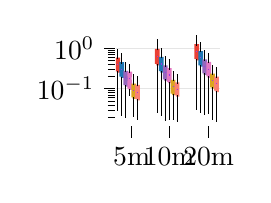
\begin{tikzpicture}

\definecolor{color0}{rgb}{0.91796875,0.25,0.203125}
\definecolor{color1}{rgb}{0.6328125,0.203125,0.91796875}
\definecolor{color2}{rgb}{0.12156862745098,0.466666666666667,0.705882352941177}
\definecolor{color3}{rgb}{0.580392156862745,0.403921568627451,0.741176470588235}
\definecolor{color4}{rgb}{0.890196078431372,0.466666666666667,0.76078431372549}
\definecolor{color5}{rgb}{0.854901960784314,0.647058823529412,0.125490196078431}
\definecolor{color6}{rgb}{0.980392156862745,0.501960784313725,0.447058823529412}
\definecolor{color7}{rgb}{0.627450980392157,0.32156862745098,0.176470588235294}
\begin{axis}[
    height=\figureheight,
    width=\figurewidth,
    axis line style={white},
    tick align=outside,
    tick pos=left,
    x grid style={white!69.0196078431373!black},
    xtick style={color=black},
    y grid style={white!90!black},
    ymajorgrids,
    ytick style={color=black},
    scaled y ticks = false,
    legend cell align={left},
    legend style={
      fill opacity=0.8,
      draw opacity=0.666,
      text opacity=1,
      at={(0.97,0.97)},
      anchor=north east,
      draw=white!80!black
    },
    tick align=outside,
    tick pos=left,
    %
    %
    %
    %
    %
    log basis y={10},
    % tick align=outside,
    % tick pos=left,
    % title={XY Positioning Errors Based on Different Anchor Distribution at Heights of 5, 10 and 20 meters},
    % x grid style={white!69.0196078431373!black},
    xmin=-0.5, xmax=26,
    % xtick style={color=black},
    xtick={3.5,13,23},
    xticklabels={5m,10m,20m},
    % y grid style={white!69.0196078431373!black},
    ymin=0.0121792364992461, ymax=2.7,
    ymode=log,
    % ytick style={color=black}
]
\addplot [line width=1pt, color0, forget plot]
table {%
-0.25 0.267748689224108
0.25 0.267748689224108
0.25 0.380422291537089
0.125 0.402042198596066
0.25 0.423662105655043
0.25 0.540741019327665
-0.25 0.540741019327665
-0.25 0.423662105655043
-0.125 0.402042198596066
-0.25 0.380422291537089
-0.25 0.267748689224108
};
\addplot [black, forget plot]
table {%
0 0.267748689224108
0 0.0289863848772585
};
\addplot [black, forget plot]
table {%
0 0.540741019327665
0 0.938178985882469
};
\addplot [black, forget plot]
table {%
-0.125 0.0289863848772585
0.125 0.0289863848772585
};
\addplot [black, forget plot]
table {%
-0.125 0.938178985882469
0.125 0.938178985882469
};
\addplot [line width=1pt, color2, forget plot]
table {%
0.75 0.199146832577806
1.25 0.199146832577806
1.25 0.285572178249853
1.125 0.296354302187928
1.25 0.307136426126003
1.25 0.41718620999352
0.75 0.41718620999352
0.75 0.307136426126003
0.875 0.296354302187928
0.75 0.285572178249853
0.75 0.199146832577806
};
\addplot [black, forget plot]
table {%
1 0.199146832577806
1 0.0221554829621503
};
\addplot [black, forget plot]
table {%
1 0.41718620999352
1 0.725403224694962
};
\addplot [black, forget plot]
table {%
0.875 0.0221554829621503
1.125 0.0221554829621503
};
\addplot [black, forget plot]
table {%
0.875 0.725403224694962
1.125 0.725403224694962
};
\addplot [line width=1pt, color3, forget plot]
table {%
1.75 0.122469708821314
2.25 0.122469708821314
2.25 0.181641926336092
2.125 0.1869526851578
2.25 0.192263443979508
2.25 0.252602811489425
1.75 0.252602811489425
1.75 0.192263443979508
1.875 0.1869526851578
1.75 0.181641926336092
1.75 0.122469708821314
};
\addplot [black, forget plot]
table {%
2 0.122469708821314
2 0.0190030769275357
};
\addplot [black, forget plot]
table {%
2 0.252602811489425
2 0.44577408615749
};
\addplot [black, forget plot]
table {%
1.875 0.0190030769275357
2.125 0.0190030769275357
};
\addplot [black, forget plot]
table {%
1.875 0.44577408615749
2.125 0.44577408615749
};
\addplot [line width=1pt, color4, forget plot]
table {%
2.75 0.100650902766832
3.25 0.100650902766832
3.25 0.137695124867848
3.125 0.180440185442575
3.25 0.223185246017302
3.25 0.242122144845884
2.75 0.242122144845884
2.75 0.223185246017302
2.875 0.180440185442575
2.75 0.137695124867848
2.75 0.100650902766832
};
\addplot [black, forget plot]
table {%
3 0.100650902766832
3 0.0682350208985586
};
\addplot [black, forget plot]
table {%
3 0.242122144845884
3 0.389030569181723
};
\addplot [black, forget plot]
table {%
2.875 0.0682350208985586
3.125 0.0682350208985586
};
\addplot [black, forget plot]
table {%
2.875 0.389030569181723
3.125 0.389030569181723
};
\addplot [line width=1pt, color5, forget plot]
table {%
3.75 0.0607649047988895
4.25 0.0607649047988895
4.25 0.0862576576249138
4.125 0.0920372953709989
4.25 0.097816933117084
4.25 0.12367095135829
3.75 0.12367095135829
3.75 0.097816933117084
3.875 0.0920372953709989
3.75 0.0862576576249138
3.75 0.0607649047988895
};
\addplot [black, forget plot]
table {%
4 0.0607649047988895
4 0.020822119488361
};
\addplot [black, forget plot]
table {%
4 0.12367095135829
4 0.217756250499344
};
\addplot [black, forget plot]
table {%
3.875 0.020822119488361
4.125 0.020822119488361
};
\addplot [black, forget plot]
table {%
3.875 0.217756250499344
4.125 0.217756250499344
};
\addplot [line width=1pt, color6, forget plot]
table {%
4.75 0.0556913103226022
5.25 0.0556913103226022
5.25 0.0786771373423886
5.125 0.0817044050322383
5.25 0.084731672722088
5.25 0.114271668637913
4.75 0.114271668637913
4.75 0.084731672722088
4.875 0.0817044050322383
4.75 0.0786771373423886
4.75 0.0556913103226022
};
\addplot [black, forget plot]
table {%
5 0.0556913103226022
5 0.0175228460953954
};
\addplot [black, forget plot]
table {%
5 0.114271668637913
5 0.196317614162956
};
\addplot [black, forget plot]
table {%
4.875 0.0175228460953954
5.125 0.0175228460953954
};
\addplot [black, forget plot]
table {%
4.875 0.196317614162956
5.125 0.196317614162956
};
\addplot [line width=1pt, color0, forget plot]
table {%
9.75 0.408592308894418
10.25 0.408592308894418
10.25 0.614751589925902
10.125 0.629718221922042
10.25 0.644684853918182
10.25 0.882559915796015
9.75 0.882559915796015
9.75 0.644684853918182
9.875 0.629718221922042
9.75 0.614751589925902
9.75 0.408592308894418
};
\addplot [black, forget plot]
table {%
10 0.408592308894418
10 0.0257120345461416
};
\addplot [black, forget plot]
table {%
10 0.882559915796015
10 1.58661217873701
};
\addplot [black, forget plot]
table {%
9.875 0.0257120345461416
10.125 0.0257120345461416
};
\addplot [black, forget plot]
table {%
9.875 1.58661217873701
10.125 1.58661217873701
};
\addplot [line width=1pt, color2, forget plot]
table {%
10.75 0.270411753121217
11.25 0.270411753121217
11.25 0.398947513784682
11.125 0.407608300536875
11.25 0.416269087289068
11.25 0.56043092783994
10.75 0.56043092783994
10.75 0.416269087289068
10.875 0.407608300536875
10.75 0.398947513784682
10.75 0.270411753121217
};
\addplot [black, forget plot]
table {%
11 0.270411753121217
11 0.0216033450685082
};
\addplot [black, forget plot]
table {%
11 0.56043092783994
11 0.995371030832681
};
\addplot [black, forget plot]
table {%
10.875 0.0216033450685082
11.125 0.0216033450685082
};
\addplot [black, forget plot]
table {%
10.875 0.995371030832681
11.125 0.995371030832681
};
\addplot [line width=1pt, color3, forget plot]
table {%
11.75 0.169999533881554
12.25 0.169999533881554
12.25 0.24935242907228
12.125 0.254374246438754
12.25 0.259396063805227
12.25 0.348406277943803
11.75 0.348406277943803
11.75 0.259396063805227
11.875 0.254374246438754
11.75 0.24935242907228
11.75 0.169999533881554
};
\addplot [black, forget plot]
table {%
12 0.169999533881554
12 0.0168244762428208
};
\addplot [black, forget plot]
table {%
12 0.348406277943803
12 0.615824007803738
};
\addplot [black, forget plot]
table {%
11.875 0.0168244762428208
12.125 0.0168244762428208
};
\addplot [black, forget plot]
table {%
11.875 0.615824007803738
12.125 0.615824007803738
};
\addplot [line width=1pt, color4, forget plot]
table {%
12.75 0.147622308785556
13.25 0.147622308785556
13.25 0.213735129413506
13.125 0.218114349898663
13.25 0.222493570383819
13.25 0.296426309281169
12.75 0.296426309281169
12.75 0.222493570383819
12.875 0.218114349898663
12.75 0.213735129413506
12.75 0.147622308785556
};
\addplot [black, forget plot]
table {%
13 0.147622308785556
13 0.0170454813000494
};
\addplot [black, forget plot]
table {%
13 0.296426309281169
13 0.519349608449588
};
\addplot [black, forget plot]
table {%
12.875 0.0170454813000494
13.125 0.0170454813000494
};
\addplot [black, forget plot]
table {%
12.875 0.519349608449588
13.125 0.519349608449588
};
\addplot [line width=1pt, color5, forget plot]
table {%
13.75 0.0754627291694511
14.25 0.0754627291694511
14.25 0.108231322644867
14.125 0.110522266179982
14.25 0.112813209715097
14.25 0.152717673112857
13.75 0.152717673112857
13.75 0.112813209715097
13.875 0.110522266179982
13.75 0.108231322644867
13.75 0.0754627291694511
};
\addplot [black, forget plot]
table {%
14 0.0754627291694511
14 0.0170589597398843
};
\addplot [black, forget plot]
table {%
14 0.152717673112857
14 0.26858580360913
};
\addplot [black, forget plot]
table {%
13.875 0.0170589597398843
14.125 0.0170589597398843
};
\addplot [black, forget plot]
table {%
13.875 0.26858580360913
14.125 0.26858580360913
};
\addplot [line width=1pt, color6, forget plot]
table {%
14.75 0.0685910707322913
15.25 0.0685910707322913
15.25 0.0951667561802471
15.125 0.0970642434279673
15.25 0.0989617306756875
15.25 0.131773894178534
14.75 0.131773894178534
14.75 0.0989617306756875
14.875 0.0970642434279673
14.75 0.0951667561802471
14.75 0.0685910707322913
};
\addplot [black, forget plot]
table {%
15 0.0685910707322913
15 0.0159748532062701
};
\addplot [black, forget plot]
table {%
15 0.131773894178534
15 0.225839574739747
};
\addplot [black, forget plot]
table {%
14.875 0.0159748532062701
15.125 0.0159748532062701
};
\addplot [black, forget plot]
table {%
14.875 0.225839574739747
15.125 0.225839574739747
};
\addplot [line width=1pt, color0]
table {%
19.75 0.543204002946311
20.25 0.543204002946311
20.25 0.798597997099198
20.125 0.818748914991217
20.25 0.838899832883236
20.25 1.15633461664651
19.75 1.15633461664651
19.75 0.838899832883236
19.875 0.818748914991217
19.75 0.798597997099198
19.75 0.543204002946311
};
%\addlegendentry{0.6 * 0.6}
\addplot [black, forget plot]
table {%
20 0.543204002946311
20 0.0313717527383977
};
\addplot [black, forget plot]
table {%
20 1.15633461664651
20 2.07390453303983
};
\addplot [black, forget plot]
table {%
19.875 0.0313717527383977
20.125 0.0313717527383977
};
\addplot [black, forget plot]
table {%
19.875 2.07390453303983
20.125 2.07390453303983
};
\addplot [line width=1pt, color2]
table {%
20.75 0.37701833424468
21.25 0.37701833424468
21.25 0.56112356640943
21.125 0.573587106041786
21.25 0.586050645674142
21.25 0.784445170834763
20.75 0.784445170834763
20.75 0.586050645674142
20.875 0.573587106041786
20.75 0.56112356640943
20.75 0.37701833424468
};
%\addlegendentry{1.2 * 1.2}
\addplot [black, forget plot]
table {%
21 0.37701833424468
21 0.02582118812503
};
\addplot [black, forget plot]
table {%
21 0.784445170834763
21 1.39212376078707
};
\addplot [black, forget plot]
table {%
20.875 0.02582118812503
21.125 0.02582118812503
};
\addplot [black, forget plot]
table {%
20.875 1.39212376078707
21.125 1.39212376078707
};
\addplot [line width=1pt, color3]
table {%
21.75 0.238474403162383
22.25 0.238474403162383
22.25 0.349930302367258
22.125 0.35733482937228
22.25 0.364739356377302
22.25 0.489280085348413
21.75 0.489280085348413
21.75 0.364739356377302
21.875 0.35733482937228
21.75 0.349930302367258
21.75 0.238474403162383
};
%\addlegendentry{3.0 * 3.0}
\addplot [black, forget plot]
table {%
22 0.238474403162383
22 0.0235558706826258
};
\addplot [black, forget plot]
table {%
22 0.489280085348413
22 0.863779716296875
};
\addplot [black, forget plot]
table {%
21.875 0.0235558706826258
22.125 0.0235558706826258
};
\addplot [black, forget plot]
table {%
21.875 0.863779716296875
22.125 0.863779716296875
};
\addplot [line width=1pt, color4]
table {%
22.75 0.20011072578637
23.25 0.20011072578637
23.25 0.295821113476713
23.125 0.302825756972492
23.25 0.309830400468271
23.25 0.423099295142593
22.75 0.423099295142593
22.75 0.309830400468271
22.875 0.302825756972492
22.75 0.295821113476713
22.75 0.20011072578637
};
%\addlegendentry{4.0 * 4.0}
\addplot [black, forget plot]
table {%
23 0.20011072578637
23 0.0243695519058795
};
\addplot [black, forget plot]
table {%
23 0.423099295142593
23 0.750056041116286
};
\addplot [black, forget plot]
table {%
22.875 0.0243695519058795
23.125 0.0243695519058795
};
\addplot [black, forget plot]
table {%
22.875 0.750056041116286
23.125 0.750056041116286
};
\addplot [line width=1pt, color5]
table {%
23.75 0.108064995157825
24.25 0.108064995157825
24.25 0.156778580518887
24.125 0.160214851769709
24.25 0.163651123020531
24.25 0.218415813802932
23.75 0.218415813802932
23.75 0.163651123020531
23.875 0.160214851769709
23.75 0.156778580518887
23.75 0.108064995157825
};
%\addlegendentry{12.0 * 12.0}
\addplot [black, forget plot]
table {%
24 0.108064995157825
24 0.0171870258574892
};
\addplot [black, forget plot]
table {%
24 0.218415813802932
24 0.382749686126767
};
\addplot [black, forget plot]
table {%
23.875 0.0171870258574892
24.125 0.0171870258574892
};
\addplot [black, forget plot]
table {%
23.875 0.382749686126767
24.125 0.382749686126767
};
\addplot [line width=1pt, color6]
table {%
24.75 0.0894885453054579
25.25 0.0894885453054579
25.25 0.131249017467418
25.125 0.134156267775655
25.25 0.137063518083893
25.25 0.184470957947186
24.75 0.184470957947186
24.75 0.137063518083893
24.875 0.134156267775655
24.75 0.131249017467418
24.75 0.0894885453054579
};
%\addlegendentry{16.0 * 16.0}
\addplot [black, forget plot]
table {%
25 0.0894885453054579
25 0.0155548630651615
};
\addplot [black, forget plot]
table {%
25 0.184470957947186
25 0.324447204356026
};
\addplot [black, forget plot]
table {%
24.875 0.0155548630651615
25.125 0.0155548630651615
};
\addplot [black, forget plot]
table {%
24.875 0.324447204356026
25.125 0.324447204356026
};
\addplot [color1, forget plot]
table {%
-0.125 0.402042198596066
0.125 0.402042198596066
};
\addplot [color1, forget plot]
table {%
0.875 0.296354302187928
1.125 0.296354302187928
};
\addplot [color1, forget plot]
table {%
1.875 0.1869526851578
2.125 0.1869526851578
};
\addplot [color1, forget plot]
table {%
2.875 0.180440185442575
3.125 0.180440185442575
};
\addplot [color1, forget plot]
table {%
3.875 0.0920372953709989
4.125 0.0920372953709989
};
\addplot [color1, forget plot]
table {%
4.875 0.0817044050322383
5.125 0.0817044050322383
};
\addplot [color1, forget plot]
table {%
9.875 0.629718221922042
10.125 0.629718221922042
};
\addplot [color1, forget plot]
table {%
10.875 0.407608300536875
11.125 0.407608300536875
};
\addplot [color1, forget plot]
table {%
11.875 0.254374246438754
12.125 0.254374246438754
};
\addplot [color1, forget plot]
table {%
12.875 0.218114349898663
13.125 0.218114349898663
};
\addplot [color1, forget plot]
table {%
13.875 0.110522266179982
14.125 0.110522266179982
};
\addplot [color1, forget plot]
table {%
14.875 0.0970642434279673
15.125 0.0970642434279673
};
\addplot [color1, forget plot]
table {%
19.875 0.818748914991217
20.125 0.818748914991217
};
\addplot [color1, forget plot]
table {%
20.875 0.573587106041786
21.125 0.573587106041786
};
\addplot [color1, forget plot]
table {%
21.875 0.35733482937228
22.125 0.35733482937228
};
\addplot [color1, forget plot]
table {%
22.875 0.302825756972492
23.125 0.302825756972492
};
\addplot [color1, forget plot]
table {%
23.875 0.160214851769709
24.125 0.160214851769709
};
\addplot [color1, forget plot]
table {%
24.875 0.134156267775655
25.125 0.134156267775655
};
\end{axis}

\end{tikzpicture}
}
        \caption{Positioning $xy$ error.}
        \label{fig:square_pos_xy}
    \end{subfigure}
    \begin{subfigure}{0.32\textwidth}
        \centering
        \setlength\figureheight{\textwidth}
        \setlength\figurewidth{\textwidth}
        \footnotesize{% This file was created by tikzplotlib v0.9.8.
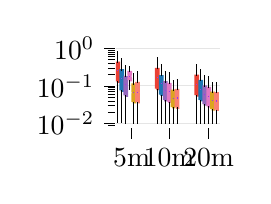
\begin{tikzpicture}

% \definecolor{color0}{rgb}{0.91796875,0.25,0.203125}
% \definecolor{color1}{rgb}{1,0.498039215686275,0.0549019607843137}
% \definecolor{color2}{rgb}{0.6328125,0.203125,0.91796875}
% \definecolor{color3}{rgb}{0.171875,0.49609375,0.71875}
% \definecolor{color4}{rgb}{0.49609375,0.80078125,0.73046875}
% \definecolor{color5}{rgb}{0.92578125,0.96875,0.69140625}
% \definecolor{color6}{rgb}{0.16796875,0.546875,0.7421875}

\definecolor{color0}{rgb}{0.91796875,0.25,0.203125}
\definecolor{color1}{rgb}{0.6328125,0.203125,0.91796875}
\definecolor{color2}{rgb}{0.12156862745098,0.466666666666667,0.705882352941177}
\definecolor{color3}{rgb}{0.580392156862745,0.403921568627451,0.741176470588235}
\definecolor{color4}{rgb}{0.890196078431372,0.466666666666667,0.76078431372549}
\definecolor{color5}{rgb}{0.854901960784314,0.647058823529412,0.125490196078431}
\definecolor{color6}{rgb}{0.980392156862745,0.501960784313725,0.447058823529412}
\definecolor{color7}{rgb}{0.627450980392157,0.32156862745098,0.176470588235294}

\begin{axis}[
    height=\figureheight,
    width=\figurewidth,
    axis line style={white},
    tick align=outside,
    tick pos=left,
    x grid style={white!69.0196078431373!black},
    xtick style={color=black},
    y grid style={white!90!black},
    ymajorgrids,
    ytick style={color=black},
    scaled y ticks = false,
    legend cell align={left},
    legend style={
      fill opacity=0.8,
      draw opacity=0.666,
      text opacity=1,
      at={(0.97,0.97)},
      anchor=north east,
      draw=white!80!black
    },
    tick align=outside,
    tick pos=left,
    %
    %
    %
    %
    %
    %
    %
    log basis y={10},
    % tick align=outside,
    % tick pos=left,
    % title={Z Positioning Errors Based on Different Anchor Distribution at Heights of 5, 10 and 20 meters},
    % x grid style={white!69.0196078431373!black},
    xmin=-0.5, xmax=26,
    % xtick style={color=black},
    xtick={3.5,13,23},
    xticklabels={5m,10m,20m},
    % y grid style={white!69.0196078431373!black},
    ymin=0.00804930865024464, ymax=2.7,
    ymode=log,
    % ytick style={color=black}
]
\addplot [line width=1pt, color0, forget plot]
table {%
-0.25 0.130141935348511
0.25 0.130141935348511
0.25 0.230974399622699
0.125 0.25279392242425
0.25 0.274613445225802
0.25 0.405654792785606
-0.25 0.405654792785606
-0.25 0.274613445225802
-0.125 0.25279392242425
-0.25 0.230974399622699
-0.25 0.130141935348511
};
\addplot [black, forget plot]
table {%
0 0.130141935348511
0 0.0105277442932028
};
\addplot [black, forget plot]
table {%
0 0.405654792785606
0 0.790750169758004
};
\addplot [black, forget plot]
table {%
-0.125 0.0105277442932028
0.125 0.0105277442932028
};
\addplot [black, forget plot]
table {%
-0.125 0.790750169758004
0.125 0.790750169758004
};
\addplot [line width=1pt, color2, forget plot]
table {%
0.75 0.0755092000961715
1.25 0.0755092000961715
1.25 0.145915463928272
1.125 0.154695053100452
1.25 0.163474642272633
1.25 0.253052712678886
0.75 0.253052712678886
0.75 0.163474642272633
0.875 0.154695053100452
0.75 0.145915463928272
0.75 0.0755092000961715
};
\addplot [black, forget plot]
table {%
1 0.0755092000961715
1 0.0107640838622496
};
\addplot [black, forget plot]
table {%
1 0.253052712678886
1 0.518915538787724
};
\addplot [black, forget plot]
table {%
0.875 0.0107640838622496
1.125 0.0107640838622496
};
\addplot [black, forget plot]
table {%
0.875 0.518915538787724
1.125 0.518915538787724
};
\addplot [line width=1pt, color3, forget plot]
table {%
1.75 0.0555655145647236
2.25 0.0555655145647236
2.25 0.103259641365462
2.125 0.107861089706383
2.25 0.112462538047304
2.25 0.168317904472438
1.75 0.168317904472438
1.75 0.112462538047304
1.875 0.107861089706383
1.75 0.103259641365462
1.75 0.0555655145647236
};
\addplot [black, forget plot]
table {%
2 0.0555655145647236
2 0.0100500679016999
};
\addplot [black, forget plot]
table {%
2 0.168317904472438
2 0.33585695266694
};
\addplot [black, forget plot]
table {%
1.875 0.0100500679016999
2.125 0.0100500679016999
};
\addplot [black, forget plot]
table {%
1.875 0.33585695266694
2.125 0.33585695266694
};
\addplot [line width=1pt, color4, forget plot]
table {%
2.75 0.14326691865921
3.25 0.14326691865921
3.25 0.155488057995789
3.125 0.181300792694087
3.25 0.207113527392385
3.25 0.228698067665099
2.75 0.228698067665099
2.75 0.207113527392385
2.875 0.181300792694087
2.75 0.155488057995789
2.75 0.14326691865921
};
\addplot [black, forget plot]
table {%
3 0.14326691865921
3 0.0823523235321049
};
\addplot [black, forget plot]
table {%
3 0.228698067665099
3 0.315878238677976
};
\addplot [black, forget plot]
table {%
2.875 0.0823523235321049
3.125 0.0823523235321049
};
\addplot [black, forget plot]
table {%
2.875 0.315878238677976
3.125 0.315878238677976
};
\addplot [line width=1pt, color5, forget plot]
table {%
3.75 0.037188584806001
4.25 0.037188584806001
4.25 0.0595463339217097
4.125 0.0659799957245917
4.25 0.0724136575274737
4.25 0.107213082309096
3.75 0.107213082309096
3.75 0.0724136575274737
3.875 0.0659799957245917
3.75 0.0595463339217097
3.75 0.037188584806001
};
\addplot [black, forget plot]
table {%
4 0.037188584806001
4 0.0100437736570211
};
\addplot [black, forget plot]
table {%
4 0.107213082309096
4 0.206688671112088
};
\addplot [black, forget plot]
table {%
3.875 0.0100437736570211
4.125 0.0100437736570211
};
\addplot [black, forget plot]
table {%
3.875 0.206688671112088
4.125 0.206688671112088
};
\addplot [line width=1pt, color6, forget plot]
table {%
4.75 0.0374092960358725
5.25 0.0374092960358725
5.25 0.0637865114864845
5.125 0.0678792953492469
5.25 0.0719720792120093
5.25 0.116608352660974
4.75 0.116608352660974
4.75 0.0719720792120093
4.875 0.0678792953492469
4.75 0.0637865114864845
4.75 0.0374092960358725
};
\addplot [black, forget plot]
table {%
5 0.0374092960358725
5 0.0101840400694595
};
\addplot [black, forget plot]
table {%
5 0.116608352660974
5 0.234932403564249
};
\addplot [black, forget plot]
table {%
4.875 0.0101840400694595
5.125 0.0101840400694595
};
\addplot [black, forget plot]
table {%
4.875 0.234932403564249
5.125 0.234932403564249
};
\addplot [line width=1pt, color0, forget plot]
table {%
9.75 0.0837351608281693
10.25 0.0837351608281693
10.25 0.158467680258277
10.125 0.164497737885056
10.25 0.170527795511836
10.25 0.274696760176671
9.75 0.274696760176671
9.75 0.170527795511836
9.875 0.164497737885056
9.75 0.158467680258277
9.75 0.0837351608281693
};
\addplot [black, forget plot]
table {%
10 0.0837351608281693
10 0.0101135253901852
};
\addplot [black, forget plot]
table {%
10 0.274696760176671
10 0.559741516113794
};
\addplot [black, forget plot]
table {%
9.875 0.0101135253901852
10.125 0.0101135253901852
};
\addplot [black, forget plot]
table {%
9.875 0.559741516113794
10.125 0.559741516113794
};
\addplot [line width=1pt, color2, forget plot]
table {%
10.75 0.0584935092910559
11.25 0.0584935092910559
11.25 0.108548561495518
11.125 0.112114410400578
11.25 0.115680259305637
11.25 0.17790120124874
10.75 0.17790120124874
10.75 0.115680259305637
10.875 0.112114410400578
10.75 0.108548561495518
10.75 0.0584935092910559
};
\addplot [black, forget plot]
table {%
11 0.0584935092910559
11 0.0100371932982704
};
\addplot [black, forget plot]
table {%
11 0.17790120124874
11 0.356388053895861
};
\addplot [black, forget plot]
table {%
10.875 0.0100371932982704
11.125 0.0100371932982704
};
\addplot [black, forget plot]
table {%
10.875 0.356388053895861
11.125 0.356388053895861
};
\addplot [line width=1pt, color3, forget plot]
table {%
11.75 0.0419515800471855
12.25 0.0419515800471855
12.25 0.0747838255194755
12.125 0.0770266723650668
12.25 0.0792695192106581
12.25 0.121631698608168
11.75 0.121631698608168
11.75 0.0792695192106581
11.875 0.0770266723650668
11.75 0.0747838255194755
11.75 0.0419515800471855
};
\addplot [black, forget plot]
table {%
12 0.0419515800471855
12 0.0100144958485746
};
\addplot [black, forget plot]
table {%
12 0.121631698608168
12 0.240501861572401
};
\addplot [black, forget plot]
table {%
11.875 0.0100144958485746
12.125 0.0100144958485746
};
\addplot [black, forget plot]
table {%
11.875 0.240501861572401
12.125 0.240501861572401
};
\addplot [line width=1pt, color4, forget plot]
table {%
12.75 0.0380288314826975
13.25 0.0380288314826975
13.25 0.0672714378106817
13.125 0.0693967628479921
13.25 0.0715220878853025
13.25 0.110246448516881
12.75 0.110246448516881
12.75 0.0715220878853025
12.875 0.0693967628479921
12.75 0.0672714378106817
12.75 0.0380288314826975
};
\addplot [black, forget plot]
table {%
13 0.0380288314826975
13 0.0100238418593257
};
\addplot [black, forget plot]
table {%
13 0.110246448516881
13 0.218511466981189
};
\addplot [black, forget plot]
table {%
12.875 0.0100238418593257
13.125 0.0100238418593257
};
\addplot [black, forget plot]
table {%
12.875 0.218511466981189
13.125 0.218511466981189
};
\addplot [line width=1pt, color5, forget plot]
table {%
13.75 0.0271833419782341
14.25 0.0271833419782341
14.25 0.0444245250780375
14.125 0.0457671356216505
14.25 0.0471097461652634
14.25 0.0724587059035358
13.75 0.0724587059035358
13.75 0.0471097461652634
13.875 0.0457671356216505
13.75 0.0444245250780375
13.75 0.0271833419782341
};
\addplot [black, forget plot]
table {%
14 0.0271833419782341
14 0.0101230239877399
};
\addplot [black, forget plot]
table {%
14 0.0724587059035358
14 0.138281707764149
};
\addplot [black, forget plot]
table {%
13.875 0.0101230239877399
14.125 0.0101230239877399
};
\addplot [black, forget plot]
table {%
13.875 0.138281707764149
14.125 0.138281707764149
};
\addplot [line width=1pt, color6, forget plot]
table {%
14.75 0.026636428834621
15.25 0.026636428834621
15.25 0.0458447301899036
15.125 0.0473315811158965
15.25 0.0488184320418895
15.25 0.0761458206161834
14.75 0.0761458206161834
14.75 0.0488184320418895
14.875 0.0473315811158965
14.75 0.0458447301899036
14.75 0.026636428834621
};
\addplot [black, forget plot]
table {%
15 0.026636428834621
15 0.0100228118881169
};
\addplot [black, forget plot]
table {%
15 0.0761458206161834
15 0.149344215394184
};
\addplot [black, forget plot]
table {%
14.875 0.0100228118881169
15.125 0.0100228118881169
};
\addplot [black, forget plot]
table {%
14.875 0.149344215394184
15.125 0.149344215394184
};
\addplot [line width=1pt, color0]
table {%
19.75 0.0565042877179174
20.25 0.0565042877179174
20.25 0.106138682651996
20.125 0.110221366882444
20.25 0.114304051112891
20.25 0.180727844241352
19.75 0.180727844241352
19.75 0.114304051112891
19.875 0.110221366882444
19.75 0.106138682651996
19.75 0.0565042877179174
};
%\addlegendentry{0.6 * 0.6}
\addplot [black, forget plot]
table {%
20 0.0565042877179174
20 0.0101180267357286
};
\addplot [black, forget plot]
table {%
20 0.180727844241352
20 0.364172363279252
};
\addplot [black, forget plot]
table {%
19.875 0.0101180267357286
20.125 0.0101180267357286
};
\addplot [black, forget plot]
table {%
19.875 0.364172363279252
20.125 0.364172363279252
};
\addplot [line width=1pt, color2]
table {%
20.75 0.0419956016520837
21.25 0.0419956016520837
21.25 0.0752755386822257
21.125 0.0780046844474143
21.25 0.0807338302126028
21.25 0.131210002897886
20.75 0.131210002897886
20.75 0.0807338302126028
20.875 0.0780046844474143
20.75 0.0752755386822257
20.75 0.0419956016520837
};
%\addlegendentry{1.2 * 1.2}
\addplot [black, forget plot]
table {%
21 0.0419956016520837
21 0.0100163269010558
};
\addplot [black, forget plot]
table {%
21 0.131210002897886
21 0.264321746822414
};
\addplot [black, forget plot]
table {%
20.875 0.0100163269010558
21.125 0.0100163269010558
};
\addplot [black, forget plot]
table {%
20.875 0.264321746822414
21.125 0.264321746822414
};
\addplot [line width=1pt, color3]
table {%
21.75 0.0323681831387876
22.25 0.0323681831387876
22.25 0.056350262624775
22.125 0.0581927871693484
22.25 0.0600353117139218
22.25 0.0947780609112368
21.75 0.0947780609112368
21.75 0.0600353117139218
21.875 0.0581927871693484
21.75 0.056350262624775
21.75 0.0323681831387876
};
%\addlegendentry{3.0 * 3.0}
\addplot [black, forget plot]
table {%
22 0.0323681831387876
22 0.0100195312530822
};
\addplot [black, forget plot]
table {%
22 0.0947780609112368
22 0.188052253717919
};
\addplot [black, forget plot]
table {%
21.875 0.0100195312530822
22.125 0.0100195312530822
};
\addplot [black, forget plot]
table {%
21.875 0.188052253717919
22.125 0.188052253717919
};
\addplot [line width=1pt, color4]
table {%
22.75 0.028549823758218
23.25 0.028549823758218
23.25 0.0502052770272442
23.125 0.0520056915283362
23.25 0.0538061060294283
23.25 0.085864925388818
22.75 0.085864925388818
22.75 0.0538061060294283
22.875 0.0520056915283362
22.75 0.0502052770272442
22.75 0.028549823758218
};
%\addlegendentry{4.0 * 4.0}
\addplot [black, forget plot]
table {%
23 0.028549823758218
23 0.0100192260703054
};
\addplot [black, forget plot]
table {%
23 0.085864925388818
23 0.171740417475913
};
\addplot [black, forget plot]
table {%
22.875 0.0100192260703054
23.125 0.0100192260703054
};
\addplot [black, forget plot]
table {%
22.875 0.171740417475913
23.125 0.171740417475913
};
\addplot [line width=1pt, color5]
table {%
23.75 0.0238789939916328
24.25 0.0238789939916328
24.25 0.0399971693268882
24.125 0.0412576293913816
24.25 0.0425180894558749
24.25 0.0643568229619271
23.75 0.0643568229619271
23.75 0.0425180894558749
23.875 0.0412576293913816
23.75 0.0399971693268882
23.75 0.0238789939916328
};
%\addlegendentry{12.0 * 12.0}
\addplot [black, forget plot]
table {%
24 0.0238789939916328
24 0.0100177001912805
};
\addplot [black, forget plot]
table {%
24 0.0643568229619271
24 0.124875106814798
};
\addplot [black, forget plot]
table {%
23.875 0.0100177001912805
24.125 0.0100177001912805
};
\addplot [black, forget plot]
table {%
23.875 0.124875106814798
24.125 0.124875106814798
};
\addplot [line width=1pt, color6]
table {%
24.75 0.0234525680583104
25.25 0.0234525680583104
25.25 0.0382427506698399
25.125 0.0394415283224525
25.25 0.0406403059750651
25.25 0.0626176834057919
24.75 0.0626176834057919
24.75 0.0406403059750651
24.875 0.0394415283224525
24.75 0.0382427506698399
24.75 0.0234525680583104
};
%\addlegendentry{16.0 * 16.0}
\addplot [black, forget plot]
table {%
25 0.0234525680583104
25 0.0100222015336513
};
\addplot [black, forget plot]
table {%
25 0.0626176834057919
25 0.121285095218553
};
\addplot [black, forget plot]
table {%
24.875 0.0100222015336513
25.125 0.0100222015336513
};
\addplot [black, forget plot]
table {%
24.875 0.121285095218553
25.125 0.121285095218553
};
\addplot [color1, forget plot]
table {%
-0.125 0.25279392242425
0.125 0.25279392242425
};
\addplot [color1, forget plot]
table {%
0.875 0.154695053100452
1.125 0.154695053100452
};
\addplot [color1, forget plot]
table {%
1.875 0.107861089706383
2.125 0.107861089706383
};
\addplot [color1, forget plot]
table {%
2.875 0.181300792694087
3.125 0.181300792694087
};
\addplot [color1, forget plot]
table {%
3.875 0.0659799957245917
4.125 0.0659799957245917
};
\addplot [color1, forget plot]
table {%
4.875 0.0678792953492469
5.125 0.0678792953492469
};
\addplot [color1, forget plot]
table {%
9.875 0.164497737885056
10.125 0.164497737885056
};
\addplot [color1, forget plot]
table {%
10.875 0.112114410400578
11.125 0.112114410400578
};
\addplot [color1, forget plot]
table {%
11.875 0.0770266723650668
12.125 0.0770266723650668
};
\addplot [color1, forget plot]
table {%
12.875 0.0693967628479921
13.125 0.0693967628479921
};
\addplot [color1, forget plot]
table {%
13.875 0.0457671356216505
14.125 0.0457671356216505
};
\addplot [color1, forget plot]
table {%
14.875 0.0473315811158965
15.125 0.0473315811158965
};
\addplot [color1, forget plot]
table {%
19.875 0.110221366882444
20.125 0.110221366882444
};
\addplot [color1, forget plot]
table {%
20.875 0.0780046844474143
21.125 0.0780046844474143
};
\addplot [color1, forget plot]
table {%
21.875 0.0581927871693484
22.125 0.0581927871693484
};
\addplot [color1, forget plot]
table {%
22.875 0.0520056915283362
23.125 0.0520056915283362
};
\addplot [color1, forget plot]
table {%
23.875 0.0412576293913816
24.125 0.0412576293913816
};
\addplot [color1, forget plot]
table {%
24.875 0.0394415283224525
25.125 0.0394415283224525
};
\end{axis}

\end{tikzpicture}
}
        \caption{Positioning $z$ error.}
        \label{fig:square_pos_z}
    \end{subfigure}
        \begin{subfigure}{0.32\textwidth}
        \centering
        \setlength\figureheight{\textwidth}
        \setlength\figurewidth{\textwidth}
        \footnotesize{% This file was created by tikzplotlib v0.9.8.
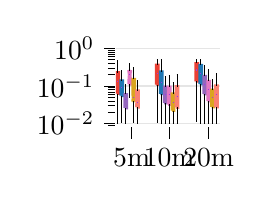
\begin{tikzpicture}

\definecolor{color0}{rgb}{0.91796875,0.25,0.203125}
\definecolor{color1}{rgb}{0.6328125,0.203125,0.91796875}
\definecolor{color2}{rgb}{0.12156862745098,0.466666666666667,0.705882352941177}
\definecolor{color3}{rgb}{0.580392156862745,0.403921568627451,0.741176470588235}
\definecolor{color4}{rgb}{0.890196078431372,0.466666666666667,0.76078431372549}
\definecolor{color5}{rgb}{0.854901960784314,0.647058823529412,0.125490196078431}
\definecolor{color6}{rgb}{0.980392156862745,0.501960784313725,0.447058823529412}
\definecolor{color7}{rgb}{0.627450980392157,0.32156862745098,0.176470588235294}

\begin{axis}[
    height=\figureheight,
    width=\figurewidth,
    axis line style={white},
    tick align=outside,
    tick pos=left,
    x grid style={white!69.0196078431373!black},
    xtick style={color=black},
    y grid style={white!90!black},
    ymajorgrids,
    ytick style={color=black},
    scaled y ticks = false,
    legend cell align={left},
    legend style={
      fill opacity=0.8,
      draw opacity=0.666,
      text opacity=1,
      at={(0.97,0.97)},
      anchor=north east,
      draw=white!80!black
    },
    tick align=outside,
    tick pos=left,
    %
    %
    %
    %
    %
    %
    %
    log basis y={10},
    % tick align=outside,
    % tick pos=left,
    % title={XY Navigation Errors Based on Different Anchor Distribution at Heights of 5, 10 and 20 meters},
    % x grid style={white!69.0196078431373!black},
    xmin=-0.5, xmax=26,
    % xtick style={color=black},
    xtick={3.5,13,23},
    xticklabels={5m,10m,20m},
    % y grid style={white!69.0196078431373!black},
    ymin=0.00823407310056917, ymax=2.7,
    ymode=log,
    % ytick style={color=black}
]
\addplot [line width=1pt, color0, forget plot]
table {%
-0.25 0.0629254579544067
0.25 0.0629254579544067
0.25 0.116854261331483
0.125 0.133378744125366
0.25 0.149903226919249
0.25 0.225299537181854
-0.25 0.225299537181854
-0.25 0.149903226919249
-0.125 0.133378744125366
-0.25 0.116854261331483
-0.25 0.0629254579544067
};
\addplot [black, forget plot]
table {%
0 0.0629254579544067
0 0.0100212097167969
};
\addplot [black, forget plot]
table {%
0 0.225299537181854
0 0.464566707611084
};
\addplot [black, forget plot]
table {%
-0.125 0.0100212097167969
0.125 0.0100212097167969
};
\addplot [black, forget plot]
table {%
-0.125 0.464566707611084
0.125 0.464566707611084
};
\addplot [line width=1pt, color2, forget plot]
table {%
0.75 0.0550479888916016
1.25 0.0550479888916016
1.25 0.0872549469128582
1.125 0.0913627147674561
1.25 0.0954704826220539
1.25 0.136493682861328
0.75 0.136493682861328
0.75 0.0954704826220539
0.875 0.0913627147674561
0.75 0.0872549469128582
0.75 0.0550479888916016
};
\addplot [black, forget plot]
table {%
1 0.0550479888916016
1 0.0105924606323242
};
\addplot [black, forget plot]
table {%
1 0.136493682861328
1 0.256451845169067
};
\addplot [black, forget plot]
table {%
0.875 0.0105924606323242
1.125 0.0105924606323242
};
\addplot [black, forget plot]
table {%
0.875 0.256451845169067
1.125 0.256451845169067
};
\addplot [line width=1pt, color3, forget plot]
table {%
1.75 0.0262908935546875
2.25 0.0262908935546875
2.25 0.0422004902930734
2.125 0.0437288284301758
2.25 0.0452571665672782
2.25 0.0594601631164551
1.75 0.0594601631164551
1.75 0.0452571665672782
1.875 0.0437288284301758
1.75 0.0422004902930734
1.75 0.0262908935546875
};
\addplot [black, forget plot]
table {%
2 0.0262908935546875
2 0.010059118270874
};
\addplot [black, forget plot]
table {%
2 0.0594601631164551
2 0.108749151229858
};
\addplot [black, forget plot]
table {%
1.875 0.010059118270874
2.125 0.010059118270874
};
\addplot [black, forget plot]
table {%
1.875 0.108749151229858
2.125 0.108749151229858
};
\addplot [line width=1pt, color4, forget plot]
table {%
2.75 0.111529111862183
3.25 0.111529111862183
3.25 0.130515317329696
3.125 0.196047306060791
3.25 0.261579294791886
3.25 0.24996542930603
2.75 0.24996542930603
2.75 0.261579294791886
2.875 0.196047306060791
2.75 0.130515317329696
2.75 0.111529111862183
};
\addplot [black, forget plot]
table {%
3 0.111529111862183
3 0.0505809783935547
};
\addplot [black, forget plot]
table {%
3 0.24996542930603
3 0.389389276504517
};
\addplot [black, forget plot]
table {%
2.875 0.0505809783935547
3.125 0.0505809783935547
};
\addplot [black, forget plot]
table {%
2.875 0.389389276504517
3.125 0.389389276504517
};
\addplot [line width=1pt, color5, forget plot]
table {%
3.75 0.0398937463760376
4.25 0.0398937463760376
4.25 0.0386781307707235
4.125 0.0503287315368652
4.25 0.061979332303007
4.25 0.150957584381104
3.75 0.150957584381104
3.75 0.061979332303007
3.875 0.0503287315368652
3.75 0.0386781307707235
3.75 0.0398937463760376
};
\addplot [black, forget plot]
table {%
4 0.0398937463760376
4 0.0105338096618652
};
\addplot [black, forget plot]
table {%
4 0.150957584381104
4 0.312473297119141
};
\addplot [black, forget plot]
table {%
3.875 0.0105338096618652
4.125 0.0105338096618652
};
\addplot [black, forget plot]
table {%
3.875 0.312473297119141
4.125 0.312473297119141
};
\addplot [line width=1pt, color6, forget plot]
table {%
4.75 0.0273342132568359
5.25 0.0273342132568359
5.25 0.0339629243246975
5.125 0.0363602638244629
5.25 0.0387576033242283
5.25 0.0742993354797363
4.75 0.0742993354797363
4.75 0.0387576033242283
4.875 0.0363602638244629
4.75 0.0339629243246975
4.75 0.0273342132568359
};
\addplot [black, forget plot]
table {%
5 0.0273342132568359
5 0.010307788848877
};
\addplot [black, forget plot]
table {%
5 0.0742993354797363
5 0.141448497772217
};
\addplot [black, forget plot]
table {%
4.875 0.010307788848877
5.125 0.010307788848877
};
\addplot [black, forget plot]
table {%
4.875 0.141448497772217
5.125 0.141448497772217
};
\addplot [line width=1pt, color0, forget plot]
table {%
9.75 0.109080791473389
10.25 0.109080791473389
10.25 0.208775860281895
10.125 0.217644453048706
10.25 0.226513045815517
10.25 0.355952739715576
9.75 0.355952739715576
9.75 0.226513045815517
9.875 0.217644453048706
9.75 0.208775860281895
9.75 0.109080791473389
};
\addplot [black, forget plot]
table {%
10 0.109080791473389
10 0.0106794834136963
};
\addplot [black, forget plot]
table {%
10 0.355952739715576
10 0.499023914337158
};
\addplot [black, forget plot]
table {%
9.875 0.0106794834136963
10.125 0.0106794834136963
};
\addplot [black, forget plot]
table {%
9.875 0.499023914337158
10.125 0.499023914337158
};
\addplot [line width=1pt, color2, forget plot]
table {%
10.75 0.061793327331543
11.25 0.061793327331543
11.25 0.119313400273
11.125 0.124480247497559
11.25 0.129647094722117
11.25 0.237082719802856
10.75 0.237082719802856
10.75 0.129647094722117
10.875 0.124480247497559
10.75 0.119313400273
10.75 0.061793327331543
};
\addplot [black, forget plot]
table {%
11 0.061793327331543
11 0.0100317001342773
};
\addplot [black, forget plot]
table {%
11 0.237082719802856
11 0.498574733734131
};
\addplot [black, forget plot]
table {%
10.875 0.0100317001342773
11.125 0.0100317001342773
};
\addplot [black, forget plot]
table {%
10.875 0.498574733734131
11.125 0.498574733734131
};
\addplot [line width=1pt, color3, forget plot]
table {%
11.75 0.0356164574623108
12.25 0.0356164574623108
12.25 0.0590718957655501
12.125 0.0608000755310059
12.25 0.0625282552964616
12.25 0.0943392515182495
11.75 0.0943392515182495
11.75 0.0625282552964616
11.875 0.0608000755310059
11.75 0.0590718957655501
11.75 0.0356164574623108
};
\addplot [black, forget plot]
table {%
12 0.0356164574623108
12 0.0100545883178711
};
\addplot [black, forget plot]
table {%
12 0.0943392515182495
12 0.180632591247559
};
\addplot [black, forget plot]
table {%
11.875 0.0100545883178711
12.125 0.0100545883178711
};
\addplot [black, forget plot]
table {%
11.875 0.180632591247559
12.125 0.180632591247559
};
\addplot [line width=1pt, color4, forget plot]
table {%
12.75 0.0324709415435791
13.25 0.0324709415435791
13.25 0.0561843826720145
13.125 0.0580892562866211
13.25 0.0599941299012277
13.25 0.0934865474700928
12.75 0.0934865474700928
12.75 0.0599941299012277
12.875 0.0580892562866211
12.75 0.0561843826720145
12.75 0.0324709415435791
};
\addplot [black, forget plot]
table {%
13 0.0324709415435791
13 0.0100338459014893
};
\addplot [black, forget plot]
table {%
13 0.0934865474700928
13 0.184965848922729
};
\addplot [black, forget plot]
table {%
12.875 0.0100338459014893
13.125 0.0100338459014893
};
\addplot [black, forget plot]
table {%
12.875 0.184965848922729
13.125 0.184965848922729
};
\addplot [line width=1pt, color5, forget plot]
table {%
13.75 0.0223686695098877
14.25 0.0223686695098877
14.25 0.035463001367267
14.125 0.0366926193237305
14.25 0.0379222372801939
14.25 0.062411367893219
13.75 0.062411367893219
13.75 0.0379222372801939
13.875 0.0366926193237305
13.75 0.035463001367267
13.75 0.0223686695098877
};
\addplot [black, forget plot]
table {%
14 0.0223686695098877
14 0.0100116729736328
};
\addplot [black, forget plot]
table {%
14 0.062411367893219
14 0.121386528015137
};
\addplot [black, forget plot]
table {%
13.875 0.0100116729736328
14.125 0.0100116729736328
};
\addplot [black, forget plot]
table {%
13.875 0.121386528015137
14.125 0.121386528015137
};
\addplot [line width=1pt, color6, forget plot]
table {%
14.75 0.0270559787750244
15.25 0.0270559787750244
15.25 0.0513307469276914
15.125 0.053499698638916
15.25 0.0556686503501407
15.25 0.0965852737426758
14.75 0.0965852737426758
14.75 0.0556686503501407
14.875 0.053499698638916
14.75 0.0513307469276914
14.75 0.0270559787750244
};
\addplot [black, forget plot]
table {%
15 0.0270559787750244
15 0.0100679397583008
};
\addplot [black, forget plot]
table {%
15 0.0965852737426758
15 0.198929309844971
};
\addplot [black, forget plot]
table {%
14.875 0.0100679397583008
15.125 0.0100679397583008
};
\addplot [black, forget plot]
table {%
14.875 0.198929309844971
15.125 0.198929309844971
};
\addplot [line width=1pt, color0]
table {%
19.75 0.133109569549561
20.25 0.133109569549561
20.25 0.251491091482432
20.125 0.263442993164062
20.25 0.275394894845693
20.25 0.394724369049072
19.75 0.394724369049072
19.75 0.275394894845693
19.875 0.263442993164062
19.75 0.251491091482432
19.75 0.133109569549561
};
%\addlegendentry{0.6 * 0.6}
\addplot [black, forget plot]
table {%
20 0.133109569549561
20 0.0112812519073486
};
\addplot [black, forget plot]
table {%
20 0.394724369049072
20 0.498894691467285
};
\addplot [black, forget plot]
table {%
19.875 0.0112812519073486
20.125 0.0112812519073486
};
\addplot [black, forget plot]
table {%
19.875 0.498894691467285
20.125 0.498894691467285
};
\addplot [line width=1pt, color2]
table {%
20.75 0.112098932266235
21.25 0.112098932266235
21.25 0.204240932496009
21.125 0.21213698387146
21.25 0.220033035246911
21.25 0.353559255599976
20.75 0.353559255599976
20.75 0.220033035246911
20.875 0.21213698387146
20.75 0.204240932496009
20.75 0.112098932266235
};
%\addlegendentry{1.2 * 1.2}
\addplot [black, forget plot]
table {%
21 0.112098932266235
21 0.010089635848999
};
\addplot [black, forget plot]
table {%
21 0.353559255599976
21 0.499281406402588
};
\addplot [black, forget plot]
table {%
20.875 0.010089635848999
21.125 0.010089635848999
};
\addplot [black, forget plot]
table {%
20.875 0.499281406402588
21.125 0.499281406402588
};
\addplot [line width=1pt, color3]
table {%
21.75 0.0613045692443848
22.25 0.0613045692443848
22.25 0.107318790443975
22.125 0.11083984375
22.25 0.114360897056025
22.25 0.179744243621826
21.75 0.179744243621826
21.75 0.114360897056025
21.875 0.11083984375
21.75 0.107318790443975
21.75 0.0613045692443848
};
%\addlegendentry{3.0 * 3.0}
\addplot [black, forget plot]
table {%
22 0.0613045692443848
22 0.0102958679199219
};
\addplot [black, forget plot]
table {%
22 0.179744243621826
22 0.353663444519043
};
\addplot [black, forget plot]
table {%
21.875 0.0102958679199219
22.125 0.0102958679199219
};
\addplot [black, forget plot]
table {%
21.875 0.353663444519043
22.125 0.353663444519043
};
\addplot [line width=1pt, color4]
table {%
22.75 0.0401172637939453
23.25 0.0401172637939453
23.25 0.0776253280932044
23.125 0.0806457996368408
23.25 0.0836662711804773
23.25 0.13330078125
22.75 0.13330078125
22.75 0.0836662711804773
22.875 0.0806457996368408
22.75 0.0776253280932044
22.75 0.0401172637939453
};
%\addlegendentry{4.0 * 4.0}
\addplot [black, forget plot]
table {%
23 0.0401172637939453
23 0.0100553035736084
};
\addplot [black, forget plot]
table {%
23 0.13330078125
23 0.272943258285522
};
\addplot [black, forget plot]
table {%
22.875 0.0100553035736084
23.125 0.0100553035736084
};
\addplot [black, forget plot]
table {%
22.875 0.272943258285522
23.125 0.272943258285522
};
\addplot [line width=1pt, color5]
table {%
23.75 0.0278849601745605
24.25 0.0278849601745605
24.25 0.0477474512567307
24.125 0.0493659973144531
24.25 0.0509845433721755
24.25 0.0779881477355957
23.75 0.0779881477355957
23.75 0.0509845433721755
23.875 0.0493659973144531
23.75 0.0477474512567307
23.75 0.0278849601745605
};
%\addlegendentry{12.0 * 12.0}
\addplot [black, forget plot]
table {%
24 0.0278849601745605
24 0.010033130645752
};
\addplot [black, forget plot]
table {%
24 0.0779881477355957
24 0.149571895599365
};
\addplot [black, forget plot]
table {%
23.875 0.010033130645752
24.125 0.010033130645752
};
\addplot [black, forget plot]
table {%
23.875 0.149571895599365
24.125 0.149571895599365
};
\addplot [line width=1pt, color6]
table {%
24.75 0.0276931524276733
25.25 0.0276931524276733
25.25 0.0561063199907585
25.125 0.0584795475006104
25.25 0.0608527750104622
25.25 0.101002335548401
24.75 0.101002335548401
24.75 0.0608527750104622
24.875 0.0584795475006104
24.75 0.0561063199907585
24.75 0.0276931524276733
};
%\addlegendentry{16.0 * 16.0}
\addplot [black, forget plot]
table {%
25 0.0276931524276733
25 0.0100500583648682
};
\addplot [black, forget plot]
table {%
25 0.101002335548401
25 0.21076488494873
};
\addplot [black, forget plot]
table {%
24.875 0.0100500583648682
25.125 0.0100500583648682
};
\addplot [black, forget plot]
table {%
24.875 0.21076488494873
25.125 0.21076488494873
};
\addplot [color1, forget plot]
table {%
-0.125 0.133378744125366
0.125 0.133378744125366
};
\addplot [color1, forget plot]
table {%
0.875 0.0913627147674561
1.125 0.0913627147674561
};
\addplot [color1, forget plot]
table {%
1.875 0.0437288284301758
2.125 0.0437288284301758
};
\addplot [color1, forget plot]
table {%
2.875 0.196047306060791
3.125 0.196047306060791
};
\addplot [color1, forget plot]
table {%
3.875 0.0503287315368652
4.125 0.0503287315368652
};
\addplot [color1, forget plot]
table {%
4.875 0.0363602638244629
5.125 0.0363602638244629
};
\addplot [color1, forget plot]
table {%
9.875 0.217644453048706
10.125 0.217644453048706
};
\addplot [color1, forget plot]
table {%
10.875 0.124480247497559
11.125 0.124480247497559
};
\addplot [color1, forget plot]
table {%
11.875 0.0608000755310059
12.125 0.0608000755310059
};
\addplot [color1, forget plot]
table {%
12.875 0.0580892562866211
13.125 0.0580892562866211
};
\addplot [color1, forget plot]
table {%
13.875 0.0366926193237305
14.125 0.0366926193237305
};
\addplot [color1, forget plot]
table {%
14.875 0.053499698638916
15.125 0.053499698638916
};
\addplot [color1, forget plot]
table {%
19.875 0.263442993164062
20.125 0.263442993164062
};
\addplot [color1, forget plot]
table {%
20.875 0.21213698387146
21.125 0.21213698387146
};
\addplot [color1, forget plot]
table {%
21.875 0.11083984375
22.125 0.11083984375
};
\addplot [color1, forget plot]
table {%
22.875 0.0806457996368408
23.125 0.0806457996368408
};
\addplot [color1, forget plot]
table {%
23.875 0.0493659973144531
24.125 0.0493659973144531
};
\addplot [color1, forget plot]
table {%
24.875 0.0584795475006104
25.125 0.0584795475006104
};
\end{axis}

\end{tikzpicture}
}
        \caption{Navigation $xy$ error.}
        \label{fig:square_nav}
    \end{subfigure}
    \caption{Positioning and navigation errors over a flight following a squared shape of 8 by 8\,m, at three different altitudes (5, 10 and 20\,m). The altitude is set to a constant so only the XY error is calculated for the UWB-based navigation. The legend has been omitted due to limited space, with the colors representing, from left to right in each group, anchors separated by 0.6\,m, 1.2\,m, 3\,m, 4\,m, 12\,m and 16\,m.}
    \label{fig:square_sim}
\end{figure*}   

\section{Experimental Results}

In this sections, we study the performance of the UWB-based cooperative localization system both in simulation and field experiments. 
%In the outdoor environment, we compared the performances of GPS, VIO and UWB system.


% \subsection{Results}


% Compare uwb with mavros, just for taking a look
%%% up and down positioning
\begin{figure}
    \centering
    \begin{subfigure}{0.49\textwidth}
        \centering
        \setlength\figureheight{0.42\textwidth}
        \setlength\figurewidth{0.95\textwidth}
        \footnotesize{% This file was created by tikzplotlib v0.9.8.
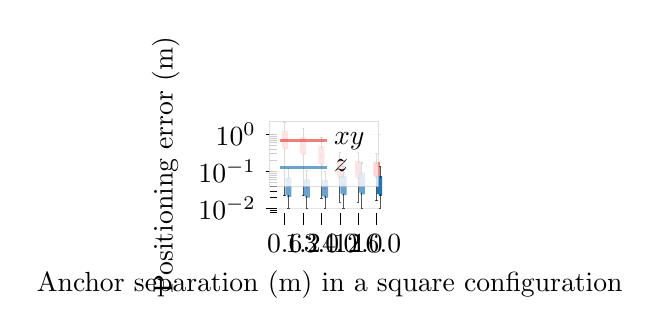
\begin{tikzpicture}

% \definecolor{color0}{rgb}{0.91796875,0.25,0.203125}
% \definecolor{color1}{rgb}{1,0.498039215686275,0.0549019607843137}
% \definecolor{color2}{rgb}{0.6328125,0.203125,0.91796875}

\definecolor{color0}{rgb}{0.91796875,0.25,0.203125}
\definecolor{color1}{rgb}{0.6328125,0.203125,0.91796875}
\definecolor{color2}{rgb}{0.12156862745098,0.466666666666667,0.705882352941177}
\definecolor{color3}{rgb}{0.580392156862745,0.403921568627451,0.741176470588235}
\definecolor{color4}{rgb}{0.890196078431372,0.466666666666667,0.76078431372549}
\definecolor{color5}{rgb}{0.854901960784314,0.647058823529412,0.125490196078431}
\definecolor{color6}{rgb}{0.980392156862745,0.501960784313725,0.447058823529412}
\definecolor{color7}{rgb}{0.627450980392157,0.32156862745098,0.176470588235294}

\begin{axis}[
    height=\figureheight,
    width=\figurewidth,
    axis line style={white},
    tick align=outside,
    tick pos=left,
    x grid style={white!69.0196078431373!black},
    xtick style={color=black},
    y grid style={white!90!black},
    ymajorgrids,
    ytick style={color=black},
    scaled y ticks = false,
    legend cell align={left},
    legend style={
      fill opacity=0.8,
      draw opacity=0.666,
      text opacity=1,
      at={(0.97,0.97)},
      anchor=north east,
      draw=white!80!black
    },
    tick align=outside,
    tick pos=left,
    %
    %
    %
    %
    %
    %
    %
    % legend cell align={left},
    % legend style={fill opacity=0.8, draw opacity=1, text opacity=1, draw=white!80!black},
    log basis y={10},
    % tick align=outside,
    % tick pos=left,
    % title={Navigation error\_s Based on Different Anchor Distributions},
    % x grid style={white!69.0196078431373!black},
    xlabel={Anchor separation (m) in a square configuration},
    xmin=3, xmax=31.5,
    xtick style={color=black},
    xtick={5,10,15,20,25,30},
    xticklabels={0.6, 1.2, 3.0, 4.0, 12.0, 16.0},
    % y grid style={white!69.0196078431373!black},
    ylabel={Positioning error (m)},
    % ymajorgrids,
    ymin=0.00764756728151565, ymax=2.80953482304376,
    ymode=log,
    ytick style={color=black}
]
\addplot [line width=1.2pt, color0, forget plot, fill opacity=0.2, draw opacity=0.666]
table {%
4.625 0.439554516706074
5.375 0.439554516706074
5.375 0.737430373321974
5.3375 0.754528586674168
5.375 0.771626800026362
5.375 1.12453661410266
4.625 1.12453661410266
4.625 0.771626800026362
4.6625 0.754528586674168
4.625 0.737430373321974
4.625 0.439554516706074
};
\addplot [black, forget plot, fill opacity=0.2, draw opacity=0.666]
table {%
5 0.439554516706074
5 0.0220055426779344
};
\addplot [black, forget plot, fill opacity=0.2, draw opacity=0.666]
table {%
5 1.12453661410266
5 2.14802068736096
};
\addplot [black, forget plot, fill opacity=0.2, draw opacity=0.666]
table {%
4.6625 0.0220055426779344
5.3375 0.0220055426779344
};
\addplot [black, forget plot, fill opacity=0.2, draw opacity=0.666]
table {%
4.6625 2.14802068736096
5.3375 2.14802068736096
};
\addplot [line width=1.2pt, color2, forget plot, fill opacity=0.2, draw opacity=0.666]
table {%
5.625 0.0227598094903185
6.375 0.0227598094903185
6.375 0.0376965880679522
6.3375 0.038663463590705
6.375 0.0396303391134579
6.375 0.0614944076529778
5.625 0.0614944076529778
5.625 0.0396303391134579
5.6625 0.038663463590705
5.625 0.0376965880679522
5.625 0.0227598094903185
};
\addplot [black, forget plot, fill opacity=0.2, draw opacity=0.666]
table {%
6 0.0227598094903185
6 0.0100163269011766
};
\addplot [black, forget plot, fill opacity=0.2, draw opacity=0.666]
table {%
6 0.0614944076529778
6 0.119412460327505
};
\addplot [black, forget plot, fill opacity=0.2, draw opacity=0.666]
table {%
5.6625 0.0100163269011766
6.3375 0.0100163269011766
};
\addplot [black, forget plot, fill opacity=0.2, draw opacity=0.666]
table {%
5.6625 0.119412460327505
6.3375 0.119412460327505
};
\addplot [line width=1.2pt, color0, forget plot, fill opacity=0.2, draw opacity=0.666]
table {%
9.625 0.304072100862414
10.375 0.304072100862414
10.375 0.498386030423313
10.3375 0.510222380636263
10.375 0.522058730849214
10.375 0.769545213987761
9.625 0.769545213987761
9.625 0.522058730849214
9.6625 0.510222380636263
9.625 0.498386030423313
9.625 0.304072100862414
};
\addplot [black, forget plot, fill opacity=0.2, draw opacity=0.666]
table {%
10 0.304072100862414
10 0.0218408489867037
};
\addplot [black, forget plot, fill opacity=0.2, draw opacity=0.666]
table {%
10 0.769545213987761
10 1.46399043870141
};
\addplot [black, forget plot, fill opacity=0.2, draw opacity=0.666]
table {%
9.6625 0.0218408489867037
10.3375 0.0218408489867037
};
\addplot [black, forget plot, fill opacity=0.2, draw opacity=0.666]
table {%
9.6625 1.46399043870141
10.3375 1.46399043870141
};
\addplot [line width=1.2pt, color2, forget plot, fill opacity=0.2, draw opacity=0.666]
table {%
10.625 0.0218391990654183
11.375 0.0218391990654183
11.375 0.0351104427052195
11.3375 0.0359444141397498
11.375 0.0367783855742801
11.375 0.054635734560263
10.625 0.054635734560263
10.625 0.0367783855742801
10.6625 0.0359444141397498
10.625 0.0351104427052195
10.625 0.0218391990654183
};
\addplot [black, forget plot, fill opacity=0.2, draw opacity=0.666]
table {%
11 0.0218391990654183
11 0.0100086593626756
};
\addplot [black, forget plot, fill opacity=0.2, draw opacity=0.666]
table {%
11 0.054635734560263
11 0.103695297241881
};
\addplot [black, forget plot, fill opacity=0.2, draw opacity=0.666]
table {%
10.6625 0.0100086593626756
11.3375 0.0100086593626756
};
\addplot [black, forget plot, fill opacity=0.2, draw opacity=0.666]
table {%
10.6625 0.103695297241881
11.3375 0.103695297241881
};
\addplot [line width=1.2pt, color0, forget plot, fill opacity=0.2, draw opacity=0.666]
table {%
14.625 0.160954992029104
15.375 0.160954992029104
15.375 0.269166198619019
15.3375 0.27600872791582
15.375 0.282851257212621
15.375 0.429229443636009
14.625 0.429229443636009
14.625 0.282851257212621
14.6625 0.27600872791582
14.625 0.269166198619019
14.625 0.160954992029104
};
\addplot [black, forget plot, fill opacity=0.2, draw opacity=0.666]
table {%
15 0.160954992029104
15 0.0187509978680707
};
\addplot [black, forget plot, fill opacity=0.2, draw opacity=0.666]
table {%
15 0.429229443636009
15 0.831071782598781
};
\addplot [black, forget plot, fill opacity=0.2, draw opacity=0.666]
table {%
14.6625 0.0187509978680707
15.3375 0.0187509978680707
};
\addplot [black, forget plot, fill opacity=0.2, draw opacity=0.666]
table {%
14.6625 0.831071782598781
15.3375 0.831071782598781
};
\addplot [line width=1.2pt, color2, forget plot, fill opacity=0.2, draw opacity=0.666]
table {%
15.625 0.0216860198958884
16.375 0.0216860198958884
16.375 0.0336951125178267
16.3375 0.0345083618143178
16.375 0.0353216111108089
16.375 0.0535710144019177
15.625 0.0535710144019177
15.625 0.0353216111108089
15.6625 0.0345083618143178
15.625 0.0336951125178267
15.625 0.0216860198958884
};
\addplot [black, forget plot, fill opacity=0.2, draw opacity=0.666]
table {%
16 0.0216860198958884
16 0.010002746582197
};
\addplot [black, forget plot, fill opacity=0.2, draw opacity=0.666]
table {%
16 0.0535710144019177
16 0.101269760134251
};
\addplot [black, forget plot, fill opacity=0.2, draw opacity=0.666]
table {%
15.6625 0.010002746582197
16.3375 0.010002746582197
};
\addplot [black, forget plot, fill opacity=0.2, draw opacity=0.666]
table {%
15.6625 0.101269760134251
16.3375 0.101269760134251
};
\addplot [line width=1.2pt, color0, forget plot, fill opacity=0.2, draw opacity=0.666]
table {%
19.625 0.0743437322548258
20.375 0.0743437322548258
20.375 0.112364838220193
20.3375 0.114852232513715
20.375 0.117339626807236
20.375 0.175182168642137
19.625 0.175182168642137
19.625 0.117339626807236
19.6625 0.114852232513715
19.625 0.112364838220193
19.625 0.0743437322548258
};
\addplot [black, forget plot, fill opacity=0.2, draw opacity=0.666]
table {%
20 0.0743437322548258
20 0.0148281074374566
};
\addplot [black, forget plot, fill opacity=0.2, draw opacity=0.666]
table {%
20 0.175182168642137
20 0.325943142869699
};
\addplot [black, forget plot, fill opacity=0.2, draw opacity=0.666]
table {%
19.6625 0.0148281074374566
20.3375 0.0148281074374566
};
\addplot [black, forget plot, fill opacity=0.2, draw opacity=0.666]
table {%
19.6625 0.325943142869699
20.3375 0.325943142869699
};
\addplot [line width=1.2pt, color2, forget plot, fill opacity=0.2, draw opacity=0.666]
table {%
20.625 0.0252690315248048
21.375 0.0252690315248048
21.375 0.0418912171206516
21.3375 0.0429774475068605
21.375 0.0440636778930694
21.375 0.0693045806884349
20.625 0.0693045806884349
20.625 0.0440636778930694
20.6625 0.0429774475068605
20.625 0.0418912171206516
20.625 0.0252690315248048
};
\addplot [black, forget plot, fill opacity=0.2, draw opacity=0.666]
table {%
21 0.0252690315248048
21 0.0100065231321462
};
\addplot [black, forget plot, fill opacity=0.2, draw opacity=0.666]
table {%
21 0.0693045806884349
21 0.135276498794538
};
\addplot [black, forget plot, fill opacity=0.2, draw opacity=0.666]
table {%
20.6625 0.0100065231321462
21.3375 0.0100065231321462
};
\addplot [black, forget plot, fill opacity=0.2, draw opacity=0.666]
table {%
20.6625 0.135276498794538
21.3375 0.135276498794538
};
\addplot [line width=1.2pt, color0, forget plot, fill opacity=0.2, draw opacity=0.666]
table {%
24.625 0.0701212204465497
25.375 0.0701212204465497
25.375 0.109461681139149
25.3375 0.111868954870416
25.375 0.114276228601684
25.375 0.171550766308991
24.625 0.171550766308991
24.625 0.114276228601684
24.6625 0.111868954870416
24.625 0.109461681139149
24.625 0.0701212204465497
};
\addplot [black, forget plot, fill opacity=0.2, draw opacity=0.666]
table {%
25 0.0701212204465497
25 0.0148874472174385
};
\addplot [black, forget plot, fill opacity=0.2, draw opacity=0.666]
table {%
25 0.171550766308991
25 0.323299778113673
};
\addplot [black, forget plot, fill opacity=0.2, draw opacity=0.666]
table {%
24.6625 0.0148874472174385
25.3375 0.0148874472174385
};
\addplot [black, forget plot, fill opacity=0.2, draw opacity=0.666]
table {%
24.6625 0.323299778113673
25.3375 0.323299778113673
};
\addplot [line width=1.2pt, color2, forget plot, fill opacity=0.2, draw opacity=0.666]
table {%
25.625 0.0268080949799031
26.375 0.0268080949799031
26.375 0.0461058134653612
26.3375 0.0474589157103367
26.375 0.0488120179553121
26.375 0.0838205337527231
25.625 0.0838205337527231
25.625 0.0488120179553121
25.6625 0.0474589157103367
25.625 0.0461058134653612
25.625 0.0268080949799031
};
\addplot [black, forget plot, fill opacity=0.2, draw opacity=0.666]
table {%
26 0.0268080949799031
26 0.0100078964231152
};
\addplot [black, forget plot, fill opacity=0.2, draw opacity=0.666]
table {%
26 0.0838205337527231
26 0.169114484790567
};
\addplot [black, forget plot, fill opacity=0.2, draw opacity=0.666]
table {%
25.6625 0.0100078964231152
26.3375 0.0100078964231152
};
\addplot [black, forget plot, fill opacity=0.2, draw opacity=0.666]
table {%
25.6625 0.169114484790567
26.3375 0.169114484790567
};
\addplot [line width=1.2pt, color0]
table {%
29.625 0.0730683323501405
30.375 0.0730683323501405
30.375 0.108837554707475
30.3375 0.111230971460088
30.375 0.113624388212701
30.375 0.163527312401688
29.625 0.163527312401688
29.625 0.113624388212701
29.6625 0.111230971460088
29.625 0.108837554707475
29.625 0.0730683323501405
};
\addlegendentry{$xy$}
\addplot [black, forget plot, fill opacity=0.2, draw opacity=0.666]
table {%
30 0.0730683323501405
30 0.0161690433533463
};
\addplot [black, forget plot, fill opacity=0.2, draw opacity=0.666]
table {%
30 0.163527312401688
30 0.29891230024487
};
\addplot [black, forget plot, fill opacity=0.2, draw opacity=0.666]
table {%
29.6625 0.0161690433533463
30.3375 0.0161690433533463
};
\addplot [black, forget plot, fill opacity=0.2, draw opacity=0.666]
table {%
29.6625 0.29891230024487
30.3375 0.29891230024487
};
\addplot [line width=1.2pt, color2]
table {%
30.625 0.0243167877202097
31.375 0.0243167877202097
31.375 0.0408140304581669
31.3375 0.0419668579137156
31.375 0.0431196853692642
31.375 0.067887802124833
30.625 0.067887802124833
30.625 0.0431196853692642
30.6625 0.0419668579137156
30.625 0.0408140304581669
30.625 0.0243167877202097
};
\addlegendentry{$z$}
\addplot [black, forget plot, fill opacity=0.2, draw opacity=0.666]
table {%
31 0.0243167877202097
31 0.0100028228787785
};
\addplot [black, forget plot, fill opacity=0.2, draw opacity=0.666]
table {%
31 0.067887802124833
31 0.132734718319185
};
\addplot [black, forget plot, fill opacity=0.2, draw opacity=0.666]
table {%
30.6625 0.0100028228787785
31.3375 0.0100028228787785
};
\addplot [black, forget plot, fill opacity=0.2, draw opacity=0.666]
table {%
30.6625 0.132734718319185
31.3375 0.132734718319185
};
\addplot [color1, forget plot, fill opacity=0.2, draw opacity=0.666]
table {%
4.6625 0.754528586674168
5.3375 0.754528586674168
};
\addplot [color1, forget plot, fill opacity=0.2, draw opacity=0.666]
table {%
5.6625 0.038663463590705
6.3375 0.038663463590705
};
\addplot [color1, forget plot, fill opacity=0.2, draw opacity=0.666]
table {%
9.6625 0.510222380636263
10.3375 0.510222380636263
};
\addplot [color1, forget plot, fill opacity=0.2, draw opacity=0.666]
table {%
10.6625 0.0359444141397498
11.3375 0.0359444141397498
};
\addplot [color1, forget plot, fill opacity=0.2, draw opacity=0.666]
table {%
14.6625 0.27600872791582
15.3375 0.27600872791582
};
\addplot [color1, forget plot, fill opacity=0.2, draw opacity=0.666]
table {%
15.6625 0.0345083618143178
16.3375 0.0345083618143178
};
\addplot [color1, forget plot, fill opacity=0.2, draw opacity=0.666]
table {%
19.6625 0.114852232513715
20.3375 0.114852232513715
};
\addplot [color1, forget plot, fill opacity=0.2, draw opacity=0.666]
table {%
20.6625 0.0429774475068605
21.3375 0.0429774475068605
};
\addplot [color1, forget plot, fill opacity=0.2, draw opacity=0.666]
table {%
24.6625 0.111868954870416
25.3375 0.111868954870416
};
\addplot [color1, forget plot, fill opacity=0.2, draw opacity=0.666]
table {%
25.6625 0.0474589157103367
26.3375 0.0474589157103367
};
\addplot [color1, forget plot, fill opacity=0.2, draw opacity=0.666]
table {%
29.6625 0.111230971460088
30.3375 0.111230971460088
};
\addplot [color1, forget plot, fill opacity=0.2, draw opacity=0.666]
table {%
30.6625 0.0419668579137156
31.3375 0.0419668579137156
};
\end{axis}

\end{tikzpicture}
}
        \caption{Positioning error based on different anchor distribution settings when doing up and down navigation during a vertical flight.}
        \label{fig:up_down_pos}
    \end{subfigure}
    
    \vspace{1em}
    \begin{subfigure}{0.49\textwidth}
        \centering
        \setlength\figureheight{0.42\textwidth}
        \setlength\figurewidth{0.95\textwidth}
        \footnotesize{% This file was created by tikzplotlib v0.59.8.
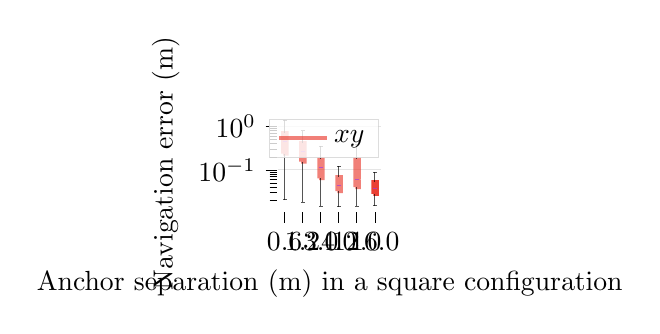
\begin{tikzpicture}

% \definecolor{color0}{rgb}{0.91796875,0.25,0.203125}
% \definecolor{color1}{rgb}{1,0.498039215686275,0.0549019607843137}

\definecolor{color0}{rgb}{0.91796875,0.25,0.203125}
\definecolor{color1}{rgb}{0.6328125,0.203125,0.91796875}
\definecolor{color2}{rgb}{0.12156862745098,0.466666666666667,0.705882352941177}
\definecolor{color3}{rgb}{0.580392156862745,0.403921568627451,0.741176470588235}
\definecolor{color4}{rgb}{0.890196078431372,0.466666666666667,0.76078431372549}
\definecolor{color5}{rgb}{0.854901960784314,0.647058823529412,0.125490196078431}
\definecolor{color6}{rgb}{0.980392156862745,0.501960784313725,0.447058823529412}
\definecolor{color7}{rgb}{0.627450980392157,0.32156862745098,0.176470588235294}

\begin{axis}[
    height=\figureheight,
    width=\figurewidth,
    axis line style={white},
    tick align=outside,
    tick pos=left,
    x grid style={white!69.0196078431373!black},
    xtick style={color=black},
    y grid style={white!90!black},
    ymajorgrids,
    ytick style={color=black},
    scaled y ticks = false,
    legend cell align={left},
    legend style={
      fill opacity=0.8,
      draw opacity=0.666,
      text opacity=1,
      at={(0.97,0.97)},
      anchor=north east,
      draw=white!80!black
    },
    tick align=outside,
    tick pos=left,
    %
    %
    %
    %
    %
    %
    %
    % legend cell align={left},
    % legend style={fill opacity=0.8, draw opacity=1, text opacity=1, draw=white!80!black},
    log basis y={10},
    % tick align=outside,
    % tick pos=left,
    % title={Navigation Errors Based on Different Anchor Distributions},
    % x grid style={white!69.0196078431373!black},
    xlabel={Anchor separation (m) in a square configuration},
    xmin=3, xmax=32,
    % xtick style={color=black},
    xtick={5,10,15,20,25,30},
    xticklabels={0.6, 1.2, 3.0, 4.0, 12.0, 16.0},
    % y grid style={white!69.0196078431373!black},
    ylabel={Navigation error (m)},
    % ymajorgrids,
    ymin=0.0113509597111723, ymax=1.74765612372479,
    ymode=log,
    % ytick style={color=black}
]
\addplot [line width=1.42pt, color0, forget plot, fill opacity=0.2, draw opacity=0.666]
table {%
4.5925 0.236205780787086
5.575 0.236205780787086
5.575 0.434148359697892
5.5375 0.44495072571635
5.575 0.455753091734807
5.575 0.70067693806158
4.5925 0.70067693806158
4.5925 0.455753091734807
4.59625 0.44495072571635
4.5925 0.434148359697892
4.5925 0.236205780787086
};
\addplot [black, forget plot, fill opacity=0.2, draw opacity=0.666]
table {%
5 0.236205780787086
5 0.0206895779141084
};
\addplot [black, forget plot, fill opacity=0.2, draw opacity=0.666]
table {%
5 0.70067693806158
5 1.3900411167484
};
\addplot [black, forget plot, fill opacity=0.2, draw opacity=0.666]
table {%
4.59625 0.0206895779141084
5.5375 0.0206895779141084
};
\addplot [black, forget plot, fill opacity=0.2, draw opacity=0.666]
table {%
4.59625 1.3900411167484
5.5375 1.3900411167484
};
\addplot [line width=1.42pt, color0, forget plot, fill opacity=0.2, draw opacity=0.666]
table {%
9.5925 0.155166271668099
10.575 0.155166271668099
10.575 0.258540842623703
10.5375 0.264733893231419
10.575 0.270926943839134
10.575 0.416108059253237
9.5925 0.416108059253237
9.5925 0.270926943839134
9.59625 0.264733893231419
9.5925 0.258540842623703
9.5925 0.155166271668099
};
\addplot [black, forget plot, fill opacity=0.2, draw opacity=0.666]
table {%
10 0.155166271668099
10 0.0181512185482159
};
\addplot [black, forget plot, fill opacity=0.2, draw opacity=0.666]
table {%
10 0.416108059253237
10 0.807418004645368
};
\addplot [black, forget plot, fill opacity=0.2, draw opacity=0.666]
table {%
9.59625 0.0181512185482159
10.5375 0.0181512185482159
};
\addplot [black, forget plot, fill opacity=0.2, draw opacity=0.666]
table {%
9.59625 0.807418004645368
10.5375 0.807418004645368
};
\addplot [line width=1.42pt, color0, forget plot, fill opacity=0.2, draw opacity=0.666]
table {%
14.5925 0.0642783958570472
15.575 0.0642783958570472
15.575 0.110207956216787
15.5375 0.113027699006243
15.575 0.1158474417957
15.575 0.178024406381381
14.5925 0.178024406381381
14.5925 0.1158474417957
14.59625 0.113027699006243
14.5925 0.110207956216787
14.5925 0.0642783958570472
};
\addplot [black, forget plot, fill opacity=0.2, draw opacity=0.666]
table {%
15 0.0642783958570472
15 0.0145732107322337
};
\addplot [black, forget plot, fill opacity=0.2, draw opacity=0.666]
table {%
15 0.178024406381381
15 0.348616418557662
};
\addplot [black, forget plot, fill opacity=0.2, draw opacity=0.666]
table {%
14.59625 0.0145732107322337
15.5375 0.0145732107322337
};
\addplot [black, forget plot, fill opacity=0.2, draw opacity=0.666]
table {%
14.59625 0.348616418557662
15.5375 0.348616418557662
};
\addplot [line width=1.42pt, color0, forget plot, fill opacity=0.2, draw opacity=0.666]
table {%
19.5925 0.0324889821559235
20.575 0.0324889821559235
20.575 0.0436106794015457
20.5375 0.0446527549668199
20.575 0.0456948305320942
20.575 0.0688315303029189
19.5925 0.0688315303029189
19.5925 0.0456948305320942
19.59625 0.0446527549668199
19.5925 0.0436106794015457
19.5925 0.0324889821559235
};
\addplot [black, forget plot, fill opacity=0.2, draw opacity=0.666]
table {%
20 0.0324889821559235
20 0.014271214002495
};
\addplot [black, forget plot, fill opacity=0.2, draw opacity=0.666]
table {%
20 0.0688315303029189
20 0.121083243093716
};
\addplot [black, forget plot, fill opacity=0.2, draw opacity=0.666]
table {%
19.59625 0.014271214002495
20.5375 0.014271214002495
};
\addplot [black, forget plot, fill opacity=0.2, draw opacity=0.666]
table {%
19.59625 0.121083243093716
20.5375 0.121083243093716
};
\addplot [line width=1.42pt, color0, forget plot, fill opacity=0.2, draw opacity=0.666]
table {%
24.5925 0.0401781042938873
25.575 0.0401781042938873
25.575 0.0571146579117238
25.5375 0.0606484390710363
25.575 0.0641822202303488
25.575 0.177422522725915
24.5925 0.177422522725915
24.5925 0.0641822202303488
24.59625 0.0606484390710363
24.5925 0.0571146579117238
24.5925 0.0401781042938873
};
\addplot [black, forget plot, fill opacity=0.2, draw opacity=0.666]
table {%
25 0.0401781042938873
25 0.0145664257391915
};
\addplot [black, forget plot, fill opacity=0.2, draw opacity=0.666]
table {%
25 0.177422522725915
25 0.382627442819525
};
\addplot [black, forget plot, fill opacity=0.2, draw opacity=0.666]
table {%
24.59625 0.0145664257391915
25.5375 0.0145664257391915
};
\addplot [black, forget plot, fill opacity=0.2, draw opacity=0.666]
table {%
24.59625 0.382627442819525
25.5375 0.382627442819525
};
\addplot [line width=1.42pt, color0]
table {%
29.5925 0.0279812838161758
30.575 0.0279812838161758
30.575 0.0364682033795934
30.5375 0.0372365183562849
30.575 0.0380048333329765
30.575 0.0522533752849953
29.5925 0.0522533752849953
29.5925 0.0380048333329765
29.59625 0.0372365183562849
29.5925 0.0364682033795934
29.5925 0.0279812838161758
};
\addlegendentry{$xy$}
\addplot [black, forget plot, fill opacity=0.2, draw opacity=0.666]
table {%
30 0.0279812838161758
30 0.0151678619195334
};
\addplot [black, forget plot, fill opacity=0.2, draw opacity=0.666]
table {%
30 0.0522533752849953
30 0.0885484219322979
};
\addplot [black, forget plot, fill opacity=0.2, draw opacity=0.666]
table {%
29.59625 0.0151678619195334
30.5375 0.0151678619195334
};
\addplot [black, forget plot, fill opacity=0.2, draw opacity=0.666]
table {%
29.59625 0.0885484219322979
30.5375 0.0885484219322979
};
\addplot [color1, forget plot, fill opacity=0.2, draw opacity=0.666]
table {%
4.59625 0.44495072571635
5.5375 0.44495072571635
};
\addplot [color1, forget plot, fill opacity=0.2, draw opacity=0.666]
table {%
9.59625 0.264733893231419
10.5375 0.264733893231419
};
\addplot [color1, forget plot, fill opacity=0.2, draw opacity=0.666]
table {%
14.59625 0.113027699006243
15.5375 0.113027699006243
};
\addplot [color1, forget plot, fill opacity=0.2, draw opacity=0.666]
table {%
19.59625 0.0446527549668199
20.5375 0.0446527549668199
};
\addplot [color1, forget plot, fill opacity=0.2, draw opacity=0.666]
table {%
24.59625 0.0606484390710363
25.5375 0.0606484390710363
};
\addplot [color1, forget plot, fill opacity=0.2, draw opacity=0.666]
table {%
29.59625 0.0372365183562849
30.5375 0.0372365183562849
};
\end{axis}

\end{tikzpicture}
}
        \caption{Navigation error based on different anchor distribution settings when doing up and down navigation during a vertical flight.}
        \label{fig:up_down_nav}
    \end{subfigure}
    \caption{Positioning and navigation errors over a vertical flight to an altitude of 30\,m. The navigation error includes only the planar distance to the vertical line the drone is set to follow.}
    \label{fig:updown_sim}
\end{figure}

\subsection{Simulation Results}

The positioning and navigation errors for vertical flights are shown in Fig.~\ref{fig:updown_sim}. We observe that the positioning error consistently decreases as the anchors become more separated. For the small UGV setting, the error goes over 1\,m almost 20\% of the time, being highly unstable. It is worth noticing that the navigation error becomes relatively stable with the large UGV anchor distribution (1.2\,m separation). Navigation errors are in general lower than their positioning counterparts as the control of the drone is less affected by individual ranging errors, and these tend to average to zero as time passes. It is also worth noticing that the altitude error is significantly lower in all cases when compared to the planar $xy$ error.

Figure~\ref{fig:square_sim} then shows the results of flights following a square pattern. We can see that if UWB systems based on fixed anchors separated more than 10\,m are utilized, then the navigation error can be consistently maintained below 10\,cm. In the case of relying on small or large UGVs, the error is in the tens of centimeters, providing a competitive alternative to RTK-GNSS systems with higher deployment flexibility and lower system complexity.


% Compare with (0,0)
% %%% up and down navigation errror
% \begin{figure*}
%     \centering
%     \setlength\figureheight{0.33\textwidth}
%     \setlength\figurewidth{\textwidth}
%     \footnotesize{\input{fig/up_down_boxplot_xy}}
%     \caption{Navigation error based on different anchor distribution settings when doing up and down navigation}
%     \label{fig:up_down}
% \end{figure*}

% %%%% Square Positioning
%  \begin{figure*}
%     \centering
%     \setlength\figureheight{0.33\textwidth}
%     \setlength\figurewidth{\textwidth}
%     \footnotesize{\input{fig/square_boxplot_old_data}}
%     % \footnotesize{\input{fig/square_boxplot_old_data}} % before we modified the speed, but looks also good
%     % \footnotesize{\input{fig/square_fig_boxplot}} % Old drawing way
%     \caption{Positioning error based on different anchor distribution settings when doing square navigation at height of 5, 10 and 20 meters}
%     \label{fig:square_position_err}
% \end{figure*}

% %%%% Square Navigation
%  \begin{figure*}
%     \centering
%     \setlength\figureheight{0.33\textwidth}
%     \setlength\figurewidth{\textwidth}
%     \footnotesize{\input{fig/square_fig_boxplot_new}}
%     % \footnotesize{\input{fig/square_navi_boxplot_new_data}} % before we modified the speed, but looks also good
%     % \footnotesize{% This file was created by tikzplotlib v0.9.8.
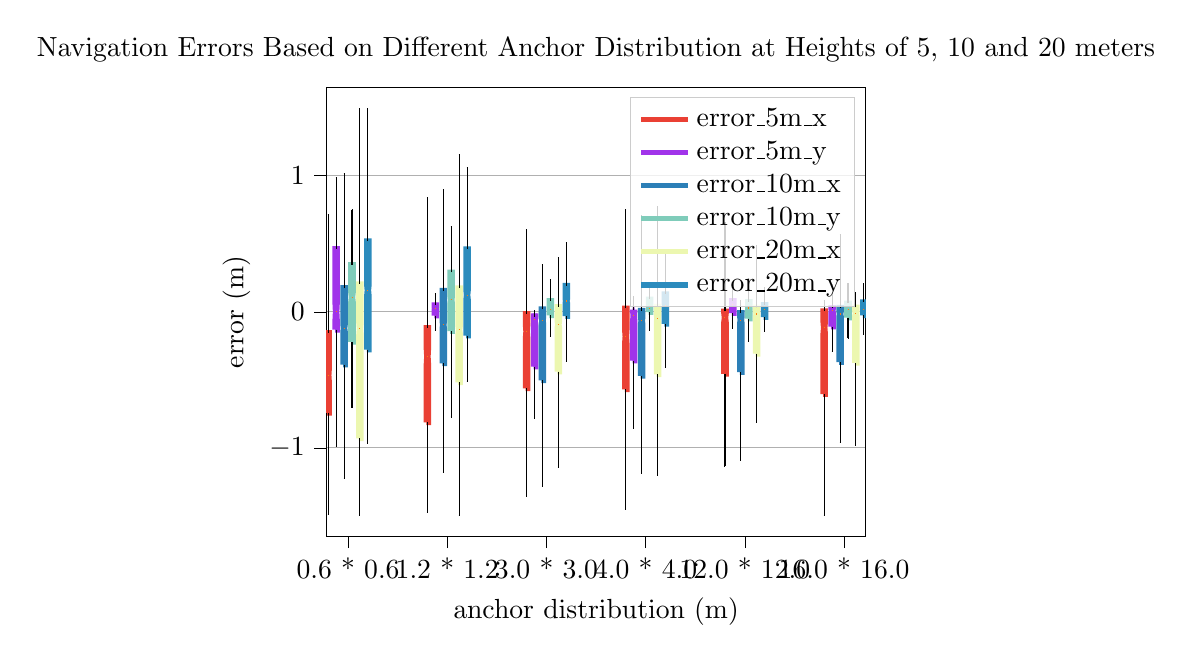
\begin{tikzpicture}

\definecolor{color0}{rgb}{0.91796875,0.25,0.203125}
\definecolor{color1}{rgb}{1,0.498039215686275,0.0549019607843137}
\definecolor{color2}{rgb}{0.6328125,0.203125,0.91796875}
\definecolor{color3}{rgb}{0.171875,0.49609375,0.71875}
\definecolor{color4}{rgb}{0.49609375,0.80078125,0.73046875}
\definecolor{color5}{rgb}{0.92578125,0.96875,0.69140625}
\definecolor{color6}{rgb}{0.16796875,0.546875,0.7421875}

\begin{axis}[
legend cell align={left},
legend style={fill opacity=0.8, draw opacity=1, text opacity=1, draw=white!80!black},
tick align=outside,
tick pos=left,
title={Navigation Errors Based on Different Anchor Distribution at Heights of 5, 10 and 20 meters},
x grid style={white!69.0196078431373!black},
xlabel={anchor distribution (m)},
xmin=4.5, xmax=140.5,
xtick style={color=black},
xtick={10,35,60,85,110,135},
xticklabels={0.6 * 0.6,1.2 * 1.2,3.0 * 3.0,4.0 * 4.0,12.0 * 12.0,16.0 * 16.0},
y grid style={white!69.0196078431373!black},
ylabel={error (m)},
ymajorgrids,
ymin=-1.64954763650894, ymax=1.6459658741951,
ytick style={color=black}
]
\addplot [line width=2pt, color0, forget plot]
table {%
4.75 -0.743499159812927
5.25 -0.743499159812927
5.25 -0.525146243167856
5.125 -0.467144250869751
5.25 -0.409142258571646
5.25 -0.154709577560425
4.75 -0.154709577560425
4.75 -0.409142258571646
4.875 -0.467144250869751
4.75 -0.525146243167856
4.75 -0.743499159812927
};
\addplot [black, forget plot]
table {%
5 -0.743499159812927
5 -1.49304008483887
};
\addplot [black, forget plot]
table {%
5 -0.154709577560425
5 0.718374967575073
};
\addplot [black, forget plot]
table {%
4.875 -1.49304008483887
5.125 -1.49304008483887
};
\addplot [black, forget plot]
table {%
4.875 0.718374967575073
5.125 0.718374967575073
};
\addplot [line width=2pt, color2, forget plot]
table {%
6.75 -0.131946563720703
7.25 -0.131946563720703
7.25 -0.0723783704006997
7.125 0.000148773193359375
7.25 0.0726759167874185
7.25 0.463242530822754
6.75 0.463242530822754
6.75 0.0726759167874185
6.875 0.000148773193359375
6.75 -0.0723783704006997
6.75 -0.131946563720703
};
\addplot [black, forget plot]
table {%
7 -0.131946563720703
7 -0.990792751312256
};
\addplot [black, forget plot]
table {%
7 0.463242530822754
7 0.988891363143921
};
\addplot [black, forget plot]
table {%
6.875 -0.990792751312256
7.125 -0.990792751312256
};
\addplot [black, forget plot]
table {%
6.875 0.988891363143921
7.125 0.988891363143921
};
\addplot [line width=2pt, color3, forget plot]
table {%
8.75 -0.387455701828003
9.25 -0.387455701828003
9.25 -0.147316988453543
9.125 -0.12038254737854
9.25 -0.0934481063035367
9.25 0.176076889038086
8.75 0.176076889038086
8.75 -0.0934481063035367
8.875 -0.12038254737854
8.75 -0.147316988453543
8.75 -0.387455701828003
};
\addplot [black, forget plot]
table {%
9 -0.387455701828003
9 -1.22687864303589
};
\addplot [black, forget plot]
table {%
9 0.176076889038086
9 1.01722145080566
};
\addplot [black, forget plot]
table {%
8.875 -1.22687864303589
9.125 -1.22687864303589
};
\addplot [black, forget plot]
table {%
8.875 1.01722145080566
9.125 1.01722145080566
};
\addplot [line width=2pt, color4, forget plot]
table {%
10.75 -0.221574068069458
11.25 -0.221574068069458
11.25 0.0747884627754247
11.125 0.10714054107666
11.25 0.139492619377896
11.25 0.344258844852448
10.75 0.344258844852448
10.75 0.139492619377896
10.875 0.10714054107666
10.75 0.0747884627754247
10.75 -0.221574068069458
};
\addplot [black, forget plot]
table {%
11 -0.221574068069458
11 -0.703938007354736
};
\addplot [black, forget plot]
table {%
11 0.344258844852448
11 0.747934579849243
};
\addplot [black, forget plot]
table {%
10.875 -0.703938007354736
11.125 -0.703938007354736
};
\addplot [black, forget plot]
table {%
10.875 0.747934579849243
11.125 0.747934579849243
};
\addplot [line width=2pt, color5, forget plot]
table {%
12.75 -0.930796504020691
13.25 -0.930796504020691
13.25 -0.173388450907469
13.125 -0.125516176223755
13.25 -0.0776439015400403
13.25 0.203157663345337
12.75 0.203157663345337
12.75 -0.0776439015400403
12.875 -0.125516176223755
12.75 -0.173388450907469
12.75 -0.930796504020691
};
\addplot [black, forget plot]
table {%
13 -0.930796504020691
13 -1.4982693195343
};
\addplot [black, forget plot]
table {%
13 0.203157663345337
13 1.49449372291565
};
\addplot [black, forget plot]
table {%
12.875 -1.4982693195343
13.125 -1.4982693195343
};
\addplot [black, forget plot]
table {%
12.875 1.49449372291565
13.125 1.49449372291565
};
\addplot [line width=2pt, color6, forget plot]
table {%
14.75 -0.278631925582886
15.25 -0.278631925582886
15.25 0.118936934857174
15.125 0.157839059829712
15.25 0.19674118480225
15.25 0.518910050392151
14.75 0.518910050392151
14.75 0.19674118480225
14.875 0.157839059829712
14.75 0.118936934857174
14.75 -0.278631925582886
};
\addplot [black, forget plot]
table {%
15 -0.278631925582886
15 -0.965609550476074
};
\addplot [black, forget plot]
table {%
15 0.518910050392151
15 1.49616980552673
};
\addplot [black, forget plot]
table {%
14.875 -0.965609550476074
15.125 -0.965609550476074
};
\addplot [black, forget plot]
table {%
14.875 1.49616980552673
15.125 1.49616980552673
};
\addplot [line width=2pt, color0, forget plot]
table {%
29.75 -0.813446998596191
30.25 -0.813446998596191
30.25 -0.394556207424071
30.125 -0.329161167144775
30.25 -0.263766126865479
30.25 -0.117706537246704
29.75 -0.117706537246704
29.75 -0.263766126865479
29.875 -0.329161167144775
29.75 -0.394556207424071
29.75 -0.813446998596191
};
\addplot [black, forget plot]
table {%
30 -0.813446998596191
30 -1.47601437568665
};
\addplot [black, forget plot]
table {%
30 -0.117706537246704
30 0.837147951126099
};
\addplot [black, forget plot]
table {%
29.875 -1.47601437568665
30.125 -1.47601437568665
};
\addplot [black, forget plot]
table {%
29.875 0.837147951126099
30.125 0.837147951126099
};
\addplot [line width=2pt, color2, forget plot]
table {%
31.75 -0.028043270111084
32.25 -0.028043270111084
32.25 0.0124120885327906
32.125 0.0214650630950928
32.25 0.030518037657395
32.25 0.0482367277145386
31.75 0.0482367277145386
31.75 0.030518037657395
31.875 0.0214650630950928
31.75 0.0124120885327906
31.75 -0.028043270111084
};
\addplot [black, forget plot]
table {%
32 -0.028043270111084
32 -0.139469623565674
};
\addplot [black, forget plot]
table {%
32 0.0482367277145386
32 0.13493800163269
};
\addplot [black, forget plot]
table {%
31.875 -0.139469623565674
32.125 -0.139469623565674
};
\addplot [black, forget plot]
table {%
31.875 0.13493800163269
32.125 0.13493800163269
};
\addplot [line width=2pt, color3, forget plot]
table {%
33.75 -0.379667997360229
34.25 -0.379667997360229
34.25 -0.122819693008832
34.125 -0.0961470603942871
34.25 -0.0694744277797426
34.25 0.155146360397339
33.75 0.155146360397339
33.75 -0.0694744277797426
33.875 -0.0961470603942871
33.75 -0.122819693008832
33.75 -0.379667997360229
};
\addplot [black, forget plot]
table {%
34 -0.379667997360229
34 -1.17971181869507
};
\addplot [black, forget plot]
table {%
34 0.155146360397339
34 0.901159763336182
};
\addplot [black, forget plot]
table {%
33.875 -1.17971181869507
34.125 -1.17971181869507
};
\addplot [black, forget plot]
table {%
33.875 0.901159763336182
34.125 0.901159763336182
};
\addplot [line width=2pt, color4, forget plot]
table {%
35.75 -0.141754150390625
36.25 -0.141754150390625
36.25 0.0622168868786168
36.125 0.0872788429260254
36.25 0.112340798973434
36.25 0.289543151855469
35.75 0.289543151855469
35.75 0.112340798973434
35.875 0.0872788429260254
35.75 0.0622168868786168
35.75 -0.141754150390625
};
\addplot [black, forget plot]
table {%
36 -0.141754150390625
36 -0.773646354675293
};
\addplot [black, forget plot]
table {%
36 0.289543151855469
36 0.624154090881348
};
\addplot [black, forget plot]
table {%
35.875 -0.773646354675293
36.125 -0.773646354675293
};
\addplot [black, forget plot]
table {%
35.875 0.624154090881348
36.125 0.624154090881348
};
\addplot [line width=2pt, color5, forget plot]
table {%
37.75 -0.519407749176025
38.25 -0.519407749176025
38.25 -0.163411200467757
38.125 -0.132530212402344
38.25 -0.10164922433693
38.25 0.173223972320557
37.75 0.173223972320557
37.75 -0.10164922433693
37.875 -0.132530212402344
37.75 -0.163411200467757
37.75 -0.519407749176025
};
\addplot [black, forget plot]
table {%
38 -0.519407749176025
38 -1.49975156784058
};
\addplot [black, forget plot]
table {%
38 0.173223972320557
38 1.15402388572693
};
\addplot [black, forget plot]
table {%
37.875 -1.49975156784058
38.125 -1.49975156784058
};
\addplot [black, forget plot]
table {%
37.875 1.15402388572693
38.125 1.15402388572693
};
\addplot [line width=2pt, color6, forget plot]
table {%
39.75 -0.175170183181763
40.25 -0.175170183181763
40.25 0.087918029186913
40.125 0.122923851013184
40.25 0.157929672839454
40.25 0.459796667098999
39.75 0.459796667098999
39.75 0.157929672839454
39.875 0.122923851013184
39.75 0.087918029186913
39.75 -0.175170183181763
};
\addplot [black, forget plot]
table {%
40 -0.175170183181763
40 -0.511089324951172
};
\addplot [black, forget plot]
table {%
40 0.459796667098999
40 1.06014680862427
};
\addplot [black, forget plot]
table {%
39.875 -0.511089324951172
40.125 -0.511089324951172
};
\addplot [black, forget plot]
table {%
39.875 1.06014680862427
40.125 1.06014680862427
};
\addplot [line width=2pt, color0, forget plot]
table {%
54.75 -0.562223672866821
55.25 -0.562223672866821
55.25 -0.193719750303623
55.125 -0.144851922988892
55.25 -0.0959840956741607
55.25 -0.0159645080566406
54.75 -0.0159645080566406
54.75 -0.0959840956741607
54.875 -0.144851922988892
54.75 -0.193719750303623
54.75 -0.562223672866821
};
\addplot [black, forget plot]
table {%
55 -0.562223672866821
55 -1.3540997505188
};
\addplot [black, forget plot]
table {%
55 -0.0159645080566406
55 0.605914115905762
};
\addplot [black, forget plot]
table {%
54.875 -1.3540997505188
55.125 -1.3540997505188
};
\addplot [black, forget plot]
table {%
54.875 0.605914115905762
55.125 0.605914115905762
};
\addplot [line width=2pt, color2, forget plot]
table {%
56.75 -0.403650760650635
57.25 -0.403650760650635
57.25 -0.10487586032227
57.125 -0.0585250854492188
57.25 -0.0121743105761676
57.25 -0.0349112749099731
56.75 -0.0349112749099731
56.75 -0.0121743105761676
56.875 -0.0585250854492188
56.75 -0.10487586032227
56.75 -0.403650760650635
};
\addplot [black, forget plot]
table {%
57 -0.403650760650635
57 -0.786402225494385
};
\addplot [black, forget plot]
table {%
57 -0.0349112749099731
57 0.00796747207641602
};
\addplot [black, forget plot]
table {%
56.875 -0.786402225494385
57.125 -0.786402225494385
};
\addplot [black, forget plot]
table {%
56.875 0.00796747207641602
57.125 0.00796747207641602
};
\addplot [line width=2pt, color3, forget plot]
table {%
58.75 -0.504502773284912
59.25 -0.504502773284912
59.25 -0.0904628306518566
59.125 -0.0640738010406494
59.25 -0.0376847714294423
59.25 0.0192584991455078
58.75 0.0192584991455078
58.75 -0.0376847714294423
58.875 -0.0640738010406494
58.75 -0.0904628306518566
58.75 -0.504502773284912
};
\addplot [black, forget plot]
table {%
59 -0.504502773284912
59 -1.28569006919861
};
\addplot [black, forget plot]
table {%
59 0.0192584991455078
59 0.349289417266846
};
\addplot [black, forget plot]
table {%
58.875 -1.28569006919861
59.125 -1.28569006919861
};
\addplot [black, forget plot]
table {%
58.875 0.349289417266846
59.125 0.349289417266846
};
\addplot [line width=2pt, color4, forget plot]
table {%
60.75 -0.0260365009307861
61.25 -0.0260365009307861
61.25 0.00821392658492199
61.125 0.0144844055175781
61.25 0.0207548844502343
61.25 0.0809085369110107
60.75 0.0809085369110107
60.75 0.0207548844502343
60.875 0.0144844055175781
60.75 0.00821392658492199
60.75 -0.0260365009307861
};
\addplot [black, forget plot]
table {%
61 -0.0260365009307861
61 -0.183313846588135
};
\addplot [black, forget plot]
table {%
61 0.0809085369110107
61 0.239443302154541
};
\addplot [black, forget plot]
table {%
60.875 -0.183313846588135
61.125 -0.183313846588135
};
\addplot [black, forget plot]
table {%
60.875 0.239443302154541
61.125 0.239443302154541
};
\addplot [line width=2pt, color5, forget plot]
table {%
62.75 -0.440536379814148
63.25 -0.440536379814148
63.25 -0.117323998207768
63.125 -0.0936794281005859
63.25 -0.0700348579934036
63.25 0.0361860990524292
62.75 0.0361860990524292
62.75 -0.0700348579934036
62.875 -0.0936794281005859
62.75 -0.117323998207768
62.75 -0.440536379814148
};
\addplot [black, forget plot]
table {%
63 -0.440536379814148
63 -1.14689373970032
};
\addplot [black, forget plot]
table {%
63 0.0361860990524292
63 0.39593243598938
};
\addplot [black, forget plot]
table {%
62.875 -1.14689373970032
63.125 -1.14689373970032
};
\addplot [black, forget plot]
table {%
62.875 0.39593243598938
63.125 0.39593243598938
};
\addplot [line width=2pt, color6, forget plot]
table {%
64.75 -0.0323653221130371
65.25 -0.0323653221130371
65.25 0.0660148612849231
65.125 0.079188346862793
65.25 0.0923618324406628
65.25 0.192312717437744
64.75 0.192312717437744
64.75 0.0923618324406628
64.875 0.079188346862793
64.75 0.0660148612849231
64.75 -0.0323653221130371
};
\addplot [black, forget plot]
table {%
65 -0.0323653221130371
65 -0.36549186706543
};
\addplot [black, forget plot]
table {%
65 0.192312717437744
65 0.507901668548584
};
\addplot [black, forget plot]
table {%
64.875 -0.36549186706543
65.125 -0.36549186706543
};
\addplot [black, forget plot]
table {%
64.875 0.507901668548584
65.125 0.507901668548584
};
\addplot [line width=2pt, color0, forget plot]
table {%
79.75 -0.569836616516113
80.25 -0.569836616516113
80.25 -0.235042256962049
80.125 -0.182058095932007
80.25 -0.129073934901965
80.25 0.0243560075759888
79.75 0.0243560075759888
79.75 -0.129073934901965
79.875 -0.182058095932007
79.75 -0.235042256962049
79.75 -0.569836616516113
};
\addplot [black, forget plot]
table {%
80 -0.569836616516113
80 -1.45652055740356
};
\addplot [black, forget plot]
table {%
80 0.0243560075759888
80 0.749740362167358
};
\addplot [black, forget plot]
table {%
79.875 -1.45652055740356
80.125 -1.45652055740356
};
\addplot [black, forget plot]
table {%
79.875 0.749740362167358
80.125 0.749740362167358
};
\addplot [line width=2pt, color2, forget plot]
table {%
81.75 -0.358523368835449
82.25 -0.358523368835449
82.25 -0.074407939360692
82.125 -0.0296831130981445
82.25 0.0150417131644029
82.25 0.0118095874786377
81.75 0.0118095874786377
81.75 0.0150417131644029
81.875 -0.0296831130981445
81.75 -0.074407939360692
81.75 -0.358523368835449
};
\addplot [black, forget plot]
table {%
82 -0.358523368835449
82 -0.860898017883301
};
\addplot [black, forget plot]
table {%
82 0.0118095874786377
82 0.109017133712769
};
\addplot [black, forget plot]
table {%
81.875 -0.860898017883301
82.125 -0.860898017883301
};
\addplot [black, forget plot]
table {%
81.875 0.109017133712769
82.125 0.109017133712769
};
\addplot [line width=2pt, color3, forget plot]
table {%
83.75 -0.471809029579163
84.25 -0.471809029579163
84.25 -0.0896691022196283
84.125 -0.0663046836853027
84.25 -0.0429402651509771
84.25 0.00765275955200195
83.75 0.00765275955200195
83.75 -0.0429402651509771
83.875 -0.0663046836853027
83.75 -0.0896691022196283
83.75 -0.471809029579163
};
\addplot [black, forget plot]
table {%
84 -0.471809029579163
84 -1.19010138511658
};
\addplot [black, forget plot]
table {%
84 0.00765275955200195
84 0.707371473312378
};
\addplot [black, forget plot]
table {%
83.875 -1.19010138511658
84.125 -1.19010138511658
};
\addplot [black, forget plot]
table {%
83.875 0.707371473312378
84.125 0.707371473312378
};
\addplot [line width=2pt, color4, forget plot]
table {%
85.75 -0.00255393981933594
86.25 -0.00255393981933594
86.25 0.0210572054574293
86.125 0.026512622833252
86.25 0.0319680402090746
86.25 0.0913939476013184
85.75 0.0913939476013184
85.75 0.0319680402090746
85.875 0.026512622833252
85.75 0.0210572054574293
85.75 -0.00255393981933594
};
\addplot [black, forget plot]
table {%
86 -0.00255393981933594
86 -0.137272834777832
};
\addplot [black, forget plot]
table {%
86 0.0913939476013184
86 0.217233657836914
};
\addplot [black, forget plot]
table {%
85.875 -0.137272834777832
86.125 -0.137272834777832
};
\addplot [black, forget plot]
table {%
85.875 0.217233657836914
86.125 0.217233657836914
};
\addplot [line width=2pt, color5, forget plot]
table {%
87.75 -0.459343194961548
88.25 -0.459343194961548
88.25 -0.0741895881550056
88.125 -0.0510034561157227
88.25 -0.0278173240764397
88.25 0.0386333465576172
87.75 0.0386333465576172
87.75 -0.0278173240764397
87.875 -0.0510034561157227
87.75 -0.0741895881550056
87.75 -0.459343194961548
};
\addplot [black, forget plot]
table {%
88 -0.459343194961548
88 -1.20585107803345
};
\addplot [black, forget plot]
table {%
88 0.0386333465576172
88 0.775400161743164
};
\addplot [black, forget plot]
table {%
87.875 -1.20585107803345
88.125 -1.20585107803345
};
\addplot [black, forget plot]
table {%
87.875 0.775400161743164
88.125 0.775400161743164
};
\addplot [line width=2pt, color6, forget plot]
table {%
89.75 -0.0880992412567139
90.25 -0.0880992412567139
90.25 0.0303827887566641
90.125 0.0431675910949707
90.25 0.0559523934332773
90.25 0.130557060241699
89.75 0.130557060241699
89.75 0.0559523934332773
89.875 0.0431675910949707
89.75 0.0303827887566641
89.75 -0.0880992412567139
};
\addplot [black, forget plot]
table {%
90 -0.0880992412567139
90 -0.409366130828857
};
\addplot [black, forget plot]
table {%
90 0.130557060241699
90 0.455041885375977
};
\addplot [black, forget plot]
table {%
89.875 -0.409366130828857
90.125 -0.409366130828857
};
\addplot [black, forget plot]
table {%
89.875 0.455041885375977
90.125 0.455041885375977
};
\addplot [line width=2pt, color0, forget plot]
table {%
104.75 -0.455875158309937
105.25 -0.455875158309937
105.25 -0.075021319219236
105.125 -0.043515682220459
105.25 -0.012010045221682
105.25 0.00216913223266602
104.75 0.00216913223266602
104.75 -0.012010045221682
104.875 -0.043515682220459
104.75 -0.075021319219236
104.75 -0.455875158309937
};
\addplot [black, forget plot]
table {%
105 -0.455875158309937
105 -1.13335347175598
};
\addplot [black, forget plot]
table {%
105 0.00216913223266602
105 0.659635066986084
};
\addplot [black, forget plot]
table {%
104.875 -1.13335347175598
105.125 -1.13335347175598
};
\addplot [black, forget plot]
table {%
104.875 0.659635066986084
105.125 0.659635066986084
};
\addplot [line width=2pt, color2, forget plot]
table {%
106.75 -0.0105390548706055
107.25 -0.0105390548706055
107.25 0.0429628990366717
107.125 0.0507221221923828
107.25 0.0584813453480939
107.25 0.0805902481079102
106.75 0.0805902481079102
106.75 0.0584813453480939
106.875 0.0507221221923828
106.75 0.0429628990366717
106.75 -0.0105390548706055
};
\addplot [black, forget plot]
table {%
107 -0.0105390548706055
107 -0.122659206390381
};
\addplot [black, forget plot]
table {%
107 0.0805902481079102
107 0.198819637298584
};
\addplot [black, forget plot]
table {%
106.875 -0.122659206390381
107.125 -0.122659206390381
};
\addplot [black, forget plot]
table {%
106.875 0.198819637298584
107.125 0.198819637298584
};
\addplot [line width=2pt, color3, forget plot]
table {%
108.75 -0.444120407104492
109.25 -0.444120407104492
109.25 -0.0827250358484453
109.125 -0.0610518455505371
109.25 -0.0393786552526289
109.25 -0.00845521688461304
108.75 -0.00845521688461304
108.75 -0.0393786552526289
108.875 -0.0610518455505371
108.75 -0.0827250358484453
108.75 -0.444120407104492
};
\addplot [black, forget plot]
table {%
109 -0.444120407104492
109 -1.09142136573792
};
\addplot [black, forget plot]
table {%
109 -0.00845521688461304
109 0.0827476978302002
};
\addplot [black, forget plot]
table {%
108.875 -1.09142136573792
109.125 -1.09142136573792
};
\addplot [black, forget plot]
table {%
108.875 0.0827476978302002
109.125 0.0827476978302002
};
\addplot [line width=2pt, color4, forget plot]
table {%
110.75 -0.0497373938560486
111.25 -0.0497373938560486
111.25 0.0210380209799905
111.125 0.0282549858093262
111.25 0.0354719506386618
111.25 0.0727479457855225
110.75 0.0727479457855225
110.75 0.0354719506386618
110.875 0.0282549858093262
110.75 0.0210380209799905
110.75 -0.0497373938560486
};
\addplot [black, forget plot]
table {%
111 -0.0497373938560486
111 -0.215531826019287
};
\addplot [black, forget plot]
table {%
111 0.0727479457855225
111 0.246762752532959
};
\addplot [black, forget plot]
table {%
110.875 -0.215531826019287
111.125 -0.215531826019287
};
\addplot [black, forget plot]
table {%
110.875 0.246762752532959
111.125 0.246762752532959
};
\addplot [line width=2pt, color5, forget plot]
table {%
112.75 -0.308400630950928
113.25 -0.308400630950928
113.25 -0.0320072243321562
113.125 -0.0163217782974243
113.25 -0.000636332262692392
113.25 0.0327502489089966
112.75 0.0327502489089966
112.75 -0.000636332262692392
112.875 -0.0163217782974243
112.75 -0.0320072243321562
112.75 -0.308400630950928
};
\addplot [black, forget plot]
table {%
113 -0.308400630950928
113 -0.810099363327026
};
\addplot [black, forget plot]
table {%
113 0.0327502489089966
113 0.48962664604187
};
\addplot [black, forget plot]
table {%
112.875 -0.810099363327026
113.125 -0.810099363327026
};
\addplot [black, forget plot]
table {%
112.875 0.48962664604187
113.125 0.48962664604187
};
\addplot [line width=2pt, color6, forget plot]
table {%
114.75 -0.0387712717056274
115.25 -0.0387712717056274
115.25 0.00898072605497949
115.125 0.0143465995788574
115.25 0.0197124731027354
115.25 0.0510708093643188
114.75 0.0510708093643188
114.75 0.0197124731027354
114.875 0.0143465995788574
114.75 0.00898072605497949
114.75 -0.0387712717056274
};
\addplot [black, forget plot]
table {%
115 -0.0387712717056274
115 -0.148081302642822
};
\addplot [black, forget plot]
table {%
115 0.0510708093643188
115 0.178939819335938
};
\addplot [black, forget plot]
table {%
114.875 -0.148081302642822
115.125 -0.148081302642822
};
\addplot [black, forget plot]
table {%
114.875 0.178939819335938
115.125 0.178939819335938
};
\addplot [line width=2pt, color0]
table {%
129.75 -0.605347871780396
130.25 -0.605347871780396
130.25 -0.164041313691595
130.125 -0.118365287780762
130.25 -0.0726892618699287
130.25 0.00491225719451904
129.75 0.00491225719451904
129.75 -0.0726892618699287
129.875 -0.118365287780762
129.75 -0.164041313691595
129.75 -0.605347871780396
};
\addlegendentry{error\_5m\_x}
\addplot [black, forget plot]
table {%
130 -0.605347871780396
130 -1.49771499633789
};
\addplot [black, forget plot]
table {%
130 0.00491225719451904
130 0.0810000896453857
};
\addplot [black, forget plot]
table {%
129.875 -1.49771499633789
130.125 -1.49771499633789
};
\addplot [black, forget plot]
table {%
129.875 0.0810000896453857
130.125 0.0810000896453857
};
\addplot [line width=2pt, color2]
table {%
131.75 -0.109168529510498
132.25 -0.109168529510498
132.25 -0.00628540810040713
132.125 0.00816845893859863
132.25 0.0226223259776044
132.25 0.0280020236968994
131.75 0.0280020236968994
131.75 0.0226223259776044
131.875 0.00816845893859863
131.75 -0.00628540810040713
131.75 -0.109168529510498
};
\addlegendentry{error\_5m\_y}
\addplot [black, forget plot]
table {%
132 -0.109168529510498
132 -0.290670394897461
};
\addplot [black, forget plot]
table {%
132 0.0280020236968994
132 0.196889400482178
};
\addplot [black, forget plot]
table {%
131.875 -0.290670394897461
132.125 -0.290670394897461
};
\addplot [black, forget plot]
table {%
131.875 0.196889400482178
132.125 0.196889400482178
};
\addplot [line width=2pt, color3]
table {%
133.75 -0.369070529937744
134.25 -0.369070529937744
134.25 -0.0349901813530299
134.125 -0.0160374641418457
134.25 0.0029152530693385
134.25 0.0298470258712769
133.75 0.0298470258712769
133.75 0.0029152530693385
133.875 -0.0160374641418457
133.75 -0.0349901813530299
133.75 -0.369070529937744
};
\addlegendentry{error\_10m\_x}
\addplot [black, forget plot]
table {%
134 -0.369070529937744
134 -0.963465213775635
};
\addplot [black, forget plot]
table {%
134 0.0298470258712769
134 0.568765163421631
};
\addplot [black, forget plot]
table {%
133.875 -0.963465213775635
134.125 -0.963465213775635
};
\addplot [black, forget plot]
table {%
133.875 0.568765163421631
134.125 0.568765163421631
};
\addplot [line width=2pt, color4]
table {%
135.75 -0.0430431365966797
136.25 -0.0430431365966797
136.25 0.0105473146886084
136.125 0.0169897079467773
136.25 0.0234321012049463
136.25 0.0623760223388672
135.75 0.0623760223388672
135.75 0.0234321012049463
135.875 0.0169897079467773
135.75 0.0105473146886084
135.75 -0.0430431365966797
};
\addlegendentry{error\_10m\_y}
\addplot [black, forget plot]
table {%
136 -0.0430431365966797
136 -0.194686412811279
};
\addplot [black, forget plot]
table {%
136 0.0623760223388672
136 0.208606243133545
};
\addplot [black, forget plot]
table {%
135.875 -0.194686412811279
136.125 -0.194686412811279
};
\addplot [black, forget plot]
table {%
135.875 0.208606243133545
136.125 0.208606243133545
};
\addplot [line width=2pt, color5]
table {%
137.75 -0.374789237976074
138.25 -0.374789237976074
138.25 -0.0313415219239674
138.125 -0.0123014450073242
138.25 0.00673863190931901
138.25 0.0328803062438965
137.75 0.0328803062438965
137.75 0.00673863190931901
137.875 -0.0123014450073242
137.75 -0.0313415219239674
137.75 -0.374789237976074
};
\addlegendentry{error\_20m\_x}
\addplot [black, forget plot]
table {%
138 -0.374789237976074
138 -0.983993291854858
};
\addplot [black, forget plot]
table {%
138 0.0328803062438965
138 0.140230417251587
};
\addplot [black, forget plot]
table {%
137.875 -0.983993291854858
138.125 -0.983993291854858
};
\addplot [black, forget plot]
table {%
137.875 0.140230417251587
138.125 0.140230417251587
};
\addplot [line width=2pt, color6]
table {%
139.75 -0.0257692337036133
140.25 -0.0257692337036133
140.25 0.0111079485687032
140.125 0.0168507099151611
140.25 0.0225934712616191
140.25 0.0701742172241211
139.75 0.0701742172241211
139.75 0.0225934712616191
139.875 0.0168507099151611
139.75 0.0111079485687032
139.75 -0.0257692337036133
};
\addlegendentry{error\_20m\_y}
\addplot [black, forget plot]
table {%
140 -0.0257692337036133
140 -0.168480396270752
};
\addplot [black, forget plot]
table {%
140 0.0701742172241211
140 0.209501266479492
};
\addplot [black, forget plot]
table {%
139.875 -0.168480396270752
140.125 -0.168480396270752
};
\addplot [black, forget plot]
table {%
139.875 0.209501266479492
140.125 0.209501266479492
};
\addplot [color1, forget plot]
table {%
4.875 -0.467144250869751
5.125 -0.467144250869751
};
\addplot [color1, forget plot]
table {%
6.875 0.000148773193359375
7.125 0.000148773193359375
};
\addplot [color1, forget plot]
table {%
8.875 -0.12038254737854
9.125 -0.12038254737854
};
\addplot [color1, forget plot]
table {%
10.875 0.10714054107666
11.125 0.10714054107666
};
\addplot [color1, forget plot]
table {%
12.875 -0.125516176223755
13.125 -0.125516176223755
};
\addplot [color1, forget plot]
table {%
14.875 0.157839059829712
15.125 0.157839059829712
};
\addplot [color1, forget plot]
table {%
29.875 -0.329161167144775
30.125 -0.329161167144775
};
\addplot [color1, forget plot]
table {%
31.875 0.0214650630950928
32.125 0.0214650630950928
};
\addplot [color1, forget plot]
table {%
33.875 -0.0961470603942871
34.125 -0.0961470603942871
};
\addplot [color1, forget plot]
table {%
35.875 0.0872788429260254
36.125 0.0872788429260254
};
\addplot [color1, forget plot]
table {%
37.875 -0.132530212402344
38.125 -0.132530212402344
};
\addplot [color1, forget plot]
table {%
39.875 0.122923851013184
40.125 0.122923851013184
};
\addplot [color1, forget plot]
table {%
54.875 -0.144851922988892
55.125 -0.144851922988892
};
\addplot [color1, forget plot]
table {%
56.875 -0.0585250854492188
57.125 -0.0585250854492188
};
\addplot [color1, forget plot]
table {%
58.875 -0.0640738010406494
59.125 -0.0640738010406494
};
\addplot [color1, forget plot]
table {%
60.875 0.0144844055175781
61.125 0.0144844055175781
};
\addplot [color1, forget plot]
table {%
62.875 -0.0936794281005859
63.125 -0.0936794281005859
};
\addplot [color1, forget plot]
table {%
64.875 0.079188346862793
65.125 0.079188346862793
};
\addplot [color1, forget plot]
table {%
79.875 -0.182058095932007
80.125 -0.182058095932007
};
\addplot [color1, forget plot]
table {%
81.875 -0.0296831130981445
82.125 -0.0296831130981445
};
\addplot [color1, forget plot]
table {%
83.875 -0.0663046836853027
84.125 -0.0663046836853027
};
\addplot [color1, forget plot]
table {%
85.875 0.026512622833252
86.125 0.026512622833252
};
\addplot [color1, forget plot]
table {%
87.875 -0.0510034561157227
88.125 -0.0510034561157227
};
\addplot [color1, forget plot]
table {%
89.875 0.0431675910949707
90.125 0.0431675910949707
};
\addplot [color1, forget plot]
table {%
104.875 -0.043515682220459
105.125 -0.043515682220459
};
\addplot [color1, forget plot]
table {%
106.875 0.0507221221923828
107.125 0.0507221221923828
};
\addplot [color1, forget plot]
table {%
108.875 -0.0610518455505371
109.125 -0.0610518455505371
};
\addplot [color1, forget plot]
table {%
110.875 0.0282549858093262
111.125 0.0282549858093262
};
\addplot [color1, forget plot]
table {%
112.875 -0.0163217782974243
113.125 -0.0163217782974243
};
\addplot [color1, forget plot]
table {%
114.875 0.0143465995788574
115.125 0.0143465995788574
};
\addplot [color1, forget plot]
table {%
129.875 -0.118365287780762
130.125 -0.118365287780762
};
\addplot [color1, forget plot]
table {%
131.875 0.00816845893859863
132.125 0.00816845893859863
};
\addplot [color1, forget plot]
table {%
133.875 -0.0160374641418457
134.125 -0.0160374641418457
};
\addplot [color1, forget plot]
table {%
135.875 0.0169897079467773
136.125 0.0169897079467773
};
\addplot [color1, forget plot]
table {%
137.875 -0.0123014450073242
138.125 -0.0123014450073242
};
\addplot [color1, forget plot]
table {%
139.875 0.0168507099151611
140.125 0.0168507099151611
};
\end{axis}

\end{tikzpicture}
} % Old drawing way
%     \caption{Navigation error based on different anchor distribution settings when doing square navigation at height of 5, 10 and 20 meters}
%     \label{fig:square_position_err}
% \end{figure*}



%  \begin{figure*}
%     \centering
%     \setlength\figureheight{0.33\textwidth}
%     \setlength\figurewidth{\textwidth}
%     \footnotesize{\input{fig/square_traj}}
%     \caption{Trajectories based on uwb positioning at the height of 20m}
%     \label{fig:square_all_together}
% \end{figure*}


%  \begin{figure*}
%     \centering
%     \setlength\figureheight{0.33\textwidth}
%     \setlength\figurewidth{\textwidth}
%     \footnotesize{\input{fig/square_fig_boxplot}}
%     \caption{Coordinates positioning error based on different anchor distribution settings when doing square navigation at height of 5, 10 and 20 meters}
%     \label{fig:square_all_heights}
% \end{figure*}


\begin{figure}
    \centering
    \includegraphics[width=0.49\textwidth]{fig/3d_trajectory.png}
    \caption{Partial trajectory of the UAV during the outdoors experiment. VIO is not included because it becomes unusable once the UAV reaches 8\,m of altitude.}
    \label{fig:trajectory}
\end{figure}


\begin{figure}
    \centering
    \setlength\figureheight{0.42\textwidth}
    \setlength\figurewidth{0.49\textwidth}
    \scriptsize{% This file was created by tikzplotlib v0.9.8.
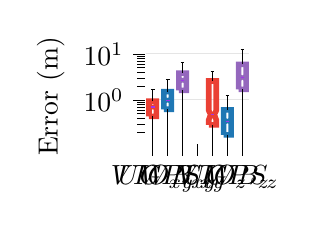
\begin{tikzpicture}

% \definecolor{color0}{rgb}{1,0.498039215686275,0.0549019607843137}
\definecolor{color0}{rgb}{0.91796875,0.25,0.203125}
\definecolor{color1}{rgb}{0.6328125,0.203125,0.91796875}
\definecolor{color2}{rgb}{0.12156862745098,0.466666666666667,0.705882352941177}
\definecolor{color3}{rgb}{0.580392156862745,0.403921568627451,0.741176470588235}
\definecolor{color4}{rgb}{0.890196078431372,0.466666666666667,0.76078431372549}
% \definecolor{color5}{rgb}{0.854901960784314,0.647058823529412,0.125490196078431}
% \definecolor{color6}{rgb}{0.980392156862745,0.501960784313725,0.447058823529412}
% \definecolor{color7}{rgb}{0.627450980392157,0.32156862745098,0.176470588235294}

\definecolor{color7}{rgb}{0.580392156862745,0.403921568627451,0.741176470588235}
\definecolor{color6}{rgb}{0.12156862745098,0.466666666666667,0.705882352941177}
\definecolor{color5}{rgb}{0.91796875,0.25,0.203125}

\begin{axis}[
    height=\figureheight,
    width=\figurewidth,
    axis line style={white},
    tick align=outside,
    tick pos=left,
    x grid style={white!69.0196078431373!black},
    xtick style={color=black},
    y grid style={white!90!black},
    ymajorgrids,
    ytick style={color=black},
    scaled y ticks = false,
    legend cell align={left},
    legend style={
      fill opacity=0.8,
      draw opacity=0.666,
      text opacity=1,
      at={(0.97,0.97)},
      anchor=north east,
      draw=white!80!black
    },
    tick align=outside,
    tick pos=left,
    %
    %
    %
    %
    %
    %
    %
    % legend style={fill opacity=0.8, draw opacity=1, text opacity=1, draw=white!80!black},
    % tick align=outside,
    % tick pos=left,
    % x grid style={white!69.0196078431373!black},
    xmin=0.5, xmax=7.5,
    % xtick style={color=black},
    xtick={1,2,3,4,5,6,7},
    xticklabels={$VIO_{xy}$, $UWB_{xy}$, $GPS_{xy}$, , $VIO_z$, $UWB_z$, $GPS_z$},
    % y grid style={white!69.0196078431373!black},
    ylabel={Error (m)},
    ymajorgrids,
    ymin=0.110018668126381, ymax=12.822998030654,
    ymode=log,
    % ytick style={color=black}
]
\addplot [line width=2pt, color0, forget plot]
table {%
0.75 0.438256200984864
1.25 0.438256200984864
1.25 0.674593597279193
1.125 0.698461927361191
1.25 0.722330257443189
1.25 0.940177507410002
0.75 0.940177507410002
0.75 0.722330257443189
0.875 0.698461927361191
0.75 0.674593597279193
0.75 0.438256200984864
};
% \addlegendentry{VIO}
\addplot [black, forget plot]
table {%
1 0.438256200984864
1 0.0632751893602295
};
\addplot [black, forget plot]
table {%
1 0.940177507410002
1 1.69229048091101
};
\addplot [black, forget plot]
table {%
0.875 0.0632751893602295
1.125 0.0632751893602295
};
\addplot [black, forget plot]
table {%
0.875 1.69229048091101
1.125 1.69229048091101
};
% \addlegendentry{UWB}
\addplot [line width=2pt, color2, forget plot]
table {%
1.75 0.623723617389486
2.25 0.623723617389486
2.25 0.939113143679274
2.125 0.981610969574021
2.25 1.02410879546877
2.25 1.50084906283514
1.75 1.50084906283514
1.75 1.02410879546877
1.875 0.981610969574021
1.75 0.939113143679274
1.75 0.623723617389486
};
\addplot [black, forget plot]
table {%
2 0.623723617389486
2 0.0267978777144759
};
\addplot [black, forget plot]
table {%
2 1.50084906283514
2 2.79929851920673
};
\addplot [black, forget plot]
table {%
1.875 0.0267978777144759
2.125 0.0267978777144759
};
\addplot [black, forget plot]
table {%
1.875 2.79929851920673
2.125 2.79929851920673
};
\addplot [line width=2pt, color3, forget plot]
table {%
2.75 1.60703157784121
3.25 1.60703157784121
3.25 2.55844096266862
3.125 2.6658632409173
3.25 2.77328551916597
3.25 3.8241523758089
2.75 3.8241523758089
2.75 2.77328551916597
2.875 2.6658632409173
2.75 2.55844096266862
2.75 1.60703157784121
};
\addplot [black, forget plot]
table {%
3 1.60703157784121
3 0.0147874407403017
};
\addplot [black, forget plot]
table {%
3 3.8241523758089
3 6.51091049405551
};
\addplot [black, forget plot]
table {%
2.875 0.0147874407403017
3.125 0.0147874407403017
};
\addplot [black, forget plot]
table {%
2.875 6.51091049405551
3.125 6.51091049405551
};
\addplot [line width=2pt, color4, forget plot]
table {%
3.75 nan
4.25 nan
4.25 nan
4.125 nan
4.25 nan
4.25 nan
3.75 nan
3.75 nan
3.875 nan
3.75 nan
3.75 nan
};
\addplot [black, forget plot]
table {%
4 nan
4 nan
};
\addplot [black, forget plot]
table {%
4 nan
4 nan
};
\addplot [black, forget plot]
table {%
3.875 nan
4.125 nan
};
\addplot [black, forget plot]
table {%
3.875 nan
4.125 nan
};
\addplot [line width=2pt, color5, forget plot]
table {%
4.75 0.2863183199475
5.25 0.2863183199475
5.25 0.366798369904502
5.125 0.47536206777
5.25 0.583925765635498
5.25 2.5692779101575
4.75 2.5692779101575
4.75 0.583925765635498
4.875 0.47536206777
4.75 0.366798369904502
4.75 0.2863183199475
};
\addplot [black, forget plot]
table {%
5 0.2863183199475
5 0.0066105721099996
};
\addplot [black, forget plot]
table {%
5 2.5692779101575
5 4.08462203046
};
\addplot [black, forget plot]
table {%
4.875 0.0066105721099996
5.125 0.0066105721099996
};
\addplot [black, forget plot]
table {%
4.875 4.08462203046
5.125 4.08462203046
};
\addplot [line width=2pt, color6, forget plot]
table {%
5.75 0.17235825
6.25 0.17235825
6.25 0.324021683390278
6.125 0.344904499999998
6.25 0.365787316609718
6.25 0.603364999999999
5.75 0.603364999999999
5.75 0.365787316609718
5.875 0.344904499999998
5.75 0.324021683390278
5.75 0.17235825
};
\addplot [black, forget plot]
table {%
6 0.17235825
6 0.000573000000000157
};
\addplot [black, forget plot]
table {%
6 0.603364999999999
6 1.249623
};
\addplot [black, forget plot]
table {%
5.875 0.000573000000000157
6.125 0.000573000000000157
};
\addplot [black, forget plot]
table {%
5.875 1.249623
6.125 1.249623
};
\addplot [line width=2pt, color7, forget plot]
table {%
6.75 1.68318462421337
7.25 1.68318462421337
7.25 2.84204411227774
7.125 3.0463188178633
7.25 3.25059352344885
7.25 5.89927187944771
6.75 5.89927187944771
6.75 3.25059352344885
6.875 3.0463188178633
6.75 2.84204411227774
6.75 1.68318462421337
};
\addplot [black, forget plot]
table {%
7 1.68318462421337
7 0.0253823215293938
};
\addplot [black, forget plot]
table {%
7 5.89927187944771
7 12.2124063625276
};
\addplot [black, forget plot]
table {%
6.875 0.0253823215293938
7.125 0.0253823215293938
};
\addplot [black, forget plot]
table {%
6.875 12.2124063625276
7.125 12.2124063625276
};
\addplot [color1, forget plot]
table {%
0.875 0.698461927361191
1.125 0.698461927361191
};
\addplot [color1, forget plot]
table {%
1.875 0.981610969574021
2.125 0.981610969574021
};
\addplot [color1, forget plot]
table {%
2.875 2.6658632409173
3.125 2.6658632409173
};
\addplot [color1, forget plot]
table {%
3.875 nan
4.125 nan
};
\addplot [color1, forget plot]
table {%
4.875 0.47536206777
5.125 0.47536206777
};
\addplot [color1, forget plot]
table {%
5.875 0.344904499999998
6.125 0.344904499999998
};
\addplot [color1, forget plot]
table {%
6.875 3.0463188178633
7.125 3.0463188178633
};
\end{axis}

\end{tikzpicture}

}
    \caption{Planar and vertical errors of the different methods during the outdoors flight. The VIO has low error but was only valid for the first few seconds of flight.}
    \label{fig:uwb_vio_gps_err}
\end{figure}


\subsection{Experimental results}

Results from outdoors experiments with real robots are reported in Fig.~\ref{fig:trajectory} and Fig.~\ref{fig:uwb_vio_gps_err}. The former shows a partial extract from the trajectory in 3D, where we can observe that the UWB error is significantly smaller even when the altitude reaches 30\,m. In the latter plot we can see that the overall error more than 5\,min flight time. The cooperative UWB approach particularly outperforms both VIO and GNSS estimations in terms of vertical accuracy. In terms of planar $xy$ error, VIO is more accurate but only during the first few seconds of flight, before it rapidly loses accuracy and diverges when the UAV altitude increases. In any case, the cooperative UWB-based localization provides consistent accuracy throughout the flight and therefore has potential for better collection of aerial data through autonomous flights.

% \begin{figure*}
%     \centering
%     % \setlength\figureheight{0.2\textwidth}
%     \setlength\figurewidth{0.35\textwidth}
%     \scriptsize{% This file was created by tikzplotlib v0.9.8.
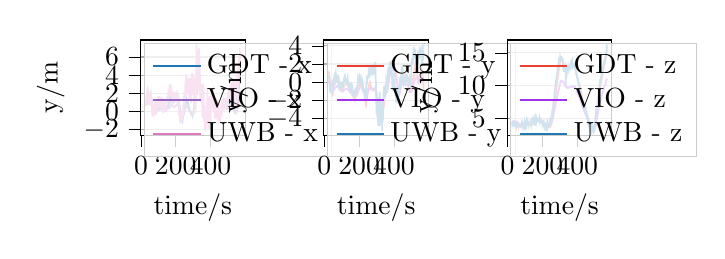
\begin{tikzpicture}

\definecolor{color0}{rgb}{0.91796875,0.25,0.203125}
\definecolor{color1}{rgb}{0.6328125,0.203125,0.91796875}
\definecolor{color2}{rgb}{0.12156862745098,0.466666666666667,0.705882352941177}
\definecolor{color3}{rgb}{0.580392156862745,0.403921568627451,0.741176470588235}
\definecolor{color4}{rgb}{0.890196078431372,0.466666666666667,0.76078431372549}
\definecolor{color5}{rgb}{0.854901960784314,0.647058823529412,0.125490196078431}
\definecolor{color6}{rgb}{0.980392156862745,0.501960784313725,0.447058823529412}
\definecolor{color7}{rgb}{0.627450980392157,0.32156862745098,0.176470588235294}

\begin{groupplot}[group style={group size=3 by 1}]
\nextgroupplot[
height=\figureheight,
width=\figurewidth,
legend cell align={left},
legend style={
  fill opacity=0.8,
  draw opacity=1,
  text opacity=1,
  at={(0.03,0.97)},
  anchor=north west,
  draw=white!80!black
},
tick align=outside,
tick pos=left,
x grid style={white!69.0196078431373!black},
xlabel={time/s},
xmin=-2.30530276513826, xmax=598.411358067903,
xtick style={color=black},
y grid style={white!69.0196078431373!black},
ylabel={y/m},
ymajorgrids,
ymin=-2.617, ymax=7.877,
ytick style={color=black}
]
\addplot [semithick, color2]
table {%
25 0.994737
25.6212810640532 0.998026
26.2425621281064 0.97138
26.8638431921596 0.973112
27.4851242562128 0.985128
28.106405320266 0.939383
28.7276863843192 0.953107
29.3489674483724 0.998548
29.9702485124256 0.979443
30.5915295764788 0.99938
31.212810640532 0.986651
31.8340917045852 1.069337
32.4553727686384 1.06078
33.0766538326916 1.077462
33.6979348967448 1.071065
34.319215960798 1.104277
34.9404970248512 1.179799
35.5617780889044 1.14207
36.1830591529576 1.145951
36.8043402170109 1.207792
37.4256212810641 1.218386
38.0469023451173 1.225895
38.6681834091705 1.24156
39.2894644732237 1.320253
39.9107455372769 1.35708
40.5320266013301 1.366109
41.1533076653833 1.371835
41.7745887294365 1.441461
42.3958697934897 1.405066
43.0171508575429 1.459378
43.6384319215961 1.589596
44.2597129856493 1.52353
44.8809940497025 1.635297
45.5022751137557 1.648012
46.1235561778089 1.737152
46.7448372418621 1.701654
47.3661183059153 1.739027
47.9873993699685 1.783488
48.6086804340217 1.839979
49.2299614980749 1.831476
49.8512425621281 1.89475
50.4725236261813 1.890742
51.0938046902345 1.85398
51.7150857542877 1.898961
52.3363668183409 1.867077
52.9576478823941 1.903204
53.5789289464473 1.870046
54.2002100105005 1.858369
54.8214910745537 1.905027
55.4427721386069 1.858811
56.0640532026601 1.804266
56.6853342667133 1.881858
57.3066153307665 1.730339
57.9278963948197 1.779049
58.5491774588729 1.699859
59.1704585229261 1.634726
59.7917395869794 1.583133
60.4130206510326 1.545948
61.0343017150858 1.488988
61.655582779139 1.447707
62.2768638431922 1.346701
62.8981449072454 1.321952
63.5194259712986 1.214165
64.1407070353518 1.179474
64.761988099405 1.079425
65.3832691634582 1.021266
66.0045502275114 0.940201
66.6258312915646 0.86749
67.2471123556178 0.743834
67.868393419671 0.678855
68.4896744837242 0.573933
69.1109555477774 0.475992
69.7322366118306 0.398611
70.3535176758838 0.331463
70.974798739937 0.265653
71.5960798039902 0.208428
72.2173608680434 0.151418
72.8386419320966 0.100698
73.4599229961498 0.050935
74.081204060203 0.006855
74.7024851242562 -0.006422
75.3237661883094 -0.029941
75.9450472523626 -0.055349
76.5663283164158 -0.072961
77.187609380469 -0.09934
77.8088904445222 -0.121137
78.4301715085754 -0.139172
79.0514525726286 -0.128364
79.6727336366818 -0.121963
80.294014700735 -0.128934
80.9152957647883 -0.15593
81.5365768288414 -0.161325
82.1578578928946 -0.175178
82.7791389569479 -0.161505
83.4004200210011 -0.157901
84.0217010850543 -0.151283
84.6429821491075 -0.161735
85.2642632131607 -0.150046
85.8855442772139 -0.136372
86.5068253412671 -0.106003
87.1281064053203 -0.08728
87.7493874693735 -0.025676
88.3706685334267 0.013777
88.9919495974799 0.042941
89.6132306615331 0.059884
90.2345117255863 0.084564
90.8557927896395 0.104568
91.4770738536927 0.132431
92.0983549177459 0.165201
92.7196359817991 0.176266
93.3409170458523 0.200914
93.9621981099055 0.212068
94.5834791739587 0.225688
95.2047602380119 0.233662
95.8260413020651 0.246702
96.4473223661183 0.255548
97.0686034301715 0.260814
97.6898844942247 0.247842
98.3111655582779 0.306455
98.9324466223311 0.275749
99.5537276863843 0.286878
100.175008750438 0.302095
100.796289814491 0.283683
101.417570878544 0.331735
102.038851942597 0.316653
102.66013300665 0.333917
103.281414070704 0.321046
103.902695134757 0.343015
104.52397619881 0.335846
105.145257262863 0.348922
105.766538326916 0.388795
106.38781939097 0.416848
107.009100455023 0.417746
107.630381519076 0.423614
108.251662583129 0.43281
108.872943647182 0.427392
109.494224711236 0.439371
110.115505775289 0.434597
110.736786839342 0.40489
111.358067903395 0.408774
111.979348967448 0.415771
112.600630031502 0.430542
113.221911095555 0.452641
113.843192159608 0.444958
114.464473223661 0.44228
115.085754287714 0.454894
115.707035351768 0.463503
116.328316415821 0.452484
116.949597479874 0.464339
117.570878543927 0.417793
118.19215960798 0.429406
118.813440672034 0.458333
119.434721736087 0.443736
120.05600280014 0.451694
120.677283864193 0.416266
121.298564928246 0.42433
121.9198459923 0.39067
122.541127056353 0.410114
123.162408120406 0.383446
123.783689184459 0.403952
124.404970248512 0.374077
125.026251312566 0.358935
125.647532376619 0.384167
126.268813440672 0.378286
126.890094504725 0.386069
127.511375568778 0.359722
128.132656632832 0.347831
128.753937696885 0.329688
129.375218760938 0.320412
129.996499824991 0.298259
130.617780889044 0.287524
131.239061953098 0.306839
131.860343017151 0.268423
132.481624081204 0.266342
133.102905145257 0.237009
133.72418620931 0.234785
134.345467273364 0.219194
134.966748337417 0.209641
135.58802940147 0.196333
136.209310465523 0.174627
136.830591529577 0.168033
137.45187259363 0.144428
138.073153657683 0.125379
138.694434721736 0.114407
139.315715785789 0.102414
139.936996849843 0.110715
140.558277913896 0.095648
141.179558977949 0.087645
141.800840042002 0.084951
142.422121106055 0.085608
143.043402170109 0.123042
143.664683234162 0.143736
144.285964298215 0.204338
144.907245362268 0.222794
145.528526426321 0.238398
146.149807490375 0.262778
146.771088554428 0.325787
147.392369618481 0.349629
148.013650682534 0.419383
148.634931746587 0.474522
149.256212810641 0.521488
149.877493874694 0.545526
150.498774938747 0.632728
151.1200560028 0.665645
151.741337066853 0.727632
152.362618130907 0.750064
152.98389919496 0.819683
153.605180259013 0.803746
154.226461323066 0.898666
154.847742387119 0.890705
155.469023451173 0.960188
156.090304515226 0.939688
156.711585579279 0.87963
157.332866643332 0.966768
157.954147707385 0.927128
158.575428771439 0.905796
159.196709835492 0.939062
159.817990899545 0.929965
160.439271963598 0.978125
161.060553027651 0.930258
161.681834091705 1.066851
162.303115155758 1.020459
162.924396219811 1.021286
163.545677283864 1.060694
164.166958347917 1.035419
164.788239411971 1.138803
165.409520476024 1.137856
166.030801540077 1.146264
166.65208260413 1.270515
167.273363668183 1.221112
167.894644732237 1.284518
168.51592579629 1.285095
169.137206860343 1.343149
169.758487924396 1.335057
170.379768988449 1.341098
171.001050052503 1.425354
171.622331116556 1.381899
172.243612180609 1.422262
172.864893244662 1.503061
173.486174308715 1.476487
174.107455372769 1.596921
174.728736436822 1.519635
175.350017500875 1.672552
175.971298564928 1.655537
176.592579628981 1.687864
177.213860693035 1.7052
177.835141757088 1.742722
178.456422821141 1.761743
179.077703885194 1.707158
179.698984949247 1.74074
180.320266013301 1.681402
180.941547077354 1.741965
181.562828141407 1.624541
182.18410920546 1.5522
182.805390269513 1.57609
183.426671333567 1.570578
184.04795239762 1.460228
184.669233461673 1.470094
185.290514525726 1.366847
185.91179558978 1.31422
186.533076653833 1.32172
187.154357717886 1.307063
187.775638781939 1.254953
188.396919845992 1.248769
189.018200910046 1.217766
189.639481974099 1.203125
190.260763038152 1.174537
190.882044102205 1.250206
191.503325166258 1.225722
192.124606230312 1.243644
192.745887294365 1.274291
193.367168358418 1.312183
193.988449422471 1.266958
194.609730486524 1.305944
195.231011550578 1.348278
195.852292614631 1.349525
196.473573678684 1.411316
197.094854742737 1.4143
197.71613580679 1.429254
198.337416870844 1.43219
198.958697934897 1.505008
199.57997899895 1.563655
200.201260063003 1.538844
200.822541127056 1.614945
201.44382219111 1.556184
202.065103255163 1.630873
202.686384319216 1.661641
203.307665383269 1.661282
203.928946447322 1.728823
204.550227511376 1.612603
205.171508575429 1.700703
205.792789639482 1.659419
206.414070703535 1.696657
207.035351767588 1.64695
207.656632831642 1.642365
208.277913895695 1.67067
208.899194959748 1.566
209.520476023801 1.617798
210.141757087854 1.553367
210.763038151908 1.544909
211.384319215961 1.547833
212.005600280014 1.459657
212.626881344067 1.534861
213.24816240812 1.403
213.869443472174 1.411342
214.490724536227 1.372932
215.11200560028 1.274222
215.733286664333 1.272542
216.354567728386 1.190933
216.97584879244 1.126438
217.597129856493 1.085471
218.218410920546 1.026984
218.839691984599 0.96497
219.460973048652 0.899625
220.082254112706 0.822566
220.703535176759 0.761851
221.324816240812 0.706389
221.946097304865 0.635443
222.567378368918 0.553477
223.188659432972 0.476249
223.809940497025 0.376378
224.431221561078 0.28565
225.052502625131 0.211043
225.673783689184 0.136745
226.295064753238 0.052995
226.916345817291 -0.031219
227.537626881344 -0.101429
228.158907945397 -0.165
228.78018900945 -0.240477
229.401470073504 -0.31046
230.022751137557 -0.354327
230.64403220161 -0.402496
231.265313265663 -0.47335
231.886594329717 -0.445361
232.50787539377 -0.484362
233.129156457823 -0.553018
233.750437521876 -0.561947
234.371718585929 -0.601191
234.992999649983 -0.624203
235.614280714036 -0.718071
236.235561778089 -0.642173
236.856842842142 -0.613787
237.478123906195 -0.697736
238.099404970249 -0.62064
238.720686034302 -0.64389
239.341967098355 -0.727661
239.963248162408 -0.6358
240.584529226461 -0.6956
241.205810290515 -0.579897
241.827091354568 -0.589538
242.448372418621 -0.538494
243.069653482674 -0.54989
243.690934546727 -0.471797
244.312215610781 -0.395889
244.933496674834 -0.4095
245.554777738887 -0.412328
246.17605880294 -0.248231
246.797339866993 -0.241322
247.418620931047 -0.181072
248.0399019951 -0.139273
248.661183059153 -0.067955
249.282464123206 0.018473
249.903745187259 0.058132
250.525026251313 0.148173
251.146307315366 0.187894
251.767588379419 0.234832
252.388869443472 0.326105
253.010150507525 0.407351
253.631431571579 0.480304
254.252712635632 0.534649
254.873993699685 0.584596
255.495274763738 0.745082
256.116555827791 0.799124
256.737836891845 0.833107
257.359117955898 0.946546
257.980399019951 1.015672
258.601680084004 1.099
259.222961148057 1.138481
259.844242212111 1.234033
260.465523276164 1.222768
261.086804340217 1.339846
261.70808540427 1.280044
262.329366468323 1.331784
262.950647532377 1.316821
263.57192859643 1.252136
264.193209660483 1.322821
264.814490724536 1.290522
265.435771788589 1.240009
266.057052852643 1.247198
266.678333916696 1.17118
267.299614980749 1.160731
267.920896044802 1.107793
268.542177108855 1.081478
269.163458172909 1.002846
269.784739236962 0.966022
270.406020301015 0.9345
271.027301365068 0.856196
271.648582429121 0.790274
272.269863493175 0.751177
272.891144557228 0.720206
273.512425621281 0.652218
274.133706685334 0.61503
274.754987749388 0.571149
275.376268813441 0.528953
275.997549877494 0.471185
276.618830941547 0.445346
277.2401120056 0.372857
277.861393069654 0.342766
278.482674133707 0.28115
279.10395519776 0.259855
279.725236261813 0.237206
280.346517325866 0.190252
280.967798389919 0.153657
281.589079453973 0.141833
282.210360518026 0.086635
282.831641582079 0.059915
283.452922646132 0.028495
284.074203710186 -0.010871
284.695484774239 -0.016183
285.316765838292 -0.058523
285.938046902345 -0.096451
286.559327966398 -0.138743
287.180609030452 -0.180068
287.801890094505 -0.220019
288.423171158558 -0.232373
289.044452222611 -0.290339
289.665733286664 -0.315623
290.287014350718 -0.338404
290.908295414771 -0.380969
291.529576478824 -0.404407
292.150857542877 -0.435876
292.77213860693 -0.435952
293.393419670984 -0.438733
294.014700735037 -0.443704
294.63598179909 -0.450964
295.257262863143 -0.419506
295.878543927196 -0.470123
296.49982499125 -0.41242
297.121106055303 -0.391388
297.742387119356 -0.338577
298.363668183409 -0.293442
298.984949247462 -0.282026
299.606230311516 -0.207886
300.227511375569 -0.145542
300.848792439622 -0.097179
301.470073503675 -0.070763
302.091354567728 0.022278
302.712635631782 0.096478
303.333916695835 0.204963
303.955197759888 0.367647
304.576478823941 0.353947
305.197759887994 0.536857
305.819040952048 0.531773
306.440322016101 0.750592
307.061603080154 0.830435
307.682884144207 0.996179
308.30416520826 1.135941
308.925446272314 1.250318
309.546727336367 1.378833
310.16800840042 1.594304
310.789289464473 1.6235
311.410570528526 1.897
312.03185159258 1.991577
312.653132656633 2.163882
313.274413720686 2.362833
313.895694784739 2.5677
314.516975848792 2.65868
315.138256912846 2.887308
315.759537976899 2.8579
316.380819040952 3.078
317.002100105005 3.036572
317.623381169058 3.177222
318.244662233112 3.24175
318.865943297165 3.1972
319.487224361218 3.3125
320.108505425271 3.329479
320.729786489325 3.46575
321.351067553378 3.47545
321.972348617431 3.497
322.593629681484 3.618629
323.214910745537 3.727
323.836191809591 3.871257
324.457472873644 3.904
325.078753937697 3.8905
325.70003500175 4.130766
326.321316065803 4.372
326.942597129856 4.408381
327.56387819391 4.733111
328.185159257963 4.764222
328.806440322016 4.864667
329.427721386069 4.887445
330.049002450123 4.9845
330.670283514176 4.868846
331.291564578229 4.937091
331.912845642282 4.8887
332.534126706335 4.9352
333.155407770389 4.698822
333.776688834442 4.434
334.397969898495 4.462722
335.019250962548 4.421667
335.640532026601 4.284334
336.261813090655 3.95225
336.883094154708 3.937333
337.504375218761 3.637
338.125656282814 3.5894
338.746937346867 3.432273
339.368218410921 3.370885
339.989499474974 3.217636
340.610780539027 3.123531
341.23206160308 2.992417
341.853342667133 2.922121
342.474623731187 2.593
343.09590479524 2.831966
343.717185859293 2.836917
344.338466923346 2.777737
344.959747987399 2.69075
345.581029051453 2.699289
346.202310115506 2.572167
346.823591179559 2.565817
347.444872243612 2.490059
348.066153307665 2.475796
348.687434371719 2.4048
349.308715435772 2.373929
349.929996499825 2.395105
350.551277563878 2.338353
351.172558627931 2.283362
351.793839691985 2.213
352.415120756038 2.132679
353.036401820091 2.010423
353.657682884144 1.9746
354.278963948197 1.76425
354.900245012251 1.703611
355.521526076304 1.545417
356.142807140357 1.426434
356.76408820441 1.267759
357.385369268463 1.059143
358.006650332517 0.94363
358.62793139657 0.822683
359.249212460623 0.654141
359.870493524676 0.487242
360.491774588729 0.345051
361.113055652783 0.237667
361.734336716836 0.112256
362.355617780889 0.007037
362.976898844942 -0.124936
363.598179908995 -0.223929
364.219460973049 -0.302831
364.840742037102 -0.37499
365.462023101155 -0.456566
366.083304165208 -0.513269
366.704585229262 -0.578468
367.325866293315 -0.591309
367.947147357368 -0.628412
368.568428421421 -0.713153
369.189709485474 -0.7557
369.810990549528 -0.811805
370.432271613581 -0.821068
371.053552677634 -0.847441
371.674833741687 -0.863
372.29611480574 -0.932415
372.917395869793 -0.904183
373.538676933847 -0.917717
374.1599579979 -0.929226
374.781239061953 -0.952283
375.402520126006 -0.931652
376.02380119006 -0.948489
376.645082254113 -0.926074
377.266363318166 -0.913885
377.887644382219 -0.894212
378.508925446272 -0.862104
379.130206510326 -0.830163
379.751487574379 -0.83307
380.372768638432 -0.750371
380.994049702485 -0.788515
381.615330766538 -0.723921
382.236611830592 -0.6344
382.857892894645 -0.657152
383.479173958698 -0.627563
384.100455022751 -0.543081
384.721736086804 -0.555703
385.343017150858 -0.475553
385.964298214911 -0.431184
386.585579278964 -0.395447
387.206860343017 -0.327974
387.82814140707 -0.310857
388.449422471124 -0.218311
389.070703535177 -0.1775
389.69198459923 -0.214909
390.313265663283 -0.091278
390.934546727336 -0.084583
391.55582779139 -0.085114
392.177108855443 0.056839
392.798389919496 0.040333
393.419670983549 0.110842
394.040952047602 0.174028
394.662233111656 0.255833
395.283514175709 0.295881
395.904795239762 0.361725
396.526076303815 0.485
397.147357367868 0.493356
397.768638431922 0.588921
398.389919495975 0.600694
399.011200560028 0.679611
399.632481624081 0.739906
400.253762688134 0.811611
400.875043752188 0.901513
401.496324816241 0.922636
402.117605880294 1.007452
402.738886944347 1.071674
403.3601680084 1.182837
403.981449072454 1.262468
404.602730136507 1.307317
405.22401120056 1.401286
405.845292264613 1.548681
406.466573328666 1.536278
407.08785439272 1.645551
407.709135456773 1.774056
408.330416520826 1.77075
408.951697584879 1.834384
409.572978648932 1.947237
410.194259712986 1.940452
410.815540777039 1.9645
411.436821841092 1.952186
412.058102905145 1.949413
412.679383969199 1.934095
413.300665033252 1.989414
413.921946097305 1.908878
414.543227161358 1.892981
415.164508225411 1.985367
415.785789289465 1.829098
416.407070353518 1.799071
417.028351417571 1.794409
417.649632481624 1.733839
418.270913545677 1.604828
418.89219460973 1.594
419.513475673784 1.512536
420.134756737837 1.351125
420.75603780189 1.27337
421.377318865943 1.207375
421.998599929997 1.079118
422.61988099405 0.973557
423.241162058103 0.808642
423.862443122156 0.720444
424.483724186209 0.611206
425.105005250263 0.531311
425.726286314316 0.447731
426.347567378369 0.389375
426.968848442422 0.313674
427.590129506475 0.245442
428.211410570529 0.232487
428.832691634582 0.18943
429.453972698635 0.140793
430.075253762688 0.102429
430.696534826741 0.089378
431.317815890795 0.088406
431.939096954848 0.066827
432.560378018901 0.084536
433.181659082954 0.093545
433.802940147007 0.122689
434.424221211061 0.167509
435.045502275114 0.210963
435.666783339167 0.262548
436.28806440322 0.297607
436.909345467273 0.312398
437.530626531327 0.316915
438.15190759538 0.354934
438.773188659433 0.358508
439.394469723486 0.401555
440.015750787539 0.381161
440.637031851593 0.377287
441.258312915646 0.389835
441.879593979699 0.41906
442.500875043752 0.431455
443.122156107805 0.415995
443.743437171859 0.391846
444.364718235912 0.368149
444.985999299965 0.330258
445.607280364018 0.303951
446.228561428071 0.251384
446.849842492125 0.217197
447.471123556178 0.161617
448.092404620231 0.117067
448.713685684284 0.07828
449.334966748337 0.016246
449.956247812391 -0.060517
450.577528876444 -0.099517
451.198809940497 -0.138009
451.82009100455 -0.176731
452.441372068603 -0.232369
453.062653132657 -0.243482
453.68393419671 -0.288259
454.305215260763 -0.276048
454.926496324816 -0.277967
455.547777388869 -0.280882
456.169058452923 -0.329869
456.790339516976 -0.317186
457.411620581029 -0.291938
458.032901645082 -0.260892
458.654182709136 -0.232797
459.275463773189 -0.20992
459.896744837242 -0.17535
460.518025901295 -0.124665
461.139306965348 -0.098157
461.760588029402 -0.061409
462.381869093455 -0.008514
463.003150157508 0.023262
463.624431221561 0.06316
464.245712285614 0.104959
464.866993349667 0.156063
465.488274413721 0.208202
466.109555477774 0.262886
466.730836541827 0.311997
467.35211760588 0.377412
467.973398669934 0.448504
468.594679733987 0.487076
469.21596079804 0.577377
469.837241862093 0.633589
470.458522926146 0.672453
471.0798039902 0.764571
471.701085054253 0.809604
472.322366118306 0.881665
472.943647182359 0.893523
473.564928246412 0.98208
474.186209310466 0.958939
474.807490374519 0.988442
475.428771438572 0.995364
476.050052502625 1.025223
476.671333566678 0.97598
477.292614630732 1.022868
477.913895694785 0.947304
478.535176758838 0.968695
479.156457822891 0.972256
479.777738886944 0.883013
480.399019950998 0.888927
481.020301015051 0.908004
481.641582079104 0.835
482.262863143157 0.790751
482.88414420721 0.749932
483.505425271264 0.729764
484.126706335317 0.695349
484.74798739937 0.648863
485.369268463423 0.613246
485.990549527476 0.593579
486.61183059153 0.572399
487.233111655583 0.581058
487.854392719636 0.532495
488.475673783689 0.496848
489.096954847742 0.480019
489.718235911796 0.487288
490.339516975849 0.464655
490.960798039902 0.463826
491.582079103955 0.447174
492.203360168008 0.483686
492.824641232062 0.483618
493.445922296115 0.480055
494.067203360168 0.503136
494.688484424221 0.498132
495.309765488274 0.523208
495.931046552328 0.585826
496.552327616381 0.654379
497.173608680434 0.665272
497.794889744487 0.726705
498.41617080854 0.747368
499.037451872594 0.812863
499.658732936647 0.888083
500.2800140007 0.907843
500.901295064753 0.919049
501.522576128806 0.944198
502.14385719286 1.029409
502.765138256913 0.976651
503.386419320966 0.998033
504.007700385019 0.999855
504.628981449073 1.012234
505.250262513126 1.002508
505.871543577179 1.030541
506.492824641232 1.066337
507.114105705285 1.028609
507.735386769339 1.070125
508.356667833392 1.117184
508.977948897445 1.054609
509.599229961498 1.108379
510.220511025551 1.177261
510.841792089604 1.144434
511.463073153658 1.211701
512.084354217711 1.253545
512.705635281764 1.225103
513.326916345817 1.275936
513.948197409871 1.262675
514.569478473924 1.348459
515.190759537977 1.318961
515.81204060203 1.373273
516.433321666083 1.399194
517.054602730137 1.465043
517.67588379419 1.440195
518.297164858243 1.567972
518.918445922296 1.498714
519.539726986349 1.5428
520.161008050403 1.565604
520.782289114456 1.496764
521.403570178509 1.566654
522.024851242562 1.44687
522.646132306615 1.504791
523.267413370669 1.376389
523.888694434722 1.435457
524.509975498775 1.294357
525.131256562828 1.306449
525.752537626881 1.218909
526.373818690935 1.134316
526.995099754988 1.094866
527.616380819041 1.001429
528.237661883094 0.930962
528.858942947147 0.812064
529.480224011201 0.728612
530.101505075254 0.632878
530.722786139307 0.580736
531.34406720336 0.479151
531.965348267413 0.408772
532.586629331467 0.344758
533.20791039552 0.288053
533.829191459573 0.207026
534.450472523626 0.192938
535.071753587679 0.14384
535.693034651733 0.097608
536.314315715786 0.048329
536.935596779839 0.001455
537.556877843892 -0.015906
538.178158907945 -0.040641
538.799439971999 -0.058933
539.420721036052 -0.067239
540.042002100105 -0.07195
540.663283164158 -0.070098
541.284564228211 -0.089257
541.905845292265 -0.067768
542.527126356318 -0.061174
543.148407420371 -0.040177
543.769688484424 -0.02239
544.390969548477 -0.000313
545.012250612531 0.045134
545.633531676584 0.076519
546.254812740637 0.109656
546.87609380469 0.143276
547.497374868743 0.19945
548.118655932797 0.256135
548.73993699685 0.296958
549.361218060903 0.344876
549.982499124956 0.439244
550.60378018901 0.515412
551.225061253063 0.549846
551.846342317116 0.616028
552.467623381169 0.716196
553.088904445222 0.778698
553.710185509276 0.880244
554.331466573329 0.86322
554.952747637382 0.9618
555.574028701435 1.102
556.195309765488 1.107486
556.816590829541 1.271462
557.437871893595 1.390857
558.059152957648 1.582951
558.680434021701 1.760773
559.301715085754 1.865821
559.922996149808 2.045923
560.544277213861 2.312739
561.165558277914 2.390239
561.786839341967 2.546314
562.40812040602 2.707862
563.029401470074 2.859527
563.650682534127 3.060934
564.27196359818 3.023303
564.893244662233 3.242061
565.514525726286 3.517369
566.13580679034 3.493967
566.757087854393 3.556454
567.378368918446 3.719909
567.999649982499 3.924605
568.620931046552 4.080143
569.242212110606 4.106834
569.863493174659 4.263451
570.484774238712 4.087
571.106055302765 4.351069
};
\addlegendentry{GDT - x}
\addplot [semithick, color3]
table {%
25.0219490781387 0.801387733221
25.5223880597015 0.801826423407
26.0228270412643 0.804013258219
26.523266022827 0.784632360935
27.0237050043898 0.783451145887
27.5241439859526 0.779182171822
28.0245829675154 0.773093080521
28.5250219490781 0.766327029467
29.0254609306409 0.742100811005
29.5258999122037 0.73946557045
30.0263388937665 0.726899510622
30.5267778753292 0.720703548193
31.027216856892 0.717529958487
31.5276558384548 0.717361098528
32.0280948200176 0.728716379404
32.5285338015803 0.738685792685
33.0289727831431 0.743106281757
33.5294117647059 0.742942368984
34.0298507462687 0.741564846039
34.5302897278314 0.744070625305
35.0307287093942 0.750786310434
35.531167690957 0.754612869024
36.0316066725198 0.764468467236
36.5320456540825 0.774770534039
37.0324846356453 0.791829144955
37.5329236172081 0.800479507446
38.0333625987709 0.828493154049
38.5338015803336 0.851081109047
39.0342405618964 0.867623335123
39.5346795434592 0.875924727321
40.0351185250219 0.887741467357
40.5355575065847 0.916617146134
41.0359964881475 0.924934929609
41.5364354697103 0.943141466379
42.036874451273 0.957936128974
42.5373134328358 0.969433760643
43.0377524143986 0.996792717278
43.5381913959614 1.0056875407696
44.0386303775241 1.0241574779153
44.5390693590869 1.0377258978784
45.0395083406497 1.0483204334974
45.5399473222125 1.0658205546439
46.0403863037752 1.084605146572
46.540825285338 1.10563320284709
47.0412642669008 1.1119455223903
47.5417032484636 1.1145899988711
48.0421422300263 1.1439148806036
48.5425812115891 1.1668411925435
49.0430201931519 1.1772105306387
49.5434591747147 1.1720500126481
50.0438981562774 1.1813301354647
50.5443371378402 1.1868685618043
51.044776119403 1.1825160816312
51.5452151009658 1.1685257911682
52.0456540825285 1.1544689334929
52.5460930640913 1.1478995367885
53.0465320456541 1.1344288907945
53.5469710272169 1.1296995267272
54.0474100087796 1.1131265399978
54.5478489903424 1.10793181639165
55.0482879719052 1.10528988428414
55.5487269534679 1.09745331495069
56.0491659350307 1.09220216553658
56.5496049165935 1.0850437156856
57.0500438981563 1.0802409913391
57.550482879719 1.0662088565528
58.0509218612818 1.0464804381132
58.5513608428446 1.0429060332477
59.0517998244074 1.0325636997819
59.5522388059701 1.0118000641465
60.0526777875329 1.0021504446864
60.5531167690957 0.974100297689
61.0535557506585 0.950243315101
61.5539947322212 0.932171306014
62.054433713784 0.909566408396
62.5548726953468 0.886336541176
63.0553116769096 0.863342604041
63.5557506584723 0.829607075453
64.0561896400351 0.803404515982
64.5566286215979 0.775676971674
65.0570676031607 0.744665688276
65.5575065847234 0.707566595078
66.0579455662862 0.670498436689
66.558384547849 0.63598600626
67.0588235294118 0.631701117754
67.5592625109745 0.601554578543
68.0597014925373 0.560273504257
68.5601404741001 0.543686664104
69.0605794556629 0.477654314041
69.5610184372256 0.457204496861
70.0614574187884 0.409691131115
70.5618964003512 0.378056919575
71.062335381914 0.360915875435
71.5627743634767 0.330543911457
72.0632133450395 0.295072770119
72.5636523266023 0.255219733715
73.064091308165 0.238727605343
73.5645302897278 0.205223059654
74.0649692712906 0.154290652275
74.5654082528534 0.141603326797
75.0658472344162 0.106074011326
75.5662862159789 0.08601591587
76.0667251975417 0.0652078151700002
76.5671641791045 0.0389156103100001
77.0676031606672 0.01651856899
77.56804214223 0.00754282475000001
78.0684811237928 -0.01442697048
78.5689201053556 -0.0229268312499999
79.0693590869183 -0.0454979181299999
79.5697980684811 -0.03614475727
80.0702370500439 -0.0377077102699999
80.5706760316067 -0.05295445919
81.0711150131694 -0.0553542614
81.5715539947322 -0.07092859745
82.071992976295 -0.07223846912
82.5724319578578 -0.0812291145299999
83.0728709394205 -0.0864471435499998
83.5733099209833 -0.09190061092
84.0737489025461 -0.0876982450499999
84.5741878841089 -0.0890060901599998
85.0746268656716 -0.0875933408699998
85.5750658472344 -0.0943557262399999
86.0755048287972 -0.09256556034
86.57594381036 -0.0832823753399998
87.0763827919227 -0.0844789981799998
87.5768217734855 -0.0719057559999998
88.0772607550483 -0.0525399684899999
88.5776997366111 -0.0440412998199999
89.0781387181738 -0.0384103298199998
89.5785776997366 -0.0223515272099999
90.0790166812994 -0.0139227151899999
90.5794556628622 0.00696239471000015
91.0798946444249 0.024472332
91.5803336259877 0.0317972660100001
92.0807726075505 0.0465924501400001
92.5812115891133 0.0568624496500001
93.081650570676 0.0629946947100002
93.5820895522388 0.0747323989900002
94.0825285338016 0.0814069271100002
94.5829675153643 0.0915726184800001
95.0834064969271 0.100509142876
95.5838454784899 0.0999730587000001
96.0842844600527 0.109467601776
96.5847234416155 0.121154522896
97.0851624231782 0.124456262589
97.585601404741 0.13570574522
98.0860403863038 0.140887594223
98.5864793678665 0.151072776318
99.0869183494293 0.150805211067
99.5873573309921 0.156860268116
100.087796312555 0.15884885788
100.588235294118 0.159741735458
101.08867427568 0.160258507729
101.589113257243 0.161281561852
102.089552238806 0.164746975899
102.589991220369 0.169772541523
103.090430201932 0.175890243053
103.590869183494 0.177179193497
104.091308165057 0.186538016796
104.59174714662 0.192692196369
105.092186128183 0.203784561157
105.592625109745 0.207042789459
106.093064091308 0.212599790096
106.593503072871 0.224634087086
107.093942054434 0.229049897194
107.594381035996 0.228857195377
108.094820017559 0.230819618702
108.595258999122 0.231384372711
109.095697980685 0.228707945347
109.596136962248 0.227481341362
110.09657594381 0.228795206547
110.597014925373 0.228626286983
111.097453906936 0.224972343445
111.597892888499 0.221998369694
112.098331870061 0.218744432926
112.598770851624 0.219939506054
113.099209833187 0.218119180202
113.59964881475 0.214174962044
114.100087796313 0.215163862705
114.600526777875 0.209385550022
115.100965759438 0.204741454124
115.601404741001 0.206225848198
116.101843722564 0.205763852596
116.602282704126 0.21312353611
117.102721685689 0.214822626114
117.603160667252 0.217718875408
118.103599648815 0.219205951691
118.604038630378 0.217186427116
119.10447761194 0.211507773399
119.604916593503 0.213953471184
120.105355575066 0.21544919014
120.605794556629 0.213510489464
121.106233538191 0.217400765419
121.606672519754 0.225611484051
122.107111501317 0.229912376404
122.60755048288 0.225819802284
123.107989464442 0.225418245792
123.608428446005 0.218111670017
124.108867427568 0.217427527905
124.609306409131 0.216382956505
125.109745390694 0.211888825893
125.610184372256 0.209529793262
126.110623353819 0.207519209385
126.611062335382 0.20470187664
127.111501316945 0.210196769238
127.611940298507 0.210822796822
128.11237928007 0.223569011688
128.612818261633 0.228226161003
129.113257243196 0.232453203201
129.613696224759 0.23540750742
130.114135206321 0.235988533497
130.614574187884 0.230597174168
131.115013169447 0.221760845184
131.61545215101 0.214899992943
132.115891132572 0.210636651516
132.616330114135 0.206644809246
133.116769095698 0.197541034222
133.617208077261 0.193354225159
134.117647058824 0.17753098011
134.618086040386 0.172931468487
135.118525021949 0.16804984808
135.618964003512 0.164884662628
136.119402985075 0.161482548714
136.619841966637 0.156008815765
137.1202809482 0.139979398251
137.620719929763 0.137771165371
138.121158911326 0.13642141819
138.621597892889 0.126700913906
139.122036874451 0.121400272846
139.622475856014 0.116334474087
140.122914837577 0.102179920673
140.62335381914 0.100543415546
141.123792800702 0.0974023103700001
141.624231782265 0.09387681484
142.124670763828 0.09709033966
142.625109745391 0.106904482841
143.125548726953 0.101591145992
143.625987708516 0.110125815868
144.126426690079 0.118925428391
144.626865671642 0.125842547417
145.127304653205 0.138866579533
145.627743634767 0.160368299484
146.12818261633 0.176335847378
146.628621597893 0.181545233727
147.129060579456 0.191709315777
147.629499561018 0.201980030537
148.129938542581 0.222519850731
148.630377524144 0.231188750267
149.130816505707 0.245656824112
149.63125548727 0.266020810604
150.131694468832 0.274459695816
150.632133450395 0.294101929665
151.132572431958 0.313190317154
151.633011413521 0.322492098808
152.133450395083 0.32741985321
152.633889376646 0.34536293745
153.134328358209 0.348210608959
153.634767339772 0.355447506905
154.135206321334 0.35571346283
154.635645302897 0.35387853384
155.13608428446 0.350726282597
155.636523266023 0.34979865551
156.136962247586 0.348260319233
156.637401229148 0.345722770691
157.137840210711 0.313086307049
157.638279192274 0.302819645405
158.138718173837 0.300071692467
158.639157155399 0.296788370609
159.139596136962 0.301646864414
159.640035118525 0.302269971371
160.140474100088 0.314284539223
160.640913081651 0.326173758507
161.141352063213 0.340120053291
161.641791044776 0.344300186634
162.142230026339 0.354526495934
162.642669007902 0.37195507288
163.143107989464 0.374468839169
163.643546971027 0.387780344486
164.14398595259 0.403752720356
164.644424934153 0.413517212868
165.144863915716 0.428224599361
165.645302897278 0.441674983501
166.145741878841 0.450423395634
166.646180860404 0.463651096821
167.146619841967 0.471416985989
167.647058823529 0.490385329723
168.147497805092 0.501141405106
168.647936786655 0.515124773979
169.148375768218 0.523187255859
169.64881474978 0.537285542488
170.149253731343 0.549283182621
170.649692712906 0.558599925041
171.150131694469 0.565612649918
171.650570676032 0.578501975536
172.151009657594 0.596313989162
172.651448639157 0.608624523878
173.15188762072 0.61649326086
173.652326602283 0.630815601349
174.152765583845 0.651588743925
174.653204565408 0.672190523148
175.153643546971 0.681285178661
175.654082528534 0.699547237158
176.154521510097 0.711534416676
176.654960491659 0.718279218674
177.155399473222 0.712186163664
177.655838454785 0.706952697039
178.156277436348 0.704052692652
178.65671641791 0.695212340355
179.157155399473 0.690556800365
179.657594381036 0.680258458853
180.158033362599 0.671711659431
180.658472344162 0.668652451038
181.158911325724 0.652376031876
181.659350307287 0.639059400558
182.15978928885 0.632829105854
182.660228270413 0.618036901951
183.160667251975 0.606329625845
183.661106233538 0.586988544464
184.161545215101 0.568125760555
184.661984196664 0.555314338207
185.162423178227 0.542057549953
185.662862159789 0.530479049683
186.163301141352 0.521820580959
186.663740122915 0.512446796894
187.164179104478 0.498603200912
187.66461808604 0.495022630692
188.165057067603 0.489390468597
188.665496049166 0.488845086098
189.165935030729 0.483707404137
189.666374012291 0.476846075058
190.166812993854 0.476942753792
190.667251975417 0.481119012833
191.16769095698 0.483880376816
191.668129938543 0.487600541115
192.168568920105 0.495701289177
192.669007901668 0.502724027634
193.169446883231 0.508864378929
193.669885864794 0.515318012238
194.170324846356 0.51773223877
194.670763827919 0.525957560539
195.171202809482 0.542251741886
195.671641791045 0.557023620605
196.172080772608 0.563132143021
196.67251975417 0.583761787415
197.172958735733 0.58545140028
197.673397717296 0.59920809269
198.173836698859 0.606115376949
198.674275680421 0.609160339832
199.174714661984 0.610032862425
199.675153643547 0.618107682467
200.17559262511 0.631884074211
200.676031606672 0.637014633417
201.176470588235 0.642905688286
201.676909569798 0.6485432446
202.177348551361 0.653564876318
202.677787532924 0.65529999733
203.178226514486 0.660464203358
203.678665496049 0.659628605843
204.179104477612 0.659311628342
204.679543459175 0.686855232716
205.179982440737 0.717186754942
205.6804214223 0.730071461201
206.180860403863 0.742701417208
206.681299385426 0.747408932447
207.181738366989 0.743343120813
207.682177348551 0.737211889029
208.182616330114 0.732375955582
208.683055311677 0.717504715919
209.18349429324 0.709709262848
209.683933274802 0.694374537468
210.184372256365 0.688865309954
210.684811237928 0.679376727343
211.185250219491 0.671092426777
211.685689201054 0.665002888441
212.186128182616 0.653823500872
212.686567164179 0.636296457052
213.187006145742 0.627989059687
213.687445127305 0.62230861783
214.187884108867 0.595198190212
214.68832309043 0.58682898283
215.188762071993 0.562296068668
215.689201053556 0.55003002882
216.189640035119 0.532101845741
216.690079016681 0.505467569828
217.190517998244 0.480033135414
217.690956979807 0.464923775196
218.19139596137 0.433476603031
218.691834942932 0.397020077705
219.192273924495 0.377564764023
219.692712906058 0.366648650169
220.193151887621 0.326482450962
220.693590869183 0.306853151321
221.194029850746 0.295409834385
221.694468832309 0.265234327316
222.194907813872 0.241566634178
222.695346795435 0.20068243742
223.195785776997 0.179746901989
223.69622475856 0.137730276585
224.196663740123 0.106676375866
224.697102721686 0.0638675451300001
225.197541703248 0.0424301385900001
225.697980684811 0.01810512543
226.198419666374 -0.02401247025
226.698858647937 -0.06755616665
227.1992976295 -0.0699970960599998
227.699736611062 -0.11558475494
228.200175592625 -0.12900772095
228.700614574188 -0.16100218296
229.201053555751 -0.1874519825
229.701492537313 -0.2036621809
230.201931518876 -0.21688988209
230.702370500439 -0.23484220505
231.202809482002 -0.24298491478
231.703248463565 -0.24845030308
232.203687445127 -0.25145699978
232.70412642669 -0.25746920109
233.204565408253 -0.26568272114
233.705004389816 -0.26854529381
234.205443371378 -0.27494790554
234.705882352941 -0.2827855587
235.206321334504 -0.29108610153
235.706760316067 -0.29431667328
236.207199297629 -0.30271067619
236.707638279192 -0.3127548933
237.208077260755 -0.32079985142
237.708516242318 -0.32132663727
238.208955223881 -0.32813265324
238.709394205443 -0.33213474751
239.209833187006 -0.31081440449
239.710272168569 -0.30698504448
240.210711150132 -0.30052056313
240.711150131694 -0.30099132061
241.211589113257 -0.3042391777
241.71202809482 -0.29024436474
242.212467076383 -0.27860846519
242.712906057946 -0.27682509422
243.213345039508 -0.25973858833
243.713784021071 -0.25206508636
244.214223002634 -0.24204161167
244.714661984197 -0.23027911186
245.215100965759 -0.20978989601
245.715539947322 -0.1865793705
246.215978928885 -0.1815798521
246.716417910448 -0.15881898403
247.216856892011 -0.12744882107
247.717295873573 -0.10964586735
248.217734855136 -0.10610654354
248.718173836699 -0.06419517994
249.218612818262 -0.04028668404
249.719051799824 -0.0283800601999999
250.219490781387 0.0062868356700001
250.71992976295 0.0516639709500002
251.220368744513 0.07225224972
251.720807726075 0.09259269238
252.221246707638 0.13164434433
252.721685689201 0.152605807781
253.222124670764 0.190002298355
253.722563652327 0.20812497139
254.223002633889 0.242873585224
254.723441615452 0.296476459503
255.223880597015 0.322525119781
255.724319578578 0.354605770111
256.22475856014 0.397493159771
256.725197541703 0.445394730568
257.225636523266 0.463979637623
257.726075504829 0.494187629223
258.226514486392 0.512084579468
258.726953467954 0.533138430119
259.227392449517 0.551324641705
259.72783143108 0.583451843262
260.228270412643 0.59731451273
260.728709394205 0.614057934284
261.229148375768 0.624490714073
261.729587357331 0.62675190568
262.230026338894 0.649589842558
262.730465320457 0.655752128363
263.230904302019 0.669181054831
263.731343283582 0.65382412672
264.231782265145 0.642185008526
264.732221246708 0.63866609931
265.23266022827 0.608926361799
265.733099209833 0.597673690319
266.233538191396 0.585556960106
266.733977172959 0.558982586861
267.234416154522 0.537140703201
267.734855136084 0.513289010525
268.235294117647 0.500374472141
268.73573309921 0.478226459026
269.236172080773 0.437545514107
269.736611062335 0.423470771313
270.237050043898 0.405166006088
270.737489025461 0.371566867828
271.237928007024 0.331038510799
271.738366988586 0.314364230633
272.238805970149 0.300178384781
272.739244951712 0.276113367081
273.239683933275 0.254279053211
273.740122914838 0.233262276649
274.2405618964 0.200300908089
274.741000877963 0.174510157108
275.241439859526 0.163795745373
275.741878841089 0.143364167213
276.242317822651 0.118350839615
276.742756804214 0.105729317665
277.243195785777 0.0966770410500002
277.74363476734 0.0839935302700001
278.244073748903 0.0754903316500002
278.744512730465 0.0464207887600001
279.244951712028 0.02928433418
279.745390693591 0.01986513138
280.245829675154 0.00713131428000002
280.746268656716 0.00551626682000017
281.246707638279 0.0064399004000002
281.747146619842 -0.00269427298999991
282.247585601405 -0.01216461658
282.748024582968 -0.0354334354399999
283.24846356453 -0.03799452782
283.748902546093 -0.0666274070699999
284.249341527656 -0.0767959594699998
284.749780509219 -0.10856416225
285.250219490781 -0.12433590889
285.750658472344 -0.15578272343
286.251097453907 -0.16488661766
286.75153643547 -0.19205155373
287.251975417032 -0.21822788715
287.752414398595 -0.22904469967
288.252853380158 -0.24644579887
288.753292361721 -0.28040924072
289.253731343284 -0.28952386379
289.754170324846 -0.30301465988
290.254609306409 -0.33449997902
290.755048287972 -0.35011711121
291.255487269535 -0.3613597393
291.755926251097 -0.3814208746
292.25636523266 -0.39167501926
292.756804214223 -0.39839019775
293.257243195786 -0.40640285015
293.757682177349 -0.4018787384
294.258121158911 -0.42063441277
294.758560140474 -0.42794897556
295.258999122037 -0.42476596832
295.7594381036 -0.41774597168
296.259877085162 -0.41421558857
296.760316066725 -0.39795114994
297.260755048288 -0.39195384979
297.761194029851 -0.37073876858
298.261633011413 -0.35351576805
298.762071992976 -0.34166374207
299.262510974539 -0.33086707592
299.762949956102 -0.30629792213
300.263388937665 -0.28592290878
300.763827919227 -0.27340509892
301.26426690079 -0.24799253941
301.764705882353 -0.20292737484
302.265144863916 -0.18461742401
302.765583845478 -0.13817324638
303.266022827041 -0.11296572685
303.766461808604 -0.0422317027999999
304.266900790167 0.00905141830000011
304.76733977173 0.0249423742300001
305.267778753292 0.0986261129400001
305.768217734855 0.134628093243
306.268656716418 0.191096997261
306.769095697981 0.226163721085
307.269534679543 0.325535094738
307.769973661106 0.394025838375
308.270412642669 0.445446169376
308.770851624232 0.52515540123
309.271290605795 0.600122785568
309.771729587357 0.668694442511
310.27216856892 0.708052819967
310.772607550483 0.786417967081
311.273046532046 0.929820513725
311.773485513608 0.939435234666
312.273924495171 1.0290407970548
312.774363476734 1.1335780531168
313.274802458297 1.1866260230541
313.775241439859 1.281872174144
314.275680421422 1.366701668501
314.776119402985 1.443615740538
315.276558384548 1.496502941847
315.776997366111 1.544745361805
316.277436347673 1.592983281612
316.777875329236 1.625715768337
317.278314310799 1.672443962097
317.778753292362 1.692466294765
318.279192273924 1.737564301491
318.779631255487 1.76372013092
319.28007023705 1.777681386471
319.780509218613 1.827437615395
320.280948200176 1.863103783131
320.781387181738 1.891016042233
321.281826163301 1.913167989254
321.782265144864 1.977940237522
322.282704126427 2.011091446877
322.783143107989 2.093526756763
323.283582089552 2.12638947964
323.784021071115 2.22021076679
324.284460052678 2.22790155411
324.784899034241 2.29791126251
325.285338015803 2.3497702837
325.785776997366 2.42195436954
326.286215978929 2.46141729355
326.786654960492 2.5578448534
327.287093942054 2.63047227859
327.787532923617 2.73026916981
328.28797190518 2.80476961136
328.788410886743 2.86708447933
329.288849868306 2.88808486462
329.789288849868 2.94620320797
330.289727831431 3.01099762917
330.790166812994 3.02216026783
331.290605794557 3.02894124985
331.791044776119 3.04408178329
332.291483757682 3.03498790264
332.791922739245 3.01175913811
333.292361720808 3.00551245213
333.79280070237 2.96410176754
334.293239683933 2.92263863087
334.793678665496 2.87156984806
335.294117647059 2.81437585354
335.794556628622 2.77929852009
336.294995610184 2.70501933098
336.795434591747 2.59683463573
337.29587357331 2.49834284782
337.796312554873 2.43894145489
338.296751536435 2.35398814678
338.797190517998 2.30085930824
339.297629499561 2.18787322044
339.798068481124 2.14608285427
340.298507462687 2.11821351051
340.798946444249 2.047465777397
341.299385425812 1.976059651375
341.799824407375 1.927616155148
342.300263388938 1.880592799187
342.8007023705 1.833922719955
343.301141352063 1.796765244007
343.801580333626 1.781700110435
344.302019315189 1.737772142887
344.802458296752 1.702824151516
345.302897278314 1.668577587605
345.803336259877 1.647322034836
346.30377524144 1.60823789835
346.804214223003 1.593301153183
347.304653204565 1.560124075413
347.805092186128 1.546794986725
348.305531167691 1.513504421711
348.805970149254 1.481914675236
349.306409130816 1.454055613279
349.806848112379 1.441457009315
350.307287093942 1.416852599382
350.807726075505 1.378671890497
351.308165057068 1.35063586235
351.80860403863 1.324427908659
352.309043020193 1.313571339846
352.809482001756 1.273789933324
353.309920983319 1.255986696482
353.810359964881 1.210220104456
354.310798946444 1.1483798384666
354.811237928007 1.09676287965849
355.31167690957 1.0657166451216
355.812115891133 1.0076719507575
356.312554872695 0.937302416563
356.812993854258 0.866844719648
357.313432835821 0.793679451942
357.813871817384 0.752082234621
358.314310798946 0.676944023371
358.814749780509 0.578949666023
359.315188762072 0.520275330544
359.815627743635 0.379437422752
360.316066725198 0.318497633934
360.81650570676 0.16781411171
361.316944688323 0.115337824821
361.817383669886 0.0706054925900002
362.317822651449 -0.0195832490899999
362.818261633011 -0.09217896461
363.318700614574 -0.12610557079
363.819139596137 -0.19818797112
364.3195785777 -0.26454582214
364.820017559263 -0.31263198853
365.320456540825 -0.33715047836
365.820895522388 -0.38781096935
366.321334503951 -0.44081785679
366.821773485514 -0.46305861473
367.322212467076 -0.51650884151
367.822651448639 -0.55823757648
368.323090430202 -0.59924163818
368.823529411765 -0.647199893
369.323968393327 -0.65524020195
369.82440737489 -0.68277683258
370.324846356453 -0.71224191189
370.825285338016 -0.73152484894
371.325724319579 -0.74160327911
371.826163301141 -0.76997699738
372.326602282704 -0.77515842915
372.827041264267 -0.78404858112
373.32748024583 -0.80165805817
373.827919227392 -0.80641617775
374.328358208955 -0.81563129425
374.828797190518 -0.81805565357
375.329236172081 -0.82345249653
375.829675153644 -0.82735397816
376.330114135206 -0.82961061001
376.830553116769 -0.83060672283
377.330992098332 -0.82448627949
377.831431079895 -0.82505013943
378.331870061457 -0.82007958889
378.83230904302 -0.80613436699
379.332748024583 -0.79635884762
379.833187006146 -0.79480817318
380.333625987709 -0.77895929813
380.834064969271 -0.76376345158
381.334503950834 -0.75665285587
381.834942932397 -0.73582317829
382.33538191396 -0.72676362991
382.835820895522 -0.68416109085
383.336259877085 -0.66197314262
383.836698858648 -0.63967087269
384.337137840211 -0.62370219231
384.837576821773 -0.59621908665
385.338015803336 -0.57545831203
385.838454784899 -0.54907729626
386.338893766462 -0.51005830765
386.839332748025 -0.49960663319
387.339771729587 -0.4726121664
387.84021071115 -0.46164467335
388.340649692713 -0.43248560429
388.841088674276 -0.41818668842
389.341527655838 -0.39526154995
389.841966637401 -0.36231126785
390.342405618964 -0.33626916409
390.842844600527 -0.32055118084
391.34328358209 -0.2940756321
391.843722563652 -0.26508607864
392.344161545215 -0.23598768711
392.844600526778 -0.22177340984
393.345039508341 -0.1850407362
393.845478489903 -0.15198662281
394.345917471466 -0.11975028515
394.846356453029 -0.08409347534
395.346795434592 -0.05403187275
395.847234416154 -0.01855220795
396.347673397717 -0.000892782209999998
396.84811237928 0.01903185844
397.348551360843 0.0497417211500002
397.848990342406 0.102529084682
398.349429323968 0.123531377316
398.849868305531 0.157879388332
399.350307287094 0.175003445148
399.850746268657 0.209025359154
400.351185250219 0.250555729866
400.851624231782 0.277371621132
401.352063213345 0.31748071909
401.852502194908 0.364540493488
402.352941176471 0.414658641815
402.853380158033 0.457498943806
403.353819139596 0.481596565247
403.854258121159 0.530025279522
404.354697102722 0.5534329772
404.855136084284 0.607474064827
405.355575065847 0.651859796047
405.85601404741 0.693156725168
406.356453028973 0.715022778511
406.856892010536 0.754809266329
407.357330992098 0.812193101645
407.857769973661 0.859926557541
408.358208955224 0.889720356464
408.858647936787 0.95767005384
409.359086918349 0.967853611708
409.859525899912 1.0129622280598
410.359964881475 1.0447287656367
410.860403863038 1.0595753774047
411.3608428446 1.0736600127071
411.861281826163 1.09884858366568
412.361720807726 1.1166058577597
412.862159789289 1.1220270082355
413.362598770852 1.1234174337238
413.863037752414 1.1282265078276
414.363476733977 1.1319611243904
414.86391571554 1.1256642382592
415.364354697103 1.1198052953929
415.864793678665 1.10847891811281
416.365232660228 1.09956314254087
416.865671641791 1.086576449126
417.366110623354 1.0739148449153
417.866549604917 1.0567044265568
418.366988586479 1.0293993338943
418.867427568042 0.997367231548
419.367866549605 0.980539767444
419.868305531168 0.947666293383
420.36874451273 0.894872328639
420.869183494293 0.870085737109
421.369622475856 0.823596483469
421.870061457419 0.768828874826
422.370500438982 0.71487737298
422.870939420544 0.675621962547
423.371378402107 0.591001009941
423.87181738367 0.529152011871
424.372256365233 0.499728298187
424.872695346795 0.403708970547
425.373134328358 0.330331718922
425.873573309921 0.267597591877
426.374012291484 0.242044723034
426.874451273047 0.180287277699
427.374890254609 0.103937900066
427.875329236172 0.0799541235000001
428.375768217735 0.0627773761700001
428.876207199298 0.0210114479100001
429.37664618086 -0.00929906367999989
429.877085162423 -0.01325502396
430.377524143986 -0.0371021270799998
430.877963125549 -0.0497508287399999
431.378402107111 -0.0533508300799999
431.878841088674 -0.06489982605
432.379280070237 -0.07645764351
432.8797190518 -0.0766889095299998
433.380158033363 -0.0775549650199998
433.880597014925 -0.0762632131599998
434.381035996488 -0.07977595329
434.881474978051 -0.06357576847
435.381913959614 -0.0620644331
435.882352941176 -0.0541715860399998
436.382791922739 -0.0460603475599999
436.883230904302 -0.02046766281
437.383669885865 -0.00342037677999985
437.884108867428 0.0270917177200001
438.38454784899 0.0431363344200002
438.884986830553 0.0670693874400001
439.385425812116 0.0981083869900001
439.885864793679 0.103883183002
440.386303775241 0.116859531403
440.886742756804 0.129327094555
441.387181738367 0.143669044971
441.88762071993 0.147690927982
442.388059701493 0.155704057217
442.888498683055 0.154000556469
443.388937664618 0.152597522736
443.889376646181 0.151497578621
444.389815627744 0.149439430237
444.890254609306 0.141731655598
445.390693590869 0.133498287201
445.891132572432 0.136728262901
446.391571553995 0.133457398415
446.892010535557 0.12007329464
447.39244951712 0.110861814022
447.892888498683 0.100022172928
448.393327480246 0.0766781330100001
448.893766461809 0.0655801057800001
449.394205443371 0.0344657659500001
449.894644424934 0.0168494939800001
450.395083406497 -0.00892283915999981
450.89552238806 -0.0423141956299999
451.395961369622 -0.07448246479
451.896400351185 -0.0937810182599998
452.396839332748 -0.11912956238
452.897278314311 -0.16362729073
453.397717295874 -0.17450084686
453.898156277436 -0.18533649445
454.398595258999 -0.2094367981
454.899034240562 -0.24413003922
455.399473222125 -0.25166668892
455.899912203687 -0.2600114584
456.40035118525 -0.26844563484
456.900790166813 -0.27522089481
457.401229148376 -0.27604999542
457.901668129939 -0.27283718586
458.402107111501 -0.27631976604
458.902546093064 -0.27562942505
459.402985074627 -0.270190382
459.90342405619 -0.25961568356
460.403863037752 -0.24714305401
460.904302019315 -0.21872558594
461.404741000878 -0.20887436867
461.905179982441 -0.19082226753
462.405618964004 -0.17548313141
462.906057945566 -0.16672768593
463.406496927129 -0.14509906769
463.906935908692 -0.12007024288
464.407374890255 -0.08318402767
464.907813871817 -0.07021536827
465.40825285338 -0.0329547166799999
465.908691834943 0.0140011072200001
466.409130816506 0.0290670156500001
466.909569798068 0.0610236883200002
467.410008779631 0.108416414261
467.910447761194 0.128329730034
468.410886742757 0.148473358154
468.91132572432 0.186771547794
469.411764705882 0.219436562061
469.912203687445 0.258455967903
470.412642669008 0.299521303177
470.913081650571 0.332941150665
471.413520632133 0.357880866528
471.913959613696 0.40462795496
472.414398595259 0.431420302391
472.914837576822 0.456370270252
473.415276558385 0.481999790668
473.915715539947 0.505862808228
474.41615452151 0.526660180092
474.916593503073 0.543572044373
475.417032484636 0.55366114378
475.917471466198 0.559914624691
476.417910447761 0.569254910946
476.918349429324 0.575114405155
477.418788410887 0.581900513172
477.919227392449 0.5771489501
478.419666374012 0.581705784798
478.920105355575 0.580925261974
479.420544337138 0.578145420551
479.920983318701 0.58197889328
480.421422300263 0.584678804874
480.921861281826 0.576525962353
481.422300263389 0.563689982891
481.922739244952 0.554083204269
482.423178226514 0.544596171379
482.923617208077 0.522209143639
483.42405618964 0.512194669247
483.924495171203 0.493500447273
484.424934152766 0.48705265522
484.925373134328 0.466259038448
485.425812115891 0.460109448433
485.926251097454 0.440534448624
486.426690079017 0.421810007095
486.927129060579 0.404051876068
487.427568042142 0.386055147648
487.928007023705 0.364816105366
488.428446005268 0.341599440575
488.92888498683 0.330183005333
489.429323968393 0.309487318993
489.929762949956 0.293676710129
490.430201931519 0.273990726471
490.930640913082 0.265431320667
491.431079894644 0.248109197617
491.931518876207 0.240557944775
492.43195785777 0.232100880146
492.932396839333 0.221831119061
493.432835820895 0.215171432495
493.933274802458 0.213769829273
494.433713784021 0.219235634804
494.934152765584 0.219942128658
495.434591747147 0.225824451447
495.935030728709 0.235143280029
496.435469710272 0.245418643951
496.935908691835 0.262045776844
497.436347673398 0.270257329941
497.93678665496 0.289796328545
498.437225636523 0.329161441326
498.937664618086 0.342067813873
499.438103599649 0.364361619949
499.938542581212 0.380993998051
500.438981562774 0.41155860424
500.939420544337 0.443285441399
501.4398595259 0.458017325401
501.940298507463 0.493021285534
502.440737489025 0.512180900574
502.941176470588 0.524301862717
503.441615452151 0.536396837234
503.942054433714 0.550734198093
504.442493415277 0.550320422649
504.942932396839 0.561571753025
505.443371378402 0.56646040678
505.943810359965 0.570483720303
506.444249341528 0.571078574657
506.94468832309 0.572110688686
507.445127304653 0.57507250309
507.945566286216 0.576720929146
508.446005267779 0.585234320164
508.946444249341 0.594558274746
509.446883230904 0.603759890795
509.947322212467 0.605794137716
510.44776119403 0.615783339739
510.948200175593 0.61729208231
511.448639157155 0.621484166384
511.949078138718 0.627876973152
512.449517120281 0.629574781656
512.949956101844 0.63508913517
513.450395083406 0.635655528307
513.950834064969 0.641513741016
514.451273046532 0.644377416372
514.951712028095 0.650852924585
515.452151009658 0.662001913786
515.95258999122 0.668459510803
516.453028972783 0.689362323284
516.953467954346 0.698451733589
517.453906935909 0.720429933071
517.954345917471 0.745359218121
518.454784899034 0.751989758015
518.955223880597 0.772890335321
519.45566286216 0.791862821579
519.956101843723 0.809327369928
520.456540825285 0.812703734636
520.956979806848 0.812822496891
521.457418788411 0.817456787825
521.957857769974 0.816851681471
522.458296751536 0.809596335888
522.958735733099 0.811575031281
523.459174714662 0.809743380547
523.959613696225 0.792244708538
524.460052677788 0.779862201214
524.96049165935 0.773403918743
525.460930640913 0.761906450987
525.961369622476 0.734678244591
526.461808604039 0.712054646015
526.962247585601 0.697574442625
527.462686567164 0.672842538357
527.963125548727 0.622517412901
528.46356453029 0.602766638994
528.964003511853 0.57911298275
529.464442493415 0.535321867466
529.964881474978 0.465722358227
530.465320456541 0.428934073448
530.965759438104 0.394938743114
531.466198419666 0.359428799152
531.966637401229 0.303220963478
532.467076382792 0.271988785267
532.967515364355 0.205619192123
533.467954345917 0.175706422329
533.96839332748 0.0938900470700001
534.468832309043 0.0661105871200001
534.969271290606 0.0263224601700001
535.469710272169 -0.00739600657999984
535.970149253731 -0.0406340599099999
536.470588235294 -0.0562671661399998
536.971027216857 -0.08760490417
537.47146619842 -0.11383094788
537.971905179982 -0.14442219734
538.472344161545 -0.14969291687
538.972783143108 -0.16895463467
539.473222124671 -0.19333651066
539.973661106234 -0.20866003036
540.474100087796 -0.23065843582
540.974539069359 -0.23850669861
541.474978050922 -0.2431814909
541.975417032485 -0.24633481503
542.475856014047 -0.2466527462
542.97629499561 -0.24910047054
543.476733977173 -0.2457672596
543.977172958736 -0.23479559422
544.477611940299 -0.22174956799
544.978050921861 -0.21456279755
545.478489903424 -0.20638980865
545.978928884987 -0.18148138523
546.47936786655 -0.1638232708
546.979806848112 -0.14837732315
547.480245829675 -0.13597955704
547.980684811238 -0.11122395992
548.481123792801 -0.09082200527
548.981562774363 -0.0728065013899999
549.482001755926 -0.0399590969099999
549.982440737489 -0.0259816884999999
550.482879719052 0.00138733387000012
550.983318700615 0.0332602024100002
551.483757682177 0.0651304483400001
551.98419666374 0.09838042259
552.484635645303 0.128334021568
552.985074626866 0.144925332069
553.485513608428 0.182772254944
553.985952589991 0.230033433437
554.486391571554 0.252994513512
554.986830553117 0.295723295212
555.48726953468 0.334003961086
555.987708516242 0.377644515038
556.488147497805 0.414687550068
556.988586479368 0.436743950844
557.489025460931 0.503867721558
557.989464442493 0.509885585308
558.489903424056 0.566841459274
558.990342405619 0.636695867777
559.490781387182 0.758560276031
559.991220368745 0.774800813198
560.491659350307 0.880923590064
560.99209833187 1.0149951115251
561.492537313433 1.10245436513796
561.992976294996 1.1488573461771
562.493415276558 1.1895916000009
562.993854258121 1.277270725369
563.494293239684 1.371895736456
563.994732221247 1.496144270897
564.49517120281 1.505603289604
564.995610184372 1.626365280151
565.496049165935 1.661986804008
565.996488147498 1.777643716335
566.496927129061 1.825749194622
566.997366110623 1.860351598263
567.497805092186 1.935455238819
567.998244073749 2.015116906166
568.498683055312 2.092640554905
568.999122036874 2.16996667385
569.499561018437 2.21769795418
570 2.30926201344
};
\addlegendentry{VIO - x}
\addplot [semithick, color4]
table {%
25.0219490781387 1.12
25.5223880597015 1.34
26.0228270412643 0.66
26.523266022827 0.66
27.0237050043898 0.94
27.5241439859526 1.18
28.0245829675154 0.9
28.5250219490781 1.14
29.0254609306409 0.88
29.5258999122037 1.1
30.0263388937665 1.14
30.5267778753292 1.32
31.027216856892 1.86
31.5276558384548 1.52
32.0280948200176 1.46
32.5285338015803 1.48
33.0289727831431 1.38
33.5294117647059 1.8
34.0298507462687 1.86
34.5302897278314 2.22
35.0307287093942 1.86
35.531167690957 1.44
36.0316066725198 1.32
36.5320456540825 2.06
37.0324846356453 2.7
37.5329236172081 2.58
38.0333625987709 2.26
38.5338015803336 2.32
39.0342405618964 1.86
39.5346795434592 1.98
40.0351185250219 2.14
40.5355575065847 2.08
41.0359964881475 2.08
41.5364354697103 2.48
42.036874451273 2.26
42.5373134328358 2.16
43.0377524143986 2.04
43.5381913959614 2.04
44.0386303775241 1.68
44.5390693590869 1.68
45.0395083406497 1.06
45.5399473222125 1.92
46.0403863037752 1
46.540825285338 1.42
47.0412642669008 1.42
47.5417032484636 1.62
48.0421422300263 1.2
48.5425812115891 1.82
49.0430201931519 0.66
49.5434591747147 1.42
50.0438981562774 1.22
50.5443371378402 1.44
51.044776119403 1.76
51.5452151009658 1.6
52.0456540825285 1.5
52.5460930640913 2.1
53.0465320456541 1.26
53.5469710272169 1.06
54.0474100087796 1.38
54.5478489903424 1.34
55.0482879719052 1.92
55.5487269534679 1.58
56.0491659350307 2.06
56.5496049165935 1.66
57.0500438981563 1.2
57.550482879719 1.58
58.0509218612818 1.46
58.5513608428446 0.76
59.0517998244074 0.62
59.5522388059701 1.26
60.0526777875329 1.38
60.5531167690957 1.08
61.0535557506585 1.14
61.5539947322212 0.98
62.054433713784 0.84
62.5548726953468 0.7
63.0553116769096 0.22
63.5557506584723 0.82
64.0561896400351 -0.18
64.5566286215979 -0.16
65.0570676031607 0.28
65.5575065847234 0.06
66.0579455662862 0.18
66.558384547849 -0.48
67.0588235294118 -0.26
67.5592625109745 -0.2
68.0597014925373 -0.24
68.5601404741001 -0.12
69.0605794556629 -0.34
69.5610184372256 0.1
70.0614574187884 0.28
70.5618964003512 0.1
71.062335381914 -0.12
71.5627743634767 -0.22
72.0632133450395 -0.38
72.5636523266023 -0.3
73.064091308165 -0.3
73.5645302897278 -0.3
74.0649692712906 -0.42
74.5654082528534 -0.42
75.0658472344162 -0.4
75.5662862159789 -0.38
76.0667251975417 0.28
76.5671641791045 -0.16
77.0676031606672 0.94
77.56804214223 -0.2
78.0684811237928 0.66
78.5689201053556 0.48
79.0693590869183 0.22
79.5697980684811 1.22
80.0702370500439 1.14
80.5706760316067 0.9
81.0711150131694 1.06
81.5715539947322 1.18
82.071992976295 0.1
82.5724319578578 0.44
83.0728709394205 0.32
83.5733099209833 1.04
84.0737489025461 0.4
84.5741878841089 0.2
85.0746268656716 0.86
85.5750658472344 0.64
86.0755048287972 0.04
86.57594381036 0.3
87.0763827919227 -0.04
87.5768217734855 -0.36
88.0772607550483 0.58
88.5776997366111 -0.08
89.0781387181738 0.42
89.5785776997366 1
90.0790166812994 0.62
90.5794556628622 0.12
91.0798946444249 1.16
91.5803336259877 0.76
92.0807726075505 0.48
92.5812115891133 0.5
93.081650570676 0.66
93.5820895522388 1.1
94.0825285338016 1.04
94.5829675153643 0.98
95.0834064969271 1.24
95.5838454784899 1
96.0842844600527 0.96
96.5847234416155 0.98
97.0851624231782 0.8
97.585601404741 0.46
98.0860403863038 0.7
98.5864793678665 1.58
99.0869183494293 1.42
99.5873573309921 1.38
100.087796312555 1.34
100.588235294118 1.72
101.08867427568 1.02
101.589113257243 0.78
102.089552238806 0.38
102.589991220369 0.56
103.090430201932 0.92
103.590869183494 1.2
104.091308165057 0.84
104.59174714662 0.74
105.092186128183 1.26
105.592625109745 1.68
106.093064091308 1.36
106.593503072871 0.76
107.093942054434 1.42
107.594381035996 1.28
108.094820017559 0.72
108.595258999122 0.54
109.095697980685 1.18
109.596136962248 0.86
110.09657594381 0.74
110.597014925373 0.96
111.097453906936 0.92
111.597892888499 1.1
112.098331870061 1.08
112.598770851624 0.96
113.099209833187 0.92
113.59964881475 1.02
114.100087796313 1.34
114.600526777875 1.28
115.100965759438 1.48
115.601404741001 1.28
116.101843722564 1.44
116.602282704126 1.28
117.102721685689 0.82
117.603160667252 1.04
118.103599648815 1.6
118.604038630378 1.54
119.10447761194 1.04
119.604916593503 1.18
120.105355575066 1.16
120.605794556629 1.06
121.106233538191 0.86
121.606672519754 1.02
122.107111501317 1.44
122.60755048288 1.1
123.107989464442 0.38
123.608428446005 0.54
124.108867427568 0.9
124.609306409131 1.16
125.109745390694 0.82
125.610184372256 0.9
126.110623353819 0.94
126.611062335382 0.88
127.111501316945 0.48
127.611940298507 0.14
128.11237928007 -0.18
128.612818261633 0.32
129.113257243196 -0.22
129.613696224759 0.28
130.114135206321 1.04
130.614574187884 0.92
131.115013169447 0.62
131.61545215101 1
132.115891132572 1
132.616330114135 1.08
133.116769095698 0.9
133.617208077261 0.88
134.117647058824 0.38
134.618086040386 0.48
135.118525021949 0.28
135.618964003512 1.02
136.119402985075 0.16
136.619841966637 0.98
137.1202809482 -0.04
137.620719929763 0.44
138.121158911326 0.26
138.621597892889 0.58
139.122036874451 0.64
139.622475856014 0.78
140.122914837577 0.8
140.62335381914 0.78
141.123792800702 0.7
141.624231782265 0.8
142.124670763828 1.26
142.625109745391 0.42
143.125548726953 1.06
143.625987708516 0.66
144.126426690079 0.56
144.626865671642 0.82
145.127304653205 1.22
145.627743634767 0.9
146.12818261633 1.06
146.628621597893 1.36
147.129060579456 1.38
147.629499561018 0.78
148.129938542581 0.58
148.630377524144 1.48
149.130816505707 1.06
149.63125548727 0.8
150.131694468832 1.42
150.632133450395 1.52
151.132572431958 1.4
151.633011413521 1.56
152.133450395083 1.24
152.633889376646 1.2
153.134328358209 0.84
153.634767339772 1.24
154.135206321334 1.3
154.635645302897 1.64
155.13608428446 1.04
155.636523266023 1.4
156.136962247586 1.76
156.637401229148 1.16
157.137840210711 2.02
157.638279192274 2.2
158.138718173837 1.68
158.639157155399 2.5
159.139596136962 1.78
159.640035118525 1.52
160.140474100088 1.6
160.640913081651 1.68
161.141352063213 2.06
161.641791044776 1.44
162.142230026339 2.06
162.642669007902 1.6
163.143107989464 2
163.643546971027 2.34
164.14398595259 2.56
164.644424934153 2.76
165.144863915716 2.84
165.645302897278 2.56
166.145741878841 2.5
166.646180860404 2.68
167.146619841967 3.02
167.647058823529 2.8
168.147497805092 2.06
168.647936786655 2.4
169.148375768218 2.56
169.64881474978 2.08
170.149253731343 2.76
170.649692712906 2.36
171.150131694469 2.82
171.650570676032 2.12
172.151009657594 1.72
172.651448639157 2.4
173.15188762072 2.56
173.652326602283 2.86
174.152765583845 2.74
174.653204565408 2.32
175.153643546971 2.28
175.654082528534 1.9
176.154521510097 1.78
176.654960491659 1.88
177.155399473222 2.12
177.655838454785 1.58
178.156277436348 0.78
178.65671641791 1.56
179.157155399473 1.16
179.657594381036 1.02
180.158033362599 1.38
180.658472344162 0.8
181.158911325724 1.38
181.659350307287 1.2
182.15978928885 1.26
182.660228270413 1.22
183.160667251975 1.36
183.661106233538 1.18
184.161545215101 1.46
184.661984196664 1.12
185.162423178227 1.38
185.662862159789 1.2
186.163301141352 0.8
186.663740122915 1.94
187.164179104478 0.96
187.66461808604 1.06
188.165057067603 1.68
188.665496049166 1.52
189.165935030729 1.62
189.666374012291 2.16
190.166812993854 1.26
190.667251975417 2.16
191.16769095698 1.4
191.668129938543 1.6
192.168568920105 1.8
192.669007901668 1.9
193.169446883231 2.14
193.669885864794 1.58
194.170324846356 1.18
194.670763827919 1.76
195.171202809482 1.76
195.671641791045 2.16
196.172080772608 1.06
196.67251975417 1.16
197.172958735733 1.38
197.673397717296 1.46
198.173836698859 1.26
198.674275680421 1.62
199.174714661984 1.08
199.675153643547 1.02
200.17559262511 1.98
200.676031606672 1.64
201.176470588235 1.14
201.676909569798 2.12
202.177348551361 1.46
202.677787532924 1.64
203.178226514486 1.68
203.678665496049 1.2
204.179104477612 1.98
204.679543459175 1.76
205.179982440737 1.94
205.6804214223 1.12
206.180860403863 1.88
206.681299385426 1.76
207.181738366989 1.8
207.682177348551 1.94
208.182616330114 1.46
208.683055311677 1.2
209.18349429324 1.64
209.683933274802 1.12
210.184372256365 1.4
210.684811237928 1.14
211.185250219491 1.36
211.685689201054 1.16
212.186128182616 1.26
212.686567164179 1.14
213.187006145742 0.56
213.687445127305 0.76
214.187884108867 1.16
214.68832309043 0.74
215.188762071993 0.62
215.689201053556 0.9
216.189640035119 0.86
216.690079016681 1.66
217.190517998244 0.76
217.690956979807 1.58
218.19139596137 0.5
218.691834942932 -0.32
219.192273924495 -0.38
219.692712906058 -0.36
220.193151887621 0.08
220.693590869183 -0.58
221.194029850746 -0.34
221.694468832309 -0.26
222.194907813872 2.57571741713e-14
222.695346795435 -0.22
223.195785776997 -0.16
223.69622475856 -0.44
224.196663740123 -0.3
224.697102721686 -0.78
225.197541703248 -0.58
225.697980684811 -0.58
226.198419666374 -0.5
226.698858647937 -0.8
227.1992976295 -0.78
227.699736611062 -0.74
228.200175592625 -0.94
228.700614574188 -0.84
229.201053555751 -1.32
229.701492537313 -0.16
230.201931518876 -0.24
230.702370500439 -0.24
231.202809482002 -0.66
231.703248463565 -0.6
232.203687445127 -0.46
232.70412642669 -0.64
233.204565408253 -0.8
233.705004389816 -0.56
234.205443371378 -0.58
234.705882352941 -0.52
235.206321334504 -0.62
235.706760316067 -0.3
236.207199297629 -0.92
236.707638279192 -0.74
237.208077260755 -0.48
237.708516242318 -0.46
238.208955223881 -0.68
238.709394205443 -0.66
239.209833187006 -0.6
239.710272168569 0.36
240.210711150132 0.4
240.711150131694 -0.2
241.211589113257 -0.08
241.71202809482 0.16
242.212467076383 0.1
242.712906057946 -0.16
243.213345039508 -0.46
243.713784021071 0.64
244.214223002634 0.78
244.714661984197 0.32
245.215100965759 0.2
245.715539947322 1.24
246.215978928885 1.54
246.716417910448 1.26
247.216856892011 1.44
247.717295873573 1.38
248.217734855136 1.42
248.718173836699 1.26
249.218612818262 1.56
249.719051799824 1.78
250.219490781387 1.24
250.71992976295 1.86
251.220368744513 1.42
251.720807726075 0.78
252.221246707638 1.72
252.721685689201 1.62
253.222124670764 2.06
253.722563652327 1.62
254.223002633889 1.96
254.723441615452 2.24
255.223880597015 3.38
255.724319578578 3.06
256.22475856014 2.48
256.725197541703 2.14
257.225636523266 2.04
257.726075504829 2.42
258.226514486392 2.94
258.726953467954 3.42
259.227392449517 4.08
259.72783143108 3.42
260.228270412643 3.06
260.728709394205 3.5
261.229148375768 2.9
261.729587357331 2.66
262.230026338894 1.92
262.730465320457 2.88
263.230904302019 2.26
263.731343283582 2.98
264.231782265145 2.24
264.732221246708 2.98
265.23266022827 2.62
265.733099209833 2.9
266.233538191396 3.4
266.733977172959 3.42
267.234416154522 2.4
267.734855136084 2.84
268.235294117647 3.26
268.73573309921 2.34
269.236172080773 2.2
269.736611062335 3.24
270.237050043898 3.34
270.737489025461 2.56
271.237928007024 3.16
271.738366988586 3.08
272.238805970149 2.06
272.739244951712 2.12
273.239683933275 3.32
273.740122914838 2.78
274.2405618964 2.68
274.741000877963 2.96
275.241439859526 1.26
275.741878841089 3.66
276.242317822651 2.36
276.742756804214 1.92
277.243195785777 1.9
277.74363476734 2.48
278.244073748903 3.42
278.744512730465 2.38
279.244951712028 3.54
279.745390693591 1.82
280.245829675154 3.08
280.746268656716 3.04
281.246707638279 3.68
281.747146619842 2.38
282.247585601405 3.22
282.748024582968 2.04
283.24846356453 2.58
283.748902546093 2.38
284.249341527656 1.9
284.749780509219 3.48
285.250219490781 2.7
285.750658472344 3.4
286.251097453907 2.48
286.75153643547 1.22
287.251975417032 2.9
287.752414398595 3.7
288.252853380158 0.88
288.753292361721 2.74
289.253731343284 1.82
289.754170324846 2.44
290.254609306409 3.62
290.755048287972 1.84
291.255487269535 3.02
291.755926251097 2.46
292.25636523266 2.3
292.756804214223 3.72
293.257243195786 3.38
293.757682177349 4.24
294.258121158911 2.84
294.758560140474 2.28
295.258999122037 3.2
295.7594381036 3.14
296.259877085162 3.04
296.760316066725 4.18
297.260755048288 3.88
297.761194029851 2.54
298.261633011413 2.78
298.762071992976 2.78
299.262510974539 3.98
299.762949956102 4.08
300.263388937665 2.52
300.763827919227 1.84
301.26426690079 2.66
301.764705882353 1.88
302.265144863916 4.04
302.765583845478 1.3
303.266022827041 2.16
303.766461808604 3.04
304.266900790167 3.86
304.76733977173 0.86
305.267778753292 1.18
305.768217734855 2.82
306.268656716418 2.64
306.769095697981 3.34
307.269534679543 3.08
307.769973661106 2.72
308.270412642669 2.42
308.770851624232 1.84
309.271290605795 -0.24
309.771729587357 2.08
310.27216856892 2.08
310.772607550483 2.16
311.273046532046 2.22
311.773485513608 2.44
312.273924495171 2.62
312.774363476734 1.4
313.274802458297 1.44
313.775241439859 0.12
314.275680421422 0.78
314.776119402985 0.46
315.276558384548 2.56
315.776997366111 3.08
316.277436347673 1.16
316.777875329236 4.14
317.278314310799 2.6
317.778753292362 4.72
318.279192273924 6.1
318.779631255487 5.6
319.28007023705 7.4
319.780509218613 5.28
320.280948200176 4.76
320.781387181738 3.34
321.281826163301 4.3
321.782265144864 6.24
322.282704126427 6.64
322.783143107989 4.8
323.283582089552 3.92
323.784021071115 5.58
324.284460052678 4.2
324.784899034241 4.06
325.285338015803 4.84
325.785776997366 3.64
326.286215978929 3.6
326.786654960492 3.5
327.287093942054 3.62
327.787532923617 2.42
328.28797190518 4.94
328.788410886743 4.54
329.288849868306 4.32
329.789288849868 3.54
330.289727831431 4.22
330.790166812994 3.82
331.290605794557 3.62
331.791044776119 3.2
332.291483757682 2.94
332.791922739245 3.98
333.292361720808 6.96
333.79280070237 3.96
334.293239683933 5.18
334.793678665496 5.88
335.294117647059 5.62
335.794556628622 5.86
336.294995610184 5.5
336.795434591747 4.72
337.29587357331 4.3
337.796312554873 4.82
338.296751536435 2.58
338.797190517998 4.04
339.297629499561 2.68
339.798068481124 1.82
340.298507462687 2.14
340.798946444249 1.48
341.299385425812 1.48
341.799824407375 1.06
342.300263388938 1.6
342.8007023705 2.28
343.301141352063 1.9
343.801580333626 2.68
344.302019315189 2.68
344.802458296752 2.68
345.302897278314 2.3
345.803336259877 1.14
346.30377524144 1.46
346.804214223003 2.04
347.304653204565 1.7
347.805092186128 1.78
348.305531167691 1.7
348.805970149254 2.44
349.306409130816 2.42
349.806848112379 1.4
350.307287093942 0.86
350.807726075505 0.96
351.308165057068 1.82
351.80860403863 1.78
352.309043020193 0.1
352.809482001756 -0.76
353.309920983319 2.22
353.810359964881 1.5
354.310798946444 1.62
354.811237928007 1.8
355.31167690957 1.54
355.812115891133 2.52
356.312554872695 3.04
356.812993854258 2.02
357.313432835821 2.2
357.813871817384 2.84
358.314310798946 1.36
358.814749780509 1.46
359.315188762072 2.94
359.815627743635 1.26
360.316066725198 1.52
360.81650570676 -0.52
361.316944688323 0.28
361.817383669886 -1.1
362.317822651449 0.62
362.818261633011 4.4408920985e-14
363.318700614574 -0.54
363.819139596137 0.32
364.3195785777 0.28
364.820017559263 0.38
365.320456540825 -0.48
365.820895522388 0.68
366.321334503951 -2.14
366.821773485514 -1.78
367.322212467076 -0.92
367.822651448639 -0.08
368.323090430202 -1.4
368.823529411765 -0.96
369.323968393327 -1.56
369.82440737489 -1.64
370.324846356453 -0.96
370.825285338016 -1.14
371.325724319579 -1.22
371.826163301141 0.1
372.326602282704 -1.12
372.827041264267 0.1
373.32748024583 -1.64
373.827919227392 -0.5
374.328358208955 -0.64
374.828797190518 4.4408920985e-14
375.329236172081 -0.6
375.829675153644 -1.96
376.330114135206 -1.18
376.830553116769 -1.06
377.330992098332 0.8
377.831431079895 -0.16
378.331870061457 1.08
378.83230904302 0.74
379.332748024583 0.62
379.833187006146 0.72
380.333625987709 0.78
380.834064969271 1.46
381.334503950834 1.16
381.834942932397 2.46
382.33538191396 2.2
382.835820895522 1.84
383.336259877085 1.38
383.836698858648 1.36
384.337137840211 1.16
384.837576821773 1.4
385.338015803336 0.56
385.838454784899 1.7
386.338893766462 -0.1
386.839332748025 0.28
387.339771729587 -0.88
387.84021071115 -0.78
388.340649692713 -1.08
388.841088674276 -1.92
389.341527655838 -0.88
389.841966637401 -1.28
390.342405618964 -1.34
390.842844600527 -1.98
391.34328358209 -0.66
391.843722563652 -1.52
392.344161545215 -1.12
392.844600526778 -0.58
393.345039508341 -0.06
393.845478489903 -1.04
394.345917471466 -1.22
394.846356453029 -0.76
395.346795434592 -0.92
395.847234416154 0.96
396.347673397717 1.46
396.84811237928 0.44
397.348551360843 1.4
397.848990342406 1.7
398.349429323968 1.18
398.849868305531 0.66
399.350307287094 -0.68
399.850746268657 0.42
400.351185250219 -1.32
400.851624231782 0.74
401.352063213345 1.06
401.852502194908 0.36
402.352941176471 1.38
402.853380158033 1.64
403.353819139596 0.92
403.854258121159 1.96
404.354697102722 0.88
404.855136084284 1.84
405.355575065847 0.78
405.85601404741 0.56
406.356453028973 1.14
406.856892010536 1.64
407.357330992098 1.98
407.857769973661 0.8
408.358208955224 1.06
408.858647936787 0.26
409.359086918349 1.48
409.859525899912 0.7
410.359964881475 0.72
410.860403863038 0.72
411.3608428446 0.96
411.861281826163 1.18
412.361720807726 0.44
412.862159789289 0.42
413.362598770852 1.5
413.863037752414 0.4
414.363476733977 1.44
414.86391571554 1.2
415.364354697103 0.6
415.864793678665 1.88
416.365232660228 1.2
416.865671641791 0.16
417.366110623354 0.0400000000001
417.866549604917 0.62
418.366988586479 0.42
418.867427568042 0.26
419.367866549605 0.1
419.868305531168 1.7
420.36874451273 1.1
420.869183494293 0.4
421.369622475856 0.0800000000001
421.870061457419 -0.0199999999999
422.370500438982 0.62
422.870939420544 0.92
423.371378402107 1.06
423.87181738367 0.1
424.372256365233 1.08
424.872695346795 -0.6
425.373134328358 -0.8
425.873573309921 -0.22
426.374012291484 0.38
426.874451273047 0.62
427.374890254609 -0.52
427.875329236172 0.28
428.375768217735 0.24
428.876207199298 -0.38
429.37664618086 0.64
429.877085162423 0.44
430.377524143986 -0.0199999999999
430.877963125549 -0.84
431.378402107111 0.0800000000001
431.878841088674 0.56
432.379280070237 0.36
432.8797190518 0.28
433.380158033363 1
433.880597014925 -0.3
434.381035996488 1.44
434.881474978051 -0.0399999999999
435.381913959614 0.14
435.882352941176 1.32
436.382791922739 -0.74
436.883230904302 -0.48
437.383669885865 0.0600000000001
437.884108867428 0.22
438.38454784899 1.02
438.884986830553 -0.76
439.385425812116 -0.54
439.885864793679 -0.42
440.386303775241 0.7
440.886742756804 0.64
441.387181738367 1.1
441.88762071993 0.84
442.388059701493 -0.94
442.888498683055 -0.2
443.388937664618 -0.18
443.889376646181 -0.12
444.389815627744 0.38
444.890254609306 0.68
445.390693590869 -0.22
445.891132572432 -0.44
446.391571553995 -0.38
446.892010535557 0.46
447.39244951712 -0.4
447.892888498683 0.34
448.393327480246 -0.0599999999999
448.893766461809 -0.58
449.394205443371 -1.04
449.894644424934 -0.68
450.395083406497 -0.42
450.89552238806 -0.92
451.395961369622 -1.12
451.896400351185 -0.12
452.396839332748 -0.4
452.897278314311 -0.36
453.397717295874 -1.1
453.898156277436 -0.9
454.398595258999 -0.92
454.899034240562 -0.7
455.399473222125 -1.3
455.899912203687 -0.98
456.40035118525 -0.92
456.900790166813 0.16
457.401229148376 -0.3
457.901668129939 0.14
458.402107111501 0.0600000000001
458.902546093064 0.1
459.402985074627 0.62
459.90342405619 0.32
460.403863037752 0.94
460.904302019315 -0.12
461.404741000878 -0.4
461.905179982441 0.12
462.405618964004 0.0600000000001
462.906057945566 0.32
463.406496927129 0.66
463.906935908692 0.0800000000001
464.407374890255 0.0400000000001
464.907813871817 0.68
465.40825285338 0.92
465.908691834943 1.22
466.409130816506 0.88
466.909569798068 0.9
467.410008779631 1.22
467.910447761194 0.92
468.410886742757 1.1
468.91132572432 1.18
469.411764705882 0.48
469.912203687445 1.28
470.412642669008 1.28
470.913081650571 1.28
471.413520632133 1.3
471.913959613696 0.72
472.414398595259 0.82
472.914837576822 0.84
473.415276558385 1.12
473.915715539947 0.4
474.41615452151 1.08
474.916593503073 0.82
475.417032484636 1.24
475.917471466198 0.5
476.417910447761 1.36
476.918349429324 1.3
477.418788410887 0.68
477.919227392449 0.9
478.419666374012 0.94
478.920105355575 0.28
479.420544337138 0.92
479.920983318701 0.84
480.421422300263 0.96
480.921861281826 1.08
481.422300263389 0.54
481.922739244952 1.12
482.423178226514 0.9
482.923617208077 0.96
483.42405618964 0.92
483.924495171203 0.64
484.424934152766 0.84
484.925373134328 0.7
485.425812115891 0.86
485.926251097454 0.94
486.426690079017 0.34
486.927129060579 0.42
487.427568042142 0.66
487.928007023705 0.98
488.428446005268 0.32
488.92888498683 0.6
489.429323968393 0.78
489.929762949956 0.84
490.430201931519 1.04
490.930640913082 0.9
491.431079894644 1.52
491.931518876207 1.08
492.43195785777 0.68
492.932396839333 1.1
493.432835820895 1.1
493.933274802458 1.08
494.433713784021 0.64
494.934152765584 0.94
495.434591747147 0.8
495.935030728709 1.3
496.435469710272 0.94
496.935908691835 1.22
497.436347673398 1.36
497.93678665496 1.5
498.437225636523 1.36
498.937664618086 1.18
499.438103599649 1.6
499.938542581212 1.28
500.438981562774 1.44
500.939420544337 1.9
501.4398595259 2.22
501.940298507463 2.36
502.440737489025 2.04
502.941176470588 2.3
503.441615452151 1.74
503.942054433714 2
504.442493415277 2.14
504.942932396839 1.82
505.443371378402 1.52
505.943810359965 1.22
506.444249341528 1.74
506.94468832309 1.12
507.445127304653 1.26
507.945566286216 1.8
508.446005267779 1.88
508.946444249341 1.84
509.446883230904 2.24
509.947322212467 1.72
510.44776119403 1.34
510.948200175593 2.08
511.448639157155 1.94
511.949078138718 2.34
512.449517120281 2.4
512.949956101844 2.1
513.450395083406 1.74
513.950834064969 2.7
514.451273046532 1.92
514.951712028095 2.22
515.452151009658 1.68
515.95258999122 2.06
516.453028972783 1.92
516.953467954346 2.88
517.453906935909 2.26
517.954345917471 1.6
518.454784899034 2.22
518.955223880597 3.06
519.45566286216 2.18
519.956101843723 2.32
520.456540825285 3.2
520.956979806848 2.3
521.457418788411 2.16
521.957857769974 2.74
522.458296751536 2.84
522.958735733099 1.94
523.459174714662 2.7
523.959613696225 3.32
524.460052677788 2.1
524.96049165935 1.92
525.460930640913 1.34
525.961369622476 1.84
526.461808604039 0.84
526.962247585601 0.96
527.462686567164 1.7
527.963125548727 1.86
528.46356453029 1.02
528.964003511853 1.02
529.464442493415 0.56
529.964881474978 2.28
530.465320456541 3.34
530.965759438104 1.5
531.466198419666 2.98
531.966637401229 2.9
532.467076382792 2.2
532.967515364355 2.12
533.467954345917 2.36
533.96839332748 1.86
534.468832309043 1.7
534.969271290606 3
535.469710272169 2
535.970149253731 2.42
536.470588235294 0.58
536.971027216857 2.9
537.47146619842 2.6
537.971905179982 2.6
538.472344161545 1.58
538.972783143108 1.62
539.473222124671 1.28
539.973661106234 1.82
540.474100087796 2.84
540.974539069359 1.94
541.474978050922 3.1
541.975417032485 3.46
542.475856014047 3.6
542.97629499561 2.78
543.476733977173 1.96
543.977172958736 2.78
544.477611940299 1.68
544.978050921861 0.26
545.478489903424 0.26
545.978928884987 2.78
546.47936786655 0.7
546.979806848112 1.08
547.480245829675 2.3
547.980684811238 3.56
548.481123792801 3.62
548.981562774363 1.08
549.482001755926 1.82
549.982440737489 1.56
550.482879719052 1.46
550.983318700615 2.68
551.483757682177 2.44
551.98419666374 2.42
552.484635645303 3.92
552.985074626866 2.08
553.485513608428 2.94
553.985952589991 4.02
554.486391571554 4.46
554.986830553117 3.72
555.48726953468 3.54
555.987708516242 1.46
556.488147497805 3.24
556.988586479368 2.72
557.489025460931 4.58
557.989464442493 4.16
558.489903424056 3.56
558.990342405619 4.82
559.490781387182 4
559.991220368745 5.32
560.491659350307 4.08
560.99209833187 5.9
561.492537313433 4.9
561.992976294996 4.84
562.493415276558 5.4
562.993854258121 4.36
563.494293239684 4.26
563.994732221247 5.66
564.49517120281 5
564.995610184372 4.82
565.496049165935 6.36
565.996488147498 5.64
566.496927129061 6.38
566.997366110623 7.04
567.497805092186 6.2
567.998244073749 5.6
568.498683055312 6.08
568.999122036874 6.28
569.499561018437 4.06
570 5.46
};
\addlegendentry{UWB - x}

\nextgroupplot[
height=\figureheight,
width=\figurewidth,
legend cell align={left},
legend style={
  fill opacity=0.8,
  draw opacity=1,
  text opacity=1,
  at={(0.03,0.97)},
  anchor=north west,
  draw=white!80!black
},
tick align=outside,
tick pos=left,
x grid style={white!69.0196078431373!black},
xlabel={time/s},
xmin=-2.30530276513826, xmax=598.411358067903,
xtick style={color=black},
y grid style={white!69.0196078431373!black},
ylabel={y/m},
ymajorgrids,
ymin=-5.794, ymax=4.634,
ytick style={color=black}
]
\addplot [semithick, color0]
table {%
25 1.273197
25.6212810640532 1.150121
26.2425621281064 1.077657
26.8638431921596 1.062526
27.4851242562128 0.939161
28.106405320266 0.846461
28.7276863843192 0.783479
29.3489674483724 0.73763
29.9702485124256 0.607624
30.5915295764788 0.51062
31.212810640532 0.484127
31.8340917045852 0.411253
32.4553727686384 0.270491
33.0766538326916 0.13828
33.6979348967448 0.077259
34.319215960798 0.104563
34.9404970248512 0.025854
35.5617780889044 -0.132898
36.1830591529576 -0.273298
36.8043402170109 -0.254568
37.4256212810641 -0.348639
38.0469023451173 -0.514493
38.6681834091705 -0.56997
39.2894644732237 -0.577578
39.9107455372769 -0.60418
40.5320266013301 -0.747969
41.1533076653833 -0.715516
41.7745887294365 -0.769694
42.3958697934897 -0.893538
43.0171508575429 -0.770268
43.6384319215961 -0.924468
44.2597129856493 -0.785214
44.8809940497025 -0.905277
45.5022751137557 -0.810447
46.1235561778089 -0.862359
46.7448372418621 -0.828154
47.3661183059153 -0.721387
47.9873993699685 -0.812336
48.6086804340217 -0.652548
49.2299614980749 -0.790427
49.8512425621281 -0.527688
50.4725236261813 -0.674741
51.0938046902345 -0.515667
51.7150857542877 -0.605331
52.3363668183409 -0.460192
52.9576478823941 -0.52466
53.5789289464473 -0.413182
54.2002100105005 -0.358038
54.8214910745537 -0.398243
55.4427721386069 -0.287326
56.0640532026601 -0.316022
56.6853342667133 -0.205674
57.3066153307665 -0.185946
57.9278963948197 -0.190196
58.5491774588729 -0.176635
59.1704585229261 -0.13085
59.7917395869794 -0.088389
60.4130206510326 -0.033604
61.0343017150858 -0.057764
61.655582779139 0.00333
62.2768638431922 0.028401
62.8981449072454 0.007904
63.5194259712986 0.117059
64.1407070353518 0.088931
64.761988099405 0.105368
65.3832691634582 0.163883
66.0045502275114 0.158343
66.6258312915646 0.196619
67.2471123556178 0.205881
67.868393419671 0.210992
68.4896744837242 0.245993
69.1109555477774 0.241777
69.7322366118306 0.278152
70.3535176758838 0.273673
70.974798739937 0.263282
71.5960798039902 0.252156
72.2173608680434 0.242072
72.8386419320966 0.227216
73.4599229961498 0.22335
74.081204060203 0.195084
74.7024851242562 0.181639
75.3237661883094 0.151995
75.9450472523626 0.124432
76.5663283164158 0.102517
77.187609380469 0.078824
77.8088904445222 0.06454
78.4301715085754 0.042768
79.0514525726286 0.01846
79.6727336366818 -0.013825
80.294014700735 -0.046676
80.9152957647883 -0.070619
81.5365768288414 -0.103315
82.1578578928946 -0.150367
82.7791389569479 -0.201943
83.4004200210011 -0.27297
84.0217010850543 -0.317827
84.6429821491075 -0.354391
85.2642632131607 -0.387111
85.8855442772139 -0.417858
86.5068253412671 -0.439812
87.1281064053203 -0.470206
87.7493874693735 -0.470802
88.3706685334267 -0.488475
88.9919495974799 -0.499093
89.6132306615331 -0.503809
90.2345117255863 -0.50441
90.8557927896395 -0.502875
91.4770738536927 -0.503343
92.0983549177459 -0.504274
92.7196359817991 -0.519935
93.3409170458523 -0.520109
93.9621981099055 -0.534122
94.5834791739587 -0.552228
95.2047602380119 -0.574779
95.8260413020651 -0.593291
96.4473223661183 -0.625069
97.0686034301715 -0.646127
97.6898844942247 -0.670084
98.3111655582779 -0.691742
98.9324466223311 -0.713487
99.5537276863843 -0.74655
100.175008750438 -0.744786
100.796289814491 -0.765251
101.417570878544 -0.76101
102.038851942597 -0.768767
102.66013300665 -0.763512
103.281414070704 -0.753283
103.902695134757 -0.749549
104.52397619881 -0.725805
105.145257262863 -0.710484
105.766538326916 -0.684484
106.38781939097 -0.665996
107.009100455023 -0.633789
107.630381519076 -0.624995
108.251662583129 -0.596642
108.872943647182 -0.577155
109.494224711236 -0.556074
110.115505775289 -0.536316
110.736786839342 -0.524648
111.358067903395 -0.511143
111.979348967448 -0.490533
112.600630031502 -0.466832
113.221911095555 -0.455059
113.843192159608 -0.431989
114.464473223661 -0.432191
115.085754287714 -0.385208
115.707035351768 -0.380883
116.328316415821 -0.347578
116.949597479874 -0.343786
117.570878543927 -0.328715
118.19215960798 -0.298012
118.813440672034 -0.26974
119.434721736087 -0.256332
120.05600280014 -0.256797
120.677283864193 -0.23103
121.298564928246 -0.220662
121.9198459923 -0.20833
122.541127056353 -0.210332
123.162408120406 -0.192288
123.783689184459 -0.194068
124.404970248512 -0.195574
125.026251312566 -0.185248
125.647532376619 -0.161621
126.268813440672 -0.166319
126.890094504725 -0.179048
127.511375568778 -0.181465
128.132656632832 -0.172564
128.753937696885 -0.17876
129.375218760938 -0.189401
129.996499824991 -0.201315
130.617780889044 -0.205954
131.239061953098 -0.20904
131.860343017151 -0.213388
132.481624081204 -0.234939
133.102905145257 -0.239174
133.72418620931 -0.239565
134.345467273364 -0.252415
134.966748337417 -0.268989
135.58802940147 -0.283928
136.209310465523 -0.30831
136.830591529577 -0.328992
137.45187259363 -0.349579
138.073153657683 -0.375671
138.694434721736 -0.411084
139.315715785789 -0.439948
139.936996849843 -0.458928
140.558277913896 -0.499463
141.179558977949 -0.535211
141.800840042002 -0.564592
142.422121106055 -0.603749
143.043402170109 -0.63417
143.664683234162 -0.652642
144.285964298215 -0.701262
144.907245362268 -0.726148
145.528526426321 -0.77428
146.149807490375 -0.807377
146.771088554428 -0.846256
147.392369618481 -0.882263
148.013650682534 -0.903549
148.634931746587 -0.917442
149.256212810641 -0.945527
149.877493874694 -0.946035
150.498774938747 -0.92836
151.1200560028 -0.961022
151.741337066853 -0.948125
152.362618130907 -0.992857
152.98389919496 -0.966317
153.605180259013 -1.028729
154.226461323066 -0.961118
154.847742387119 -1.022
155.469023451173 -0.999213
156.090304515226 -1.033224
156.711585579279 -1.074197
157.332866643332 -1.022329
157.954147707385 -1.050784
158.575428771439 -1.106223
159.196709835492 -1.082947
159.817990899545 -1.139796
160.439271963598 -1.121625
161.060553027651 -1.190412
161.681834091705 -1.137649
162.303115155758 -1.204424
162.924396219811 -1.198345
163.545677283864 -1.225946
164.166958347917 -1.287689
164.788239411971 -1.277536
165.409520476024 -1.273481
166.030801540077 -1.376044
166.65208260413 -1.334198
167.273363668183 -1.442572
167.894644732237 -1.431589
168.51592579629 -1.490298
169.137206860343 -1.481809
169.758487924396 -1.514114
170.379768988449 -1.596115
171.001050052503 -1.549864
171.622331116556 -1.672203
172.243612180609 -1.615119
172.864893244662 -1.568333
173.486174308715 -1.72146
174.107455372769 -1.541444
174.728736436822 -1.68227
175.350017500875 -1.46938
175.971298564928 -1.632716
176.592579628981 -1.478121
177.213860693035 -1.560277
177.835141757088 -1.431372
178.456422821141 -1.559152
179.077703885194 -1.462869
179.698984949247 -1.377603
180.320266013301 -1.534256
180.941547077354 -1.352544
181.562828141407 -1.466784
182.18410920546 -1.338714
182.805390269513 -1.395141
183.426671333567 -1.383467
184.04795239762 -1.342198
184.669233461673 -1.327283
185.290514525726 -1.285143
185.91179558978 -1.306509
186.533076653833 -1.2379
187.154357717886 -1.17317
187.775638781939 -1.206095
188.396919845992 -1.095824
189.018200910046 -1.130173
189.639481974099 -1.018464
190.260763038152 -1.031341
190.882044102205 -0.951091
191.503325166258 -0.854311
192.124606230312 -0.878683
192.745887294365 -0.784055
193.367168358418 -0.700556
193.988449422471 -0.67681
194.609730486524 -0.614803
195.231011550578 -0.53012
195.852292614631 -0.593288
196.473573678684 -0.392184
197.094854742737 -0.502158
197.71613580679 -0.350955
198.337416870844 -0.325058
198.958697934897 -0.289402
199.57997899895 -0.262891
200.201260063003 -0.17856
200.822541127056 -0.142064
201.44382219111 -0.087447
202.065103255163 -0.107655
202.686384319216 0.056511
203.307665383269 -0.064766
203.928946447322 0.063868
204.550227511376 0.003918
205.171508575429 0.062743
205.792789639482 -0.00964
206.414070703535 0.080305
207.035351767588 0.000303
207.656632831642 0.044459
208.277913895695 0.024882
208.899194959748 0.062735
209.520476023801 -0.002095
210.141757087854 0.069107
210.763038151908 -0.1038
211.384319215961 0.04475
212.005600280014 -0.021069
212.626881344067 -0.053991
213.24816240812 -0.082127
213.869443472174 -0.115772
214.490724536227 -0.151599
215.11200560028 -0.138593
215.733286664333 -0.253915
216.354567728386 -0.250644
216.97584879244 -0.24536
217.597129856493 -0.386507
218.218410920546 -0.340213
218.839691984599 -0.341758
219.460973048652 -0.439619
220.082254112706 -0.486132
220.703535176759 -0.432581
221.324816240812 -0.464281
221.946097304865 -0.516148
222.567378368918 -0.56761
223.188659432972 -0.604556
223.809940497025 -0.655911
224.431221561078 -0.699665
225.052502625131 -0.764039
225.673783689184 -0.796915
226.295064753238 -0.863419
226.916345817291 -0.918367
227.537626881344 -0.955518
228.158907945397 -1.029138
228.78018900945 -1.082126
229.401470073504 -1.124
230.022751137557 -1.194027
230.64403220161 -1.276496
231.265313265663 -1.31374
231.886594329717 -1.398699
232.50787539377 -1.451543
233.129156457823 -1.505921
233.750437521876 -1.612566
234.371718585929 -1.693809
234.992999649983 -1.790935
235.614280714036 -1.839743
236.235561778089 -1.9395
236.856842842142 -2.014989
237.478123906195 -2.048566
238.099404970249 -2.13722
238.720686034302 -2.248312
239.341967098355 -2.214545
239.963248162408 -2.310346
240.584529226461 -2.2212
241.205810290515 -2.27774
241.827091354568 -2.17583
242.448372418621 -2.145223
243.069653482674 -2.082963
243.690934546727 -1.979449
244.312215610781 -1.925616
244.933496674834 -1.815603
245.554777738887 -1.688851
246.17605880294 -1.612044
246.797339866993 -1.512479
247.418620931047 -1.357174
248.0399019951 -1.237961
248.661183059153 -1.14645
249.282464123206 -1.039952
249.903745187259 -0.945578
250.525026251313 -0.838764
251.146307315366 -0.770193
251.767588379419 -0.689471
252.388869443472 -0.627855
253.010150507525 -0.588815
253.631431571579 -0.532234
254.252712635632 -0.478893
254.873993699685 -0.453994
255.495274763738 -0.394027
256.116555827791 -0.417807
256.737836891845 -0.351878
257.359117955898 -0.31811
257.980399019951 -0.352416
258.601680084004 -0.286702
259.222961148057 -0.272
259.844242212111 -0.28019
260.465523276164 -0.279939
261.086804340217 -0.279723
261.70808540427 -0.217178
262.329366468323 -0.288314
262.950647532377 -0.301226
263.57192859643 -0.280409
264.193209660483 -0.255196
264.814490724536 -0.339189
265.435771788589 -0.282282
266.057052852643 -0.355574
266.678333916696 -0.363595
267.299614980749 -0.394827
267.920896044802 -0.426126
268.542177108855 -0.4298
269.163458172909 -0.525473
269.784739236962 -0.509837
270.406020301015 -0.539746
271.027301365068 -0.608059
271.648582429121 -0.674631
272.269863493175 -0.679198
272.891144557228 -0.710348
273.512425621281 -0.733901
274.133706685334 -0.755376
274.754987749388 -0.797804
275.376268813441 -0.819717
275.997549877494 -0.837435
276.618830941547 -0.858144
277.2401120056 -0.875476
277.861393069654 -0.868369
278.482674133707 -0.87753
279.10395519776 -0.877346
279.725236261813 -0.878918
280.346517325866 -0.877878
280.967798389919 -0.885606
281.589079453973 -0.87169
282.210360518026 -0.878094
282.831641582079 -0.88433
283.452922646132 -0.856043
284.074203710186 -0.860075
284.695484774239 -0.853172
285.316765838292 -0.839187
285.938046902345 -0.812451
286.559327966398 -0.799792
287.180609030452 -0.795485
287.801890094505 -0.765471
288.423171158558 -0.756127
289.044452222611 -0.751866
289.665733286664 -0.741057
290.287014350718 -0.736634
290.908295414771 -0.738602
291.529576478824 -0.752824
292.150857542877 -0.786337
292.77213860693 -0.800047
293.393419670984 -0.838116
294.014700735037 -0.871102
294.63598179909 -0.917458
295.257262863143 -0.970294
295.878543927196 -1.034425
296.49982499125 -1.097593
297.121106055303 -1.203791
297.742387119356 -1.308135
298.363668183409 -1.436651
298.984949247462 -1.499308
299.606230311516 -1.631227
300.227511375569 -1.769437
300.848792439622 -1.917667
301.470073503675 -2.078211
302.091354567728 -2.252166
302.712635631782 -2.374217
303.333916695835 -2.435444
303.955197759888 -2.580853
304.576478823941 -2.639684
305.197759887994 -2.665857
305.819040952048 -2.788
306.440322016101 -2.818593
307.061603080154 -2.918522
307.682884144207 -3.002749
308.30416520826 -3.066059
308.925446272314 -3.111954
309.546727336367 -3.159444
310.16800840042 -3.212652
310.789289464473 -3.294875
311.410570528526 -3.245429
312.03185159258 -3.347154
312.653132656633 -3.357235
313.274413720686 -3.422375
313.895694784739 -3.4958
314.516975848792 -3.60308
315.138256912846 -3.695154
315.759537976899 -3.7276
316.380819040952 -3.82304
317.002100105005 -3.957643
317.623381169058 -4.004222
318.244662233112 -4.077625
318.865943297165 -4.1149
319.487224361218 -4.17575
320.108505425271 -4.174609
320.729786489325 -4.24625
321.351067553378 -4.217401
321.972348617431 -4.172182
322.593629681484 -4.179515
323.214910745537 -4.1463
323.836191809591 -4.093543
324.457472873644 -3.994182
325.078753937697 -3.940667
325.70003500175 -3.925233
326.321316065803 -3.7915
326.942597129856 -3.710619
327.56387819391 -3.521444
328.185159257963 -3.396
328.806440322016 -3.362556
329.427721386069 -3.308222
330.049002450123 -3.2495
330.670283514176 -3.167769
331.291564578229 -3.126273
331.912845642282 -3.1081
332.534126706335 -3.0396
333.155407770389 -3.226357
333.776688834442 -3.1616
334.397969898495 -3.049138
335.019250962548 -3.092
335.640532026601 -3.020667
336.261813090655 -3.23775
336.883094154708 -3.093583
337.504375218761 -3.1163
338.125656282814 -3.12515
338.746937346867 -2.982455
339.368218410921 -2.983231
339.989499474974 -2.879455
340.610780539027 -2.821
341.23206160308 -2.633833
341.853342667133 -2.60197
342.474623731187 -2.6
343.09590479524 -2.389966
343.717185859293 -2.301083
344.338466923346 -2.083737
344.959747987399 -2.058542
345.581029051453 -1.800368
346.202310115506 -1.763167
346.823591179559 -1.590408
347.444872243612 -1.518882
348.066153307665 -1.404857
348.687434371719 -1.3698
349.308715435772 -1.321179
349.929996499825 -1.226158
350.551277563878 -1.127177
351.172558627931 -1.171851
351.793839691985 -1.027044
352.415120756038 -1.079924
353.036401820091 -1.057
353.657682884144 -0.98092
354.278963948197 -1.041563
354.900245012251 -0.943815
355.521526076304 -1.005278
356.142807140357 -0.963517
356.76408820441 -1.008259
357.385369268463 -1.020286
358.006650332517 -1.014717
358.62793139657 -1.019809
359.249212460623 -1.026406
359.870493524676 -1.039379
360.491774588729 -1.049271
361.113055652783 -1.0166
361.734336716836 -0.9995
362.355617780889 -0.951563
362.976898844942 -0.906461
363.598179908995 -0.832459
364.219460973049 -0.743989
364.840742037102 -0.641
365.462023101155 -0.533823
366.083304165208 -0.420412
366.704585229262 -0.281775
367.325866293315 -0.153536
367.947147357368 -0.021727
368.568428421421 0.091949
369.189709485474 0.229662
369.810990549528 0.395648
370.432271613581 0.537375
371.053552677634 0.655926
371.674833741687 0.722058
372.29611480574 0.830134
372.917395869793 0.965534
373.538676933847 1.049913
374.1599579979 1.095811
374.781239061953 1.189057
375.402520126006 1.274631
376.02380119006 1.358872
376.645082254113 1.403204
377.266363318166 1.511154
377.887644382219 1.567057
378.508925446272 1.624167
379.130206510326 1.703469
379.751487574379 1.752303
380.372768638432 1.809457
380.994049702485 1.890879
381.615330766538 1.944763
382.236611830592 1.964
382.857892894645 2.022576
383.479173958698 2.060469
384.100455022751 2.09473
384.721736086804 2.126784
385.343017150858 2.152632
385.964298214911 2.21679
386.585579278964 2.2315
387.206860343017 2.231447
387.82814140707 2.258309
388.449422471124 2.2522
389.070703535177 2.271533
389.69198459923 2.28803
390.313265663283 2.278111
390.934546727336 2.293777
391.55582779139 2.271914
392.177108855443 2.273839
392.798389919496 2.284889
393.419670983549 2.255816
394.040952047602 2.240139
394.662233111656 2.248571
395.283514175709 2.200452
395.904795239762 2.208925
396.526076303815 2.164925
397.147357367868 2.136667
397.768638431922 2.114684
398.389919495975 2.106584
399.011200560028 2.077639
399.632481624081 2.040812
400.253762688134 1.988417
400.875043752188 1.975919
401.496324816241 1.929151
402.117605880294 1.870405
402.738886944347 1.806023
403.3601680084 1.772265
403.981449072454 1.679085
404.602730136507 1.617561
405.22401120056 1.573939
405.845292264613 1.446383
406.466573328666 1.414139
407.08785439272 1.369837
407.709135456773 1.23217
408.330416520826 1.226464
408.951697584879 1.164442
409.572978648932 0.991492
410.194259712986 0.92171
410.815540777039 0.935214
411.436821841092 0.971395
412.058102905145 0.762109
412.679383969199 0.835071
413.300665033252 0.713534
413.921946097305 0.585976
414.543227161358 0.601717
415.164508225411 0.482417
415.785789289465 0.397196
416.407070353518 0.382732
417.028351417571 0.265
417.649632481624 0.164446
418.270913545677 0.182453
418.89219460973 0.0666
419.513475673784 -0.090203
420.134756737837 -0.253304
420.75603780189 -0.202326
421.377318865943 -0.210958
421.998599929997 -0.294951
422.61988099405 -0.461026
423.241162058103 -0.556087
423.862443122156 -0.622694
424.483724186209 -0.687175
425.105005250263 -0.766165
425.726286314316 -0.872269
426.347567378369 -0.946273
426.968848442422 -1.029446
427.590129506475 -1.070242
428.211410570529 -1.120679
428.832691634582 -1.167441
429.453972698635 -1.193126
430.075253762688 -1.195297
430.696534826741 -1.178966
431.317815890795 -1.164149
431.939096954848 -1.133622
432.560378018901 -1.076567
433.181659082954 -1.023045
433.802940147007 -0.9559
434.424221211061 -0.894598
435.045502275114 -0.811282
435.666783339167 -0.699464
436.28806440322 -0.572283
436.909345467273 -0.452699
437.530626531327 -0.344035
438.15190759538 -0.212115
438.773188659433 -0.096272
439.394469723486 -0.030846
440.015750787539 0.02557
440.637031851593 0.117993
441.258312915646 0.228393
441.879593979699 0.305554
442.500875043752 0.376297
443.122156107805 0.490466
443.743437171859 0.586062
444.364718235912 0.679097
444.985999299965 0.733055
445.607280364018 0.810887
446.228561428071 0.890493
446.849842492125 0.962669
447.471123556178 1.031445
448.092404620231 1.130442
448.713685684284 1.163398
449.334966748337 1.191333
449.956247812391 1.250885
450.577528876444 1.29545
451.198809940497 1.317972
451.82009100455 1.320269
452.441372068603 1.321923
453.062653132657 1.296541
453.68393419671 1.250813
454.305215260763 1.199058
454.926496324816 1.172505
455.547777388869 1.121129
456.169058452923 1.055637
456.790339516976 1.025097
457.411620581029 0.960349
458.032901645082 0.888434
458.654182709136 0.811365
459.275463773189 0.740378
459.896744837242 0.66782
460.518025901295 0.600335
461.139306965348 0.547455
461.760588029402 0.494057
462.381869093455 0.445482
463.003150157508 0.411907
463.624431221561 0.395546
464.245712285614 0.365817
464.866993349667 0.356888
465.488274413721 0.345832
466.109555477774 0.353696
466.730836541827 0.350911
467.35211760588 0.362127
467.973398669934 0.395565
468.594679733987 0.41057
469.21596079804 0.442343
469.837241862093 0.477683
470.458522926146 0.510082
471.0798039902 0.546912
471.701085054253 0.554446
472.322366118306 0.590665
472.943647182359 0.584425
473.564928246412 0.602483
474.186209310466 0.542993
474.807490374519 0.576805
475.428771438572 0.602514
476.050052502625 0.536922
476.671333566678 0.510074
477.292614630732 0.48516
477.913895694785 0.418456
478.535176758838 0.432669
479.156457822891 0.397749
479.777738886944 0.319729
480.399019950998 0.279333
481.020301015051 0.220924
481.641582079104 0.153553
482.262863143157 0.098782
482.88414420721 0.036479
483.505425271264 -0.021575
484.126706335317 -0.112089
484.74798739937 -0.174408
485.369268463423 -0.273314
485.990549527476 -0.348976
486.61183059153 -0.420195
487.233111655583 -0.481226
487.854392719636 -0.551751
488.475673783689 -0.653949
489.096954847742 -0.720406
489.718235911796 -0.758141
490.339516975849 -0.793766
490.960798039902 -0.838686
491.582079103955 -0.848375
492.203360168008 -0.847531
492.824641232062 -0.866765
493.445922296115 -0.860869
494.067203360168 -0.858098
494.688484424221 -0.808695
495.309765488274 -0.799416
495.931046552328 -0.754701
496.552327616381 -0.69677
497.173608680434 -0.710708
497.794889744487 -0.617271
498.41617080854 -0.588197
499.037451872594 -0.515744
499.658732936647 -0.48837
500.2800140007 -0.445406
500.901295064753 -0.325374
501.522576128806 -0.311405
502.14385719286 -0.270433
502.765138256913 -0.33097
503.386419320966 -0.147793
504.007700385019 -0.161026
504.628981449073 -0.085332
505.250262513126 -0.078274
505.871543577179 -0.024394
506.492824641232 0.046977
507.114105705285 0.143543
507.735386769339 0.124783
508.356667833392 0.229694
508.977948897445 0.300826
509.599229961498 0.309136
510.220511025551 0.431739
510.841792089604 0.442513
511.463073153658 0.538162
512.084354217711 0.534424
512.705635281764 0.676559
513.326916345817 0.659255
513.948197409871 0.764156
514.569478473924 0.748477
515.190759537977 0.908934
515.81204060203 0.863065
516.433321666083 1.027209
517.054602730137 0.961543
517.67588379419 1.119972
518.297164858243 1.046085
518.918445922296 1.148286
519.539726986349 1.20544
520.161008050403 1.1075
520.782289114456 1.256782
521.403570178509 1.170884
522.024851242562 1.269852
522.646132306615 1.220528
523.267413370669 1.296241
523.888694434722 1.244314
524.509975498775 1.276357
525.131256562828 1.262393
525.752537626881 1.241243
526.373818690935 1.263763
526.995099754988 1.232183
527.616380819041 1.216679
528.237661883094 1.168633
528.858942947147 1.165064
529.480224011201 1.137635
530.101505075254 1.073743
530.722786139307 1.0655
531.34406720336 1.020909
531.965348267413 0.985494
532.586629331467 0.939316
533.20791039552 0.869621
533.829191459573 0.813897
534.450472523626 0.748339
535.071753587679 0.677714
535.693034651733 0.615965
536.314315715786 0.527624
536.935596779839 0.452789
537.556877843892 0.386472
538.178158907945 0.318485
538.799439971999 0.275448
539.420721036052 0.228984
540.042002100105 0.183854
540.663283164158 0.170317
541.284564228211 0.145401
541.905845292265 0.15992
542.527126356318 0.173057
543.148407420371 0.20262
543.769688484424 0.246862
544.390969548477 0.311481
545.012250612531 0.367333
545.633531676584 0.429646
546.254812740637 0.517445
546.87609380469 0.58831
547.497374868743 0.657936
548.118655932797 0.727875
548.73993699685 0.817271
549.361218060903 0.922719
549.982499124956 0.971436
550.60378018901 1.072647
551.225061253063 1.105185
551.846342317116 1.195472
552.467623381169 1.258674
553.088904445222 1.302113
553.710185509276 1.314111
554.331466573329 1.337878
554.952747637382 1.368645
555.574028701435 1.348405
556.195309765488 1.419543
556.816590829541 1.356442
557.437871893595 1.314238
558.059152957648 1.317049
558.680434021701 1.275659
559.301715085754 1.256893
559.922996149808 1.233692
560.544277213861 1.110152
561.165558277914 1.134571
561.786839341967 1.1056
562.40812040602 0.902862
563.029401470074 0.892474
563.650682534127 0.746867
564.27196359818 0.922818
564.893244662233 0.551667
565.514525726286 0.388842
566.13580679034 0.507533
566.757087854393 0.087818
567.378368918446 0.266727
567.999649982499 -0.049767
568.620931046552 -0.400429
569.242212110606 -0.136583
569.863493174659 -0.516
570.484774238712 -0.809
571.106055302765 -0.650793
};
\addlegendentry{GDT - y}
\addplot [semithick, color1]
table {%
25.0219490781387 0.098645532131
25.5223880597015 0.079872095585
26.0228270412643 0.067697668076
26.523266022827 -0.00743452310600001
27.0237050043898 -0.0268239140509999
27.5241439859526 -0.052350199223
28.0245829675154 -0.080077683926
28.5250219490781 -0.1078240633
29.0254609306409 -0.15015611649
29.5258999122037 -0.1664229393
30.0263388937665 -0.20404479504
30.5267778753292 -0.24078378677
31.027216856892 -0.27925965786
31.5276558384548 -0.30200133324
32.0280948200176 -0.33638617992
32.5285338015803 -0.3848316431
33.0289727831431 -0.41972944736
33.5294117647059 -0.44875702858
34.0298507462687 -0.50928316116
34.5302897278314 -0.53199515343
35.0307287093942 -0.55230102539
35.531167690957 -0.59995172024
36.0316066725198 -0.63796064854
36.5320456540825 -0.66061697006
37.0324846356453 -0.68690965176
37.5329236172081 -0.69645164013
38.0333625987709 -0.73675391674
38.5338015803336 -0.77128789425
39.0342405618964 -0.79631564617
39.5346795434592 -0.80745396614
40.0351185250219 -0.82915327549
40.5355575065847 -0.86595854759
41.0359964881475 -0.87956485748
41.5364354697103 -0.91430375576
42.036874451273 -0.90833792686
42.5373134328358 -0.92653152943
43.0377524143986 -0.96340069771
43.5381913959614 -0.96957156658
44.0386303775241 -0.99229202271
44.5390693590869 -1.00615546703
45.0395083406497 -1.02169547081
45.5399473222125 -1.0264267683
46.0403863037752 -1.03061220646
46.540825285338 -1.02717194557
47.0412642669008 -1.02215144634
47.5417032484636 -1.01336345673
48.0421422300263 -1.03862855434
48.5425812115891 -1.02273271084
49.0430201931519 -1.01357898712
49.5434591747147 -1.01810369492
50.0438981562774 -1.00160942078
50.5443371378402 -0.9799546957
51.044776119403 -0.95974431038
51.5452151009658 -0.95000944138
52.0456540825285 -0.93524954319
52.5460930640913 -0.92452642918
53.0465320456541 -0.90008101463
53.5469710272169 -0.88704297543
54.0474100087796 -0.86631069183
54.5478489903424 -0.85681626797
55.0482879719052 -0.82956335545
55.5487269534679 -0.81477341652
56.0491659350307 -0.80371079445
56.5496049165935 -0.79064688683
57.0500438981563 -0.77140543461
57.550482879719 -0.75473353863
58.0509218612818 -0.73607561588
58.5513608428446 -0.7264051199
59.0517998244074 -0.70807728767
59.5522388059701 -0.69811854362
60.0526777875329 -0.69349560738
60.5531167690957 -0.66537473202
61.0535557506585 -0.65138576031
61.5539947322212 -0.64658222198
62.054433713784 -0.64171872139
62.5548726953468 -0.62512490749
63.0553116769096 -0.61599979401
63.5557506584723 -0.60255727768
64.0561896400351 -0.59386847019
64.5566286215979 -0.58801970482
65.0570676031607 -0.57685098648
65.5575065847234 -0.56927404404
66.0579455662862 -0.5496768713
66.558384547849 -0.53623828888
67.0588235294118 -0.53335568905
67.5592625109745 -0.51900837421
68.0597014925373 -0.50632712841
68.5601404741001 -0.50161168575
69.0605794556629 -0.51503345966
69.5610184372256 -0.50792584419
70.0614574187884 -0.44764885902
70.5618964003512 -0.43455765247
71.062335381914 -0.42559192181
71.5627743634767 -0.411191082
72.0632133450395 -0.39675042629
72.5636523266023 -0.39521524906
73.064091308165 -0.39299092293
73.5645302897278 -0.39174733162
74.0649692712906 -0.400303936
74.5654082528534 -0.40069088936
75.0658472344162 -0.41079149246
75.5662862159789 -0.41392776966
76.0667251975417 -0.42232666016
76.5671641791045 -0.43989679813
77.0676031606672 -0.45858345032
77.56804214223 -0.46771178246
78.0684811237928 -0.48219451904
78.5689201053556 -0.48932228088
79.0693590869183 -0.50267884731
79.5697980684811 -0.52174017429
80.0702370500439 -0.5307860136
80.5706760316067 -0.53976271152
81.0711150131694 -0.55758712292
81.5715539947322 -0.58386490345
82.071992976295 -0.60995850563
82.5724319578578 -0.62094995975
83.0728709394205 -0.6296369791
83.5733099209833 -0.65848455429
84.0737489025461 -0.69112179279
84.5741878841089 -0.71761212349
85.0746268656716 -0.74147019386
85.5750658472344 -0.76640102863
86.0755048287972 -0.78509924412
86.57594381036 -0.79805896282
87.0763827919227 -0.81806383133
87.5768217734855 -0.8254229784
88.0772607550483 -0.83491621017
88.5776997366111 -0.83522388935
89.0781387181738 -0.84215090275
89.5785776997366 -0.85168693066
90.0790166812994 -0.85066924095
90.5794556628622 -0.85511670113
91.0798946444249 -0.86014852524
91.5803336259877 -0.85905132294
92.0807726075505 -0.86659882069
92.5812115891133 -0.86700925827
93.081650570676 -0.8781317234
93.5820895522388 -0.88156375885
94.0825285338016 -0.88535056114
94.5829675153643 -0.8918047905
95.0834064969271 -0.90074417591
95.5838454784899 -0.90521249771
96.0842844600527 -0.91525790691
96.5847234416155 -0.92640516758
97.0851624231782 -0.92581269741
97.585601404741 -0.93968377113
98.0860403863038 -0.94040272236
98.5864793678665 -0.94571897984
99.0869183494293 -0.94551918507
99.5873573309921 -0.9542766571
100.087796312555 -0.95656297207
100.588235294118 -0.96535024643
101.08867427568 -0.98576257229
101.589113257243 -0.99970505238
102.089552238806 -1.0095031023
102.589991220369 -1.01780138016
103.090430201932 -1.02532622814
103.590869183494 -1.02866384983
104.091308165057 -1.02950093746
104.59174714662 -1.0349565506
105.092186128183 -1.03037652969
105.592625109745 -1.02392933369
106.093064091308 -1.01414523125
106.593503072871 -0.99433014393
107.093942054434 -0.9837364912
107.594381035996 -0.97365496159
108.094820017559 -0.97036406994
108.595258999122 -0.95669267178
109.095697980685 -0.95084652901
109.596136962248 -0.94064221382
110.09657594381 -0.93435893059
110.597014925373 -0.93244967461
111.097453906936 -0.90542051792
111.597892888499 -0.89784977436
112.098331870061 -0.89181301594
112.598770851624 -0.86993703842
113.099209833187 -0.86805281639
113.59964881475 -0.85736987591
114.100087796313 -0.83864221573
114.600526777875 -0.83155426979
115.100965759438 -0.81878874302
115.601404741001 -0.80965480804
116.101843722564 -0.8015311718
116.602282704126 -0.79368064404
117.102721685689 -0.79073367119
117.603160667252 -0.78156683445
118.103599648815 -0.78056213856
118.604038630378 -0.76917562485
119.10447761194 -0.76016292572
119.604916593503 -0.75520751476
120.105355575066 -0.74846897125
120.605794556629 -0.74719319344
121.106233538191 -0.73997364044
121.606672519754 -0.74058709145
122.107111501317 -0.73291716576
122.60755048288 -0.72623357773
123.107989464442 -0.72488877773
123.608428446005 -0.71758351326
124.108867427568 -0.71549603939
124.609306409131 -0.70981070995
125.109745390694 -0.70810709
125.610184372256 -0.7126101017
126.110623353819 -0.71217391491
126.611062335382 -0.71262845993
127.111501316945 -0.71788344383
127.611940298507 -0.71639559269
128.11237928007 -0.7195936203
128.612818261633 -0.72385869026
129.113257243196 -0.72524151802
129.613696224759 -0.7308889389
130.114135206321 -0.73005232811
130.614574187884 -0.7331820488
131.115013169447 -0.73561022282
131.61545215101 -0.73934314251
132.115891132572 -0.74094054699
132.616330114135 -0.74329910278
133.116769095698 -0.7504689455
133.617208077261 -0.74996850491
134.117647058824 -0.76414391994
134.618086040386 -0.76560912132
135.118525021949 -0.77028939724
135.618964003512 -0.77416298389
136.119402985075 -0.7823066473
136.619841966637 -0.79026505947
137.1202809482 -0.80307540894
137.620719929763 -0.80895755291
138.121158911326 -0.81916282177
138.621597892889 -0.83946332932
139.122036874451 -0.85329196453
139.622475856014 -0.86314294338
140.122914837577 -0.88028821945
140.62335381914 -0.89338741302
141.123792800702 -0.91039321423
141.624231782265 -0.92196843624
142.124670763828 -0.93317184448
142.625109745391 -0.9599421978
143.125548726953 -0.97387263775
143.625987708516 -0.98714408875
144.126426690079 -1.00539085865
144.626865671642 -1.01366577148
145.127304653205 -1.03244707584
145.627743634767 -1.0506020546
146.12818261633 -1.06677839756
146.628621597893 -1.07689342499
147.129060579456 -1.09520719051
147.629499561018 -1.10290107727
148.129938542581 -1.12571845055
148.630377524144 -1.13197836876
149.130816505707 -1.13683066368
149.63125548727 -1.14354572296
150.131694468832 -1.14464912415
150.632133450395 -1.14086661339
151.132572431958 -1.14506468773
151.633011413521 -1.14377222061
152.133450395083 -1.1468082428
152.633889376646 -1.14113554955
153.134328358209 -1.14792761803
153.634767339772 -1.15105900764
154.135206321334 -1.15058836937
154.635645302897 -1.15671668053
155.13608428446 -1.15657625198
155.636523266023 -1.15603981018
156.136962247586 -1.1615067482
156.637401229148 -1.16301188469
157.137840210711 -1.10273323059
157.638279192274 -1.10557637215
158.138718173837 -1.1102288723
158.639157155399 -1.11448631287
159.139596136962 -1.12195215225
159.640035118525 -1.12529931068
160.140474100088 -1.142719841
160.640913081651 -1.14832744598
161.141352063213 -1.16500792503
161.641791044776 -1.17125282288
162.142230026339 -1.19175157547
162.642669007902 -1.20955357552
163.143107989464 -1.21504936218
163.643546971027 -1.22921500206
164.14398595259 -1.23998556137
164.644424934153 -1.24886116982
165.144863915716 -1.27130470276
165.645302897278 -1.28488645554
166.145741878841 -1.29503974915
166.646180860404 -1.30846128464
167.146619841967 -1.31501851082
167.647058823529 -1.3295730114
168.147497805092 -1.34125051498
168.647936786655 -1.35716948509
169.148375768218 -1.36585507393
169.64881474978 -1.38271698952
170.149253731343 -1.40025935173
170.649692712906 -1.41555318832
171.150131694469 -1.42310271263
171.650570676032 -1.43681726456
172.151009657594 -1.44341311455
172.651448639157 -1.44623622894
173.15188762072 -1.45067200661
173.652326602283 -1.44757709503
174.152765583845 -1.44559750557
174.653204565408 -1.44106636047
175.153643546971 -1.43033871651
175.654082528534 -1.42353568077
176.154521510097 -1.4159263134
176.654960491659 -1.4011200428
177.155399473222 -1.39436063766
177.655838454785 -1.38850317001
178.156277436348 -1.38212833405
178.65671641791 -1.36888918877
179.157155399473 -1.36255059242
179.657594381036 -1.35173330307
180.158033362599 -1.3489566803
180.658472344162 -1.35261187553
181.158911325724 -1.35109171867
181.659350307287 -1.34475717545
182.15978928885 -1.34621868134
182.660228270413 -1.33918247223
183.160667251975 -1.33694610596
183.661106233538 -1.3250392437
184.161545215101 -1.31117830276
184.661984196664 -1.30487642288
185.162423178227 -1.295946455
185.662862159789 -1.28117856979
186.163301141352 -1.27183089256
186.663740122915 -1.25995144844
187.164179104478 -1.23708877563
187.66461808604 -1.22554836273
188.165057067603 -1.21230683327
188.665496049166 -1.19692668915
189.165935030729 -1.18382368088
189.666374012291 -1.16945896149
190.166812993854 -1.14811954498
190.667251975417 -1.11463294029
191.16769095698 -1.10841569901
191.668129938543 -1.09774599075
192.168568920105 -1.06045660973
192.669007901668 -1.03044626713
193.169446883231 -1.01321396828
193.669885864794 -0.98096725941
194.170324846356 -0.96376357079
194.670763827919 -0.94859013557
195.171202809482 -0.93615589142
195.671641791045 -0.90506014824
196.172080772608 -0.89302871227
196.67251975417 -0.8590662241
197.172958735733 -0.85558269024
197.673397717296 -0.83019874096
198.173836698859 -0.79880390167
198.674275680421 -0.76714549065
199.174714661984 -0.75694987774
199.675153643547 -0.72724483013
200.17559262511 -0.70243976116
200.676031606672 -0.67546818256
201.176470588235 -0.65297076702
201.676909569798 -0.64055142403
202.177348551361 -0.63224825859
202.677787532924 -0.61704418659
203.178226514486 -0.59962937832
203.678665496049 -0.58750257492
204.179104477612 -0.58123526573
204.679543459175 -0.57644364834
205.179982440737 -0.57202551365
205.6804214223 -0.56217238903
206.180860403863 -0.56245920658
206.681299385426 -0.56208870411
207.181738366989 -0.55913076401
207.682177348551 -0.55532178879
208.182616330114 -0.54796478748
208.683055311677 -0.54416749477
209.18349429324 -0.54139957428
209.683933274802 -0.53947565556
210.184372256365 -0.537748909
210.684811237928 -0.54651901722
211.185250219491 -0.54954276085
211.685689201054 -0.56192586422
212.186128182616 -0.57105300426
212.686567164179 -0.58231315613
213.187006145742 -0.58561525345
213.687445127305 -0.59162304401
214.187884108867 -0.60154650211
214.68832309043 -0.60446641445
215.188762071993 -0.62471446991
215.689201053556 -0.63185892105
216.189640035119 -0.65716061592
216.690079016681 -0.68043348789
217.190517998244 -0.68839595318
217.690956979807 -0.69721028805
218.19139596137 -0.71410951614
218.691834942932 -0.73365876675
219.192273924495 -0.73773560524
219.692712906058 -0.74673876762
220.193151887621 -0.77133665085
220.693590869183 -0.77314481735
221.194029850746 -0.78537664413
221.694468832309 -0.79744765759
222.194907813872 -0.81264851093
222.695346795435 -0.82405064106
223.195785776997 -0.83031699657
223.69622475856 -0.85562274456
224.196663740123 -0.87124333382
224.697102721686 -0.89679334164
225.197541703248 -0.91487250328
225.697980684811 -0.92923638821
226.198419666374 -0.96556398869
226.698858647937 -1.01731822491
227.1992976295 -1.0186989069
227.699736611062 -1.06741449833
228.200175592625 -1.08545968533
228.700614574188 -1.11734352112
229.201053555751 -1.14498696327
229.701492537313 -1.17728672028
230.201931518876 -1.19868597984
230.702370500439 -1.22230563164
231.202809482002 -1.25400695801
231.703248463565 -1.28602323532
232.203687445127 -1.31079325676
232.70412642669 -1.33536252975
233.204565408253 -1.36556682587
233.705004389816 -1.37864813805
234.205443371378 -1.41254482269
234.705882352941 -1.4462407589
235.206321334504 -1.48207054138
235.706760316067 -1.49108419418
236.207199297629 -1.53164229393
236.707638279192 -1.58066329956
237.208077260755 -1.61937556267
237.708516242318 -1.64460287094
238.208955223881 -1.6852253437
238.709394205443 -1.71909246445
239.209833187006 -1.76125106812
239.710272168569 -1.77631196976
240.210711150132 -1.8006855011
240.711150131694 -1.79866085052
241.211589113257 -1.81088981628
241.71202809482 -1.80406961441
242.212467076383 -1.79267821312
242.712906057946 -1.78680167198
243.213345039508 -1.73741135597
243.713784021071 -1.71630582809
244.214223002634 -1.68163285255
244.714661984197 -1.65789852142
245.215100965759 -1.60448846817
245.715539947322 -1.55628547668
246.215978928885 -1.54140481949
246.716417910448 -1.48233399391
247.216856892011 -1.39728055
247.717295873573 -1.36638245583
248.217734855136 -1.33621535301
248.718173836699 -1.25913248062
249.218612818262 -1.20988712311
249.719051799824 -1.18040928841
250.219490781387 -1.13630900383
250.71992976295 -1.06405565739
251.220368744513 -1.02776215076
251.720807726075 -1.00764605999
252.221246707638 -0.96366951466
252.721685689201 -0.94422528744
253.222124670764 -0.90345761776
253.722563652327 -0.88952968121
254.223002633889 -0.86717424393
254.723441615452 -0.8624642849
255.223880597015 -0.85455832481
255.724319578578 -0.8277828455
256.22475856014 -0.80207154751
256.725197541703 -0.77732787132
257.225636523266 -0.75008223057
257.726075504829 -0.72234866619
258.226514486392 -0.7125048399
258.726953467954 -0.69584999084
259.227392449517 -0.68914768696
259.72783143108 -0.67884454727
260.228270412643 -0.66525671482
260.728709394205 -0.63754770756
261.229148375768 -0.62544176579
261.729587357331 -0.59725878239
262.230026338894 -0.57921490669
262.730465320457 -0.57660517693
263.230904302019 -0.61503300667
263.731343283582 -0.62800428867
264.231782265145 -0.63927481174
264.732221246708 -0.65887746811
265.23266022827 -0.67161343098
265.733099209833 -0.66600403786
266.233538191396 -0.67743895054
266.733977172959 -0.68656549454
267.234416154522 -0.68811104298
267.734855136084 -0.68850717545
268.235294117647 -0.69283053875
268.73573309921 -0.69725093842
269.236172080773 -0.71115431786
269.736611062335 -0.72482464314
270.237050043898 -0.73519132137
270.737489025461 -0.74805269241
271.237928007024 -0.77037403584
271.738366988586 -0.77666113377
272.238805970149 -0.7785929203
272.739244951712 -0.7836206913
273.239683933275 -0.78626832962
273.740122914838 -0.7879338026
274.2405618964 -0.79564259052
274.741000877963 -0.80245826244
275.241439859526 -0.79692218304
275.741878841089 -0.79910204411
276.242317822651 -0.79732105732
276.742756804214 -0.79851338863
277.243195785777 -0.79325816631
277.74363476734 -0.79277405739
278.244073748903 -0.79114470482
278.744512730465 -0.79637513161
279.244951712028 -0.79715607166
279.745390693591 -0.80068013668
280.245829675154 -0.79997692108
280.746268656716 -0.79781124592
281.246707638279 -0.79832253456
281.747146619842 -0.79174909592
282.247585601405 -0.78320822716
282.748024582968 -0.77558526993
283.24846356453 -0.77110157013
283.748902546093 -0.74836239815
284.249341527656 -0.73803136349
284.749780509219 -0.713504529
285.250219490781 -0.71000239849
285.750658472344 -0.70127735138
286.251097453907 -0.68610093594
286.75153643547 -0.67488787174
287.251975417032 -0.66096899509
287.752414398595 -0.65378973484
288.252853380158 -0.63282427788
288.753292361721 -0.60820839405
289.253731343284 -0.60110840797
289.754170324846 -0.59697959423
290.254609306409 -0.58914062977
290.755048287972 -0.58583185673
291.255487269535 -0.58782646656
291.755926251097 -0.58987960815
292.25636523266 -0.59599885941
292.756804214223 -0.59642932415
293.257243195786 -0.61529884338
293.757682177349 -0.62320718765
294.258121158911 -0.64724311829
294.758560140474 -0.65054366589
295.258999122037 -0.674614048
295.7594381036 -0.69812629223
296.259877085162 -0.71267483234
296.760316066725 -0.74598941803
297.260755048288 -0.76595387459
297.761194029851 -0.81773803234
298.261633011413 -0.87875041962
298.762071992976 -0.93410346508
299.262510974539 -0.96673057079
299.762949956102 -1.03933415413
300.263388937665 -1.10003218651
300.763827919227 -1.14378867149
301.26426690079 -1.20943675041
301.764705882353 -1.30825576782
302.265144863916 -1.33457789421
302.765583845478 -1.37116155624
303.266022827041 -1.39640269279
303.766461808604 -1.45821175575
304.266900790167 -1.50864491463
304.76733977173 -1.51060996056
305.267778753292 -1.58286819458
305.768217734855 -1.60455617905
306.268656716418 -1.65929279327
306.769095697981 -1.67954597473
307.269534679543 -1.74079189301
307.769973661106 -1.78765068054
308.270412642669 -1.82026896477
308.770851624232 -1.85414919853
309.271290605795 -1.89510545731
309.771729587357 -1.93029031754
310.27216856892 -1.94936690331
310.772607550483 -2.00566372871
311.273046532046 -2.0629240036
311.773485513608 -2.06679997444
312.273924495171 -2.0796628952
312.774363476734 -2.10061011314
313.274802458297 -2.1149102211
313.775241439859 -2.14627752304
314.275680421422 -2.18848619461
314.776119402985 -2.23255000114
315.276558384548 -2.27389369011
315.776997366111 -2.32468423843
316.277436347673 -2.38434157372
316.777875329236 -2.44934473038
317.278314310799 -2.53030166626
317.778753292362 -2.55991492271
318.279192273924 -2.6182158947
318.779631255487 -2.6515794754
319.28007023705 -2.66653428078
319.780509218613 -2.68490133286
320.280948200176 -2.67656812668
320.781387181738 -2.68086276054
321.281826163301 -2.68064842224
321.782265144864 -2.68129572868
322.282704126427 -2.68963418007
322.783143107989 -2.67601475716
323.283582089552 -2.6845143795
323.784021071115 -2.67026195526
324.284460052678 -2.66532144547
324.784899034241 -2.6524456501
325.285338015803 -2.63995871544
325.785776997366 -2.61175022125
326.286215978929 -2.60045108795
326.786654960492 -2.54239521027
327.287093942054 -2.4977022171
327.787532923617 -2.4301217556
328.28797190518 -2.36241612434
328.788410886743 -2.3360663414
329.288849868306 -2.33302769661
329.789288849868 -2.29266748428
330.289727831431 -2.26049337387
330.790166812994 -2.24674830437
331.290605794557 -2.24238190651
331.791044776119 -2.22380552292
332.291483757682 -2.19196186066
332.791922739245 -2.17575106621
333.292361720808 -2.16828045845
333.79280070237 -2.14929304123
334.293239683933 -2.14502892494
334.793678665496 -2.15617165565
335.294117647059 -2.16799459457
335.794556628622 -2.17256531715
336.294995610184 -2.18572530746
336.795434591747 -2.19769630432
337.29587357331 -2.20169625282
337.796312554873 -2.20227847099
338.296751536435 -2.18611249924
338.797190517998 -2.1688431263
339.297629499561 -2.13302550316
339.798068481124 -2.11142048836
340.298507462687 -2.09855446815
340.798946444249 -2.06615171432
341.299385425812 -2.03241691589
341.799824407375 -2.00096116066
342.300263388938 -1.94623456001
342.8007023705 -1.88709554672
343.301141352063 -1.83750591278
343.801580333626 -1.81375918388
344.302019315189 -1.73001084328
344.802458296752 -1.65925583839
345.302897278314 -1.58725914955
345.803336259877 -1.54336128235
346.30377524144 -1.41714677811
346.804214223003 -1.36165032387
347.304653204565 -1.28658828735
347.805092186128 -1.25369272232
348.305531167691 -1.18590459824
348.805970149254 -1.1424349308
349.306409130816 -1.08534309864
349.806848112379 -1.06045303345
350.307287093942 -1.008395648
350.807726075505 -0.95530722141
351.308165057068 -0.92167696953
351.80860403863 -0.89253447056
352.309043020193 -0.87432549
352.809482001756 -0.85191009045
353.309920983319 -0.84402415752
353.810359964881 -0.82569108009
354.310798946444 -0.80775163174
354.811237928007 -0.79872152805
355.31167690957 -0.78959021568
355.812115891133 -0.78522250652
356.312554872695 -0.78261134624
356.812993854258 -0.77807304859
357.313432835821 -0.77563033104
357.813871817384 -0.77661118507
358.314310798946 -0.77140507698
358.814749780509 -0.77169380188
359.315188762072 -0.77412149906
359.815627743635 -0.78049538136
360.316066725198 -0.77982685566
360.81650570676 -0.78327450752
361.316944688323 -0.78358516693
361.817383669886 -0.7815983057
362.317822651449 -0.77701590061
362.818261633011 -0.76534423828
363.318700614574 -0.75161514282
363.819139596137 -0.71858582497
364.3195785777 -0.66619858742
364.820017559263 -0.63026556969
365.320456540825 -0.60245344639
365.820895522388 -0.54202947617
366.321334503951 -0.49724504948
366.821773485514 -0.46506485939
367.322212467076 -0.39747724533
367.822651448639 -0.34314033985
368.323090430202 -0.25783333778
368.823529411765 -0.14893124104
369.323968393327 -0.13620791435
369.82440737489 -0.052990412712
370.324846356453 0.042544806004
370.825285338016 0.121133887768
371.325724319579 0.164966845512
371.826163301141 0.269123101234
372.326602282704 0.302168631554
372.827041264267 0.337616050243
373.32748024583 0.434113883972
373.827919227392 0.462749415636
374.328358208955 0.52515565753
374.828797190518 0.558399969339
375.329236172081 0.617999637127
375.829675153644 0.676685088873
376.330114135206 0.722421833873
376.830553116769 0.744123244286
377.330992098332 0.793912188709
377.831431079895 0.8389051347971
378.331870061457 0.8840334653854
378.83230904302 0.9311340298504
379.332748024583 0.9706982165575
379.833187006146 0.9760284289718
380.333625987709 1.030122497678
380.834064969271 1.07091421783
381.334503950834 1.091034257412
381.834942932397 1.126498275995
382.33538191396 1.136983835697
382.835820895522 1.190676236153
383.336259877085 1.216288381815
383.836698858648 1.237804973125
384.337137840211 1.256022775173
384.837576821773 1.284321004152
385.338015803336 1.301873230934
385.838454784899 1.326854521036
386.338893766462 1.35920047164
386.839332748025 1.361944848299
387.339771729587 1.381324821711
387.84021071115 1.391552203894
388.340649692713 1.402906143665
388.841088674276 1.406371021271
389.341527655838 1.410344445705
389.841966637401 1.412835621834
390.342405618964 1.413484299183
390.842844600527 1.412439787388
391.34328358209 1.412871980667
391.843722563652 1.415566587448
392.344161545215 1.415729367733
392.844600526778 1.417154216766
393.345039508341 1.40956517458
393.845478489903 1.4067461133
394.345917471466 1.394088709354
394.846356453029 1.381608390808
395.346795434592 1.372885817289
395.847234416154 1.364322566986
396.347673397717 1.360973650217
396.84811237928 1.357455903292
397.348551360843 1.340086454153
397.848990342406 1.312055492401
398.349429323968 1.299243801832
398.849868305531 1.275519633293
399.350307287094 1.267329269648
399.850746268657 1.246285492182
400.351185250219 1.229786032438
400.851624231782 1.214890801907
401.352063213345 1.192202472687
401.852502194908 1.158963704109
402.352941176471 1.128448212147
402.853380158033 1.10422257483
403.353819139596 1.078070098162
403.854258121159 1.043116176128
404.354697102722 1.028136456013
404.855136084284 0.9923313498497
405.355575065847 0.9567313171923
405.85601404741 0.90971760600805
406.356453028973 0.89153578374535
406.856892010536 0.846509629488
407.357330992098 0.799245671928
407.857769973661 0.758881548047
408.358208955224 0.73285664022
408.858647936787 0.669391179085
409.359086918349 0.65538867712
409.859525899912 0.596825355291
410.359964881475 0.553747797012
410.860403863038 0.534152829647
411.3608428446 0.505375617743
411.861281826163 0.45482712388
412.361720807726 0.409288370609
412.862159789289 0.363097453117
413.362598770852 0.318723583221
413.863037752414 0.270178759098
414.363476733977 0.215626561642
414.86391571554 0.175077462196
415.364354697103 0.150282287598
415.864793678665 0.0919581890110001
416.365232660228 0.0649469137190001
416.865671641791 0.031810963154
417.366110623354 0.00455292463300006
417.866549604917 -0.033353185654
418.366988586479 -0.0836453199389999
418.867427568042 -0.12844285965
419.367866549605 -0.15474460125
419.868305531168 -0.19708559513
420.36874451273 -0.25365087986
420.869183494293 -0.28491280079
421.369622475856 -0.3333394289
421.870061457419 -0.38682899475
422.370500438982 -0.44093642235
422.870939420544 -0.46652541161
423.371378402107 -0.53225455284
423.87181738367 -0.57761464119
424.372256365233 -0.59751067162
424.872695346795 -0.65456006527
425.373134328358 -0.71573278904
425.873573309921 -0.76683101654
426.374012291484 -0.78956184387
426.874451273047 -0.84979555607
427.374890254609 -0.93726727962
427.875329236172 -0.96455655098
428.375768217735 -0.98938808441
428.876207199298 -1.04172644615
429.37664618086 -1.07506713867
429.877085162423 -1.1003695488
430.377524143986 -1.12831053734
430.877963125549 -1.144008255
431.378402107111 -1.14983401299
431.878841088674 -1.17584476471
432.379280070237 -1.18587861061
432.8797190518 -1.18430194855
433.380158033363 -1.18249330521
433.880597014925 -1.17580137253
434.381035996488 -1.16162071228
434.881474978051 -1.11243782043
435.381913959614 -1.10268888474
435.882352941176 -1.08251879215
436.382791922739 -1.04498729706
436.883230904302 -0.97334954739
437.383669885865 -0.93887434006
437.884108867428 -0.8850779295
438.38454784899 -0.8474514246
438.884986830553 -0.77467880249
439.385425812116 -0.68238661289
439.885864793679 -0.67051467896
440.386303775241 -0.62101361752
440.886742756804 -0.56229410172
441.387181738367 -0.48673567772
441.88762071993 -0.47400722504
442.388059701493 -0.39736232758
442.888498683055 -0.37167201042
443.388937664618 -0.31668803692
443.889376646181 -0.26612744331
444.389815627744 -0.23890826702
444.890254609306 -0.18256733418
445.390693590869 -0.13957641125
445.891132572432 -0.11951372623
446.391571553995 -0.072687780857
446.892010535557 -0.0230200648309999
447.39244951712 0.0162925362590001
447.892888498683 0.038232529163
448.393327480246 0.102263772488
448.893766461809 0.122431600094
449.394205443371 0.16553016901
449.894644424934 0.18480386734
450.395083406497 0.217755818367
450.89552238806 0.250267589092
451.395961369622 0.278615021706
451.896400351185 0.299688541889
452.396839332748 0.322544836998
452.897278314311 0.344407403469
453.397717295874 0.34640648365
453.898156277436 0.34918847084
454.398595258999 0.345872008801
454.899034240562 0.331764960289
455.399473222125 0.316565954685
455.899912203687 0.311161184311
456.40035118525 0.286935412884
456.900790166813 0.253433430195
457.401229148376 0.225009942055
457.901668129939 0.20013102293
458.402107111501 0.1574608922
458.902546093064 0.127284550667
459.402985074627 0.10656734705
459.90342405619 0.069176340103
460.403863037752 0.0316940784450001
460.904302019315 -0.051524078846
461.404741000878 -0.074743187428
461.905179982441 -0.11371669769
462.405618964004 -0.1470354557
462.906057945566 -0.16709134579
463.406496927129 -0.1988587141
463.906935908692 -0.22644565105
464.407374890255 -0.24727532864
464.907813871817 -0.26049301624
465.40825285338 -0.27810070515
465.908691834943 -0.28813467026
466.409130816506 -0.29887256622
466.909569798068 -0.3113802433
467.410008779631 -0.3176977396
467.910447761194 -0.32320580482
468.410886742757 -0.32538983822
468.91132572432 -0.32821307182
469.411764705882 -0.32403097153
469.912203687445 -0.31372354031
470.412642669008 -0.30202064514
470.913081650571 -0.29010472298
471.413520632133 -0.28100261688
471.913959613696 -0.25959727764
472.414398595259 -0.24634811878
472.914837576822 -0.23905704021
473.415276558385 -0.23463187218
473.915715539947 -0.23086330891
474.41615452151 -0.22858641148
474.916593503073 -0.23179349899
475.417032484636 -0.2340136528
475.917471466198 -0.24105081558
476.417910447761 -0.24265525341
476.918349429324 -0.25355706215
477.418788410887 -0.2606644392
477.919227392449 -0.26725599766
478.419666374012 -0.28417477608
478.920105355575 -0.29978654385
479.420544337138 -0.32647714615
479.920983318701 -0.34497485161
480.421422300263 -0.35627613068
480.921861281826 -0.3773681879
481.422300263389 -0.40327665806
481.922739244952 -0.4239556551
482.423178226514 -0.43967626095
482.923617208077 -0.48539230824
483.42405618964 -0.50275549889
483.924495171203 -0.53730688095
484.424934152766 -0.55574200153
484.925373134328 -0.58796594143
485.425812115891 -0.60877571106
485.926251097454 -0.65436587334
486.426690079017 -0.69061443806
486.927129060579 -0.71625003815
487.427568042142 -0.74966523647
487.928007023705 -0.79479262829
488.428446005268 -0.84580538273
488.92888498683 -0.87000463009
489.429323968393 -0.91572186947
489.929762949956 -0.9593724966
490.430201931519 -0.99417314529
490.930640913082 -1.02097175121
491.431079894644 -1.04932794571
491.931518876207 -1.07440826893
492.43195785777 -1.08812735081
492.932396839333 -1.10022697449
493.432835820895 -1.11414251328
493.933274802458 -1.11188445091
494.433713784021 -1.11797938347
494.934152765584 -1.11473736763
495.434591747147 -1.11039624214
495.935030728709 -1.11198124886
496.435469710272 -1.10298905373
496.935908691835 -1.08491227627
497.436347673398 -1.07293043137
497.93678665496 -1.0597247839
498.437225636523 -1.0243632555
498.937664618086 -1.00893888474
499.438103599649 -0.99086127281
499.938542581212 -0.97297558784
500.438981562774 -0.9479590416
500.939420544337 -0.92064211369
501.4398595259 -0.90390954018
501.940298507463 -0.87731716633
502.440737489025 -0.84935853481
502.941176470588 -0.81801936626
503.441615452151 -0.80095121861
503.942054433714 -0.77816662788
504.442493415277 -0.76248202324
504.942932396839 -0.73202106953
505.443371378402 -0.71411643028
505.943810359965 -0.6858206749
506.444249341528 -0.65654430389
506.94468832309 -0.64521095753
507.445127304653 -0.59341762066
507.945566286216 -0.55836293697
508.446005267779 -0.51619884968
508.946444249341 -0.4464692831
509.446883230904 -0.41535172462
509.947322212467 -0.39168903828
510.44776119403 -0.34299323559
510.948200175593 -0.29515049458
511.448639157155 -0.25432691574
511.949078138718 -0.2161044836
512.449517120281 -0.19857499599
512.949956101844 -0.158604002
513.450395083406 -0.10940132141
513.950834064969 -0.06696639061
514.451273046532 -0.046390390396
514.951712028095 -0.011162078381
515.452151009658 0.025179052353
515.95258999122 0.036093974113
516.453028972783 0.095806980133
516.953467954346 0.123227918148
517.453906935909 0.153456771374
517.954345917471 0.173295462132
518.454784899034 0.178931379318
518.955223880597 0.200292313099
519.45566286216 0.222719395161
519.956101843723 0.247844600677
520.456540825285 0.271136784554
520.956979806848 0.274455988407
521.457418788411 0.30492272377
521.957857769974 0.315070354939
522.458296751536 0.329777383804
522.958735733099 0.348480308056
523.459174714662 0.358892047405
523.959613696225 0.375669801235
524.460052677788 0.390918934345
524.96049165935 0.404718691111
525.460930640913 0.410936409235
525.961369622476 0.423054689169
526.461808604039 0.429932081699
526.962247585601 0.434040808678
527.462686567164 0.440178865194
527.963125548727 0.440787279606
528.46356453029 0.443098330498
528.964003511853 0.444387161732
529.464442493415 0.443525636196
529.964881474978 0.435926669836
530.465320456541 0.489818328619
530.965759438104 0.476129406691
531.466198419666 0.466121846437
531.966637401229 0.449716085196
532.467076382792 0.435458266735
532.967515364355 0.376508200169
533.467954345917 0.363568627834
533.96839332748 0.280994856358
534.468832309043 0.270761752129
534.969271290606 0.249817991257
535.469710272169 0.228676879406
535.970149253731 0.201889717579
536.470588235294 0.185464167595
536.971027216857 0.149807536602
537.47146619842 0.113284254074
537.971905179982 0.076565766335
538.472344161545 0.060587370396
538.972783143108 0.024215066433
539.473222124671 -0.00856891870499998
539.973661106234 -0.042824721336
540.474100087796 -0.0698600173
540.974539069359 -0.086385345459
541.474978050922 -0.10146365166
541.975417032485 -0.10864636898
542.475856014047 -0.11110827923
542.97629499561 -0.10808608532
543.476733977173 -0.10640749931
543.977172958736 -0.086854493618
544.477611940299 -0.0654499888419999
544.978050921861 -0.057221865654
545.478489903424 -0.042883312702
545.978928884987 0.00241997242000003
546.47936786655 0.0313586235050001
546.979806848112 0.05796661377
547.480245829675 0.0851708292960001
547.980684811238 0.133615636826
548.481123792801 0.164917016029
548.981562774363 0.197188282013
549.482001755926 0.251743638515
549.982440737489 0.275607669353
550.482879719052 0.329194748402
550.983318700615 0.373604500294
551.483757682177 0.424941027164
551.98419666374 0.47435464859
552.484635645303 0.516481155157
552.985074626866 0.541777008772
553.485513608428 0.575744861364
553.985952589991 0.606393331289
554.486391571554 0.625280165672
554.986830553117 0.654745289683
555.48726953468 0.676051700115
555.987708516242 0.70406101048
556.488147497805 0.718835243583
556.988586479368 0.72854680717
557.489025460931 0.74497140348
557.989464442493 0.745171838999
558.489903424056 0.748081290722
558.990342405619 0.748475426435
559.490781387182 0.745040202141
559.991220368745 0.744631418586
560.491659350307 0.727698618174
560.99209833187 0.711603114009
561.492537313433 0.693106988072
561.992976294996 0.681024470925
562.493415276558 0.672035807371
562.993854258121 0.655974531174
563.494293239684 0.64200129509
563.994732221247 0.617490196228
564.49517120281 0.615479940176
564.995610184372 0.558661335707
565.496049165935 0.540282332897
565.996488147498 0.446917557716
566.496927129061 0.410328918695
566.997366110623 0.381805980206
567.497805092186 0.313366436958
567.998244073749 0.21964546442
568.498683055312 0.138346755505
568.999122036874 0.05503513813
569.499561018437 0.016027116776
570 -0.060838794708
};
\addlegendentry{VIO - y}
\addplot [semithick, color2]
table {%
25.0219490781387 0.7
25.5223880597015 0.38
26.0228270412643 0.54
26.523266022827 0.54
27.0237050043898 0.66
27.5241439859526 0.7
28.0245829675154 0.66
28.5250219490781 0.28
29.0254609306409 0.08
29.5258999122037 -0.02
30.0263388937665 0.06
30.5267778753292 -0.24
31.027216856892 -0.32
31.5276558384548 -0.38
32.0280948200176 -0.74
32.5285338015803 -0.72
33.0289727831431 -0.9
33.5294117647059 -0.52
34.0298507462687 -0.74
34.5302897278314 -0.84
35.0307287093942 -0.66
35.531167690957 -0.54
36.0316066725198 -0.3
36.5320456540825 -0.6
37.0324846356453 -0.56
37.5329236172081 -0.58
38.0333625987709 -0.8
38.5338015803336 -1
39.0342405618964 -1.02
39.5346795434592 -0.9
40.0351185250219 -0.8
40.5355575065847 -0.54
41.0359964881475 -0.56
41.5364354697103 -0.58
42.036874451273 -0.8
42.5373134328358 -0.46
43.0377524143986 -0.6
43.5381913959614 -0.52
44.0386303775241 -0.3
44.5390693590869 -0.34
45.0395083406497 -0.46
45.5399473222125 -0.24
46.0403863037752 -0.4
46.540825285338 -0.38
47.0412642669008 -0.26
47.5417032484636 -0.36
48.0421422300263 -0.28
48.5425812115891 -0.34
49.0430201931519 -0.12
49.5434591747147 -0.24
50.0438981562774 -0.4
50.5443371378402 -0.28
51.044776119403 -0.28
51.5452151009658 -0.04
52.0456540825285 4.88498130835e-15
52.5460930640913 -0.28
53.0465320456541 0.04
53.5469710272169 0.22
54.0474100087796 0.24
54.5478489903424 0.3
55.0482879719052 0.12
55.5487269534679 0.16
56.0491659350307 0.54
56.5496049165935 0.54
57.0500438981563 0.38
57.550482879719 0.36
58.0509218612818 0.26
58.5513608428446 0.62
59.0517998244074 0.5
59.5522388059701 0.3
60.0526777875329 0.34
60.5531167690957 0.14
61.0535557506585 0.48
61.5539947322212 0.68
62.054433713784 0.8
62.5548726953468 0.5
63.0553116769096 0.44
63.5557506584723 0.82
64.0561896400351 0.82
64.5566286215979 0.88
65.0570676031607 0.74
65.5575065847234 0.56
66.0579455662862 0.56
66.558384547849 0.64
67.0588235294118 0.6
67.5592625109745 0.72
68.0597014925373 0.74
68.5601404741001 0.62
69.0605794556629 0.58
69.5610184372256 0.84
70.0614574187884 0.72
70.5618964003512 0.9
71.062335381914 0.5
71.5627743634767 0.8
72.0632133450395 0.66
72.5636523266023 0.4
73.064091308165 0.64
73.5645302897278 0.4
74.0649692712906 0.58
74.5654082528534 0.34
75.0658472344162 0.26
75.5662862159789 0.16
76.0667251975417 0.06
76.5671641791045 0.44
77.0676031606672 0.46
77.56804214223 0.14
78.0684811237928 0.44
78.5689201053556 -0.18
79.0693590869183 0.38
79.5697980684811 0.28
80.0702370500439 0.3
80.5706760316067 -0.06
81.0711150131694 -0.1
81.5715539947322 0.14
82.071992976295 0.18
82.5724319578578 0.04
83.0728709394205 0.1
83.5733099209833 -0.04
84.0737489025461 0.12
84.5741878841089 -0.12
85.0746268656716 0.16
85.5750658472344 -0.06
86.0755048287972 -0.2
86.57594381036 0.2
87.0763827919227 -0.22
87.5768217734855 -0.08
88.0772607550483 -0.14
88.5776997366111 0.06
89.0781387181738 -0.2
89.5785776997366 -0.06
90.0790166812994 -0.08
90.5794556628622 -0.12
91.0798946444249 -0.26
91.5803336259877 -0.26
92.0807726075505 -0.36
92.5812115891133 -0.18
93.081650570676 -0.36
93.5820895522388 -0.4
94.0825285338016 -0.64
94.5829675153643 -0.4
95.0834064969271 -0.14
95.5838454784899 -0.32
96.0842844600527 -0.5
96.5847234416155 -0.42
97.0851624231782 -0.58
97.585601404741 -0.44
98.0860403863038 -0.74
98.5864793678665 -0.38
99.0869183494293 -0.16
99.5873573309921 -0.38
100.087796312555 -0.26
100.588235294118 -0.28
101.08867427568 -0.04
101.589113257243 -0.66
102.089552238806 -0.26
102.589991220369 -0.28
103.090430201932 -0.1
103.590869183494 -0.36
104.091308165057 0.06
104.59174714662 -0.04
105.092186128183 -0.3
105.592625109745 -0.08
106.093064091308 -0.02
106.593503072871 -0.02
107.093942054434 0.08
107.594381035996 -0.2
108.094820017559 -0.38
108.595258999122 -0.06
109.095697980685 1.02140518266e-14
109.596136962248 -0.3
110.09657594381 0.12
110.597014925373 0.04
111.097453906936 0.14
111.597892888499 -0.06
112.098331870061 0.3
112.598770851624 0.34
113.099209833187 -0.06
113.59964881475 0.26
114.100087796313 0.16
114.600526777875 0.18
115.100965759438 0.02
115.601404741001 0.28
116.101843722564 0.28
116.602282704126 0.24
117.102721685689 0.26
117.603160667252 0.18
118.103599648815 0.06
118.604038630378 0.24
119.10447761194 0.26
119.604916593503 0.32
120.105355575066 0.1
120.605794556629 0.2
121.106233538191 0.04
121.606672519754 0.16
122.107111501317 -0.02
122.60755048288 0.14
123.107989464442 0.12
123.608428446005 0.5
124.108867427568 0.12
124.609306409131 0.4
125.109745390694 0.26
125.610184372256 1.15463194561e-14
126.110623353819 0.38
126.611062335382 0.06
127.111501316945 -0.1
127.611940298507 -0.02
128.11237928007 -0.02
128.612818261633 0.38
129.113257243196 1.15463194561e-14
129.613696224759 -0.22
130.114135206321 -0.04
130.614574187884 0.36
131.115013169447 0.26
131.61545215101 0.24
132.115891132572 0.2
132.616330114135 0.26
133.116769095698 0.16
133.617208077261 0.1
134.117647058824 0.28
134.618086040386 0.34
135.118525021949 0.12
135.618964003512 -0.12
136.119402985075 0.1
136.619841966637 -0.34
137.1202809482 1.24344978758e-14
137.620719929763 1.24344978758e-14
138.121158911326 -0.36
138.621597892889 -0.22
139.122036874451 -0.5
139.622475856014 -0.34
140.122914837577 -0.42
140.62335381914 -0.5
141.123792800702 -0.32
141.624231782265 -0.3
142.124670763828 -0.26
142.625109745391 -0.02
143.125548726953 -0.44
143.625987708516 -0.52
144.126426690079 -0.62
144.626865671642 -0.74
145.127304653205 -0.6
145.627743634767 -0.36
146.12818261633 -0.3
146.628621597893 -0.24
147.129060579456 -0.12
147.629499561018 -0.4
148.129938542581 -0.18
148.630377524144 -0.5
149.130816505707 -0.54
149.63125548727 -0.3
150.131694468832 -0.44
150.632133450395 -0.6
151.132572431958 -0.24
151.633011413521 -0.32
152.133450395083 -0.66
152.633889376646 -0.66
153.134328358209 -0.54
153.634767339772 -0.52
154.135206321334 -0.46
154.635645302897 -0.7
155.13608428446 -0.84
155.636523266023 -0.64
156.136962247586 -0.72
156.637401229148 -0.9
157.137840210711 -0.54
157.638279192274 -0.58
158.138718173837 -0.74
158.639157155399 -0.66
159.139596136962 -0.7
159.640035118525 -0.58
160.140474100088 -0.96
160.640913081651 -0.64
161.141352063213 -0.68
161.641791044776 -0.96
162.142230026339 -0.9
162.642669007902 -1.1
163.143107989464 -0.76
163.643546971027 -1.1
164.14398595259 -1.18
164.644424934153 -1.24
165.144863915716 -0.9
165.645302897278 -1.02
166.145741878841 -1.46
166.646180860404 -1.46
167.146619841967 -1.26
167.647058823529 -1.06
168.147497805092 -1.44
168.647936786655 -1.12
169.148375768218 -1.44
169.64881474978 -1.36
170.149253731343 -1.14
170.649692712906 -1.12
171.150131694469 -1.56
171.650570676032 -1.56
172.151009657594 -1.36
172.651448639157 -1.54
173.15188762072 -1.34
173.652326602283 -1.2
174.152765583845 -1.4
174.653204565408 -1.3
175.153643546971 -1.24
175.654082528534 -1.26
176.154521510097 -1.26
176.654960491659 -1.22
177.155399473222 -0.84
177.655838454785 -1
178.156277436348 -1.1
178.65671641791 -1.24
179.157155399473 -1.1
179.657594381036 -1.14
180.158033362599 -0.82
180.658472344162 -0.82
181.158911325724 -1
181.659350307287 -1
182.15978928885 -0.72
182.660228270413 -1
183.160667251975 -0.9
183.661106233538 -0.9
184.161545215101 -0.86
184.661984196664 -0.64
185.162423178227 -0.8
185.662862159789 -0.72
186.163301141352 -0.68
186.663740122915 -0.64
187.164179104478 -0.68
187.66461808604 -0.56
188.165057067603 -1.02
188.665496049166 -0.38
189.165935030729 -0.52
189.666374012291 -0.52
190.166812993854 -0.64
190.667251975417 -0.44
191.16769095698 -0.34
191.668129938543 0.12
192.168568920105 -0.1
192.669007901668 0.18
193.169446883231 0.06
193.669885864794 0.42
194.170324846356 0.26
194.670763827919 0.5
195.171202809482 0.46
195.671641791045 0.22
196.172080772608 0.24
196.67251975417 0.28
197.172958735733 0.38
197.673397717296 0.34
198.173836698859 0.38
198.674275680421 0.42
199.174714661984 0.54
199.675153643547 0.42
200.17559262511 0.42
200.676031606672 0.24
201.176470588235 0.4
201.676909569798 0.46
202.177348551361 0.38
202.677787532924 0.36
203.178226514486 0.32
203.678665496049 0.44
204.179104477612 0.3
204.679543459175 0.36
205.179982440737 0.4
205.6804214223 0.28
206.180860403863 0.4
206.681299385426 0.12
207.181738366989 0.24
207.682177348551 0.24
208.182616330114 0.18
208.683055311677 0.14
209.18349429324 1.82076576039e-14
209.683933274802 0.26
210.184372256365 -0.12
210.684811237928 -0.3
211.185250219491 -0.22
211.685689201054 -0.16
212.186128182616 1.86517468137e-14
212.686567164179 -0.14
213.187006145742 -0.18
213.687445127305 -0.02
214.187884108867 0.06
214.68832309043 -0.2
215.188762071993 0.04
215.689201053556 -0.12
216.189640035119 1.90958360236e-14
216.690079016681 -0.26
217.190517998244 -0.3
217.690956979807 -0.44
218.19139596137 -0.48
218.691834942932 -0.3
219.192273924495 0.2
219.692712906058 0.16
220.193151887621 -0.1
220.693590869183 -0.36
221.194029850746 -0.12
221.694468832309 -0.28
222.194907813872 -0.5
222.695346795435 -0.24
223.195785776997 -0.76
223.69622475856 -0.74
224.196663740123 -0.74
224.697102721686 -0.76
225.197541703248 -0.66
225.697980684811 -0.94
226.198419666374 -0.7
226.698858647937 -0.92
227.1992976295 -1.08
227.699736611062 -0.72
228.200175592625 -1.08
228.700614574188 -0.88
229.201053555751 -1.06
229.701492537313 -1.18
230.201931518876 -1.36
230.702370500439 -1.28
231.202809482002 -1.3
231.703248463565 -1.72
232.203687445127 -1.76
232.70412642669 -1.6
233.204565408253 -1.38
233.705004389816 -1.78
234.205443371378 -1.62
234.705882352941 -1.62
235.206321334504 -1.74
235.706760316067 -1.8
236.207199297629 -1.66
236.707638279192 -1.68
237.208077260755 -1.54
237.708516242318 -1.6
238.208955223881 -1.58
238.709394205443 -1.52
239.209833187006 -1.26
239.710272168569 -1.04
240.210711150132 -0.8
240.711150131694 -0.64
241.211589113257 -0.3
241.71202809482 0.02
242.212467076383 -0.3
242.712906057946 -0.38
243.213345039508 -0.22
243.713784021071 0.2
244.214223002634 0.16
244.714661984197 0.14
245.215100965759 -0.12
245.715539947322 0.26
246.215978928885 0.3
246.716417910448 0.14
247.216856892011 0.12
247.717295873573 0.32
248.217734855136 0.4
248.718173836699 0.58
249.218612818262 0.46
249.719051799824 0.54
250.219490781387 0.62
250.71992976295 0.42
251.220368744513 0.68
251.720807726075 0.54
252.221246707638 0.44
252.721685689201 0.8
253.222124670764 0.88
253.722563652327 0.6
254.223002633889 0.58
254.723441615452 0.44
255.223880597015 1.12
255.724319578578 1.64
256.22475856014 1.44
256.725197541703 0.88
257.225636523266 0.6
257.726075504829 0.88
258.226514486392 0.96
258.726953467954 0.96
259.227392449517 1.04
259.72783143108 1.04
260.228270412643 1.1
260.728709394205 1.18
261.229148375768 1.16
261.729587357331 1.46
262.230026338894 1.34
262.730465320457 1.4
263.230904302019 1.36
263.731343283582 1.44
264.231782265145 1.12
264.732221246708 1.08
265.23266022827 1.2
265.733099209833 1.54
266.233538191396 1.88
266.733977172959 1.3
267.234416154522 1.52
267.734855136084 1.44
268.235294117647 1.44
268.73573309921 1.24
269.236172080773 1.5
269.736611062335 1.16
270.237050043898 0.96
270.737489025461 0.96
271.237928007024 1.7
271.738366988586 1.22
272.238805970149 1.64
272.739244951712 1.36
273.239683933275 0.88
273.740122914838 1.28
274.2405618964 1.44
274.741000877963 1.72
275.241439859526 0.78
275.741878841089 1.92
276.242317822651 1.26
276.742756804214 1.2
277.243195785777 1.28
277.74363476734 1.36
278.244073748903 0.82
278.744512730465 1.32
279.244951712028 1.6
279.745390693591 1.34
280.245829675154 0.96
280.746268656716 1.54
281.246707638279 1.24
281.747146619842 1.66
282.247585601405 1.8
282.748024582968 2.04
283.24846356453 1.18
283.748902546093 1.62
284.249341527656 1.46
284.749780509219 1.28
285.250219490781 1.82
285.750658472344 1.42
286.251097453907 1.1
286.75153643547 0.86
287.251975417032 1.22
287.752414398595 1.34
288.252853380158 1.94
288.753292361721 1.66
289.253731343284 1.8
289.754170324846 1.92
290.254609306409 1.34
290.755048287972 1.88
291.255487269535 1.86
291.755926251097 1.24
292.25636523266 2
292.756804214223 1.6
293.257243195786 2.12
293.757682177349 2.12
294.258121158911 0.9
294.758560140474 0.42
295.258999122037 -0.1
295.7594381036 0.04
296.259877085162 0.42
296.760316066725 -0.26
297.260755048288 -1.52
297.761194029851 -0.88
298.261633011413 -1.5
298.762071992976 -2.3
299.262510974539 -2.68
299.762949956102 -3.46
300.263388937665 -2.96
300.763827919227 -2.84
301.26426690079 -2.76
301.764705882353 -2.34
302.265144863916 -2.42
302.765583845478 -3.06
303.266022827041 -2.78
303.766461808604 -2.66
304.266900790167 -3.16
304.76733977173 -3.88
305.267778753292 -3.28
305.768217734855 -2.04
306.268656716418 -2.22
306.769095697981 -2.9
307.269534679543 -3.48
307.769973661106 -4.34
308.270412642669 -4.18
308.770851624232 -3.08
309.271290605795 -3.42
309.771729587357 -4.78
310.27216856892 -4.26
310.772607550483 -3.28
311.273046532046 -3.82
311.773485513608 -4.4
312.273924495171 -3.52
312.774363476734 -3.32
313.274802458297 -3.86
313.775241439859 -4.34
314.275680421422 -4.12
314.776119402985 -3.92
315.276558384548 -4.2
315.776997366111 -3.72
316.277436347673 -3.12
316.777875329236 -1.88
317.278314310799 -3.18
317.778753292362 -2.48
318.279192273924 -2.22
318.779631255487 -2.24
319.28007023705 -1.08
319.780509218613 -2.08
320.280948200176 -3.04
320.781387181738 -4.8
321.281826163301 -3.8
321.782265144864 -3.02
322.282704126427 -3.52
322.783143107989 -4.32
323.283582089552 -3.54
323.784021071115 -3.16
324.284460052678 -3.42
324.784899034241 -3.36
325.285338015803 -3.76
325.785776997366 -4.12
326.286215978929 -4.12
326.786654960492 -3.82
327.287093942054 -4.1
327.787532923617 -3.96
328.28797190518 -3.58
328.788410886743 -3.58
329.288849868306 -4.2
329.789288849868 -2.56
330.289727831431 -3.4
330.790166812994 -3.14
331.290605794557 -2.86
331.791044776119 -3.36
332.291483757682 -2.96
332.791922739245 -3.22
333.292361720808 -5.32
333.79280070237 -4.18
334.293239683933 -4.32
334.793678665496 -4.14
335.294117647059 -4.3
335.794556628622 -3.92
336.294995610184 -4.04
336.795434591747 -4.04
337.29587357331 -3.58
337.796312554873 -4.12
338.296751536435 -2.92
338.797190517998 -3.2
339.297629499561 -2.96
339.798068481124 -1.58
340.298507462687 -1.36
340.798946444249 -1.2
341.299385425812 -1.66
341.799824407375 -1.22
342.300263388938 -0.82
342.8007023705 -0.84
343.301141352063 -0.58
343.801580333626 -1.1
344.302019315189 -1.1
344.802458296752 -0.86
345.302897278314 -0.38
345.803336259877 -1.06
346.30377524144 -0.66
346.804214223003 -0.88
347.304653204565 -0.38
347.805092186128 -0.56
348.305531167691 -0.68
348.805970149254 -1.48
349.306409130816 -0.82
349.806848112379 -1.18
350.307287093942 -1.5
350.807726075505 -1.32
351.308165057068 -1.38
351.80860403863 -0.62
352.309043020193 -0.42
352.809482001756 -1.08
353.309920983319 -0.2
353.810359964881 -0.18
354.310798946444 -0.24
354.811237928007 -1.16
355.31167690957 -1.22
355.812115891133 -0.52
356.312554872695 -0.16
356.812993854258 0.22
357.313432835821 0.18
357.813871817384 -0.04
358.314310798946 -0.34
358.814749780509 -0.04
359.315188762072 0.08
359.815627743635 -0.4
360.316066725198 -0.2
360.81650570676 -0.34
361.316944688323 0.66
361.817383669886 0.2
362.317822651449 0.12
362.818261633011 0.66
363.318700614574 0.54
363.819139596137 0.72
364.3195785777 0.68
364.820017559263 0.96
365.320456540825 0.4
365.820895522388 1.2
366.321334503951 1
366.821773485514 1.22
367.322212467076 1.2
367.822651448639 0.7
368.323090430202 0.54
368.823529411765 1.68
369.323968393327 1.12
369.82440737489 0.66
370.324846356453 0.42
370.825285338016 0.66
371.325724319579 1
371.826163301141 1.02
372.326602282704 1.24
372.827041264267 1.22
373.32748024583 0.9
373.827919227392 1.48
374.328358208955 2.18
374.828797190518 1.88
375.329236172081 1.74
375.829675153644 2.1
376.330114135206 2.22
376.830553116769 1.9
377.330992098332 1.76
377.831431079895 1.68
378.331870061457 1.4
378.83230904302 2.28
379.332748024583 2.1
379.833187006146 1.64
380.333625987709 1.22
380.834064969271 0.82
381.334503950834 1.18
381.834942932397 1.46
382.33538191396 1.4
382.835820895522 0.98
383.336259877085 1.56
383.836698858648 0.88
384.337137840211 1.92
384.837576821773 1.26
385.338015803336 1.12
385.838454784899 0.94
386.338893766462 1.16
386.839332748025 0.74
387.339771729587 1.5
387.84021071115 0.66
388.340649692713 0.64
388.841088674276 0.86
389.341527655838 0.32
389.841966637401 0.2
390.342405618964 0.22
390.842844600527 -0.62
391.34328358209 -0.44
391.843722563652 -0.84
392.344161545215 -0.62
392.844600526778 -0.94
393.345039508341 -0.66
393.845478489903 0.3
394.345917471466 0.42
394.846356453029 0.34
395.346795434592 0.86
395.847234416154 0.64
396.347673397717 0.66
396.84811237928 1
397.348551360843 0.42
397.848990342406 0.54
398.349429323968 -0.08
398.849868305531 0.98
399.350307287094 0.54
399.850746268657 -0.1
400.351185250219 0.34
400.851624231782 0.32
401.352063213345 -0.44
401.852502194908 0.34
402.352941176471 -0.72
402.853380158033 -0.04
403.353819139596 -0.04
403.854258121159 -0.24
404.354697102722 -0.04
404.855136084284 -0.66
405.355575065847 -0.12
405.85601404741 -0.84
406.356453028973 -0.78
406.856892010536 -0.94
407.357330992098 -0.38
407.857769973661 -0.8
408.358208955224 -1.12
408.858647936787 -1.48
409.359086918349 -0.76
409.859525899912 -1.36
410.359964881475 -1.56
410.860403863038 -1.26
411.3608428446 -1.38
411.861281826163 -2.24
412.361720807726 -1.76
412.862159789289 -1.74
413.362598770852 -1.62
413.863037752414 -1.68
414.363476733977 -1.9
414.86391571554 -1.76
415.364354697103 -1.18
415.864793678665 -1.28
416.365232660228 -0.78
416.865671641791 -1.5
417.366110623354 -1.38
417.866549604917 -1.14
418.366988586479 -1.22
418.867427568042 -1.46
419.367866549605 -0.5
419.868305531168 -0.7
420.36874451273 -1.28
420.869183494293 -1.1
421.369622475856 -1.38
421.870061457419 -1.8
422.370500438982 -1.76
422.870939420544 -1.58
423.371378402107 -2.22
423.87181738367 -1.78
424.372256365233 -1.46
424.872695346795 -1.74
425.373134328358 -1.84
425.873573309921 -1.42
426.374012291484 -1.58
426.874451273047 -1.28
427.374890254609 -1.48
427.875329236172 -0.58
428.375768217735 -1.6
428.876207199298 -1.14
429.37664618086 -1.36
429.877085162423 -1.3
430.377524143986 -1.02
430.877963125549 -0.78
431.378402107111 -0.84
431.878841088674 -0.5
432.379280070237 -0.28
432.8797190518 0.24
433.380158033363 0.22
433.880597014925 -0.3
434.381035996488 -0.36
434.881474978051 -0.7
435.381913959614 0.32
435.882352941176 -0.12
436.382791922739 0.1
436.883230904302 0.14
437.383669885865 0.16
437.884108867428 0.5
438.38454784899 0.26
438.884986830553 0.48
439.385425812116 -0.06
439.885864793679 0.3
440.386303775241 0.36
440.886742756804 0.54
441.387181738367 0.86
441.88762071993 0.9
442.388059701493 0.48
442.888498683055 1.48
443.388937664618 1.22
443.889376646181 1.3
444.389815627744 1.24
444.890254609306 1.3
445.390693590869 1.26
445.891132572432 1.38
446.391571553995 1.4
446.892010535557 1.32
447.39244951712 1.5
447.892888498683 1.22
448.393327480246 1.26
448.893766461809 1.16
449.394205443371 0.92
449.894644424934 1.2
450.395083406497 0.7
450.89552238806 0.64
451.395961369622 0.58
451.896400351185 0.44
452.396839332748 0.3
452.897278314311 0.16
453.397717295874 -0.42
453.898156277436 4.79616346638e-14
454.398595258999 -0.12
454.899034240562 0.08
455.399473222125 0.06
455.899912203687 -0.02
456.40035118525 -0.14
456.900790166813 0.22
457.401229148376 0.1
457.901668129939 0.16
458.402107111501 -0.1
458.902546093064 0.18
459.402985074627 -0.18
459.90342405619 0.18
460.403863037752 0.22
460.904302019315 -0.14
461.404741000878 -0.28
461.905179982441 0.22
462.405618964004 0.1
462.906057945566 0.1
463.406496927129 0.04
463.906935908692 0.54
464.407374890255 -0.06
464.907813871817 0.46
465.40825285338 0.62
465.908691834943 0.5
466.409130816506 0.66
466.909569798068 0.58
467.410008779631 0.5
467.910447761194 0.6
468.410886742757 0.42
468.91132572432 0.4
469.411764705882 0.54
469.912203687445 0.52
470.412642669008 0.36
470.913081650571 0.4
471.413520632133 0.54
471.913959613696 0.6
472.414398595259 0.58
472.914837576822 0.64
473.415276558385 0.54
473.915715539947 0.54
474.41615452151 0.7
474.916593503073 0.66
475.417032484636 0.54
475.917471466198 0.7
476.417910447761 0.34
476.918349429324 0.42
477.418788410887 0.16
477.919227392449 0.1
478.419666374012 0.04
478.920105355575 0.36
479.420544337138 0.3
479.920983318701 0.14
480.421422300263 0.58
480.921861281826 0.34
481.422300263389 0.1
481.922739244952 0.14
482.423178226514 0.2
482.923617208077 -0.26
483.42405618964 -0.02
483.924495171203 0.2
484.424934152766 0.28
484.925373134328 0.1
485.425812115891 0.12
485.926251097454 0.02
486.426690079017 0.08
486.927129060579 -0.04
487.427568042142 0.16
487.928007023705 0.2
488.428446005268 -0.04
488.92888498683 0.18
489.429323968393 0.04
489.929762949956 -0.12
490.430201931519 -0.1
490.930640913082 -0.36
491.431079894644 -0.02
491.931518876207 -0.16
492.43195785777 -0.32
492.932396839333 -0.12
493.432835820895 -0.06
493.933274802458 -0.28
494.433713784021 -0.16
494.934152765584 5.01820807131e-14
495.434591747147 0.0200000000001
495.935030728709 -0.0799999999999
496.435469710272 -0.0399999999999
496.935908691835 0.32
497.436347673398 0.26
497.93678665496 0.34
498.437225636523 0.48
498.937664618086 0.7
499.438103599649 1.24
499.938542581212 1.62
500.438981562774 1.86
500.939420544337 1.86
501.4398595259 2.28
501.940298507463 2.2
502.440737489025 2.24
502.941176470588 2.56
503.441615452151 2.32
503.942054433714 2.3
504.442493415277 2.36
504.942932396839 1.94
505.443371378402 2.3
505.943810359965 2.28
506.444249341528 2.34
506.94468832309 2.18
507.445127304653 2.28
507.945566286216 2.58
508.446005267779 2.4
508.946444249341 2.52
509.446883230904 2.5
509.947322212467 2.98
510.44776119403 2.68
510.948200175593 2.58
511.448639157155 3.32
511.949078138718 3.12
512.449517120281 2.94
512.949956101844 2.92
513.450395083406 3.16
513.950834064969 3.42
514.451273046532 3.88
514.951712028095 3.38
515.452151009658 3.1
515.95258999122 3.18
516.453028972783 2.86
516.953467954346 3.2
517.453906935909 3.48
517.954345917471 3.04
518.454784899034 3.06
518.955223880597 3.18
519.45566286216 3.4
519.956101843723 3.38
520.456540825285 3.66
520.956979806848 3.34
521.457418788411 2.64
521.957857769974 2.82
522.458296751536 3.02
522.958735733099 3.08
523.459174714662 3.1
523.959613696225 2.76
524.460052677788 3.18
524.96049165935 2.78
525.460930640913 2.84
525.961369622476 2.44
526.461808604039 2.2
526.962247585601 2.1
527.462686567164 2.68
527.963125548727 2.42
528.46356453029 2.68
528.964003511853 2.58
529.464442493415 2.06
529.964881474978 2.5
530.465320456541 2.12
530.965759438104 2.3
531.466198419666 2.44
531.966637401229 2.44
532.467076382792 2.52
532.967515364355 2.82
533.467954345917 1.94
533.96839332748 2.38
534.468832309043 2.28
534.969271290606 2.54
535.469710272169 2.82
535.970149253731 2.38
536.470588235294 2.66
536.971027216857 2.5
537.47146619842 3.12
537.971905179982 2.72
538.472344161545 3.3
538.972783143108 2.1
539.473222124671 2.72
539.973661106234 2.4
540.474100087796 2.56
540.974539069359 2.68
541.474978050922 3.46
541.975417032485 2.88
542.475856014047 3.12
542.97629499561 2.44
543.476733977173 3.18
543.977172958736 2.74
544.477611940299 3.06
544.978050921861 3.22
545.478489903424 3.56
545.978928884987 2.94
546.47936786655 2.84
546.979806848112 3.44
547.480245829675 3.22
547.980684811238 2.7
548.481123792801 3.9
548.981562774363 3.66
549.482001755926 3.48
549.982440737489 3.82
550.482879719052 3.3
550.983318700615 3.68
551.483757682177 3.3
551.98419666374 3.58
552.484635645303 2.7
552.985074626866 3.38
553.485513608428 2.92
553.985952589991 2.98
554.486391571554 2.74
554.986830553117 2.8
555.48726953468 3.42
555.987708516242 2.9
556.488147497805 3.06
556.988586479368 3.6
557.489025460931 3.22
557.989464442493 3.82
558.489903424056 2.98
558.990342405619 3.16
559.490781387182 3.82
559.991220368745 2.62
560.491659350307 3.28
560.99209833187 3.18
561.492537313433 1.9
561.992976294996 2.96
562.493415276558 1.9
562.993854258121 2.96
563.494293239684 3.66
563.994732221247 3.3
564.49517120281 3
564.995610184372 3.46
565.496049165935 3.74
565.996488147498 4.16
566.496927129061 2.84
566.997366110623 2.98
567.497805092186 2.98
567.998244073749 2.42
568.498683055312 2.72
568.999122036874 3.02
569.499561018437 2.86
570 3.48
};
\addlegendentry{UWB - y}

\nextgroupplot[
height=\figureheight,
width=\figurewidth,
legend cell align={left},
legend style={
  fill opacity=0.8,
  draw opacity=1,
  text opacity=1,
  at={(0.03,0.97)},
  anchor=north west,
  draw=white!80!black
},
tick align=outside,
tick pos=left,
x grid style={white!69.0196078431373!black},
xlabel={time/s},
xmin=-2.30530276513826, xmax=598.411358067903,
xtick style={color=black},
y grid style={white!69.0196078431373!black},
ylabel={y/m},
ymajorgrids,
ymin=2.44695835, ymax=16.95966865,
ytick style={color=black}
]
\addplot [semithick, color0]
table {%
25 4.014802
25.6212810640532 4.025775
26.2425621281064 4.071138
26.8638431921596 4.067371
27.4851242562128 4.073959
28.106405320266 4.111104
28.7276863843192 4.124843
29.3489674483724 4.122563
29.9702485124256 4.13496
30.5915295764788 4.184933
31.212810640532 4.194413
31.8340917045852 4.153361
32.4553727686384 4.144799
33.0766538326916 4.155643
33.6979348967448 4.19313
34.319215960798 4.175795
34.9404970248512 4.104528
35.5617780889044 4.101152
36.1830591529576 4.14754
36.8043402170109 4.141263
37.4256212810641 4.090892
38.0469023451173 4.074332
38.6681834091705 4.1095
39.2894644732237 4.091928
39.9107455372769 4.077272
40.5320266013301 4.049776
41.1533076653833 4.089791
41.7745887294365 4.05608
42.3958697934897 4.05855
43.0171508575429 4.087695
43.6384319215961 4.025489
44.2597129856493 4.083761
44.8809940497025 4.019149
45.5022751137557 4.090612
46.1235561778089 4.046298
46.7448372418621 4.078961
47.3661183059153 4.094441
47.9873993699685 4.051856
48.6086804340217 4.077484
49.2299614980749 4.045475
49.8512425621281 4.08161
50.4725236261813 4.018077
51.0938046902345 4.074872
51.7150857542877 4.034503
52.3363668183409 4.045759
52.9576478823941 4.014009
53.5789289464473 4.011682
54.2002100105005 3.986609
54.8214910745537 3.980541
55.4427721386069 3.950438
56.0640532026601 3.994977
56.6853342667133 3.904717
57.3066153307665 3.921134
57.9278963948197 3.871442
58.5491774588729 3.88067
59.1704585229261 3.86921
59.7917395869794 3.841612
60.4130206510326 3.860364
61.0343017150858 3.797813
61.655582779139 3.81765
62.2768638431922 3.781903
62.8981449072454 3.76552
63.5194259712986 3.796683
64.1407070353518 3.70789
64.761988099405 3.760518
65.3832691634582 3.721095
66.0045502275114 3.719844
66.6258312915646 3.694509
67.2471123556178 3.695759
67.868393419671 3.668702
68.4896744837242 3.674067
69.1109555477774 3.663769
69.7322366118306 3.677362
70.3535176758838 3.65644
70.974798739937 3.646912
71.5960798039902 3.642096
72.2173608680434 3.642748
72.8386419320966 3.637384
73.4599229961498 3.629498
74.081204060203 3.627605
74.7024851242562 3.624761
75.3237661883094 3.627388
75.9450472523626 3.626533
76.5663283164158 3.621699
77.187609380469 3.608889
77.8088904445222 3.604849
78.4301715085754 3.604003
79.0514525726286 3.611304
79.6727336366818 3.614247
80.294014700735 3.628256
80.9152957647883 3.640063
81.5365768288414 3.661469
82.1578578928946 3.675079
82.7791389569479 3.683523
83.4004200210011 3.687548
84.0217010850543 3.691426
84.6429821491075 3.69944
85.2642632131607 3.713296
85.8855442772139 3.727688
86.5068253412671 3.742701
87.1281064053203 3.75539
87.7493874693735 3.769792
88.3706685334267 3.783899
88.9919495974799 3.797245
89.6132306615331 3.808592
90.2345117255863 3.831747
90.8557927896395 3.843135
91.4770738536927 3.866699
92.0983549177459 3.882469
92.7196359817991 3.900644
93.3409170458523 3.905528
93.9621981099055 3.923803
94.5834791739587 3.937645
95.2047602380119 3.963332
95.8260413020651 3.985332
96.4473223661183 4.002442
97.0686034301715 4.015545
97.6898844942247 4.033675
98.3111655582779 4.051264
98.9324466223311 4.057047
99.5537276863843 4.049788
100.175008750438 4.075847
100.796289814491 4.07266
101.417570878544 4.090393
102.038851942597 4.094317
102.66013300665 4.10888
103.281414070704 4.108363
103.902695134757 4.118796
104.52397619881 4.132082
105.145257262863 4.134359
105.766538326916 4.149765
106.38781939097 4.137468
107.009100455023 4.155394
107.630381519076 4.149853
108.251662583129 4.14944
108.872943647182 4.151757
109.494224711236 4.156973
110.115505775289 4.149019
110.736786839342 4.145358
111.358067903395 4.144857
111.979348967448 4.15962
112.600630031502 4.134163
113.221911095555 4.135835
113.843192159608 4.126046
114.464473223661 4.12736
115.085754287714 4.111639
115.707035351768 4.107344
116.328316415821 4.10048
116.949597479874 4.089109
117.570878543927 4.081626
118.19215960798 4.095657
118.813440672034 4.081184
119.434721736087 4.073537
120.05600280014 4.071882
120.677283864193 4.060737
121.298564928246 4.063763
121.9198459923 4.053186
122.541127056353 4.043851
123.162408120406 4.051813
123.783689184459 4.033249
124.404970248512 4.027767
125.026251312566 4.032558
125.647532376619 4.027625
126.268813440672 4.017344
126.890094504725 4.00508
127.511375568778 4.006645
128.132656632832 4.001187
128.753937696885 4.00236
129.375218760938 3.993788
129.996499824991 3.995633
130.617780889044 3.997057
131.239061953098 3.994067
131.860343017151 3.996951
132.481624081204 3.999562
133.102905145257 4.003738
133.72418620931 4.010454
134.345467273364 4.012748
134.966748337417 4.007958
135.58802940147 4.00778
136.209310465523 4.016057
136.830591529577 4.021514
137.45187259363 4.021307
138.073153657683 4.022631
138.694434721736 4.026374
139.315715785789 4.027975
139.936996849843 4.031834
140.558277913896 4.039701
141.179558977949 4.040584
141.800840042002 4.044691
142.422121106055 4.072568
143.043402170109 4.072873
143.664683234162 4.091193
144.285964298215 4.077972
144.907245362268 4.099011
145.528526426321 4.124143
146.149807490375 4.133585
146.771088554428 4.165538
147.392369618481 4.168949
148.013650682534 4.183274
148.634931746587 4.211217
149.256212810641 4.211725
149.877493874694 4.233966
150.498774938747 4.246886
151.1200560028 4.266485
151.741337066853 4.291577
152.362618130907 4.304842
152.98389919496 4.329717
153.605180259013 4.348397
154.226461323066 4.383935
154.847742387119 4.371171
155.469023451173 4.42559
156.090304515226 4.423863
156.711585579279 4.456334
157.332866643332 4.504085
157.954147707385 4.482983
158.575428771439 4.535389
159.196709835492 4.544696
159.817990899545 4.577638
160.439271963598 4.608558
161.060553027651 4.614373
161.681834091705 4.659379
162.303115155758 4.632389
162.924396219811 4.692
163.545677283864 4.670577
164.166958347917 4.703757
164.788239411971 4.714232
165.409520476024 4.712711
166.030801540077 4.724285
166.65208260413 4.748684
167.273363668183 4.741092
167.894644732237 4.807786
168.51592579629 4.755321
169.137206860343 4.773447
169.758487924396 4.781544
170.379768988449 4.790295
171.001050052503 4.813051
171.622331116556 4.810828
172.243612180609 4.834762
172.864893244662 4.836817
173.486174308715 4.840816
174.107455372769 4.847904
174.728736436822 4.855203
175.350017500875 4.905345
175.971298564928 4.861523
176.592579628981 4.877515
177.213860693035 4.877277
177.835141757088 4.907698
178.456422821141 4.891439
179.077703885194 4.899131
179.698984949247 4.886396
180.320266013301 4.876672
180.941547077354 4.887281
181.562828141407 4.831693
182.18410920546 4.882343
182.805390269513 4.79682
183.426671333567 4.830555
184.04795239762 4.809615
184.669233461673 4.823773
185.290514525726 4.787723
185.91179558978 4.777983
186.533076653833 4.75186
187.154357717886 4.764123
187.775638781939 4.75146
188.396919845992 4.727482
189.018200910046 4.729086
189.639481974099 4.683437
190.260763038152 4.729439
190.882044102205 4.635877
191.503325166258 4.673333
192.124606230312 4.589375
192.745887294365 4.606709
193.367168358418 4.571792
193.988449422471 4.569727
194.609730486524 4.52131
195.231011550578 4.521194
195.852292614631 4.446624
196.473573678684 4.493816
197.094854742737 4.410092
197.71613580679 4.435478
198.337416870844 4.397167
198.958697934897 4.397469
199.57997899895 4.344473
200.201260063003 4.330129
200.822541127056 4.28712
201.44382219111 4.274757
202.065103255163 4.235816
202.686384319216 4.243261
203.307665383269 4.200742
203.928946447322 4.171986
204.550227511376 4.188644
205.171508575429 4.123365
205.792789639482 4.115326
206.414070703535 4.067235
207.035351767588 4.052587
207.656632831642 4.027473
208.277913895695 3.98255
208.899194959748 3.992941
209.520476023801 3.945321
210.141757087854 3.923725
210.763038151908 3.907653
211.384319215961 3.903487
212.005600280014 3.900813
212.626881344067 3.878688
213.24816240812 3.864642
213.869443472174 3.876096
214.490724536227 3.862775
215.11200560028 3.84557
215.733286664333 3.833338
216.354567728386 3.9083
216.97584879244 3.841618
217.597129856493 3.837823
218.218410920546 3.906553
218.839691984599 3.849388
219.460973048652 3.827307
220.082254112706 3.858295
220.703535176759 3.876908
221.324816240812 3.853687
221.946097304865 3.858706
222.567378368918 3.865321
223.188659432972 3.875542
223.809940497025 3.867802
224.431221561078 3.878112
225.052502625131 3.881385
225.673783689184 3.89105
226.295064753238 3.886484
226.916345817291 3.885407
227.537626881344 3.872197
228.158907945397 3.867011
228.78018900945 3.865351
229.401470073504 3.861226
230.022751137557 3.837367
230.64403220161 3.836813
231.265313265663 3.8201
231.886594329717 3.817892
232.50787539377 3.799336
233.129156457823 3.782247
233.750437521876 3.767974
234.371718585929 3.781561
234.992999649983 3.740545
235.614280714036 3.759514
236.235561778089 3.750365
236.856842842142 3.733564
237.478123906195 3.735066
238.099404970249 3.69228
238.720686034302 3.674156
239.341967098355 3.710241
239.963248162408 3.690594
240.584529226461 3.688887
241.205810290515 3.672771
241.827091354568 3.699764
242.448372418621 3.67613
243.069653482674 3.658
243.690934546727 3.723594
244.312215610781 3.70699
244.933496674834 3.731724
245.554777738887 3.755149
246.17605880294 3.764824
246.797339866993 3.797117
247.418620931047 3.847913
248.0399019951 3.879194
248.661183059153 3.938765
249.282464123206 3.968625
249.903745187259 4.025918
250.525026251313 4.09515
251.146307315366 4.152995
251.767588379419 4.213393
252.388869443472 4.270681
253.010150507525 4.34735
253.631431571579 4.463037
254.252712635632 4.580403
254.873993699685 4.683475
255.495274763738 4.787027
256.116555827791 4.846958
256.737836891845 4.961075
257.359117955898 5.039295
257.980399019951 5.166585
258.601680084004 5.231433
259.222961148057 5.400208
259.844242212111 5.450669
260.465523276164 5.623353
261.086804340217 5.651431
261.70808540427 5.767089
262.329366468323 5.855528
262.950647532377 6.003214
263.57192859643 6.074909
264.193209660483 6.183635
264.814490724536 6.30756
265.435771788589 6.417101
266.057052852643 6.529833
266.678333916696 6.70346
267.299614980749 6.791998
267.920896044802 6.963028
268.542177108855 7.088558
269.163458172909 7.206892
269.784739236962 7.369718
270.406020301015 7.487703
271.027301365068 7.604128
271.648582429121 7.754179
272.269863493175 7.883438
272.891144557228 8.023783
273.512425621281 8.152178
274.133706685334 8.282475
274.754987749388 8.425047
275.376268813441 8.573709
275.997549877494 8.711601
276.618830941547 8.864635
277.2401120056 8.982602
277.861393069654 9.161485
278.482674133707 9.299089
279.10395519776 9.413555
279.725236261813 9.573228
280.346517325866 9.70228
280.967798389919 9.830072
281.589079453973 9.97425
282.210360518026 10.097968
282.831641582079 10.196151
283.452922646132 10.321355
284.074203710186 10.442039
284.695484774239 10.535495
285.316765838292 10.661474
285.938046902345 10.785315
286.559327966398 10.923073
287.180609030452 11.047739
287.801890094505 11.171459
288.423171158558 11.290317
289.044452222611 11.428563
289.665733286664 11.547075
290.287014350718 11.661412
290.908295414771 11.774724
291.529576478824 11.914201
292.150857542877 12.012012
292.77213860693 12.122964
293.393419670984 12.220442
294.014700735037 12.342196
294.63598179909 12.454687
295.257262863143 12.570894
295.878543927196 12.669765
296.49982499125 12.80736
297.121106055303 12.923733
297.742387119356 13.024136
298.363668183409 13.128744
298.984949247462 13.197308
299.606230311516 13.311023
300.227511375569 13.443166
300.848792439622 13.573308
301.470073503675 13.676501
302.091354567728 13.76222
302.712635631782 13.873087
303.333916695835 13.947851
303.955197759888 14.025441
304.576478823941 14.033632
305.197759887994 14.08238
305.819040952048 14.135181
306.440322016101 14.118632
307.061603080154 14.147478
307.682884144207 14.141534
308.30416520826 14.095237
308.925446272314 14.128275
309.546727336367 14.089222
310.16800840042 14.068129
310.789289464473 14.047625
311.410570528526 14.041214
312.03185159258 14.025152
312.653132656633 14.050117
313.274413720686 13.975459
313.895694784739 13.9695
314.516975848792 13.9504
315.138256912846 13.873271
315.759537976899 13.840199
316.380819040952 13.76872
317.002100105005 13.732216
317.623381169058 13.659556
318.244662233112 13.678751
318.865943297165 13.563899
319.487224361218 13.53575
320.108505425271 13.448259
320.729786489325 13.423376
321.351067553378 13.394549
321.972348617431 13.296182
322.593629681484 13.279657
323.214910745537 13.286499
323.836191809591 13.144142
324.457472873644 13.087909
325.078753937697 13.0895
325.70003500175 13.023601
326.321316065803 13.04175
326.942597129856 12.952048
327.56387819391 12.886111
328.185159257963 12.814221
328.806440322016 12.813334
329.427721386069 12.718444
330.049002450123 12.693251
330.670283514176 12.663384
331.291564578229 12.630728
331.912845642282 12.6279
332.534126706335 12.588599
333.155407770389 12.615964
333.776688834442 12.559401
334.397969898495 12.483943
335.019250962548 12.479
335.640532026601 12.482444
336.261813090655 12.537
336.883094154708 12.384416
337.504375218761 12.406
338.125656282814 12.379599
338.746937346867 12.358001
339.368218410921 12.335232
339.989499474974 12.336273
340.610780539027 12.311969
341.23206160308 12.307416
341.853342667133 12.309091
342.474623731187 12.474
343.09590479524 12.283368
343.717185859293 12.31425
344.338466923346 12.321738
344.959747987399 12.335584
345.581029051453 12.345105
346.202310115506 12.353668
346.823591179559 12.351226
347.444872243612 12.405058
348.066153307665 12.384653
348.687434371719 12.418467
349.308715435772 12.418534
349.929996499825 12.411106
350.551277563878 12.45
351.172558627931 12.465856
351.793839691985 12.483262
352.415120756038 12.490321
353.036401820091 12.535424
353.657682884144 12.519741
354.278963948197 12.528719
354.900245012251 12.570742
355.521526076304 12.560111
356.142807140357 12.589833
356.76408820441 12.611965
357.385369268463 12.621592
358.006650332517 12.63076
358.62793139657 12.633923
359.249212460623 12.62561
359.870493524676 12.647242
360.491774588729 12.665489
361.113055652783 12.675349
361.734336716836 12.688616
362.355617780889 12.691477
362.976898844942 12.704783
363.598179908995 12.735093
364.219460973049 12.726678
364.840742037102 12.737697
365.462023101155 12.743935
366.083304165208 12.741284
366.704585229262 12.757822
367.325866293315 12.763939
367.947147357368 12.759787
368.568428421421 12.766316
369.189709485474 12.772373
369.810990549528 12.784751
370.432271613581 12.798946
371.053552677634 12.809853
371.674833741687 12.830425
372.29611480574 12.830144
372.917395869793 12.855033
373.538676933847 12.848501
374.1599579979 12.882279
374.781239061953 12.869829
375.402520126006 12.894151
376.02380119006 12.884511
376.645082254113 12.883611
377.266363318166 12.901503
377.887644382219 12.920366
378.508925446272 12.917957
379.130206510326 12.918061
379.751487574379 12.934768
380.372768638432 12.964144
380.994049702485 12.958939
381.615330766538 12.950738
382.236611830592 12.971699
382.857892894645 12.96085
383.479173958698 12.95628
384.100455022751 12.942703
384.721736086804 12.895325
385.343017150858 12.851683
385.964298214911 12.773499
386.585579278964 12.740158
387.206860343017 12.681709
387.82814140707 12.621047
388.449422471124 12.583958
389.070703535177 12.5097
389.69198459923 12.486636
390.313265663283 12.433444
390.934546727336 12.409002
391.55582779139 12.345313
392.177108855443 12.295936
392.798389919496 12.249417
393.419670983549 12.219658
394.040952047602 12.134221
394.662233111656 12.065549
395.283514175709 11.98957
395.904795239762 11.882851
396.526076303815 11.78975
397.147357367868 11.678445
397.768638431922 11.580316
398.389919495975 11.480501
399.011200560028 11.404972
399.632481624081 11.307844
400.253762688134 11.221221
400.875043752188 11.169163
401.496324816241 11.128575
402.117605880294 11.045928
402.738886944347 10.992582
403.3601680084 10.934876
403.981449072454 10.857638
404.602730136507 10.822122
405.22401120056 10.75055
405.845292264613 10.675745
406.466573328666 10.646389
407.08785439272 10.566714
407.709135456773 10.490508
408.330416520826 10.451678
408.951697584879 10.389078
409.572978648932 10.306374
410.194259712986 10.286193
410.815540777039 10.204
411.436821841092 10.201208
412.058102905145 10.147587
412.679383969199 10.066142
413.300665033252 9.984119
413.921946097305 9.981342
414.543227161358 9.892057
415.164508225411 9.789885
415.785789289465 9.775549
416.407070353518 9.675161
417.028351417571 9.606075
417.649632481624 9.553821
418.270913545677 9.463469
418.89219460973 9.353201
419.513475673784 9.277204
420.134756737837 9.207644
420.75603780189 9.223652
421.377318865943 9.123987
421.998599929997 9.014239
422.61988099405 8.903436
423.241162058103 8.841771
423.862443122156 8.776677
424.483724186209 8.696416
425.105005250263 8.616416
425.726286314316 8.529097
426.347567378369 8.438249
426.968848442422 8.356339
427.590129506475 8.244402
428.211410570529 8.153565
428.832691634582 8.060774
429.453972698635 7.968412
430.075253762688 7.889691
430.696534826741 7.779921
431.317815890795 7.685813
431.939096954848 7.617733
432.560378018901 7.508514
433.181659082954 7.455161
433.802940147007 7.398054
434.424221211061 7.333866
435.045502275114 7.278629
435.666783339167 7.209847
436.28806440322 7.14055
436.909345467273 7.077099
437.530626531327 7.043758
438.15190759538 6.997213
438.773188659433 6.928244
439.394469723486 6.8772
440.015750787539 6.823071
440.637031851593 6.775767
441.258312915646 6.727562
441.879593979699 6.647457
442.500875043752 6.604912
443.122156107805 6.543053
443.743437171859 6.501711
444.364718235912 6.443425
444.985999299965 6.403775
445.607280364018 6.352099
446.228561428071 6.282814
446.849842492125 6.249662
447.471123556178 6.204648
448.092404620231 6.141001
448.713685684284 6.09213
449.334966748337 6.079797
449.956247812391 6.039448
450.577528876444 5.987753
451.198809940497 5.947869
451.82009100455 5.90041
452.441372068603 5.858127
453.062653132657 5.791341
453.68393419671 5.772775
454.305215260763 5.71452
454.926496324816 5.668903
455.547777388869 5.641094
456.169058452923 5.591283
456.790339516976 5.53884
457.411620581029 5.483835
458.032901645082 5.412715
458.654182709136 5.337749
459.275463773189 5.266702
459.896744837242 5.199702
460.518025901295 5.131963
461.139306965348 5.064752
461.760588029402 5.012589
462.381869093455 4.957065
463.003150157508 4.907796
463.624431221561 4.858404
464.245712285614 4.80303
464.866993349667 4.747278
465.488274413721 4.68464
466.109555477774 4.622463
466.730836541827 4.566654
467.35211760588 4.50377
467.973398669934 4.434025
468.594679733987 4.374139
469.21596079804 4.305171
469.837241862093 4.254966
470.458522926146 4.166692
471.0798039902 4.095049
471.701085054253 3.999621
472.322366118306 3.921844
472.943647182359 3.822858
473.564928246412 3.759271
474.186209310466 3.638913
474.807490374519 3.607203
475.428771438572 3.527315
476.050052502625 3.454641
476.671333566678 3.423542
477.292614630732 3.348342
477.913895694785 3.315433
478.535176758838 3.292441
479.156457822891 3.262425
479.777738886944 3.224929
480.399019950998 3.222416
481.020301015051 3.205625
481.641582079104 3.174098
482.262863143157 3.155765
482.88414420721 3.175129
483.505425271264 3.13927
484.126706335317 3.106627
484.74798739937 3.111488
485.369268463423 3.118943
485.990549527476 3.119905
486.61183059153 3.13434
487.233111655583 3.13423
487.854392719636 3.127715
488.475673783689 3.138519
489.096954847742 3.155996
489.718235911796 3.166959
490.339516975849 3.167228
490.960798039902 3.175432
491.582079103955 3.200597
492.203360168008 3.213932
492.824641232062 3.224294
493.445922296115 3.239327
494.067203360168 3.26583
494.688484424221 3.285247
495.309765488274 3.313798
495.931046552328 3.322263
496.552327616381 3.363115
497.173608680434 3.369176
497.794889744487 3.408473
498.41617080854 3.400403
499.037451872594 3.429564
499.658732936647 3.455468
500.2800140007 3.437021
500.901295064753 3.476565
501.522576128806 3.478247
502.14385719286 3.480685
502.765138256913 3.533129
503.386419320966 3.530249
504.007700385019 3.594964
504.628981449073 3.686245
505.250262513126 3.833995
505.871543577179 3.972567
506.492824641232 4.235826
507.114105705285 4.33701
507.735386769339 4.595915
508.356667833392 4.766336
508.977948897445 5.010667
509.599229961498 5.162432
510.220511025551 5.374323
510.841792089604 5.567247
511.463073153658 5.690103
512.084354217711 5.887665
512.705635281764 5.971104
513.326916345817 6.057563
513.948197409871 6.21952
514.569478473924 6.337037
515.190759537977 6.501251
515.81204060203 6.653234
516.433321666083 6.810179
517.054602730137 6.967772
517.67588379419 7.127638
518.297164858243 7.267788
518.918445922296 7.392571
519.539726986349 7.49976
520.161008050403 7.591604
520.782289114456 7.725545
521.403570178509 7.859784
522.024851242562 8.017241
522.646132306615 8.148264
523.267413370669 8.308851
523.888694434722 8.442256
524.509975498775 8.573879
525.131256562828 8.697606
525.752537626881 8.829484
526.373818690935 8.88879
526.995099754988 8.980384
527.616380819041 9.120375
528.237661883094 9.233964
528.858942947147 9.363487
529.480224011201 9.470035
530.101505075254 9.580851
530.722786139307 9.682292
531.34406720336 9.766454
531.965348267413 9.857139
532.586629331467 9.913422
533.20791039552 10.054062
533.829191459573 10.156958
534.450472523626 10.245712
535.071753587679 10.35341
535.693034651733 10.449232
536.314315715786 10.527581
536.935596779839 10.635206
537.556877843892 10.72111
538.178158907945 10.823339
538.799439971999 10.914331
539.420721036052 11.002435
540.042002100105 11.095171
540.663283164158 11.181345
541.284564228211 11.273228
541.905845292265 11.362185
542.527126356318 11.45331
543.148407420371 11.542463
543.769688484424 11.624484
544.390969548477 11.711652
545.012250612531 11.816473
545.633531676584 11.906129
546.254812740637 12.000942
546.87609380469 12.087852
547.497374868743 12.178269
548.118655932797 12.269846
548.73993699685 12.349803
549.361218060903 12.438404
549.982499124956 12.538449
550.60378018901 12.607777
551.225061253063 12.70563
551.846342317116 12.778346
552.467623381169 12.850587
553.088904445222 12.928473
553.710185509276 13.000334
554.331466573329 13.042635
554.952747637382 13.107823
555.574028701435 13.172808
556.195309765488 13.234056
556.816590829541 13.324347
557.437871893595 13.381285
558.059152957648 13.45183
558.680434021701 13.529205
559.301715085754 13.620038
559.922996149808 13.705486
560.544277213861 13.768347
561.165558277914 13.867143
561.786839341967 13.9676
562.40812040602 14.059587
563.029401470074 14.121367
563.650682534127 14.200132
564.27196359818 14.267455
564.893244662233 14.382182
565.514525726286 14.470685
566.13580679034 14.516267
566.757087854393 14.657726
567.378368918446 14.716001
567.999649982499 14.781674
568.620931046552 15.002858
569.242212110606 15.044583
569.863493174659 15.129524
570.484774238712 15.3
571.106055302765 15.395516
};
\addlegendentry{GDT - z}
\addplot [semithick, color1]
table {%
25.0219490781387 4.3824028492
25.5223880597015 4.38588638306
26.0228270412643 4.38975996971
26.523266022827 4.41148777008
27.0237050043898 4.42341418266
27.5241439859526 4.42892355919
28.0245829675154 4.44936819077
28.5250219490781 4.45885438919
29.0254609306409 4.49074692726
29.5258999122037 4.49523539543
30.0263388937665 4.50709075928
30.5267778753292 4.51866407394
31.027216856892 4.5444237709
31.5276558384548 4.55526871681
32.0280948200176 4.58081669807
32.5285338015803 4.59494800568
33.0289727831431 4.59030146599
33.5294117647059 4.59119005203
34.0298507462687 4.59451169968
34.5302897278314 4.59482879639
35.0307287093942 4.59774370193
35.531167690957 4.59301013947
36.0316066725198 4.58298511505
36.5320456540825 4.56599159241
37.0324846356453 4.55449171066
37.5329236172081 4.54900927544
38.0333625987709 4.52860565186
38.5338015803336 4.52137513161
39.0342405618964 4.50933952332
39.5346795434592 4.50481243134
40.0351185250219 4.50096459389
40.5355575065847 4.48566551208
41.0359964881475 4.4803337574
41.5364354697103 4.46928639412
42.036874451273 4.42417449951
42.5373134328358 4.41603918076
43.0377524143986 4.40420837402
43.5381913959614 4.399416399
44.0386303775241 4.3899061203
44.5390693590869 4.38421006203
45.0395083406497 4.38166422844
45.5399473222125 4.38359804153
46.0403863037752 4.3795771122
46.540825285338 4.38363213539
47.0412642669008 4.38872404099
47.5417032484636 4.39474816322
48.0421422300263 4.44358558655
48.5425812115891 4.42155427933
49.0430201931519 4.41144843102
49.5434591747147 4.41012735367
50.0438981562774 4.41291399002
50.5443371378402 4.38641757965
51.044776119403 4.37702555656
51.5452151009658 4.38572449684
52.0456540825285 4.38212246895
52.5460930640913 4.38381142616
53.0465320456541 4.36276240349
53.5469710272169 4.35255594254
54.0474100087796 4.3361746788
54.5478489903424 4.33551878929
55.0482879719052 4.33861632347
55.5487269534679 4.34066529274
56.0491659350307 4.33811254501
56.5496049165935 4.32810754776
57.0500438981563 4.30604357719
57.550482879719 4.29319210052
58.0509218612818 4.28855175972
58.5513608428446 4.28854460716
59.0517998244074 4.27610273361
59.5522388059701 4.27853937149
60.0526777875329 4.27730937004
60.5531167690957 4.24094982147
61.0535557506585 4.22925682068
61.5539947322212 4.23877997398
62.054433713784 4.23943347931
62.5548726953468 4.21719880104
63.0553116769096 4.19734807014
63.5557506584723 4.18063874245
64.0561896400351 4.17394132614
64.5566286215979 4.17201514244
65.0570676031607 4.17179841995
65.5575065847234 4.17700238228
66.0579455662862 4.16460819244
66.558384547849 4.14167423248
67.0588235294118 4.13863296509
67.5592625109745 4.12069172859
68.0597014925373 4.10648150444
68.5601404741001 4.10357041359
69.0605794556629 4.14697642326
69.5610184372256 4.15616197586
70.0614574187884 4.0995141983
70.5618964003512 4.09250564575
71.062335381914 4.09531540871
71.5627743634767 4.08561701775
72.0632133450395 4.07537550926
72.5636523266023 4.07723827362
73.064091308165 4.07557816505
73.5645302897278 4.05422945023
74.0649692712906 4.03360767365
74.5654082528534 4.03181500435
75.0658472344162 4.03945798874
75.5662862159789 4.02707762718
76.0667251975417 4.02456493378
76.5671641791045 4.04247231483
77.0676031606672 4.04918522835
77.56804214223 4.05192275047
78.0684811237928 4.04567451477
78.5689201053556 4.0506860733
79.0693590869183 4.04065341949
79.5697980684811 4.04388041496
80.0702370500439 4.04504389763
80.5706760316067 4.04541106224
81.0711150131694 4.0482530117
81.5715539947322 4.04778118134
82.071992976295 4.05317635536
82.5724319578578 4.05761213303
83.0728709394205 4.05949373245
83.5733099209833 4.06485147476
84.0737489025461 4.07785363197
84.5741878841089 4.08802909851
85.0746268656716 4.10207290649
85.5750658472344 4.1150249958
86.0755048287972 4.12799949646
86.57594381036 4.14347047806
87.0763827919227 4.15933771133
87.5768217734855 4.16589636803
88.0772607550483 4.16083784103
88.5776997366111 4.16601676941
89.0781387181738 4.16604561806
89.5785776997366 4.1813170433
90.0790166812994 4.18243260384
90.5794556628622 4.19067974091
91.0798946444249 4.19844765663
91.5803336259877 4.20808167458
92.0807726075505 4.21933169365
92.5812115891133 4.22173805237
93.081650570676 4.23497695923
93.5820895522388 4.23312897682
94.0825285338016 4.24892683029
94.5829675153643 4.2499663353
95.0834064969271 4.25497980118
95.5838454784899 4.26128120422
96.0842844600527 4.27079863548
96.5847234416155 4.28313059807
97.0851624231782 4.28243179321
97.585601404741 4.29696388245
98.0860403863038 4.30494875908
98.5864793678665 4.31807870865
99.0869183494293 4.31832356453
99.5873573309921 4.32438082695
100.087796312555 4.32831664085
100.588235294118 4.33420939445
101.08867427568 4.34290976524
101.589113257243 4.35608334541
102.089552238806 4.3579208374
102.589991220369 4.36593074799
103.090430201932 4.37579555511
103.590869183494 4.38329334259
104.091308165057 4.39115567207
104.59174714662 4.40197367668
105.092186128183 4.40691943169
105.592625109745 4.4126750946
106.093064091308 4.4109811306
106.593503072871 4.41640610695
107.093942054434 4.42214627266
107.594381035996 4.43107838631
108.094820017559 4.42622704506
108.595258999122 4.42982978821
109.095697980685 4.42408413887
109.596136962248 4.42150874138
110.09657594381 4.42161054611
110.597014925373 4.42354841232
111.097453906936 4.43480582237
111.597892888499 4.43451566696
112.098331870061 4.4346098423
112.598770851624 4.42278404236
113.099209833187 4.41914744377
113.59964881475 4.4135310173
114.100087796313 4.40509290695
114.600526777875 4.40816779137
115.100965759438 4.39272327423
115.601404741001 4.39149827957
116.101843722564 4.39821882248
116.602282704126 4.38576836586
117.102721685689 4.3892323494
117.603160667252 4.37774868011
118.103599648815 4.36643118858
118.604038630378 4.36696500778
119.10447761194 4.35037083626
119.604916593503 4.34448857307
120.105355575066 4.34921545982
120.605794556629 4.34378476143
121.106233538191 4.33960933685
121.606672519754 4.33958573341
122.107111501317 4.33854074478
122.60755048288 4.32704515457
123.107989464442 4.32650799751
123.608428446005 4.31658811569
124.108867427568 4.32048435211
124.609306409131 4.32090587616
125.109745390694 4.3228351593
125.610184372256 4.32642502785
126.110623353819 4.32742543221
126.611062335382 4.32725830078
127.111501316945 4.32153053284
127.611940298507 4.32278389931
128.11237928007 4.3105530262
128.612818261633 4.30539841652
129.113257243196 4.30759711266
129.613696224759 4.31664152145
130.114135206321 4.30965061188
130.614574187884 4.31093091965
131.115013169447 4.30874605179
131.61545215101 4.30315203667
132.115891132572 4.30586762428
132.616330114135 4.30324382782
133.116769095698 4.30067605972
133.617208077261 4.29927463531
134.117647058824 4.29871006012
134.618086040386 4.298985672
135.118525021949 4.29399557114
135.618964003512 4.29840011597
136.119402985075 4.30261726379
136.619841966637 4.29820389748
137.1202809482 4.30622882843
137.620719929763 4.30828590393
138.121158911326 4.29526586533
138.621597892889 4.30942769051
139.122036874451 4.31581063271
139.622475856014 4.3219022274
140.122914837577 4.32803649902
140.62335381914 4.33462567329
141.123792800702 4.33868045807
141.624231782265 4.3393122673
142.124670763828 4.34278864861
142.625109745391 4.3454949379
143.125548726953 4.34608192444
143.625987708516 4.34914250374
144.126426690079 4.34713740349
144.626865671642 4.34153981209
145.127304653205 4.35234804153
145.627743634767 4.37167782784
146.12818261633 4.38981981277
146.628621597893 4.40250535011
147.129060579456 4.41819400787
147.629499561018 4.41646928787
148.129938542581 4.45006842613
148.630377524144 4.46485943794
149.130816505707 4.47495527267
149.63125548727 4.47904343605
150.131694468832 4.48470635414
150.632133450395 4.49311394691
151.132572431958 4.53662867546
151.633011413521 4.54797525406
152.133450395083 4.55037684441
152.633889376646 4.55046100616
153.134328358209 4.55982513428
153.634767339772 4.58247442245
154.135206321334 4.58489484787
154.635645302897 4.59636993408
155.13608428446 4.61706347466
155.636523266023 4.61875457764
156.136962247586 4.63163132668
156.637401229148 4.64759750366
157.137840210711 4.63352174759
157.638279192274 4.63675589561
158.138718173837 4.64982051849
158.639157155399 4.66753668785
159.139596136962 4.67855186462
159.640035118525 4.6785284996
160.140474100088 4.6838886261
160.640913081651 4.69624276161
161.141352063213 4.70795531273
161.641791044776 4.71778364182
162.142230026339 4.73193974495
162.642669007902 4.74344892502
163.143107989464 4.74748940468
163.643546971027 4.75044269562
164.14398595259 4.75722808838
164.644424934153 4.76747555733
165.144863915716 4.77669091225
165.645302897278 4.78074736595
166.145741878841 4.78644032478
166.646180860404 4.80106921196
167.146619841967 4.80406064987
167.647058823529 4.81439657211
168.147497805092 4.82145185471
168.647936786655 4.8275343895
169.148375768218 4.83275194168
169.64881474978 4.83459849358
170.149253731343 4.83858675957
170.649692712906 4.85444946289
171.150131694469 4.85312004089
171.650570676032 4.87437005043
172.151009657594 4.88571686745
172.651448639157 4.89146037102
173.15188762072 4.8917784214
173.652326602283 4.90343565941
174.152765583845 4.90636987686
174.653204565408 4.90931172371
175.153643546971 4.91561908722
175.654082528534 4.92095799446
176.154521510097 4.92926568985
176.654960491659 4.92329068184
177.155399473222 4.92888159752
177.655838454785 4.9286567688
178.156277436348 4.92599649429
178.65671641791 4.91729183197
179.157155399473 4.9101817131
179.657594381036 4.91078467369
180.158033362599 4.90739388466
180.658472344162 4.90347285271
181.158911325724 4.90329022408
181.659350307287 4.89632863998
182.15978928885 4.8950802803
182.660228270413 4.8847076416
183.160667251975 4.8859395504
183.661106233538 4.88468952179
184.161545215101 4.8870303154
184.661984196664 4.88630170822
185.162423178227 4.88731665611
185.662862159789 4.87539143562
186.163301141352 4.86330122948
186.663740122915 4.86041040421
187.164179104478 4.83694930077
187.66461808604 4.83205552101
188.165057067603 4.83042473793
188.665496049166 4.82966942787
189.165935030729 4.81281299591
189.666374012291 4.80051989555
190.166812993854 4.77386755943
190.667251975417 4.75975294113
191.16769095698 4.75595040321
191.668129938543 4.75604529381
192.168568920105 4.73815412521
192.669007901668 4.72381491661
193.169446883231 4.71672816277
193.669885864794 4.68511648178
194.170324846356 4.66222472191
194.670763827919 4.6391283989
195.171202809482 4.63725538254
195.671641791045 4.61011571884
196.172080772608 4.59200115204
196.67251975417 4.57936735153
197.172958735733 4.5767888546
197.673397717296 4.56068367958
198.173836698859 4.55440802574
198.674275680421 4.53115172386
199.174714661984 4.53018994331
199.675153643547 4.51588101387
200.17559262511 4.50181622505
200.676031606672 4.47363419533
201.176470588235 4.45051665306
201.676909569798 4.43731398582
202.177348551361 4.42733330727
202.677787532924 4.40947480202
203.178226514486 4.39516038895
203.678665496049 4.37558026314
204.179104477612 4.36588020325
204.679543459175 4.34350652695
205.179982440737 4.32014055252
205.6804214223 4.31029148102
206.180860403863 4.29746146202
206.681299385426 4.29519338608
207.181738366989 4.29140229225
207.682177348551 4.29506917
208.182616330114 4.28499646187
208.683055311677 4.2564699173
209.18349429324 4.24680776596
209.683933274802 4.21442885399
210.184372256365 4.20177383423
210.684811237928 4.18422861099
211.185250219491 4.17457075119
211.685689201054 4.167045784
212.186128182616 4.16210098267
212.686567164179 4.15839452744
213.187006145742 4.15653533936
213.687445127305 4.14856643677
214.187884108867 4.11591191292
214.68832309043 4.10963292122
215.188762071993 4.11261506081
215.689201053556 4.1171693325
216.189640035119 4.13466567993
216.690079016681 4.12454862595
217.190517998244 4.11125011444
217.690956979807 4.10678143501
218.19139596137 4.09498114586
218.691834942932 4.09792728424
219.192273924495 4.09407944679
219.692712906058 4.1061434269
220.193151887621 4.11117405891
220.693590869183 4.11645693779
221.194029850746 4.12664384842
221.694468832309 4.11866540909
222.194907813872 4.13563747406
222.695346795435 4.15055651665
223.195785776997 4.15592451096
223.69622475856 4.17003722191
224.196663740123 4.1811630249
224.697102721686 4.17699451447
225.197541703248 4.17377562523
225.697980684811 4.16948981285
226.198419666374 4.16613311768
226.698858647937 4.1709854126
227.1992976295 4.17051548958
227.699736611062 4.16859121323
228.200175592625 4.17718572617
228.700614574188 4.17881031036
229.201053555751 4.17014832497
229.701492537313 4.17307419777
230.201931518876 4.17401738167
230.702370500439 4.16985173225
231.202809482002 4.16660995483
231.703248463565 4.16644830704
232.203687445127 4.1637503624
232.70412642669 4.15595788956
233.204565408253 4.14304203987
233.705004389816 4.14682884216
234.205443371378 4.15322489738
234.705882352941 4.15673584938
235.206321334504 4.16372079849
235.706760316067 4.16396994591
236.207199297629 4.16487832069
236.707638279192 4.15877432823
237.208077260755 4.1502851963
237.708516242318 4.14899582863
238.208955223881 4.13447089195
238.709394205443 4.11851305962
239.209833187006 4.12888021469
239.710272168569 4.12733478546
240.210711150132 4.13625354767
240.711150131694 4.13749117851
241.211589113257 4.14223690033
241.71202809482 4.15768094063
242.212467076383 4.15498204231
242.712906057946 4.1554476738
243.213345039508 4.1387588501
243.713784021071 4.13905949593
244.214223002634 4.1276869297
244.714661984197 4.12327404022
245.215100965759 4.11479229927
245.715539947322 4.12154049873
246.215978928885 4.13381500244
246.716417910448 4.13042850494
247.216856892011 4.14836401939
247.717295873573 4.15812034607
248.217734855136 4.16268367767
248.718173836699 4.18401713371
249.218612818262 4.18639535904
249.719051799824 4.18998355865
250.219490781387 4.21972699165
250.71992976295 4.22823019028
251.220368744513 4.25207324028
251.720807726075 4.26902647018
252.221246707638 4.28902525902
252.721685689201 4.31487340927
253.222124670764 4.36737127304
253.722563652327 4.39327187538
254.223002633889 4.45474238396
254.723441615452 4.51568002701
255.223880597015 4.55627985001
255.724319578578 4.60859723091
256.22475856014 4.65901870728
256.725197541703 4.74339408875
257.225636523266 4.77755184174
257.726075504829 4.83340616226
258.226514486392 4.87416572571
258.726953467954 4.9081348896
259.227392449517 4.93889923096
259.72783143108 5.02788133621
260.228270412643 5.05087633133
260.728709394205 5.15127367973
261.229148375768 5.175938797
261.729587357331 5.23017044067
262.230026338894 5.2901966095
262.730465320457 5.3331911087
263.230904302019 5.63625450134
263.731343283582 5.67108268738
264.231782265145 5.70340986252
264.732221246708 5.75490875244
265.23266022827 5.8503944397
265.733099209833 5.88425035477
266.233538191396 5.91725702286
266.733977172959 5.98953504562
267.234416154522 6.04518861771
267.734855136084 6.10957975388
268.235294117647 6.1270825386
268.73573309921 6.21307487488
269.236172080773 6.33656520844
269.736611062335 6.38034267426
270.237050043898 6.42031164169
270.737489025461 6.50539226532
271.237928007024 6.60104961395
271.738366988586 6.65199251175
272.238805970149 6.6824180603
272.739244951712 6.76429719925
273.239683933275 6.82945413589
273.740122914838 6.90181179047
274.2405618964 6.98360891342
274.741000877963 7.05896253586
275.241439859526 7.10781450272
275.741878841089 7.19564599991
276.242317822651 7.28498334885
276.742756804214 7.36695451736
277.243195785777 7.39526338577
277.74363476734 7.45690507889
278.244073748903 7.49330825806
278.744512730465 7.61458702087
279.244951712028 7.67495889664
279.745390693591 7.71666784286
280.245829675154 7.76066894531
280.746268656716 7.85559148788
281.246707638279 7.91324253082
281.747146619842 7.95594043732
282.247585601405 8.03954000473
282.748024582968 8.13081855774
283.24846356453 8.14254398346
283.748902546093 8.24171133041
284.249341527656 8.2748758316
284.749780509219 8.36867494583
285.250219490781 8.41888780594
285.750658472344 8.48195095062
286.251097453907 8.52622766495
286.75153643547 8.58985204697
287.251975417032 8.66577882767
287.752414398595 8.69841737747
288.252853380158 8.7812921524
288.753292361721 8.90044851303
289.253731343284 8.93080873489
289.754170324846 8.96763772964
290.254609306409 9.07957715988
290.755048287972 9.11857671738
291.255487269535 9.15347213745
291.755926251097 9.22489948273
292.25636523266 9.26952571869
292.756804214223 9.30614299774
293.257243195786 9.33536453247
293.757682177349 9.40604228973
294.258121158911 9.50568695068
294.758560140474 9.51710529327
295.258999122037 9.59133167267
295.7594381036 9.65394039154
296.259877085162 9.67742462158
296.760316066725 9.74892349243
297.260755048288 9.79561538696
297.761194029851 9.85497112274
298.261633011413 9.94120140076
298.762071992976 10.01325435638
299.262510974539 10.06119174957
299.762949956102 10.13811511993
300.263388937665 10.20066280365
300.763827919227 10.23403759003
301.26426690079 10.26592273712
301.764705882353 10.35759849548
302.265144863916 10.39606113434
302.765583845478 10.46793479919
303.266022827041 10.50917167664
303.766461808604 10.60336608887
304.266900790167 10.6584236145
304.76733977173 10.66640491486
305.267778753292 10.69809360504
305.768217734855 10.71283836365
306.268656716418 10.71043510437
306.769095697981 10.7373468399
307.269534679543 10.76331634521
307.769973661106 10.75877876282
308.270412642669 10.75090713501
308.770851624232 10.74771995544
309.271290605795 10.74570388794
309.771729587357 10.73785228729
310.27216856892 10.73172111511
310.772607550483 10.72686595917
311.273046532046 10.6970369339
311.773485513608 10.69134540558
312.273924495171 10.69959945679
312.774363476734 10.70036048889
313.274802458297 10.69454689026
313.775241439859 10.69175834656
314.275680421422 10.68022174835
314.776119402985 10.67895240784
315.276558384548 10.6730014801
315.776997366111 10.65151805878
316.277436347673 10.64937896729
316.777875329236 10.62084884644
317.278314310799 10.56032772064
317.778753292362 10.56120223999
318.279192273924 10.54617710114
318.779631255487 10.53391952515
319.28007023705 10.52862663269
319.780509218613 10.52201099396
320.280948200176 10.51839466095
320.781387181738 10.51515789032
321.281826163301 10.50581760406
321.782265144864 10.5034286499
322.282704126427 10.49366016388
322.783143107989 10.46668643951
323.283582089552 10.44620342255
323.784021071115 10.3880531311
324.284460052678 10.38186283112
324.784899034241 10.35382575989
325.285338015803 10.32640380859
325.785776997366 10.27732009888
326.286215978929 10.250989151
326.786654960492 10.19746990204
327.287093942054 10.14983291626
327.787532923617 10.15484161377
328.28797190518 10.14775867462
328.788410886743 10.12524337769
329.288849868306 10.10773582458
329.789288849868 10.07737178802
330.289727831431 10.0173084259
330.790166812994 9.98112125397
331.290605794557 9.96597881317
331.791044776119 9.93821640015
332.291483757682 9.91507930756
332.791922739245 9.89843769073
333.292361720808 9.90690345764
333.79280070237 9.89274616241
334.293239683933 9.89809818268
334.793678665496 9.88156337738
335.294117647059 9.87356681824
335.794556628622 9.85693187714
336.294995610184 9.83908576965
336.795434591747 9.77685470581
337.29587357331 9.7768995285
337.796312554873 9.78243370056
338.296751536435 9.78874130249
338.797190517998 9.78142280579
339.297629499561 9.78585929871
339.798068481124 9.78184814453
340.298507462687 9.7712518692
340.798946444249 9.74127216339
341.299385425812 9.70800895691
341.799824407375 9.68185443878
342.300263388938 9.68908615112
342.8007023705 9.68206138611
343.301141352063 9.66119403839
343.801580333626 9.66275424957
344.302019315189 9.66277332306
344.802458296752 9.64711589813
345.302897278314 9.65538043976
345.803336259877 9.66568107605
346.30377524144 9.67971153259
346.804214223003 9.68449707031
347.304653204565 9.70581741333
347.805092186128 9.69679374695
348.305531167691 9.68968219757
348.805970149254 9.67208881378
349.306409130816 9.66366882324
349.806848112379 9.67050666809
350.307287093942 9.67426700592
350.807726075505 9.66402263641
351.308165057068 9.6670715332
351.80860403863 9.67115707397
352.309043020193 9.68324298859
352.809482001756 9.69635696411
353.309920983319 9.70367450714
353.810359964881 9.71430416107
354.310798946444 9.72028560638
354.811237928007 9.72698040009
355.31167690957 9.72866744995
355.812115891133 9.74255390167
356.312554872695 9.74351520538
356.812993854258 9.75208492279
357.313432835821 9.75528640747
357.813871817384 9.75461883545
358.314310798946 9.78243179321
358.814749780509 9.78424949646
359.315188762072 9.7831193924
359.815627743635 9.78690547943
360.316066725198 9.79664535522
360.81650570676 9.8012134552
361.316944688323 9.80145950317
361.817383669886 9.79925270081
362.317822651449 9.80449504852
362.818261633011 9.82145328522
363.318700614574 9.84940261841
363.819139596137 9.87842674255
364.3195785777 9.89341278076
364.820017559263 9.90521068573
365.320456540825 9.91624851227
365.820895522388 9.91433448792
366.321334503951 9.90216846466
366.821773485514 9.89981193542
367.322212467076 9.88160057068
367.822651448639 9.87254543304
368.323090430202 9.86280460358
368.823529411765 9.8505689621
369.323968393327 9.85769958496
369.82440737489 9.84588069916
370.324846356453 9.83088607788
370.825285338016 9.83544464111
371.325724319579 9.81847019196
371.826163301141 9.80352897644
372.326602282704 9.81171531677
372.827041264267 9.80110664368
373.32748024583 9.80787677765
373.827919227392 9.79543609619
374.328358208955 9.80761642456
374.828797190518 9.81184597015
375.329236172081 9.82932682037
375.829675153644 9.83565444946
376.330114135206 9.83852024078
376.830553116769 9.83779067993
377.330992098332 9.84813899994
377.831431079895 9.85207672119
378.331870061457 9.85899372101
378.83230904302 9.85409660339
379.332748024583 9.86104030609
379.833187006146 9.86065597534
380.333625987709 9.85202140808
380.834064969271 9.86441059113
381.334503950834 9.86356945038
381.834942932397 9.8698513031
382.33538191396 9.86933631897
382.835820895522 9.88892478943
383.336259877085 9.89469451904
383.836698858648 9.89953250885
384.337137840211 9.90074748993
384.837576821773 9.89440937042
385.338015803336 9.88577957153
385.838454784899 9.86561889648
386.338893766462 9.82339496613
386.839332748025 9.80134315491
387.339771729587 9.76422233582
387.84021071115 9.75308818817
388.340649692713 9.71800727844
388.841088674276 9.6995174408
389.341527655838 9.6605884552
389.841966637401 9.63782711029
390.342405618964 9.59876747131
390.842844600527 9.58744354248
391.34328358209 9.55908508301
391.843722563652 9.53447647095
392.344161545215 9.51703662872
392.844600526778 9.49887294769
393.345039508341 9.4650384903
393.845478489903 9.43687076569
394.345917471466 9.41300411224
394.846356453029 9.37743873596
395.346795434592 9.35283966064
395.847234416154 9.32052154541
396.347673397717 9.29779930115
396.84811237928 9.27594680786
397.348551360843 9.23402042389
397.848990342406 9.14379901886
398.349429323968 9.10525770187
398.849868305531 9.04194374084
399.350307287094 9.01509685516
399.850746268657 8.95967311859
400.351185250219 8.91275615692
400.851624231782 8.885546875
401.352063213345 8.84878845215
401.852502194908 8.7931429863
402.352941176471 8.76863641739
402.853380158033 8.73760290146
403.353819139596 8.68547410965
403.854258121159 8.65562267303
404.354697102722 8.64032812119
404.855136084284 8.60224790573
405.355575065847 8.56910152435
405.85601404741 8.52475185394
406.356453028973 8.51305360794
406.856892010536 8.48187942505
407.357330992098 8.45024318695
407.857769973661 8.42782421112
408.358208955224 8.40766019821
408.858647936787 8.35951681137
409.359086918349 8.3549949646
409.859525899912 8.31386060715
410.359964881475 8.28134508133
410.860403863038 8.25848503113
411.3608428446 8.23677606583
411.861281826163 8.1973897934
412.361720807726 8.16984243393
412.862159789289 8.12814826965
413.362598770852 8.10671062469
413.863037752414 8.07897443771
414.363476733977 8.04526443481
414.86391571554 8.01129646301
415.364354697103 7.98968191147
415.864793678665 7.94730634689
416.365232660228 7.92370576859
416.865671641791 7.88987703323
417.366110623354 7.86913366318
417.866549604917 7.84246797562
418.366988586479 7.79856271744
418.867427568042 7.75890750885
419.367866549605 7.74223775864
419.868305531168 7.69583435059
420.36874451273 7.62621946335
420.869183494293 7.60391778946
421.369622475856 7.56656522751
421.870061457419 7.51919765472
422.370500438982 7.46826620102
422.870939420544 7.43788309097
423.371378402107 7.39578170776
423.87181738367 7.35519094467
424.372256365233 7.33584041595
424.872695346795 7.291776371
425.373134328358 7.22899217606
425.873573309921 7.1624171257
426.374012291484 7.13496179581
426.874451273047 7.07264299393
427.374890254609 7.00125188828
427.875329236172 6.96006603241
428.375768217735 6.96691389084
428.876207199298 6.92880411148
429.37664618086 6.89198226929
429.877085162423 6.89467067719
430.377524143986 6.84469432831
430.877963125549 6.81053848267
431.378402107111 6.78576631546
431.878841088674 6.70645875931
432.379280070237 6.66038007736
432.8797190518 6.6256939888
433.380158033363 6.60654325485
433.880597014925 6.55946416855
434.381035996488 6.48764152527
434.881474978051 6.44742746353
435.381913959614 6.41847629547
435.882352941176 6.3828789711
436.382791922739 6.35177488327
436.883230904302 6.28245372772
437.383669885865 6.26675577164
437.884108867428 6.21986837387
438.38454784899 6.19432134628
438.884986830553 6.15998001099
439.385425812116 6.08884067535
439.885864793679 6.08271474838
440.386303775241 6.0601937294
440.886742756804 6.01802034378
441.387181738367 5.95800514221
441.88762071993 5.9457408905
442.388059701493 5.89619750977
442.888498683055 5.89032287598
443.388937664618 5.83844013214
443.889376646181 5.80828018188
444.389815627744 5.79819173813
444.890254609306 5.76859636307
445.390693590869 5.74904508591
445.891132572432 5.73636407852
446.391571553995 5.70706911087
446.892010535557 5.65772981644
447.39244951712 5.62897033691
447.892888498683 5.6052491188
448.393327480246 5.55607051849
448.893766461809 5.53743333817
449.394205443371 5.50979394913
449.894644424934 5.48439712524
450.395083406497 5.46785898209
450.89552238806 5.42203350067
451.395961369622 5.3806473732
451.896400351185 5.36791200638
452.396839332748 5.34031744003
452.897278314311 5.30918951035
453.397717295874 5.31370420456
453.898156277436 5.29313821793
454.398595258999 5.2576415062
454.899034240562 5.2055937767
455.399473222125 5.18554229736
455.899912203687 5.18216724396
456.40035118525 5.15748496056
456.900790166813 5.14462418556
457.401229148376 5.14106507301
457.901668129939 5.12329263687
458.402107111501 5.09937925339
458.902546093064 5.06474061012
459.402985074627 5.04692192078
459.90342405619 5.02084012032
460.403863037752 4.98173589706
460.904302019315 4.92260522842
461.404741000878 4.90051431656
461.905179982441 4.86997694969
462.405618964004 4.84122915268
462.906057945566 4.82711119652
463.406496927129 4.78979487419
463.906935908692 4.75766630173
464.407374890255 4.73541898727
464.907813871817 4.73187942505
465.40825285338 4.70516939163
465.908691834943 4.68116898537
466.409130816506 4.65456266403
466.909569798068 4.62028665543
467.410008779631 4.57535476685
467.910447761194 4.55814523697
468.410886742757 4.54818434715
468.91132572432 4.50145525932
469.411764705882 4.45039768219
469.912203687445 4.4137658596
470.412642669008 4.36135001183
470.913081650571 4.34321923256
471.413520632133 4.32714958191
471.913959613696 4.27055091858
472.414398595259 4.22483844757
472.914837576822 4.19152421951
473.415276558385 4.13491435051
473.915715539947 4.06830353737
474.41615452151 4.02372760773
474.916593503073 3.97702379227
475.417032484636 3.96196408272
475.917471466198 3.92469139099
476.417910447761 3.89942593575
476.918349429324 3.85822529793
477.418788410887 3.82911963463
477.919227392449 3.81721491814
478.419666374012 3.77472634315
478.920105355575 3.75255675316
479.420544337138 3.71293516159
479.920983318701 3.70016093254
480.421422300263 3.6915099144
480.921861281826 3.67901701927
481.422300263389 3.66579670906
481.922739244952 3.66715903282
482.423178226514 3.6614944458
482.923617208077 3.64986224174
483.42405618964 3.6517250061
483.924495171203 3.62989420891
484.424934152766 3.62816352844
484.925373134328 3.62848682404
485.425812115891 3.62528891563
485.926251097454 3.62367053032
486.426690079017 3.61954565048
486.927129060579 3.62042064667
487.427568042142 3.62834162712
487.928007023705 3.62858910561
488.428446005268 3.64199776649
488.92888498683 3.64244241714
489.429323968393 3.63352437019
489.929762949956 3.64140553474
490.430201931519 3.65674538612
490.930640913082 3.67818732262
491.431079894644 3.69738788605
491.931518876207 3.70825691223
492.43195785777 3.71944327354
492.932396839333 3.72881360054
493.432835820895 3.74248404503
493.933274802458 3.75005979538
494.433713784021 3.75921220779
494.934152765584 3.75935120583
495.434591747147 3.76718277931
495.935030728709 3.7823841095
496.435469710272 3.79724593163
496.935908691835 3.80880637169
497.436347673398 3.81226534843
497.93678665496 3.80916781425
498.437225636523 3.80642147064
498.937664618086 3.80824084282
499.438103599649 3.8158914566
499.938542581212 3.82497711182
500.438981562774 3.85096926689
500.939420544337 3.85922617912
501.4398595259 3.85747857094
501.940298507463 3.85293908119
502.440737489025 3.87002892494
502.941176470588 3.87017626762
503.441615452151 3.86238307953
503.942054433714 3.8641972065
504.442493415277 3.86012024879
504.942932396839 3.86251254082
505.443371378402 3.86305065155
505.943810359965 3.88646597862
506.444249341528 3.93070549965
506.94468832309 3.96104140282
507.445127304653 4.05098338127
507.945566286216 4.11536068916
508.446005267779 4.21069235802
508.946444249341 4.37082571983
509.446883230904 4.44705815315
509.947322212467 4.49737210274
510.44776119403 4.6241604805
510.948200175593 4.74230546951
511.448639157155 4.84622592926
511.949078138718 4.93293566704
512.449517120281 4.97917408943
512.949956101844 5.06855196953
513.450395083406 5.1484307766
513.950834064969 5.2304274559
514.451273046532 5.27479143143
514.951712028095 5.3496295929
515.452151009658 5.40417451859
515.95258999122 5.43422384262
516.453028972783 5.55962057114
516.953467954346 5.59765071869
517.453906935909 5.68373651505
517.954345917471 5.77012605667
518.454784899034 5.82485170364
518.955223880597 5.90899152756
519.45566286216 6.00658102036
519.956101843723 6.11129350662
520.456540825285 6.18326826096
520.956979806848 6.18997545242
521.457418788411 6.29847068787
521.957857769974 6.34796590805
522.458296751536 6.40828723907
522.958735733099 6.48961801529
523.459174714662 6.53746433258
523.959613696225 6.61281843185
524.460052677788 6.71319599152
524.96049165935 6.7878405571
525.460930640913 6.82823200226
525.961369622476 6.91218729019
526.461808604039 7.00070018768
526.962247585601 7.03047962189
527.462686567164 7.0839969635
527.963125548727 7.17946500778
528.46356453029 7.22586507797
528.964003511853 7.26428146362
529.464442493415 7.35338134766
529.964881474978 7.45915002823
530.465320456541 7.50916023254
530.965759438104 7.56060333252
531.466198419666 7.60086555481
531.966637401229 7.6591884613
532.467076382792 7.68873949051
532.967515364355 7.73024291992
533.467954345917 7.75786418915
533.96839332748 7.78279705048
534.468832309043 7.82035608292
534.969271290606 7.87862510681
535.469710272169 7.93970746994
535.970149253731 8.00938720703
536.470588235294 8.04123849869
536.971027216857 8.1125494957
537.47146619842 8.17641849518
537.971905179982 8.23584194183
538.472344161545 8.26241130829
538.972783143108 8.31521530151
539.473222124671 8.38164110184
539.973661106234 8.44467229843
540.474100087796 8.50121088028
540.974539069359 8.52917022705
541.474978050922 8.57904787064
541.975417032485 8.63000221252
542.475856014047 8.66655416489
542.97629499561 8.71841831207
543.476733977173 8.75924034119
543.977172958736 8.8059422493
544.477611940299 8.86922855377
544.978050921861 8.89914531708
545.478489903424 8.92918081284
545.978928884987 9.01418609619
546.47936786655 9.07459278107
546.979806848112 9.11143894196
547.480245829675 9.15008945465
547.980684811238 9.21163101196
548.481123792801 9.25481338501
548.981562774363 9.29298229218
549.482001755926 9.34613437653
549.982440737489 9.36950130463
550.482879719052 9.40725154877
550.983318700615 9.4458896637
551.483757682177 9.49333305359
551.98419666374 9.53877658844
552.484635645303 9.58124656677
552.985074626866 9.6117307663
553.485513608428 9.65746421814
553.985952589991 9.69619865417
554.486391571554 9.71749038696
554.986830553117 9.76483364105
555.48726953468 9.80167312622
555.987708516242 9.84697742462
556.488147497805 9.88487071991
556.988586479368 9.90178604126
557.489025460931 9.96153469086
557.989464442493 9.96530647278
558.489903424056 10.00579471588
558.990342405619 10.0391160965
559.490781387182 10.10573978424
559.991220368745 10.11212558746
560.491659350307 10.1595823288
560.99209833187 10.23390598297
561.492537313433 10.28390426636
561.992976294996 10.30303592682
562.493415276558 10.32772464752
562.993854258121 10.37855072021
563.494293239684 10.44315738678
563.994732221247 10.54179782867
564.49517120281 10.5493013382
564.995610184372 10.61411209106
565.496049165935 10.64032287598
565.996488147498 10.70980377197
566.496927129061 10.75306434631
566.997366110623 10.77350158691
567.497805092186 10.82930774689
567.998244073749 10.88114376068
568.498683055312 10.91823596954
568.999122036874 10.96020050049
569.499561018437 11.00952453613
570 11.09748859406
};
\addlegendentry{VIO - z}
\addplot [semithick, color2]
table {%
25.0219490781387 4.4
25.5223880597015 4.3
26.0228270412643 4.4
26.523266022827 4.4
27.0237050043898 4.4
27.5241439859526 4.3
28.0245829675154 4.3
28.5250219490781 4.3
29.0254609306409 4.3
29.5258999122037 4.3
30.0263388937665 4.3
30.5267778753292 4.2
31.027216856892 4
31.5276558384548 4.1
32.0280948200176 4.1
32.5285338015803 4.1
33.0289727831431 4.1
33.5294117647059 4.1
34.0298507462687 4
34.5302897278314 3.8
35.0307287093942 4
35.531167690957 4.2
36.0316066725198 4.3
36.5320456540825 4
37.0324846356453 3.7
37.5329236172081 3.8
38.0333625987709 3.9
38.5338015803336 3.8
39.0342405618964 4
39.5346795434592 4
40.0351185250219 4
40.5355575065847 4.1
41.0359964881475 4.1
41.5364354697103 3.9
42.036874451273 4
42.5373134328358 4.1
43.0377524143986 4.1
43.5381913959614 4.1
44.0386303775241 4.3
44.5390693590869 4.3
45.0395083406497 4.4
45.5399473222125 4.2
46.0403863037752 4.4
46.540825285338 4.3
47.0412642669008 4.3
47.5417032484636 4.2
48.0421422300263 4.3
48.5425812115891 4.1
49.0430201931519 4.4
49.5434591747147 4.2
50.0438981562774 4.2
50.5443371378402 4.1
51.044776119403 4
51.5452151009658 4.1
52.0456540825285 4.1
52.5460930640913 3.8
53.0465320456541 4.1
53.5469710272169 4.1
54.0474100087796 4
54.5478489903424 4
55.0482879719052 3.8
55.5487269534679 3.9
56.0491659350307 3.7
56.5496049165935 3.8
57.0500438981563 3.9
57.550482879719 3.8
58.0509218612818 3.8
58.5513608428446 3.9
59.0517998244074 3.9
59.5522388059701 3.8
60.0526777875329 3.8
60.5531167690957 3.8
61.0535557506585 3.8
61.5539947322212 3.8
62.054433713784 3.8
62.5548726953468 3.9
63.0553116769096 3.9
63.5557506584723 3.8
64.0561896400351 3.8
64.5566286215979 3.8
65.0570676031607 3.9
65.5575065847234 3.9
66.0579455662862 3.9
66.558384547849 3.8
67.0588235294118 3.8
67.5592625109745 3.8
68.0597014925373 3.8
68.5601404741001 3.8
69.0605794556629 3.8
69.5610184372256 3.8
70.0614574187884 3.8
70.5618964003512 3.8
71.062335381914 3.8
71.5627743634767 3.8
72.0632133450395 3.8
72.5636523266023 3.8
73.064091308165 3.8
73.5645302897278 3.8
74.0649692712906 3.8
74.5654082528534 3.8
75.0658472344162 3.8
75.5662862159789 3.8
76.0667251975417 3.9
76.5671641791045 3.9
77.0676031606672 3.9
77.56804214223 3.9
78.0684811237928 3.9
78.5689201053556 3.9
79.0693590869183 4
79.5697980684811 3.9
80.0702370500439 3.9
80.5706760316067 3.9
81.0711150131694 3.9
81.5715539947322 3.9
82.071992976295 4
82.5724319578578 4
83.0728709394205 4
83.5733099209833 3.9
84.0737489025461 4
84.5741878841089 4
85.0746268656716 4
85.5750658472344 4
86.0755048287972 4
86.57594381036 4.1
87.0763827919227 4
87.5768217734855 4
88.0772607550483 4.1
88.5776997366111 4.1
89.0781387181738 4.1
89.5785776997366 4.1
90.0790166812994 4.2
90.5794556628622 4.2
91.0798946444249 4.1
91.5803336259877 4.2
92.0807726075505 4.2
92.5812115891133 4.2
93.081650570676 4.2
93.5820895522388 4.2
94.0825285338016 4.1
94.5829675153643 4.2
95.0834064969271 4.2
95.5838454784899 4.2
96.0842844600527 4.2
96.5847234416155 4.2
97.0851624231782 4.2
97.585601404741 4.3
98.0860403863038 4.2
98.5864793678665 4.1
99.0869183494293 4.2
99.5873573309921 4.2
100.087796312555 4.2
100.588235294118 4.1
101.08867427568 4.3
101.589113257243 4.2
102.089552238806 4.3
102.589991220369 4.3
103.090430201932 4.3
103.590869183494 4.2
104.091308165057 4.3
104.59174714662 4.3
105.092186128183 4.2
105.592625109745 4.1
106.093064091308 4.2
106.593503072871 4.3
107.093942054434 4.2
107.594381035996 4.2
108.094820017559 4.2
108.595258999122 4.3
109.095697980685 4.2
109.596136962248 4.2
110.09657594381 4.3
110.597014925373 4.2
111.097453906936 4.3
111.597892888499 4.2
112.098331870061 4.2
112.598770851624 4.2
113.099209833187 4.2
113.59964881475 4.2
114.100087796313 4.1
114.600526777875 4.1
115.100965759438 4.1
115.601404741001 4.1
116.101843722564 4.1
116.602282704126 4.1
117.102721685689 4.2
117.603160667252 4.1
118.103599648815 4
118.604038630378 4
119.10447761194 4.1
119.604916593503 4.1
120.105355575066 4.1
120.605794556629 4.1
121.106233538191 4.1
121.606672519754 4.1
122.107111501317 4
122.60755048288 4.1
123.107989464442 4.2
123.608428446005 4.2
124.108867427568 4.1
124.609306409131 4.1
125.109745390694 4.1
125.610184372256 4.1
126.110623353819 4.1
126.611062335382 4.1
127.111501316945 4.1
127.611940298507 4.1
128.11237928007 4.1
128.612818261633 4.2
129.113257243196 4.1
129.613696224759 4.1
130.114135206321 4.1
130.614574187884 4.2
131.115013169447 4.2
131.61545215101 4.2
132.115891132572 4.2
132.616330114135 4.2
133.116769095698 4.2
133.617208077261 4.2
134.117647058824 4.3
134.618086040386 4.3
135.118525021949 4.3
135.618964003512 4.2
136.119402985075 4.3
136.619841966637 4.2
137.1202809482 4.3
137.620719929763 4.3
138.121158911326 4.3
138.621597892889 4.3
139.122036874451 4.3
139.622475856014 4.3
140.122914837577 4.3
140.62335381914 4.3
141.123792800702 4.4
141.624231782265 4.4
142.124670763828 4.4
142.625109745391 4.5
143.125548726953 4.4
143.625987708516 4.4
144.126426690079 4.4
144.626865671642 4.4
145.127304653205 4.4
145.627743634767 4.5
146.12818261633 4.5
146.628621597893 4.5
147.129060579456 4.5
147.629499561018 4.6
148.129938542581 4.7
148.630377524144 4.5
149.130816505707 4.6
149.63125548727 4.7
150.131694468832 4.6
150.632133450395 4.6
151.132572431958 4.7
151.633011413521 4.7
152.133450395083 4.7
152.633889376646 4.7
153.134328358209 4.8
153.634767339772 4.8
154.135206321334 4.8
154.635645302897 4.7
155.13608428446 4.8
155.636523266023 4.8
156.136962247586 4.7
156.637401229148 4.8
157.137840210711 4.7
157.638279192274 4.6
158.138718173837 4.8
158.639157155399 4.5
159.139596136962 4.8
159.640035118525 4.9
160.140474100088 4.8
160.640913081651 4.9
161.141352063213 4.8
161.641791044776 4.9
162.142230026339 4.8
162.642669007902 4.9
163.143107989464 4.9
163.643546971027 4.7
164.14398595259 4.6
164.644424934153 4.5
165.144863915716 4.6
165.645302897278 4.7
166.145741878841 4.6
166.646180860404 4.5
167.146619841967 4.4
167.647058823529 4.6
168.147497805092 4.8
168.647936786655 4.8
169.148375768218 4.6
169.64881474978 4.8
170.149253731343 4.6
170.649692712906 4.8
171.150131694469 4.4
171.650570676032 4.7
172.151009657594 4.9
172.651448639157 4.6
173.15188762072 4.6
173.652326602283 4.5
174.152765583845 4.5
174.653204565408 4.7
175.153643546971 4.7
175.654082528534 4.8
176.154521510097 4.8
176.654960491659 4.8
177.155399473222 4.8
177.655838454785 4.9
178.156277436348 5
178.65671641791 4.8
179.157155399473 4.9
179.657594381036 4.9
180.158033362599 4.9
180.658472344162 5
181.158911325724 4.8
181.659350307287 4.8
182.15978928885 4.9
182.660228270413 4.8
183.160667251975 4.8
183.661106233538 4.8
184.161545215101 4.7
184.661984196664 4.8
185.162423178227 4.7
185.662862159789 4.7
186.163301141352 4.8
186.663740122915 4.5
187.164179104478 4.7
187.66461808604 4.7
188.165057067603 4.4
188.665496049166 4.6
189.165935030729 4.5
189.666374012291 4.3
190.166812993854 4.5
190.667251975417 4.3
191.16769095698 4.5
191.668129938543 4.5
192.168568920105 4.4
192.669007901668 4.4
193.169446883231 4.3
193.669885864794 4.5
194.170324846356 4.6
194.670763827919 4.4
195.171202809482 4.4
195.671641791045 4.2
196.172080772608 4.5
196.67251975417 4.5
197.172958735733 4.4
197.673397717296 4.4
198.173836698859 4.4
198.674275680421 4.3
199.174714661984 4.4
199.675153643547 4.4
200.17559262511 4.1
200.676031606672 4.2
201.176470588235 4.3
201.676909569798 4
202.177348551361 4.2
202.677787532924 4.1
203.178226514486 4.1
203.678665496049 4.2
204.179104477612 3.9
204.679543459175 4
205.179982440737 3.9
205.6804214223 4.1
206.180860403863 3.9
206.681299385426 3.9
207.181738366989 3.9
207.682177348551 3.8
208.182616330114 4
208.683055311677 4
209.18349429324 3.9
209.683933274802 4
210.184372256365 3.9
210.684811237928 3.9
211.185250219491 3.9
211.685689201054 3.9
212.186128182616 3.9
212.686567164179 3.9
213.187006145742 4
213.687445127305 4
214.187884108867 4
214.68832309043 4
215.188762071993 4
215.689201053556 3.9
216.189640035119 4
216.690079016681 3.8
217.190517998244 4
217.690956979807 3.8
218.19139596137 4
218.691834942932 4
219.192273924495 4.1
219.692712906058 4.1
220.193151887621 4.1
220.693590869183 4
221.194029850746 4.1
221.694468832309 4.1
222.194907813872 4.1
222.695346795435 4.1
223.195785776997 4
223.69622475856 4
224.196663740123 4
224.697102721686 3.9
225.197541703248 4
225.697980684811 3.9
226.198419666374 4
226.698858647937 3.9
227.1992976295 3.9
227.699736611062 4
228.200175592625 3.9
228.700614574188 4
229.201053555751 3.8
229.701492537313 4.1
230.201931518876 4
230.702370500439 4.1
231.202809482002 4
231.703248463565 3.8
232.203687445127 3.9
232.70412642669 3.9
233.204565408253 4
233.705004389816 3.8
234.205443371378 3.9
234.705882352941 3.9
235.206321334504 3.8
235.706760316067 3.8
236.207199297629 3.7
236.707638279192 3.7
237.208077260755 3.8
237.708516242318 3.8
238.208955223881 3.7
238.709394205443 3.7
239.209833187006 3.8
239.710272168569 4
240.210711150132 4.1
240.711150131694 4.1
241.211589113257 4.2
241.71202809482 4.3
242.212467076383 4.2
242.712906057946 4.2
243.213345039508 4.2
243.713784021071 4.3
244.214223002634 4.3
244.714661984197 4.4
245.215100965759 4.4
245.715539947322 4.4
246.215978928885 4.4
246.716417910448 4.6
247.216856892011 4.6
247.717295873573 4.7
248.217734855136 4.8
248.718173836699 4.9
249.218612818262 4.9
249.719051799824 4.9
250.219490781387 5.1
250.71992976295 5
251.220368744513 5.2
251.720807726075 5.4
252.221246707638 5.3
252.721685689201 5.4
253.222124670764 5.4
253.722563652327 5.6
254.223002633889 5.6
254.723441615452 5.6
255.223880597015 5.2
255.724319578578 5.4
256.22475856014 5.9
256.725197541703 6.2
257.225636523266 6.3
257.726075504829 6.3
258.226514486392 6.2
258.726953467954 6.1
259.227392449517 5.8
259.72783143108 6.3
260.228270412643 6.6
260.728709394205 6.5
261.229148375768 6.9
261.729587357331 7
262.230026338894 7.4
262.730465320457 7.2
263.230904302019 7.5
263.731343283582 7.4
264.231782265145 7.8
264.732221246708 7.7
265.23266022827 7.9
265.733099209833 7.9
266.233538191396 7.8
266.733977172959 8
267.234416154522 8.4
267.734855136084 8.4
268.235294117647 8.4
268.73573309921 8.8
269.236172080773 8.9
269.736611062335 8.8
270.237050043898 8.9
270.737489025461 9.2
271.237928007024 9.1
271.738366988586 9.3
272.238805970149 9.6
272.739244951712 9.7
273.239683933275 9.6
273.740122914838 9.8
274.2405618964 9.9
274.741000877963 9.9
275.241439859526 10.4
275.741878841089 9.9
276.242317822651 10.4
276.742756804214 10.6
277.243195785777 10.7
277.74363476734 10.7
278.244073748903 10.6
278.744512730465 10.9
279.244951712028 10.7
279.745390693591 11.2
280.245829675154 11.1
280.746268656716 11.2
281.246707638279 11.1
281.747146619842 11.5
282.247585601405 11.4
282.748024582968 11.7
283.24846356453 11.8
283.748902546093 11.9
284.249341527656 12.1
284.749780509219 11.9
285.250219490781 12.1
285.750658472344 12.1
286.251097453907 12.4
286.75153643547 12.7
287.251975417032 12.5
287.752414398595 12.4
288.252853380158 12.9
288.753292361721 12.8
289.253731343284 13
289.754170324846 13
290.254609306409 12.9
290.755048287972 13.3
291.255487269535 13.2
291.755926251097 13.5
292.25636523266 13.5
292.756804214223 13.4
293.257243195786 13.5
293.757682177349 13.4
294.258121158911 13.9
294.758560140474 14.1
295.258999122037 14
295.7594381036 14.1
296.259877085162 14.2
296.760316066725 14
297.260755048288 14
297.761194029851 14.4
298.261633011413 14.3
298.762071992976 14.2
299.262510974539 13.9
299.762949956102 13.7
300.263388937665 14.2
300.763827919227 14.3
301.26426690079 14.2
301.764705882353 14.4
302.265144863916 14
302.765583845478 14.3
303.266022827041 14.3
303.766461808604 14.2
304.266900790167 13.9
304.76733977173 14.1
305.267778753292 14.3
305.768217734855 14.4
306.268656716418 14.4
306.769095697981 14.1
307.269534679543 14
307.769973661106 13.8
308.270412642669 13.9
308.770851624232 14.3
309.271290605795 14.3
309.771729587357 13.7
310.27216856892 13.9
310.772607550483 14.2
311.273046532046 14
311.773485513608 13.8
312.273924495171 14
312.774363476734 14.2
313.274802458297 14
313.775241439859 13.9
314.275680421422 13.9
314.776119402985 14
315.276558384548 13.7
315.776997366111 13.7
316.277436347673 14.1
316.777875329236 13.9
317.278314310799 13.9
317.778753292362 13.5
318.279192273924 13
318.779631255487 13.2
319.28007023705 12.5
319.780509218613 13.3
320.280948200176 13.2
320.781387181738 13
321.281826163301 13.1
321.782265144864 12.5
322.282704126427 12.1
322.783143107989 12.6
323.283582089552 13.1
323.784021071115 12.6
324.284460052678 13
324.784899034241 13
325.285338015803 12.6
325.785776997366 12.8
326.286215978929 12.8
326.786654960492 12.9
327.287093942054 12.7
327.787532923617 13
328.28797190518 12.4
328.788410886743 12.5
329.288849868306 12.3
329.789288849868 13
330.289727831431 12.5
330.790166812994 12.6
331.290605794557 12.7
331.791044776119 12.6
332.291483757682 12.7
332.791922739245 12.3
333.292361720808 10.1
333.79280070237 11.9
334.293239683933 11.4
334.793678665496 11.1
335.294117647059 11.1
335.794556628622 11.1
336.294995610184 11.2
336.795434591747 11.5
337.29587357331 11.8
337.796312554873 11.4
338.296751536435 12.4
338.797190517998 11.9
339.297629499561 12.3
339.798068481124 12.7
340.298507462687 12.7
340.798946444249 12.8
341.299385425812 12.7
341.799824407375 12.8
342.300263388938 12.8
342.8007023705 12.7
343.301141352063 12.8
343.801580333626 12.6
344.302019315189 12.6
344.802458296752 12.6
345.302897278314 12.7
345.803336259877 12.8
346.30377524144 12.8
346.804214223003 12.7
347.304653204565 12.8
347.805092186128 12.8
348.305531167691 12.8
348.805970149254 12.6
349.306409130816 12.7
349.806848112379 12.8
350.307287093942 12.8
350.807726075505 12.8
351.308165057068 12.7
351.80860403863 12.8
352.309043020193 12.9
352.809482001756 12.8
353.309920983319 12.8
353.810359964881 12.9
354.310798946444 12.9
354.811237928007 12.8
355.31167690957 12.8
355.812115891133 12.8
356.312554872695 12.7
356.812993854258 12.9
357.313432835821 12.9
357.813871817384 12.8
358.314310798946 13
358.814749780509 13
359.315188762072 12.8
359.815627743635 13
360.316066725198 13
360.81650570676 13
361.316944688323 13.1
361.817383669886 13
362.317822651449 13.1
362.818261633011 13.1
363.318700614574 13.1
363.819139596137 13.2
364.3195785777 13.2
364.820017559263 13.2
365.320456540825 13.2
365.820895522388 13.2
366.321334503951 13
366.821773485514 13.1
367.322212467076 13.2
367.822651448639 13.3
368.323090430202 13.2
368.823529411765 13.2
369.323968393327 13.2
369.82440737489 13.2
370.324846356453 13.3
370.825285338016 13.3
371.325724319579 13.3
371.826163301141 13.4
372.326602282704 13.3
372.827041264267 13.4
373.32748024583 13.3
373.827919227392 13.4
374.328358208955 13.3
374.828797190518 13.4
375.329236172081 13.4
375.829675153644 13.2
376.330114135206 13.3
376.830553116769 13.4
377.330992098332 13.4
377.831431079895 13.4
378.331870061457 13.4
378.83230904302 13.3
379.332748024583 13.3
379.833187006146 13.3
380.333625987709 13.3
380.834064969271 13.2
381.334503950834 13.2
381.834942932397 13
382.33538191396 13
382.835820895522 13
383.336259877085 13
383.836698858648 13
384.337137840211 12.9
384.837576821773 12.9
385.338015803336 12.9
385.838454784899 12.8
386.338893766462 12.8
386.839332748025 12.8
387.339771729587 12.7
387.84021071115 12.7
388.340649692713 12.6
388.841088674276 12.4
389.341527655838 12.5
389.841966637401 12.4
390.342405618964 12.3
390.842844600527 12.1
391.34328358209 12.2
391.843722563652 12
392.344161545215 12
392.844600526778 11.9
393.345039508341 11.9
393.845478489903 11.8
394.345917471466 11.7
394.846356453029 11.7
395.346795434592 11.6
395.847234416154 11.6
396.347673397717 11.5
396.84811237928 11.5
397.348551360843 11.4
397.848990342406 11.3
398.349429323968 11.3
398.849868305531 11.3
399.350307287094 11.2
399.850746268657 11.2
400.351185250219 11
400.851624231782 11.1
401.352063213345 11
401.852502194908 11
402.352941176471 10.8
402.853380158033 10.8
403.353819139596 10.8
403.854258121159 10.6
404.354697102722 10.7
404.855136084284 10.5
405.355575065847 10.6
405.85601404741 10.5
406.356453028973 10.4
406.856892010536 10.3
407.357330992098 10.3
407.857769973661 10.3
408.358208955224 10.2
408.858647936787 10.1
409.359086918349 10.1
409.859525899912 10
410.359964881475 9.9
410.860403863038 9.9
411.3608428446 9.8
411.861281826163 9.5
412.361720807726 9.6
412.862159789289 9.5
413.362598770852 9.4
413.863037752414 9.4
414.363476733977 9.2
414.86391571554 9.2
415.364354697103 9.3
415.864793678665 9.1
416.365232660228 9.2
416.865671641791 9
417.366110623354 9
417.866549604917 9
418.366988586479 8.9
418.867427568042 8.8
419.367866549605 8.9
419.868305531168 8.7
420.36874451273 8.6
420.869183494293 8.6
421.369622475856 8.5
421.870061457419 8.3
422.370500438982 8.2
422.870939420544 8.2
423.371378402107 7.9
423.87181738367 8
424.372256365233 8
424.872695346795 7.8
425.373134328358 7.7
425.873573309921 7.8
426.374012291484 7.7
426.874451273047 7.7
427.374890254609 7.5
427.875329236172 7.7
428.375768217735 7.4
428.876207199298 7.4
429.37664618086 7.3
429.877085162423 7.3
430.377524143986 7.3
430.877963125549 7.2
431.378402107111 7.2
431.878841088674 7.2
432.379280070237 7.2
432.8797190518 7.2
433.380158033363 7.1
433.880597014925 7
434.381035996488 6.9
434.881474978051 6.9
435.381913959614 7
435.882352941176 6.8
436.382791922739 6.8
436.883230904302 6.8
437.383669885865 6.8
437.884108867428 6.8
438.38454784899 6.7
438.884986830553 6.6
439.385425812116 6.6
439.885864793679 6.6
440.386303775241 6.6
440.886742756804 6.6
441.387181738367 6.5
441.88762071993 6.5
442.388059701493 6.4
442.888498683055 6.4
443.388937664618 6.4
443.889376646181 6.4
444.389815627744 6.4
444.890254609306 6.4
445.390693590869 6.4
445.891132572432 6.3
446.391571553995 6.3
446.892010535557 6.3
447.39244951712 6.2
447.892888498683 6.3
448.393327480246 6.2
448.893766461809 6.1
449.394205443371 6
449.894644424934 6
450.395083406497 6
450.89552238806 5.9
451.395961369622 5.8
451.896400351185 5.9
452.396839332748 5.8
452.897278314311 5.7
453.397717295874 5.4
453.898156277436 5.4
454.398595258999 5.3
454.899034240562 5.3
455.399473222125 5.1
455.899912203687 5.1
456.40035118525 5.1
456.900790166813 5.2
457.401229148376 5.1
457.901668129939 5.1
458.402107111501 5
458.902546093064 5
459.402985074627 4.9
459.90342405619 4.9
460.403863037752 4.8
460.904302019315 4.7
461.404741000878 4.6
461.905179982441 4.7
462.405618964004 4.6
462.906057945566 4.6
463.406496927129 4.5
463.906935908692 4.5
464.407374890255 4.4
464.907813871817 4.4
465.40825285338 4.3
465.908691834943 4.2
466.409130816506 4.2
466.909569798068 4.1
467.410008779631 4
467.910447761194 4
468.410886742757 3.9
468.91132572432 3.8
469.411764705882 3.9
469.912203687445 3.7
470.412642669008 3.6
470.913081650571 3.6
471.413520632133 3.5
471.913959613696 3.6
472.414398595259 3.5
472.914837576822 3.5
473.415276558385 3.4
473.915715539947 3.5
474.41615452151 3.4
474.916593503073 3.4
475.417032484636 3.3
475.917471466198 3.4
476.417910447761 3.2
476.918349429324 3.2
477.418788410887 3.3
477.919227392449 3.2
478.419666374012 3.2
478.920105355575 3.3
479.420544337138 3.2
479.920983318701 3.2
480.421422300263 3.2
480.921861281826 3.2
481.422300263389 3.3
481.922739244952 3.2
482.423178226514 3.3
482.923617208077 3.2
483.42405618964 3.3
483.924495171203 3.4
484.424934152766 3.4
484.925373134328 3.4
485.425812115891 3.4
485.926251097454 3.4
486.426690079017 3.5
486.927129060579 3.5
487.427568042142 3.5
487.928007023705 3.5
488.428446005268 3.5
488.92888498683 3.6
489.429323968393 3.5
489.929762949956 3.5
490.430201931519 3.5
490.930640913082 3.5
491.431079894644 3.4
491.931518876207 3.5
492.43195785777 3.5
492.932396839333 3.5
493.432835820895 3.5
493.933274802458 3.5
494.433713784021 3.6
494.934152765584 3.6
495.434591747147 3.6
495.935030728709 3.5
496.435469710272 3.6
496.935908691835 3.6
497.436347673398 3.6
497.93678665496 3.6
498.437225636523 3.7
498.937664618086 3.8
499.438103599649 3.7
499.938542581212 3.8
500.438981562774 3.8
500.939420544337 3.8
501.4398595259 3.7
501.940298507463 3.9
502.440737489025 4.3
502.941176470588 4.2
503.441615452151 4.7
503.942054433714 4.8
504.442493415277 4.9
504.942932396839 5.3
505.443371378402 5.4
505.943810359965 5.6
506.444249341528 5.6
506.94468832309 5.9
507.445127304653 6
507.945566286216 5.9
508.446005267779 6.1
508.946444249341 6.2
509.446883230904 6.2
509.947322212467 6.3
510.44776119403 6.6
510.948200175593 6.6
511.448639157155 6.5
511.949078138718 6.6
512.449517120281 6.8
512.949956101844 7
513.450395083406 7.1
513.950834064969 6.9
514.451273046532 7
514.951712028095 7.3
515.452151009658 7.6
515.95258999122 7.6
516.453028972783 7.9
516.953467954346 7.6
517.453906935909 7.8
517.954345917471 8.2
518.454784899034 8.2
518.955223880597 8
519.45566286216 8.3
519.956101843723 8.4
520.456540825285 8.1
520.956979806848 8.6
521.457418788411 8.9
521.957857769974 8.8
522.458296751536 8.8
522.958735733099 9.1
523.459174714662 9
523.959613696225 9
524.460052677788 9.3
524.96049165935 9.5
525.460930640913 9.7
525.961369622476 9.8
526.461808604039 10
526.962247585601 10.1
527.462686567164 10
527.963125548727 10.1
528.46356453029 10.2
528.964003511853 10.3
529.464442493415 10.5
529.964881474978 10.3
530.465320456541 10.2
530.965759438104 10.6
531.466198419666 10.4
531.966637401229 10.5
532.467076382792 10.7
532.967515364355 10.7
533.467954345917 10.9
533.96839332748 11
534.468832309043 11.1
534.969271290606 10.9
535.469710272169 11.1
535.970149253731 11.2
536.470588235294 11.4
536.971027216857 11.2
537.47146619842 11.2
537.971905179982 11.4
538.472344161545 11.5
538.972783143108 11.8
539.473222124671 11.8
539.973661106234 11.9
540.474100087796 11.8
540.974539069359 12
541.474978050922 11.7
541.975417032485 11.8
542.475856014047 11.8
542.97629499561 12.2
543.476733977173 12.3
543.977172958736 12.3
544.477611940299 12.5
544.978050921861 12.6
545.478489903424 12.6
545.978928884987 12.6
546.47936786655 12.9
546.979806848112 12.8
547.480245829675 12.8
547.980684811238 12.7
548.481123792801 12.5
548.981562774363 13
549.482001755926 13.1
549.982440737489 13.1
550.482879719052 13.3
550.983318700615 13.1
551.483757682177 13.3
551.98419666374 13.3
552.484635645303 13.2
552.985074626866 13.5
553.485513608428 13.5
553.985952589991 13.3
554.486391571554 13.3
554.986830553117 13.6
555.48726953468 13.6
555.987708516242 14.1
556.488147497805 13.9
556.988586479368 14
557.489025460931 13.7
557.989464442493 13.8
558.489903424056 14.2
558.990342405619 13.9
559.490781387182 14.1
559.991220368745 14
560.491659350307 14.4
560.99209833187 13.9
561.492537313433 14.5
561.992976294996 14.5
562.493415276558 14.5
562.993854258121 14.8
563.494293239684 14.8
563.994732221247 14.5
564.49517120281 14.9
564.995610184372 15
565.496049165935 14.5
565.996488147498 14.8
566.496927129061 14.9
566.997366110623 14.7
567.497805092186 15.2
567.998244073749 15.6
568.498683055312 15.5
568.999122036874 15.5
569.499561018437 16.3
570 15.9
};
\addlegendentry{UWB - z}
\end{groupplot}

\end{tikzpicture}
}
%     \caption{Trajectory  during VIO works}
%     \label{fig:uwb_vio_gps_err}
% \end{figure*}

%  \begin{figure*}
%     \centering
%     % \setlength\figureheight{0.2\textwidth}
%     \setlength\figurewidth{0.3\textwidth}
%     \scriptsize{% This file was created by tikzplotlib v0.9.8.
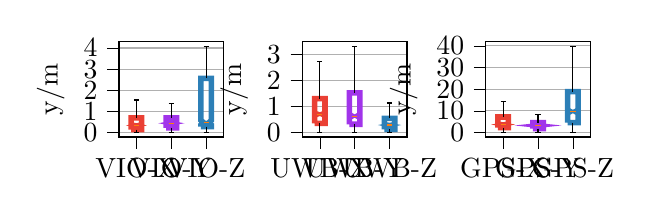
\begin{tikzpicture}

\definecolor{color0}{rgb}{0.91796875,0.25,0.203125}
\definecolor{color1}{rgb}{1,0.498039215686275,0.0549019607843137}
\definecolor{color2}{rgb}{0.6328125,0.203125,0.91796875}
\definecolor{color3}{rgb}{0.171875,0.49609375,0.71875}

\begin{groupplot}[group style={group size=3 by 1}]
\nextgroupplot[
            height=\figureheight,
            width=\figurewidth,
tick align=outside,
tick pos=left,
x grid style={white!69.0196078431373!black},
xmin=2.5, xmax=5.5,
xtick={3,4,5}, 
xticklabels={VIO-X,VIO-Y,VIO-Z},
xtick style={color=black},
y grid style={white!69.0196078431373!black},
ylabel={y/m},
ymajorgrids,
ymin=-0.2041598322165, ymax=4.2888497382065,
ytick style={color=black}
]
\addplot [line width=2pt, color0]
table {%
2.85 0.14334829911975
3.15 0.14334829911975
3.15 0.313649677813772
3.075 0.340273547968
3.15 0.366897418122227
3.15 0.703215187335025
2.85 0.703215187335025
2.85 0.366897418122227
2.925 0.340273547968
2.85 0.313649677813772
2.85 0.14334829911975
};
\addplot [black]
table {%
3 0.14334829911975
3 0.000565849789999906
};
\addplot [black]
table {%
3 0.703215187335025
3 1.5407297163
};
\addplot [black]
table {%
2.925 0.000565849789999906
3.075 0.000565849789999906
};
\addplot [black]
table {%
2.925 1.5407297163
3.075 1.5407297163
};
\addplot [line width=2pt, color2]
table {%
3.85 0.23068461689975
4.15 0.23068461689975
4.15 0.421681808783881
4.075 0.443865155955
4.15 0.466048503126119
4.15 0.6971728276275
3.85 0.6971728276275
3.85 0.466048503126119
3.925 0.443865155955
3.85 0.421681808783881
3.85 0.23068461689975
};
\addplot [black]
table {%
4 0.23068461689975
4 6.78755300000944e-05
};
\addplot [black]
table {%
4 0.6971728276275
4 1.37052999886
};
\addplot [black]
table {%
3.925 6.78755300000944e-05
4.075 6.78755300000944e-05
};
\addplot [black]
table {%
3.925 1.37052999886
4.075 1.37052999886
};
\addplot [line width=2pt, color3]
table {%
4.85 0.2863183199475
5.15 0.2863183199475
5.15 0.366798369904502
5.075 0.47536206777
5.15 0.583925765635498
5.15 2.5692779101575
4.85 2.5692779101575
4.85 0.583925765635498
4.925 0.47536206777
4.85 0.366798369904502
4.85 0.2863183199475
};
\addplot [black]
table {%
5 0.2863183199475
5 0.0066105721099996
};
\addplot [black]
table {%
5 2.5692779101575
5 4.08462203046
};
\addplot [black]
table {%
4.925 0.0066105721099996
5.075 0.0066105721099996
};
\addplot [black]
table {%
4.925 4.08462203046
5.075 4.08462203046
};
\addplot [color1]
table {%
2.925 0.340273547968
3.075 0.340273547968
};
\addplot [color1]
table {%
3.925 0.443865155955
4.075 0.443865155955
};
\addplot [color1]
table {%
4.925 0.47536206777
5.075 0.47536206777
};

\nextgroupplot[
            height=\figureheight,
            width=\figurewidth,
tick align=outside,
tick pos=left,
x grid style={white!69.0196078431373!black},
xmin=2.5, xmax=5.5,
xtick={3,4,5}, 
xticklabels={UWB-X,UWB-Y,UWB-Z},
xtick style={color=black},
y grid style={white!69.0196078431373!black},
ylabel={y/m},
ymajorgrids,
ymin=-0.16549055, ymax=3.48031755,
ytick style={color=black}
]
\addplot [line width=2pt, color0]
table {%
2.85 0.3525635
3.15 0.3525635
3.15 0.663919851384457
3.075 0.7092355
3.15 0.754551148615543
3.15 1.30549525
2.85 1.30549525
2.85 0.754551148615543
2.925 0.7092355
2.85 0.663919851384457
2.85 0.3525635
};
\addplot [black]
table {%
3 0.3525635
3 0.000228000000000117
};
\addplot [black]
table {%
3 1.30549525
3 2.730964
};
\addplot [black]
table {%
2.925 0.000228000000000117
3.075 0.000228000000000117
};
\addplot [black]
table {%
2.925 2.730964
3.075 2.730964
};
\addplot [line width=2pt, color2]
table {%
3.85 0.32147575
4.15 0.32147575
4.15 0.579247862826431
4.075 0.6363865
4.15 0.693525137173569
4.15 1.52303025
3.85 1.52303025
3.85 0.693525137173569
3.925 0.6363865
3.85 0.579247862826431
3.85 0.32147575
};
\addplot [black]
table {%
4 0.32147575
4 0.00053700000000001
};
\addplot [black]
table {%
4 1.52303025
4 3.314599
};
\addplot [black]
table {%
3.925 0.00053700000000001
4.075 0.00053700000000001
};
\addplot [black]
table {%
3.925 3.314599
4.075 3.314599
};
\addplot [line width=2pt, color3]
table {%
4.85 0.12925575
5.15 0.12925575
5.15 0.271720993925497
5.075 0.291425
5.15 0.311129006074503
5.15 0.543606500000001
4.85 0.543606500000001
4.85 0.311129006074503
4.925 0.291425
4.85 0.271720993925497
4.85 0.12925575
};
\addplot [black]
table {%
5 0.12925575
5 0.000409999999999577
};
\addplot [black]
table {%
5 0.543606500000001
5 1.136963
};
\addplot [black]
table {%
4.925 0.000409999999999577
5.075 0.000409999999999577
};
\addplot [black]
table {%
4.925 1.136963
5.075 1.136963
};
\addplot [color1]
table {%
2.925 0.7092355
3.075 0.7092355
};
\addplot [color1]
table {%
3.925 0.6363865
4.075 0.6363865
};
\addplot [color1]
table {%
4.925 0.291425
5.075 0.291425
};

\nextgroupplot[
            height=\figureheight,
            width=\figurewidth,
tick align=outside,
tick pos=left,
x grid style={white!69.0196078431373!black},
xmin=2.5, xmax=5.5,
xtick={3,4,5}, 
xticklabels={GPS-X,GPS-Y,GPS-Z},
xtick style={color=black},
y grid style={white!69.0196078431373!black},
ylabel={y/m},
ymajorgrids,
ymin=-1.98942987402609, ymax=41.8011407864614,
ytick style={color=black}
]
\addplot [line width=2pt, color0]
table {%
2.85 2.29513189908015
3.15 2.29513189908015
3.15 3.50118807088244
3.075 3.73463416107142
3.15 3.96808025126039
3.15 7.20421293512076
2.85 7.20421293512076
2.85 3.96808025126039
2.925 3.73463416107142
2.85 3.50118807088244
2.85 2.29513189908015
};
\addplot [black]
table {%
3 2.29513189908015
3 0.00105061054152111
};
\addplot [black]
table {%
3 7.20421293512076
3 14.4110150642539
};
\addplot [black]
table {%
2.925 0.00105061054152111
3.075 0.00105061054152111
};
\addplot [black]
table {%
2.925 14.4110150642539
3.075 14.4110150642539
};
\addplot [line width=2pt, color2]
table {%
3.85 1.89610601252667
4.15 1.89610601252667
4.15 3.17713051610494
4.075 3.30582850812832
4.15 3.4345265001517
4.15 4.60246477615834
3.85 4.60246477615834
3.85 3.4345265001517
3.925 3.30582850812832
3.85 3.17713051610494
3.85 1.89610601252667
};
\addplot [black]
table {%
4 1.89610601252667
4 0.00318968972726463
};
\addplot [black]
table {%
4 4.60246477615834
4 8.54358799637033
};
\addplot [black]
table {%
3.925 0.00318968972726463
4.075 0.00318968972726463
};
\addplot [black]
table {%
3.925 8.54358799637033
4.075 8.54358799637033
};
\addplot [line width=2pt, color3]
table {%
4.85 4.62876387283643
5.15 4.62876387283643
5.15 9.05131237161907
5.075 9.72946982217759
5.15 10.4076272727361
5.15 18.8895719133201
4.85 18.8895719133201
4.85 10.4076272727361
4.925 9.72946982217759
4.85 9.05131237161907
4.85 4.62876387283643
};
\addplot [black]
table {%
5 4.62876387283643
5 0.0193616773566083
};
\addplot [black]
table {%
5 18.8895719133201
5 39.8106603018938
};
\addplot [black]
table {%
4.925 0.0193616773566083
5.075 0.0193616773566083
};
\addplot [black]
table {%
4.925 39.8106603018938
5.075 39.8106603018938
};
\addplot [color1]
table {%
2.925 3.73463416107142
3.075 3.73463416107142
};
\addplot [color1]
table {%
3.925 3.30582850812832
4.075 3.30582850812832
};
\addplot [color1]
table {%
4.925 9.72946982217759
5.075 9.72946982217759
};
\end{groupplot}

\end{tikzpicture}
}
%     \caption{Error during VIO works}
%     \label{fig:uwb_vio_gps_err}
% \end{figure*}

%%%%%%%%%%%%%%%%%%%%%%%%%%%%%%%%%%%%%%%%%%%%%%
%%                                          %%
%%              CONCLUSION                  %%
%%                                          %%
%%%%%%%%%%%%%%%%%%%%%%%%%%%%%%%%%%%%%%%%%%%%%%

% \newpage
\section{Conclusion}\label{sec:conclusion}
This paper has proposed a novel approach for tracking a UAV based on the fusion of signal images and point clouds from an Ouster LiDAR. Unlike conventional LiDAR and camera fusion, this approach does not need any calibration and preprocessing with external cameras and the LiDAR data is more resistant to harsh environments. We collected three different data sequences in an indoor environment with the OptiTrack mocap system providing ground truth positions. We compared the proposed approach with the approaches based on either only point clouds or signal images and the results showed the effectiveness of our proposed approach. Additionally, we found that our approach can be utilized in a popular mobile computing platform, Jetson Nano according to our evaluation.

Future work includes fusing the Ouster images (depth, signal, and ambient), point clouds, and conventional RGB images in various applications including simultaneous localization
and mapping (SLAM), object detection, and tracking.




%%%%%%%%%%%%%%%%%%%%%%%%%%%%%%%%%%%%%%%%%%%%%%
%%                                          %%
%%            ACKNOWLEDGMENT                %%
%%                                          %%
%%%%%%%%%%%%%%%%%%%%%%%%%%%%%%%%%%%%%%%%%%%%%%

\section*{Acknowledgment}

This research work is supported by the Academy of Finland's AutoSOS project (Grant No. 328755) and RoboMesh project (Grant No. 336061).


%%%%%%%%%%%%%%%%%%%%%%%%%%%%%%%%%%%%%%%%%%%%%%
%%                                          %%
%%              BIBLIOGRAPHY                %%
%%                                          %%
%%%%%%%%%%%%%%%%%%%%%%%%%%%%%%%%%%%%%%%%%%%%%%
% \newpage
% \nocite{*}
\bibliographystyle{unsrt}
\bibliography{bibliography}



\end{document}


